\documentclass[14pt,twoside]{extreport}
\usepackage[utf8]{inputenc}
\usepackage{anyfontsize}
\usepackage{fontspec}
\usepackage{xltxtra}
\usepackage[ukrainian]{babel}
\usepackage{xecyr}
\defaultfontfeatures{Scale=MatchLowercase,Mapping=tex-text}
\setmainfont{XITS}
\setsansfont{Journal}

\usepackage{titlesec}    
\titleformat{\chapter}[display]
{\normalfont\filcenter%
    \huge% change this size to your needs for the first line
    \bfseries}{\chaptertitlename\ \thechapter}{16pt}{%
    \Large % change this size to your needs for the second line
    }

\usepackage{amssymb}
\usepackage{amsmath}
\usepackage{polynom}
\usepackage{graphicx}
\usepackage[tableposition=top,singlelinecheck=false]{caption}
\DeclareCaptionLabelFormat{dstufigure}{Рисунок #2}
\DeclareCaptionLabelFormat{dstutable}{Таблиця #2}
\DeclareCaptionLabelSeparator{dstu}{~--~}
\captionsetup{labelsep=dstu}
\captionsetup*[figure]{labelformat=dstufigure}
\captionsetup*[table]{labelformat=dstutable}
\usepackage{xspace}
\usepackage{multirow}
\usepackage{hhline}
\usepackage[a4paper,inner=1.3cm,text={19cm,27.3cm}]{geometry}
\usepackage{pstricks}
\usepackage{mathtools}
\usepackage{mathrsfs}
\usepackage{color}
\usepackage{indentfirst}
\usepackage{enumitem}
\makeatletter
    \AddEnumerateCounter{\asbuk}{\@asbuk}{ю)}
\makeatother
\setlist{nosep, leftmargin=\parindent}
\renewcommand{\labelenumii}{\asbuk{enumii})}
\usepackage{multicol}
\usepackage[unicode,pdfencoding=auto]{hyperref}
\hypersetup{
	colorlinks=true,
	linktoc=all,
	linkcolor=blue,
}
\usepackage{amsthm}
\newtheoremstyle{mystyle}% name
{3pt}% space above
{3pt}% space below
{}% body font
{}% indent amount
{\normalfont\bfseries}% theorem head font
{.}% punctuation after theorem head
{.5em}% space after theorem head
{}% theorem head spec

\theoremstyle{mystyle}

\newtheorem{dfn}{Означення}
\newtheorem{thm}{Теорема}

\renewenvironment{proof}{{\bfseries Доведення.}}{$\blacksquare$}

\newcounter{NumberInTable}
\newcommand{\LTNUM}{\stepcounter{NumberInTable}{(\theNumberInTable)}}

\newcommand{\Laplace}[1]{\ensuremath{\mathcal{L}{\left[#1\right]}}}
\newcommand{\InvLap}[1]{\ensuremath{\mathcal{L}^{-1}{\left[#1\right]}}}

\makeatletter 
\def\@biblabel#1{#1. } 
\makeatother

\usepackage{bbding}

\newcommand{\problems}{\bigskip\noindent\fbox{\HandPencilLeft}\hspace{6pt}\textsf{Задачі
		для самостійного розв'язування}}

\usepackage{makeidx}

\makeindex

\usepackage[affil-it]{authblk}
\title{\huge Конспект лекцій з курсу інтегральних рівнянь та елементів функціонального аналізу}
\author{Ю. О. Чорноіван}

\newcommand\bigfrown[2][\textstyle]{\ensuremath{%
\array[b]{c}\text{\scalebox{2}{$#1\frown$}}\\[-1.3ex]#1#2\endarray}}

\numberwithin{equation}{chapter}

\addto\captionsukrainian{\def\bibname{Використана література}}
\addto\captionsukrainian{\def\chaptername{Лекція}}

\newcommand{\cab}{\mathbb{C}([a; b])}

\begin{document}
\maketitle
\tableofcontents
\newpage
\sloppy

\chapter{Поняття інтегрального рівняння. Класифікація інтегральних рівнянь}

\begin{dfn}
\textbf{Інтегральним рівнянням} називається рівняння, яке містить невідому функцію під знаком інтеграла.
\end{dfn}
Наприклад,
\begin{equation} \label{inteqfred2kind}
\varphi (t)=\lambda \int _{a}^{b} K(t, s)\varphi (t)\mathrm{d}s+f(t), \quad t\in [a;b],
\end{equation}
або
\begin{equation} \label{inteqvolt2kind}
\varphi (t)=\lambda \int _{a}^{t} K(t, s)\varphi (s)\mathrm{d}s+f(t).
\end{equation}
Тут $K(t, s)$, $f(t)$ -- задані функції, $\lambda$ -- комплексний параметр, $\varphi (t)$ -- шуканий розв'язок. Функції $K(t, s)$ та $f(t)$ називаються ядром і вільним членом інтегрального рівняння\index{інтегральне рівняння!ядро}\index{вільний член}.

Найпростіші лінійні інтегральні рівняння класифікуються таким чином:
\begin{enumerate}
	\item Якщо шукана функція міститься тільки під знаком інтеграла, то рівняння називається інтегральним рівнянням першого роду\index{інтегральне рівняння!першого роду}. Прикладами таких рівнянь є
	\begin{equation} \label{eq1_3}
	\int _{a}^{b} K(t, s)\varphi (s)\mathrm{d}s=f(t),
	\end{equation}
	або
	\begin{equation} \label{eq1_4}
	\int _{a}^{t} K(t, s)\varphi (s)\mathrm{d}s=f(t).
	\end{equation}
	Рівняння \eqref{inteqfred2kind} і \eqref{inteqvolt2kind}, в яких шукана функція міститься також і поза інтегральним доданком, називається рівнянням другого роду\index{інтегральне рівняння!другого роду}.
	
	\item Рівняння із фіксованими межами інтегрування вигляду \eqref{inteqfred2kind} і \eqref{eq1_3} називаються інтегральними рівняннями Фредгольма\footnote{Erik Ivar Fredholm (1866 -- 1927) -- шведський математик, відомий здобутками у теорії інтегральних та операторних рівнянь}\index{інтегральне рівняння!Фредгольма}. Якщо ж маємо рівняння зі змінними межами інтегрування вигляду \eqref{inteqvolt2kind} і \eqref{eq1_4}, то такі інтегральні рівняння називають рівнянням Вольтерри\footnote{Vito Volterra (1860 -- 1940) -- італійський математик і фізик, один із засновників функціонального аналізу}\index{інтегральне рівняння!Вольтерри}.
	
	Формально рівняння Вольтерри можна розглядати як частинний випадок рівняння Фредгольма, поклавши, наприклад, в \eqref{inteqvolt2kind} $K(t, s) \equiv 0$ при $s>t$. Однак фізичні задачі, які приводять до рівнянь Вольтерри і Фредгольма, а також властивості розв'язків цих рівнянь істотно різняться. Тому рівняння Вольтерри виокремлюють у власний клас.
	
	\item Рівняння \eqref{inteqfred2kind} -- \eqref{eq1_4} називаються однорідними, якщо $f(t)\equiv 0$. Якщо це не так, ці рівняння називаються неоднорідними.
	
	\item Якщо ядро інтегрального рівняння залежить лише від різниці змінних, $K(t, s) \equiv K(t - s)$, то рівняння називається різницевим. Відповідні інтеграли у рівнянні називаються інтегралами типу \emph{згортки}\index{інтеграли типу згортки}.
\end{enumerate}

\begin{dfn}
Розв'язком інтегрального рівняння називається функція $\varphi (t)$, яка у результаті підставляння до цього рівняння дає тотожність.
\end{dfn}

\textbf{Зауваження.} Тут і надалі, змінну від якої залежить функція можна вважати координатами деякої точки у просторі, а усі інтеграли у рівняннях вважати інтегралами Лебеґа\footnote{Henri L\'{e}on Lebesgue (1875 -- 1941) -- французький математик, відомий роботами з теорії інтеграла}. Втім, заради простоти теоретичних викладень, ми не акцентуватимемо на цьому увагу, розглядаючи лише одновимірні випадки і пишучи звичайні інтеграли Рімана, без використання поняття міри.

Історично, одними з перших відомих інтегральних рівнянь були інтегральні рівняння, пов'язані із інтегральними перетвореннями. Прикладом є рівняння, які визначають перетворення Фур'є
\begin{align*}
&\Phi(\omega)=\displaystyle\int _{-\infty} ^{\infty}  e^{-i\omega t} \varphi(t)\mathrm{d}t,\quad t\in \mathbb{R},\\
&\varphi(t)=\frac{1}{2\pi} \int _{-\infty} ^{\infty}  e^{i\omega t} \Phi(\omega)\mathrm{d}\omega.
\end{align*}

Якщо розглядати одне з цих рівнянь як інтегральне рівняння щодо невідомої функції, то інше рівняння дає розв'язок цього рівняння у вигляді інтеграла від відомої функції (оригіналу чи перетворення).

Важливе місце у розв'язанні задач механіки займають парні інтегральні рівняння\index{інтегральне рівняння!парне}. У випадку одної незалежної змінної такі рівняння можна представити у вигляді
\begin{equation*}
\begin{array}{l}
\displaystyle a \varphi(t) - \int_{-\infty}^{+\infty} K_1(t-s) \varphi(s) \mathrm{d}s = f(t); \quad t>0,\\
\displaystyle b \varphi(t) - \int_{-\infty}^{+\infty} K_2(t-s) \varphi(s) \mathrm{d}s = f(t); \quad t<0,\\
\end{array}
\end{equation*}
де $a$ і $b$ -- сталі. Такі рівняння, зокрема, є наслідком застосування інтегральних перетворень для розв'язування контактних задач теорії пружності.

Особливий клас інтегральних рівнянь являють собою \emph{сингулярні інтегральні рівняння}\index{інтегральне рівняння!сингулярне}. Одновимірне сингулярне рівняння має вигляд
\begin{equation*}
a(t)\varphi(t) - \frac{b(t)}{\pi i} \int_{\Gamma}\frac{\varphi(\zeta)}{\zeta - t} \mathrm{d}\zeta + \int_{\Gamma} K(t, \zeta) \varphi(\zeta) \mathrm{d}\zeta = f(t).
\end{equation*}
Тут $\Gamma$ -- скінченна або зліченна сукупність простих дуг, замкнених або розімкнених, $\zeta$ і $t$ -- комплексні координати точок на $\Gamma$, $a(t)$, $b(t)$ і $f(t)$ -- задані на $\Gamma$ функції. Другий інтеграл у записаній формі рівняння є сингулярним, його значенням вважають головне значення інтеграла (інтеграл типу Коші).

Сингулярні інтегральні рівняння широко використовуються у механіці руйнування та теорії пружності. Методика розв'язування сингулярних інтегральних рівнянь значно відрізняється від методики розв'язування рівнянь без сингулярності, тому у межах цього курсу ми її не розглядатимемо.

Важливим узагальненням лінійних рівнянь є нелінійні інтегральні рівняння. Вигляд таких рівнянь може бути найрізноманітнішим. Втім, серед них виокремлюють такі:
\begin{equation}
\varphi(t) - \int_{\Omega} K(t, s) F(s, \varphi(s)) \mathrm{d}s = 0
\end{equation}
-- інтегральне рівняння Гамерштайна\footnote{Adolf Hammerstein -- німецький математик}\index{інтегральне рівняння!Гамерштайна}.
\begin{equation}
\varphi(t) - \int_{\Omega} K(t, s, \varphi(s)) \mathrm{d}s = 0
\end{equation}
-- інтегральне рівняння Урисона\footnote{Pavel Urysohn (1898 -- 1924) -- російський математик (народився в Одесі), один із засновників топології, співавтор сучасного означення компактності}\index{інтегральне рівняння!Урисона}. Тут $\Omega$ -- деяка обмежена множина. Звичайно ж, відшукання розв'язку нелінійних рівнянь є складнішою задачею за отримання розв'язку лінійних рівнянь. Втім, обчислювальні методики відшукання таких розв'язків є подібними.

\chapter{Приклади задач, розв'язування яких зводиться до розв'язування інтегральних рівнянь}

Розгляньмо деякі прості задачі, розв'язки яких можна знайти за допомогою інтегральних рівнянь.

\section{Задача Абеля}

Задача Абеля -- це історично перша задача, розв'язування якої було виконано за допомогою інтегральних рівнянь\index{задача Абеля}.

\begin{figure}[ht]\centering
	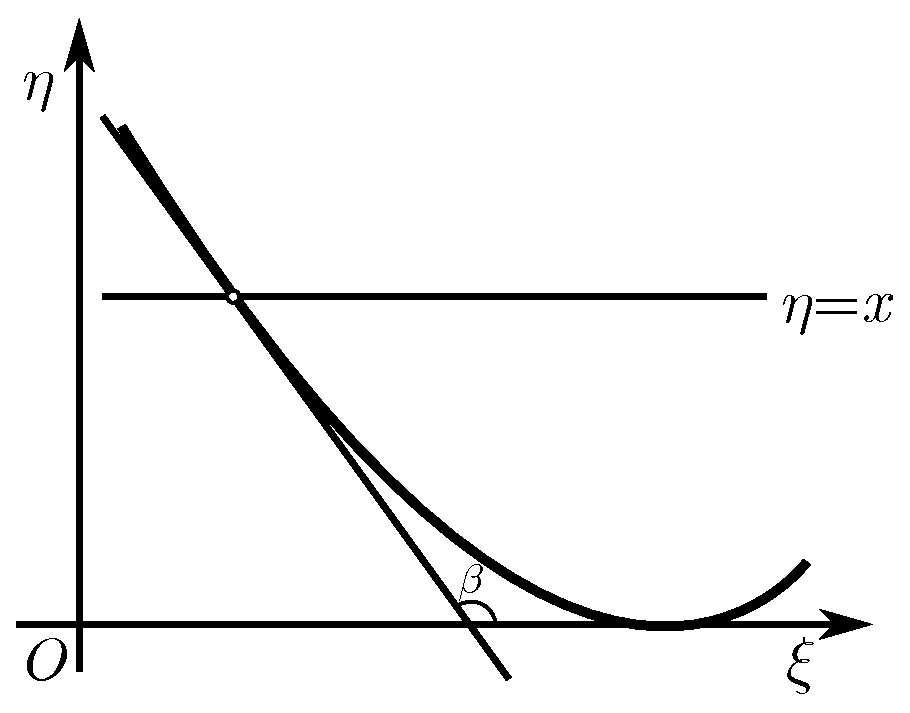
\includegraphics[scale=0.5]{abel.eps}
	\caption{Рух матеріальної точки за таутохроною.}\label{figabel}
\end{figure}

Нехай матеріальна точка, на яку діє сила тяжіння, рухається у вертикальній площині $(\xi ,\eta )$ за деякою кривою (Рис. \ref{figabel}). За умовою задачі слід визначити цю криву так, щоб матеріальна точка, почавши свій рух без початкової швидкості у точці кривої з ординатою $x$, досягла вісі $O\xi$ за час $t=f_{1} (x)$, де $f_{1} (x)$ -- задана функція.

\textbf{Розв'язування.} Абсолютна величина швидкості точки, що рухається під дією сили ваги обчислюється за формулою $v=\sqrt{2g(x-\eta )} $. Нехай $\beta =\beta (\eta )$ -- кут нахилу дотичної до вісі $O\xi $. Тоді матимемо $\dfrac{\mathrm{d}\eta} {\mathrm{d}t} =-\sqrt{2g(x-\eta )} \sin \beta$. Звідси $\mathrm{d}t=-\dfrac{\mathrm{d}\eta} {\sqrt{2g(x-\eta )} \sin \beta}$. Проінтегруємо останній вираз від $0$ до $x$ і покладемо $\dfrac{1}{\sin \beta} =\varphi (\eta )$. Дістанемо
\begin{equation} \label{eq1_5}
    \int _{0}^{x} \frac{\varphi (\eta )}{\sqrt{x-\eta} } \mathrm{d}\eta =-\sqrt{2g} f_{1} (x).
\end{equation}

Нехай $f(x)=-\sqrt{2g} f_{1} (x)$. Тоді \eqref{eq1_5} запишеться у вигляді
\begin{equation} \label{intabeleq}
    \int _{0}^{x} \frac{\varphi (\eta )}{\sqrt{x-\eta} } \mathrm{d}\eta =f(x),
\end{equation}
де $\varphi (\eta )$ -- невідома, а $f(x)$ -- відома функції. Рівняння типу \eqref{intabeleq} називають інтегральним рівнянням Абеля\index{інтегральне рівняння!Абеля}. Воно є частинним випадком лінійного інтегрального рівняння Вольтерри 1-го роду.

З \eqref{intabeleq} визначимо $\varphi (\eta )$ і складемо рівняння шуканої кривої. Дійсно, $\varphi (\eta )=\dfrac{1}{\sin \beta} $, тоді $\eta =\Phi (\beta )$. Далі,
\[\mathrm{d}\xi =\frac{\mathrm{d}\eta} {\tg\beta} =\frac{\Phi '(\beta )\mathrm{d}\beta} {\tg\beta}, \xi =\int  \frac{\Phi '(\beta )}{\tg\beta} \mathrm{d}\beta =\Phi _{1} (\beta).\]
Таким чином, крива визначається параметричними рівняннями: $\xi =\Phi _{1} (\beta )$, $\eta =\Phi (\beta)$. Зокрема, коли $f(x)=C={\rm const}$ такою кривою є циклоїда.

Рівняння Абеля є одним з інтегральних рівнянь, до яких зводиться постановка конкретної задачі механіки чи фізики, без використання проміжних диференціальних рівнянь.

\section{Задача про розподіл яскравості світла}

Згідно із законом геометричної оптики, зображення об'єкта подібне до самого об'єкта. Отже, відрізок відображається у відрізок, при цьому довжина відрізків у загальному випадку різна.

У заданій системі лінз приладу $P$ оберемо масштаб на осях $Ot$ (об'єкта) і $Os$ (спостерігача) так, щоб для двох взаємно відповідних точок $T(t)$ і $S(s)$ мала місце відповідність $t \to s$.

Точка $t$ об'єкта $AB$, що світиться, впливає на освітлення всього зображення $A'B'$, причому найбільша яскравість освітлення у точці $s$. Отже, інтенсивність освітлення $K$ є функцією від $s$ та $t$, тобто $K=K(s,t)$.

Нехай $\eta (t)$ -- щільність яскравості об'єкта. Тоді величина $\eta(t) K(s,t)\Delta t$ визначає наближене значення яскравості зображення у точці $s$, яке породжується елементом об'єкта $\Delta t$, що світиться. У нашому прикладі величина $K(s,t)$ визначається властивостями оптичного приладу $P$.

Яскравість зображення у точці $s$, згідно з принципом суперпозиції, можна наближено подати у вигляді

\begin{equation} \label{eq1_8}
\sum _{k}\eta(t_{k})K(s,t_{k} )\Delta t_{k}
\end{equation}

Нехай довжина відрізка $AB$ дорівнює $l$. Знайдемо границю \eqref{eq1_8} при $\max\limits_{k} \Delta t_{k} \to 0$ і дістанемо розподіл яскравості зображення у вигляді
\begin{equation} \label{eq1_9}
\varphi (s)=\int_{0}^{l} K(s,t) \eta(t)\mathrm{d}t.
\end{equation}

Залежно від постановки фізичної задачі, із \eqref{eq1_9} отримаємо різні типи інтегральних рівнянь. Функція $K(s,t)$ є відомою функцією, що визначається властивостями оптичного приладу. Якщо щільність яскравості зображення $\varphi (s)$ відома, і треба знайти розподіл яскравості об'єкта, який надає задану яскравість зображення, тоді $\varphi (s)$ -- задана функція, $\eta(s)$ -- шукана. Отже, \eqref{eq1_9} -- інтегральне рівняння Фредгольма першого роду. Це рівняння є частинним випадком загальнішого рівняння рендеринґу.

У випадку, коли зображення таке, що крім геометричної подібності, яскравість зображення також подібна яскравості об'єкта, то $\varphi (s)$ і $\eta (s)$ пропорційні, тобто $\varphi (s)=\frac{1}{\lambda} \eta (s)$, і \eqref{eq1_9} перетворюється в однорідне інтегральне рівняння Фредгольма другого роду:
\[
0=\varphi(s)-\lambda \int _{0}^{l} K(s,t)\varphi (t)\mathrm{d}t,
\]
де $\varphi (s)$ -- шукана функція. При цьому виникає питання: чи може коефіцієнт пропорційності мати будь-яке значення, а якщо це не так, то для яких $\lambda$ фізична задача має розв'язок.

Якщо змінити фізичну постановку й вимагати, щоб різниця яскравості між точкою об'єкта й точкою зображення мала всюди задану величину $f(s)=\eta (s)-\varphi (s)$, то підставляючи до \eqref{eq1_9} $\varphi (s)=\eta (s)-f(s)$, отримаємо неоднорідне інтегральне рівняння Фредгольма другого роду:
\[
f(s)=\eta (s)-\lambda \int _{0}^{l} K(s,t)\eta (t)\mathrm{d}t,
\]
де $\eta(s)$ -- шукана функція.

\section{Задача Коші для звичайного лінійного диференційного рівняння n-го порядку з неперервними коефіцієнтами}

Задачу Коші для лінійного диференціального рівняння
\[
\frac{\mathrm{d}^{n} x}{\mathrm{d}t^{n}} + a_{1} (t)\frac{\mathrm{d}^{n-1}x}{\mathrm{d}t^{n-1}} + \ldots +a_{n} (t)x(t)=F(t),
\]
з неперервними коефіцієнтами $a_i(t)$ ($i=\overline{1,n}$) за початкових умов
\begin{equation*}
x(0)=C_{0} , x'(0)=C_{1}, \ldots, x^{(n-1)}(0)=C_{n-1}
\end{equation*}
може бути зведено до інтегрального рівняння Вольтерри 2-го роду.

Продемонструємо методику зведення на прикладі диференційного рівняння 2-го порядку.
\begin{equation} \label{eq1_10}
\frac{\mathrm{d}^{2} x}{\mathrm{d}t^{2}} +a_{1} (t)\frac{\mathrm{d}x}{\mathrm{d}t} +a_{2} (t)x(t)=F(t),
\end{equation}
\begin{equation} \label{eq1_11}
x(0)=C_{0} ,\quad x'(0)=C_{1} .
\end{equation}
Покладемо
\begin{equation} \label{eq1_12}
\frac{\mathrm{d}^{2} x}{\mathrm{d}t^{2}} =\varphi (t).
\end{equation}
Враховуючи початкові умови та формулу
\begin{equation}\label{multintegration}
\underbrace{\int _{0}^{t} \mathrm{d}t\int _{0}^{t} \mathrm{d}t...\int _{0}^{t} } _{n} f(t)\mathrm{d}t=\frac{1}{(n-1)!} \int _{0}^{t} (t-s)^{n-1} f(s)\mathrm{d}s,
\end{equation}
послідовно знаходимо
\begin{equation}\label{eq1_13}
\begin{array}{lll}
\dfrac{\mathrm{d}x}{\mathrm{d}t} &=& \displaystyle\int _{0}^{t} \varphi (s)\mathrm{d}s+C_{1},\\
x(t) &=& \displaystyle \int _{0}^{t} (t-s)\varphi (s)\mathrm{d}s+C_{1} t+C_{0}.
\end{array}
\end{equation}

Беручи до уваги \eqref{eq1_12} та \eqref{eq1_13}, рівняння \eqref{eq1_10} можна записати так:
\begin{equation} \label{eq1_14}
\varphi (t)+\int _{0}^{t} [a_{1} (t)+a_{2} (t)(t-s)]\varphi (s)\mathrm{d}s=F(t)-C_{1} a_{1} (t)-C_{1} ta_{2} (t)-C_{0} a_{2} (t).
\end{equation}
Позначимо
\[K(t, s)=-[a_{1} (t)+a_{2} (t)(t-s)], f(t)=F(t)-C_{1} a_{1} (t)-C_{1} ta_{2} (t)-C_{0} a_{2} (t).\]
Тоді \eqref{eq1_14} набуває вигляду
\begin{equation} \label{eq1_15}
\varphi (t)=\int _{0}^{t} K(t, s)\varphi (s)\mathrm{d}s+f(t).
\end{equation}
Таким чином, задачу Коші \eqref{eq1_10}, \eqref{eq1_11} зведено до розв'язання інтегрального рівняння \eqref{eq1_15}. Знайдену функцію $\varphi (t)$ підставимо у друге співвідношення \eqref{eq1_13} і отримаємо розв'язок $x(t)$ задачі \eqref{eq1_10}, \eqref{eq1_11}.

Існування єдиного розв'язку рівняння \eqref{eq1_15} випливає з існування єдиного розв'язку задачі Коші \eqref{eq1_10}, \eqref{eq1_11} для лінійного диференційного рівняння з неперервними коефіцієнтами в околі точки $t=0$.

Можна показати, що у випадку, коли коефіцієнти $a_{i} (t)$, $i=\overline{1,n}$ сталі, ядро відповідного інтегрального рівняння залежить лише від різниці аргументів $K(t, s)= K(t-s)$, тобто є різницевим.

Отримати відповідні співвідношення для рівняння $n$-го порядку можна аналогічним чином.

\chapter{Теорія Фредгольма розв'язування рівняння Фредгольма 2-го роду}

Повну теорію розв'язування інтегрального рівняння
\begin{equation}\label{feq1}
 \displaystyle \varphi(t)=\lambda\int_{a}^{b}K(t, s)\varphi(s)\mathrm{d}s+f(t)
\end{equation}
з неперервним ядром $K(t, s)$ і вільним членом $f(t)$ при довільних значення параметра $x$ було побудовано Фредгольмом.
Ідея Фредгольма полягає у наступному. Задача розв'язання інтегрального рівняння \eqref{feq1} розглядається як аналітичний аналог алгебраїчної проблеми розв'язання системи $n$ лінійних алгебраїчних рівнянь із $n$ невідомими. А саме, інтеграл у рівнянні \eqref{feq1} замінюється інтегральною сумою, що відповідає розбиттю відрізка $[a; b]$ зміни змінної $s$ на $n$ частин однакової довжини
\[
 \delta=\frac{b-a}{n}.
\]
При цьому, точне рівняння \eqref{feq1} замінюється наближеним
\begin{equation} \label{feqapp}
 \displaystyle \varphi(t)=\lambda\sum_{j=1}^{n}K(t, s_{j})\varphi(s_{j})\delta+f(t),
\end{equation}
де замість $s_{j}$ можна взяти, наприклад, абсциси середин інтервалів розбиття.

Покладаючи у формулі \eqref{feqapp} $t= s_1, s_2, \ldots, s_n$, отримуємо систему лінійних алгебраїчних рівнянь відносно $n$ невідомих $\varphi(s_j)$:
\begin{equation}\label{feqsys}
 \displaystyle \varphi(s_i)=\lambda\sum_{j=1}^{n}K(s_{i}, s_{j})\varphi(s_{j})\delta + f(s_{i})\qquad (i=1, 2, \ldots, n).
\end{equation}

Будемо вважати, що $\varphi(s)$ і $f(s)$ зберігають на $i$-му інтервалі сталі значення, рівні відповідно $\varphi(s_i)$ і $f(s_i)$, а ядро $K(t, s)$ зберігає на кожному частковому квадраті з індексами $i$ і $j$ стале значення, рівне $K(s_i, s_j)$.

Визначник системи \eqref{feqsys}
\begin{equation}
D_n(\lambda)=
\begin{vmatrix}
1-\lambda K(s_1, s_1)\delta & -\lambda K(s_1, s_2)\delta & \ldots & -\lambda K(s_1, s_n)\delta\\
-\lambda K(s_2, s_1)\delta & 1-\lambda K(s_2, s_2)\delta & \ldots & -\lambda K(s_2, s_n)\delta\\
\vdots & \vdots & \ddots & \vdots \\
-\lambda K(s_n, s_1)\delta & -\lambda K(s_n, s_2)\delta & \ldots & 1-\lambda K(s_n, s_n)\delta
\end{vmatrix}
\end{equation}
є поліном відносно $\lambda$.

Якщо $\lambda$ не є коренем полінома $D_n(\lambda)$, то система \eqref{feqsys} має єдиний розв'язок за будь-якої правої частини рівняння, і цей розв'язок може бути знайдено за відомими формулами Крамера. Розв'язуючи систему, ми знайдемо всі $\varphi(s_i)$ і, таким чином, одержимо наближений вираз шуканої функції $\varphi(t)$ у вигляді кусково-сталої функції $\varphi_n(t)$. Метод заміни інтегрального рівняння системою лінійних алгебраїчних рівнянь до сьогодні широко використовується на практиці.

Чим більшим є $n$, тим точніше функція $\varphi_n(t)$ наближає шукану функцію.

У граничному випадку при $n \to \infty$ лінійна система \eqref{feqsys} перетворюється на інтегральне рівняння \eqref{feq1}, а $\varphi_n(t)$ перетворюється на шуканий розв'язок $\varphi(t)$ інтегрального рівняння \eqref{feq1}.

Зрозуміло, що ці міркування мають лише навести на думку щодо характеру розв'язку й потребують обґрунтування.

Можна вчинити трохи інакше. Розв'язавши систему \eqref{feqsys} і підставивши отримані значення $\varphi(s_j)$ до формули \eqref{feqapp}, одержимо наближене аналітичне представлення розв'язку рівняння \eqref{feq1}:
\begin{equation}\label{feqfr}
 \varphi(t)\approx f(t)+\frac{\lambda Q(t,s_{1}.s_{2},\ldots, s_{n};\lambda)}{D_{n}(\lambda)}
\end{equation}
Можна показати, що якщо $K(t,s)$ і $f(t)$ неперервні, чисельник і знаменник другого доданка у \eqref{feqfr} при $\delta = \frac{b-a}{n} \to 0$ прямують відповідно до границь $\lambda\int_{a}^{b}D(t, s;\lambda)f(s)\mathrm{d}s$ та $D(\lambda)$, де $D(\lambda)$ і $D(t, s; \lambda)$ -- деякі цілі функції\footnote{Функція $g(z)$ комплексного аргументу $z$ називається цілою, якщо вона аналітична у всій площині $\mathbb{C}$ комплексної змінної, тобто не має скінченних особливих точок (поліном, $e^z$ тощо).
} від $\lambda$.

Покладаючи
\[
 R(t,s;\lambda) = \frac{D(t,s;\lambda)}{D(\lambda)} \qquad \textrm{резольвента Фредгольма},
\]
одержимо витончену формулу
\begin{equation}\label{resfr}
 \displaystyle \varphi(t)=f(t)+\lambda\int_{a}^{b}R(t, s;\lambda)f(s)\mathrm{d}s,
\end{equation}
за допомогою якої можна отримати розв'язок рівняння \eqref{feq1} для усіх значень $\lambda$, при яких $D(\lambda) \neq 0$.

Фредгольм побудував функції $D(\lambda)$ і $D(t, s; \lambda)$ у вигляді рядів за степенями $\lambda$. Ці ряди було отримано суто формальним граничним переходом, і показано, що при $D(\lambda) \neq 0$ формула \eqref{resfr} визначає єдиний розв'язок рівняння \eqref{feq1}.

Доведення того, що розв'язок системи \eqref{feqsys} при $n \to \infty$ прямує до розв'язку рівняння \eqref{feq1}, було наведено пізніше Гільбертом для випадку неперервного ядра.

Знайдемо вираз для $D(\lambda)$, використовуючи <<правдоподібні міркування>>.

Покладемо $n = 3$. Тоді

\[
D_3(\lambda)=
\begin{vmatrix}
1-\lambda K(s_1, s_1)\delta & -\lambda K(s_1, s_2)\delta & -\lambda K(s_1, s_n)\delta\\
-\lambda K(s_2, s_1)\delta & 1-\lambda K(s_2, s_2)\delta & -\lambda K(s_2, s_n)\delta\\
-\lambda K(s_3, s_1)\delta & -\lambda K(s_3, s_2)\delta & 1-\lambda K(s_3, s_3)\delta
\end{vmatrix}
\]

Покладаючи для скорочення запису $K(s_i, s_j) = K_{ij}$ ($i, j = 1, 2, 3$), будемо мати

\begin{equation}
D_3(\lambda)=(-\lambda\delta)^3
\begin{vmatrix}
K_{11} + t & K_{12} & K_{13}\\
K_{21} & K_{22} + t & K_{23}\\
K_{31} & K_{32} & K_{33} + t
\end{vmatrix}
\end{equation}
де
\[
 t = -1/\lambda\delta.
\]

Покладемо
\begin{equation}\label{fser}
F(t)=
\begin{vmatrix}
K_{11} + t & K_{12} & K_{13}\\
K_{21} & K_{22} + t & K_{23}\\
K_{31} & K_{32} & K_{33} + t
\end{vmatrix}
\end{equation}
Очевидно, що $F(t)$ є поліномом третього степеня відносно $t$. Представимо $F(t)$ за формулою Тейлора за степенями $t$:
\begin{equation}
 F(t)=F(0)+\displaystyle \frac{F'(0)}{1!}t+\frac{F''(0)}{2!}t^{2}+\frac{F'''(0)}{3!}t^{3}.
\end{equation}

З \eqref{fser} випливає, що

\begin{equation}\label{fzero}
F(0)=
\begin{vmatrix}
K_{11} & K_{12} & K_{13}\\
K_{21} & K_{22} & K_{23}\\
K_{31} & K_{32} & K_{33}
\end{vmatrix}
\end{equation}

За правилом диференціювання визначника
\begin{equation}\label{fder}
F'(t)=
\begin{vmatrix}
1 & K_{12} & K_{13}\\
0 & K_{22} + t & K_{23}\\
0 & K_{32} & K_{33} + t
\end{vmatrix}+
\begin{vmatrix}
K_{11} + t & 0 & K_{13}\\
K_{21} & 1 & K_{23}\\
K_{31} & 0 & K_{33} + t
\end{vmatrix}+
\begin{vmatrix}
K_{11} + t & K_{12} & 0\\
K_{21} & K_{22} + t & 0\\
K_{31} & K_{32} & 1
\end{vmatrix},
\end{equation}
отже
\begin{equation}\label{fderzer0}
F'(0)=
\begin{vmatrix}
K_{22} & K_{23}\\
K_{32} & K_{33}
\end{vmatrix}+
\begin{vmatrix}
K_{11} & K_{13}\\
K_{31} & K_{33}
\end{vmatrix}+
\begin{vmatrix}
K_{11} & K_{12}\\
K_{21} & K_{22}\\
\end{vmatrix},
\end{equation}
Таким чином, величина $F'(0)$ дорівнює сумі визначників, які отримуються з визначника \eqref{fzero} викреслюванням $i$-ro стовпця та $i$-го рядка. Неважко бачити, що
\begin{equation}\label{fderzer}
F'(0)=\dfrac{1}{2!}
\sum\limits_{\alpha_1=1}^{3}\sum\limits_{\alpha_2=1}^{3}
\begin{vmatrix}
K_{\alpha_1\alpha_1} & K_{\alpha_1\alpha_2}\\
K_{\alpha_2\alpha_1} & K_{\alpha_2\alpha_2}
\end{vmatrix},
\end{equation}
Насправді, при $\alpha_1 = \alpha_2$ визначники у правій частині \eqref{fderzer} дорівнюють нулю, а визначники, що отримуються один з одного перестановкою індексів $\alpha_1$ і $\alpha_2$, рівні між собою. Звідси випливає справедливість формули \eqref{fderzer}.

Аналогічно, величина $F(0)$ може бути представлена у вигляді

\begin{equation}\label{fzer2}
F(0)=\dfrac{1}{3!}
\sum\limits_{\alpha_1=1}^{3}\sum\limits_{\alpha_2=1}^{3}\sum\limits_{\alpha_3=1}^{3}
\begin{vmatrix}
K_{\alpha_1\alpha_1} & K_{\alpha_1\alpha_2} & K_{\alpha_1\alpha_3}\\
K_{\alpha_2\alpha_1} & K_{\alpha_2\alpha_2} & K_{\alpha_2\alpha_3}\\
K_{\alpha_3\alpha_1} & K_{\alpha_3\alpha_2} & K_{\alpha_3\alpha_3}
\end{vmatrix},
\end{equation}

Диференціюючи \eqref{fder} за $t$ і покладаючи потім $t = 0$, знаходимо
\[
 F''(0) = K_{33} + K _{22} + K_{33} + K_{11} + K_{22} + K_{11},
\]
тобто $F''(0)$ дорівнює сумі <<визначників>> першого порядку, які отримуються з \eqref{fzero} викреслюванням двох рядків із номерами $i$ та $j$ та двох стовпчиків із тими самими номерами:
\begin{equation}\label{eqdder}
 F''(0)=2\sum\limits_{\alpha_1=1}^{3}K_{\alpha_1\alpha_1}.
\end{equation}

І нарешті, $F'''(t)=6$.

Таким чином,

\begin{multline}\label{ft}
F(t)=\dfrac{1}{3!}
\sum\limits_{\alpha_1=1}^{3}\sum\limits_{\alpha_2=1}^{3}\sum\limits_{\alpha_3=1}^{3}
\begin{vmatrix}
K_{\alpha_1\alpha_1} & K_{\alpha_1\alpha_2} & K_{\alpha_1\alpha_3}\\
K_{\alpha_2\alpha_1} & K_{\alpha_2\alpha_2} & K_{\alpha_2\alpha_3}\\
K_{\alpha_3\alpha_1} & K_{\alpha_3\alpha_2} & K_{\alpha_3\alpha_3}
\end{vmatrix}+\\
+\dfrac{1}{2!}
\sum\limits_{\alpha_1=1}^{3}\sum\limits_{\alpha_2=1}^{3}
\begin{vmatrix}
K_{\alpha_1\alpha_1} & K_{\alpha_1\alpha_2}\\
K_{\alpha_2\alpha_1} & K_{\alpha_2\alpha_2}
\end{vmatrix}\dfrac{t}{1!}+
2\sum\limits_{\alpha_1=1}^{3}K_{\alpha_1\alpha_1}\dfrac{t^2}{2!}+6\dfrac{t^3}{3!}.
\end{multline}

Заміняючи у \eqref{ft} $t$ на $-1/\lambda\delta$, отримаємо

\begin{multline*}
D_3(\lambda)=(-\lambda\delta)^3 F(t)= 1 -
\dfrac{\lambda}{1!}\sum\limits_{\alpha_1=1}^{3}K_{\alpha_1\alpha_1}\delta +\\
+\dfrac{\lambda^2}{2!}
\sum\limits_{\alpha_1=1}^{3}\sum\limits_{\alpha_2=1}^{3}
\begin{vmatrix}
K_{\alpha_1\alpha_1} & K_{\alpha_1\alpha_2}\\
K_{\alpha_2\alpha_1} & K_{\alpha_2\alpha_2}
\end{vmatrix}\delta^2-
\dfrac{\lambda^3}{3!}\sum\limits_{\alpha_1=1}^{3}\sum\limits_{\alpha_2=1}^{3}\sum\limits_{\alpha_3=1}^{3}
\begin{vmatrix}
K_{\alpha_1\alpha_1} & K_{\alpha_1\alpha_2} & K_{\alpha_1\alpha_3}\\
K_{\alpha_2\alpha_1} & K_{\alpha_2\alpha_2} & K_{\alpha_2\alpha_3}\\
K_{\alpha_3\alpha_1} & K_{\alpha_3\alpha_2} & K_{\alpha_3\alpha_3}
\end{vmatrix}\delta^3.
\end{multline*}

Аналогічно одержуємо для будь-якого $n$:

\[
\begin{array}{l}
D_n(\lambda)= 1 +
\sum\limits_{m=1}^{n}\dfrac{(-1)^m\lambda^m}{m!}\sum\limits_{\alpha_1=1}^{n}\ldots\sum\limits_{\alpha_m=1}^{n}
\begin{vmatrix}
K_{\alpha_1\alpha_1} & K_{\alpha_1\alpha_2} & \ldots & K_{\alpha_1\alpha_m}\\
K_{\alpha_2\alpha_1} & K_{\alpha_2\alpha_2} & \ldots & K_{\alpha_2\alpha_m}\\
\ldots & \ldots & \ldots & \ldots\\
K_{\alpha_m\alpha_1} & K_{\alpha_m\alpha_2} & \ldots & K_{\alpha_m\alpha_m}
\end{vmatrix}\delta^m.
\end{array}
\]

Зазначимо, що сума
\[
 \sum\limits_{\alpha_1=1}^{n}K_{\alpha_1\alpha_1}\delta = \sum\limits_{j=1}^{n}K(s_j, s_j)\delta
\]
у граничному випадку $\delta \to 0$ переходить в інтеграл $\int_{a}^{b} K(s, s) \mathrm{d}s$, так званий \emph{слід ядра} $K(t,s)$.

Точно так само при $\delta \to 0$ сума
\[
 \sum\limits_{m=1}^{n}\dfrac{(-1)^m\lambda^m}{m!}\sum\limits_{\alpha_1=1}^{n}\ldots\sum\limits_{\alpha_m=1}^{n}
\begin{vmatrix}
K_{\alpha_1\alpha_1} & K_{\alpha_1\alpha_2} & \ldots & K_{\alpha_1\alpha_m}\\
K_{\alpha_2\alpha_1} & K_{\alpha_2\alpha_2} & \ldots & K_{\alpha_2\alpha_m}\\
\ldots & \ldots & \ldots & \ldots\\
K_{\alpha_m\alpha_1} & K_{\alpha_m\alpha_2} & \ldots & K_{\alpha_m\alpha_m}
\end{vmatrix}\delta^m
\]
переходить в інтеграл
\begin{equation}\label{c_m}
C_m = \int_{a}^{b}\ldots \int_{a}^{b}
\begin{vmatrix}
K(\alpha_1, \alpha_1) & K(\alpha_1, \alpha_2) & \ldots & K(\alpha_1, \alpha_m)\\
K(\alpha_2, \alpha_1) & K(\alpha_2, \alpha_2) & \ldots & K(\alpha_2, \alpha_m)\\
\ldots & \ldots & \ldots & \ldots\\
K(\alpha_m, \alpha_1) & K(\alpha_m, \alpha_2) & \ldots & K(\alpha_m, \alpha_m)
\end{vmatrix}\mathrm{d}\alpha_1\ldots\mathrm{d}\alpha_m
\end{equation}

Позначаючи через $D(\lambda)$ границю $D_n(\lambda)$ при $n \to \infty$, матимемо
\begin{equation}\label{dser}
 D(\lambda)=\sum_{m=0}^{\infty}\frac{(-1)^{m}}{m!}C_{m}\lambda^{m}
\end{equation}
де $C_m$ визначаються за формулами \eqref{c_m}, причому $C_0 = 1$.

Покажемо, що ряд \eqref{dser} збігається всюди, тобто $D(\lambda)$ є цілою функцією $\lambda$. Скористаємося нерівністю Адамара\footnote{Jacques Salomon Hadamard (1865 -- 1963) -- французький математик, відомий внеском у теорію чисел, теорію функцій комплексної змінної, диференціальну геометрію та теорію диференціальних рівнянь у частинних похідних}: якщо $\Delta$ -- визначник $n$-го порядку
\[
\Delta=
\begin{vmatrix}
a_{11} & a_{12} & \ldots & a_{1n}\\
a_{21} & a_{22} & \ldots & a_{2n}\\
\ldots & \ldots & \ldots & \ldots\\
a_{n1} & a_{n2} & \ldots & a_{nn}
\end{vmatrix},
\]
то
\begin{equation}\label{hadamard}
 |\Delta|\leqslant \sigma_1\sigma_2\ldots\sigma_n,
\end{equation}
де $\sigma_i^2$ є сумою квадратів елементів $i$-го рядка визначника
\[
 \sigma_i^2 = a_{i1}^2 + a_{i2}^2 + \ldots + a_{in}^2 \quad (i = 1, 2, \ldots, n).
\]
У випадку $n = 3$ ця нерівність має простий геометричний зміст. Справді, вважаючи $a_{i1}$, $a_{i2}$, $a_{i3}$ координатами вектора $\vec{a}_i$ ($i = 1, 2, 3$), знаходимо, що $\Delta$ є мішаним добутком векторів $\vec{a}_1$, $\vec{a}_2$, $\vec{a}_3$, яке за абсолютною величиною дорівнює об'єму паралелепіпеда, побудованого на векторах $\vec{a}_1$, $\vec{a}_2$, $\vec{a}_3$. Величини $\sigma_1$, $\sigma_2$, $\sigma_3$ визначають довжини цих векторів, довжини ребер паралелепіпеда. Нерівність \eqref{hadamard} Адамара виражає у цьому випадку очевидний геометричний факт: об'єм паралелепіпеда не може бути більшим добутку довжин його ребер.

Нерівність перетворюється на рівність тільки у тому випадку, коли паралелепіпед прямокутний, тобто коли вектори $\vec{a}_1$, $\vec{a}_2$, $\vec{a}_3$ попарно ортогональні.

Нехай $|K(t, s)|\leqslant M$ для усіх $t$, $s$, $a\leqslant t, s \leqslant b$. Тоді для $C_m$ маємо наступну оцінку:
\[
 |C_{m}|\leqslant \int_{a}^{b}\ldots\int_{a}^{b} M^{m}m^{m/2}\mathrm{d}\alpha_{1}\ldots \mathrm{d}\alpha_{m}=M^{m}m^{m/2}(b-a)^{m}.
\]
Отже, ряд \eqref{dser} допускає мажоранту
\begin{equation}\label{majorser}
 1+\displaystyle \sum\limits_{m=1}^{\infty}\frac{m^{m/2}}{m!}[M(b-a)]^{m}\lambda^{m}.
\end{equation}
Радіус збіжності ряду \eqref{majorser}
\begin{multline*}
  R=\displaystyle \lim_{m\to\infty}\frac{M^{m}(b-a)^{m}m^{m/2}(m+1)!}{m!M^{m+1}(b-a)^{m+1}(m+1)^{m+1/2}}=\\
  =\displaystyle\frac{1}{M(b-a)}\lim\limits_{m\to\infty}\frac{m+1}{\sqrt{m+1}\left(1+\frac{1}{m}\right)^{m/2}}=\infty.
\end{multline*}

Значить, ряд \eqref{dser} також збігається при всіх значеннях $\lambda$ і визначає цілу функцію $D(\lambda)$, яку називають \emph{визначником Фредгольма}\index{визначник Фредгольма}.

Аналогічно можна встановити, що функція $D(t, s; \lambda)$ визначається рядом Фредгольма
\begin{equation}\label{dtsser}
 D(t, s; \lambda)=\sum^{\infty}_{m=0}(-1)^{m}\frac{\lambda^{m}}{m!}B_{m}(t, s),
\end{equation}
де
\begin{equation}\label{b_m}
B_m(t, s) = \int_{a}^{b}\ldots \int_{a}^{b}
\begin{vmatrix}
K(t, s) & K(t, \alpha_1) & \ldots & K(t, \alpha_m)\\
K(\alpha_1, s) & K(\alpha_1, \alpha_1) & \ldots & K(\alpha_1, \alpha_m)\\
\ldots & \ldots & \ldots & \ldots\\
K(\alpha_m, s) & K(\alpha_m, \alpha_1) & \ldots & K(\alpha_m, \alpha_m)
\end{vmatrix}\mathrm{d}\alpha_1\ldots\mathrm{d}\alpha_m
\end{equation}
причому $B_0 (t, s) = K(t, s)$. Зазначимо, що
\[
 C_n=\int_{a}^{b}B_{n-1}(t, t) \mathrm{d}t, \quad n>0\quad (C_0=1).
\]
Ряд \eqref{dtsser} збігається при всіх значеннях $\lambda$, тому $D(t, s; \lambda)$ є цілою аналітичною функцією $\lambda$. Її називають \emph{мінором визначника Фредгольма}\index{мінор визначника Фредгольма}.

Таким чином, \emph{резольвента Фредгольма}\index{резольвента Фредгольма}
\begin{equation}\label{resdeg}
 R(t,s;\lambda)=\frac{D(t,s;\lambda)}{D(\lambda)}
\end{equation}
не залежить від $f(t)$ і являє собою частку двох цілих аналітичних функцій, тобто є мероморфною функцією від $\lambda$.

У будь-якій скінченній частині $\lambda$-площини вона може мати як особливі точки лише полюси у скінченній кількості.

Полюсами резольвенти можуть бути тільки нулі $D(\lambda)$. Виконується і обернене твердження: нулі $D(\lambda)$ є полюсами резольвенти.

Формули Фредгольма \eqref{dser} і \eqref{dtsser} надають змогу побудувати розв'язувальне ядро $R(t, s; \lambda)$ інтегрального рівняння \eqref{feq1}.

Незручність користування цими формулами полягає у тому, що ряди \eqref{dser}, \eqref{dtsser}, як правило, складні для обчислення через кратні інтеграли, що визначають коефіцієнти рядів.

Значення $\lambda$, для яких існує резольвента рівняння Фредгольма, будемо називати \emph{регулярними}\index{значення!регулярне}, а значення $\lambda$, для яких резольвента не існує, -- \emph{характеристичними}\index{значення!характеристичне}. Характеристичні числа збігаються з полюсами резольвенти або, що те ж саме, з нулями $D(\lambda)$.

Фундаментальний результат Фредгольма ми можемо тепер сформулювати так:

\emph{Якщо значення $\lambda$ регулярне, то інтегральне рівняння \eqref{feq1}, з неперервним ядром $K(t, s)$ і правою частиною $f(t)$ має єдиний неперервний розв'язок, який дається формулою}
\[
\varphi(t)=f(t)+\lambda\int_{a}^{b}R(t, s;\lambda)f(s)\mathrm{d}s.
\]

Як наслідок дістаємо: якщо $\lambda$ регулярне, то однорідне рівняння
\[
\varphi(t)=\lambda\int_{a}^{b}K(t, s)\varphi(s)\mathrm{d}s.
\]
має лише тривіальний розв'язок $\varphi(t) \equiv 0$.

Тому, якщо однорідне рівняння має нетривіальні розв'язки, то це можливе тільки тоді, коли значення $\lambda$ характеристичне. Нетривіальні розв'язки однорідного інтегрального рівняння називаються \emph{власними} або \emph{фундаментальними функціями} ядра $K(t, s)$\index{функції!власні}\index{функції!фундаментальні}, що відповідають даному характеристичному числу.

Оскільки $D(\lambda)$ є цілою функцією від $\lambda$, не рівною тотожно нулеві ($D(0) = 1$), то, як це випливає із загальної теорії функцій, множина нулів $D(\lambda)$ не може мати граничної точки у обмеженій області площини $\lambda$.

Отже, у будь-якому крузі $|\lambda|<R$ таких нулів може бути лише скінченна кількість. Проведемо кола у комплексній $\lambda$-площині із центром у початку координат і радіусами 1, 2, 3,  … Ці кола розіб'ють площину на зліченну множину областей. У колі будь-якого радіуса $n$ міститься скінченна кількість нулів $D(\lambda)$, і, виходить, у кожному кільці $n < |\lambda| < n + 1$ їх теж міститься лише скінченна кількість. Тому множина всіх нулів $D(\lambda)$ є об'єднанням зліченної множини скінченних множин, отже, є не більше ніж зліченною. Нулі функції $D(\lambda)$ є характеристичними числами ядра $K(t, s)$, тому рівняння Фредгольма \eqref{feq1} з неперервним ядром $K(t, s)$ має не більше зліченної множини характеристичних чисел, які можуть згущуватися тільки на нескінченності.

\section{Інтегральні рівняння з виродженим ядром. Теореми Фредгольма. Альтернатива Фредгольма}\label{thmsfred}

Розглянемо один частинний вигляд інтегральних рівнянь Фредгольма 2-го роду, на прикладі яких чітко можна бачити основні результати фредгольмової теорії таких рівнянь.
\begin{dfn} Ядро $K(t, s)$ інтегрального рівняння називається виродженим, якщо його можна представити у вигляді скінченної суми добутків двох функцій, з яких одна залежить тільки від $t$, а інша тільки від $s$:
\begin{equation}\label{degker}
 K(t, s)=\sum_{i=1}^{n}a_{i}(t)b_{i}(s).
\end{equation}
\end{dfn}

Будемо вважати, що функції $a_i(t)$, так само як і функції $b_i(s)$, між собою лінійно незалежні (у протилежному випадку можна було б зменшити кількість доданків у сумі \eqref{degker}).

Припустимо, що функції $a_i(t)$ і $b_i(s)$ неперервні відрізку $[a; b]$ зміни їхніх аргументів; тоді ядро $K(t, s)$ буде неперервним у прямокутнику $Q=\{a\leqslant t, s \leqslant b\}$.

Розглянемо інтегральне рівняння Фредгольма 2-го роду з виродженим ядром $K(t, s)$:
\begin{equation}\label{degeq}
 \displaystyle \varphi(t)=\lambda\sum_{i=1}^{n}a_{i}(t)\int_{a}^{b}b_{i}(s)\varphi(s)\mathrm{d}s+f(t)
\end{equation}
де $f(t)$ -- неперервна на відрізку $[a; b]$ функція.

Нехай рівняння \eqref{degeq} має розв'язок $\varphi = \varphi(t)$. Покладемо
\begin{equation}\label{c_i}
 c_{i}=\displaystyle \int_{a}^{b}\varphi(s)b_{i}(s)\mathrm{d}s (i=1, 2, \ldots, n)
\end{equation}

Тоді з \eqref{degeq} дістанемо
\begin{equation}\label{degsubst}
\varphi(t)=f(t)+\lambda\sum_{i=1}^{n}c_{i}a_{i}(t)
\end{equation}
звідки видно, що розв'язок інтегрального рівняння з виродженим ядром зводиться до визначення сталих $c_i$ ($i = 1, 2, \ldots, n$). Замінимо у рівності \eqref{degsubst} індекс підсумовування $i$ на $j$, помножимо обидві частини цієї рівності на $b_i(t)$ і проінтегруємо за $t$ у межах від $a$ до $b$:
\begin{equation}\label{substint}
  \displaystyle\int_{a}^{b}\varphi(t)b_{i}(t)\mathrm{d}t=\int_{a}^{b}f(t)b_{i}(t)\mathrm{d}t+ \lambda\sum_{j=1}^{n}c_{j}\int_{a}^{b}a_{j}(t)b_{i}(t)\mathrm{d}t \quad (i=1, 2, \ldots, n).
\end{equation}
Вводячи позначення
\[
 \int_{a}^{b}a_{j}(t)b_{i}(t)\mathrm{d}t=k_{ij}, \displaystyle \int_{a}^{b}f(t)b_{i}(t)\mathrm{d}t=f_{i},
\]
дістанемо систему лінійних алгебраїчних рівнянь, якій мають задовольняти коефіцієнти $c_i$:
\begin{equation}\label{sysc_i}
 c_{i} - \lambda\sum_{j=1}^{n}k_{ij}c_{j}=f_{i}\quad (i=1, 2, \ldots, n).
\end{equation}
Якщо ця система нерозв'язна, то, очевидно, інтегральне рівняння \eqref{degeq} також нерозв'язне.

Нехай тепер система \eqref{sysc_i} має розв'язок $c_1$, $c_2$, \ldots, $c_n$. Підставивши ці значення коефіцієнтів до формули \eqref{degsubst}, дістанемо функцію $\varphi(t)$, яка є розв'язком інтегрального рівняння \eqref{degeq}, у чому неважко переконатися безпосередньою перевіркою.

Таким чином, інтегральне рівняння \eqref{degeq} і система лінійних алгебраїчних рівнянь \eqref{sysc_i} еквівалентні у тому сенсі, що з можливості розв'язання системи \eqref{sysc_i} випливає можливість розв'язання рівняння \eqref{degeq} і навпаки.

Визначник системи \eqref{sysc_i} $D(\lambda)$ дорівнює
\begin{equation}
D(\lambda)=
\begin{vmatrix}
1-\lambda k_{11} & -\lambda k_{12} & \ldots & -\lambda k_{1n}\\
-\lambda k_{21} & 1-\lambda k_{22} & \ldots & -\lambda k_{2n}\\
\vdots & \vdots & \ddots & \vdots \\
-\lambda k_{n1} & -\lambda k_{n2} & \ldots & 1-\lambda k_{nn}
\end{vmatrix}
\end{equation}
і є поліномом відносно $\lambda$ степеня не вище $n$, не дорівнює тотожно нулеві, оскільки
\begin{equation}
D(0)=
\begin{vmatrix}
1 & 0 & \ldots & 0\\
0 & 1 & \ldots & 0\\
\vdots & \vdots & \ddots & \vdots \\
0 & 0 & \ldots & 1
\end{vmatrix}=1.
\end{equation}
Отже, $D(\lambda)$ має не більше $n$ різних коренів.

$D(\lambda)$ називають \emph{визначником Фредгольма}\index{визначник Фредгольма} для інтегрального рівняння \eqref{degeq}, а його нулі, тобто корені рівняння $D(\lambda)=0$, називають характеристичними числами ядра $K(t, s)$ або рівняння \eqref{degeq}.

\begin{enumerate}
 \item Якщо $\lambda$ не збігається з жодним з нулів $D(\lambda)$, тобто $D(\lambda)\neq 0$, то система лінійних рівнянь \eqref{sysc_i} однозначно розв'язна за будь-яких правих частин $f_i$ ($i = 1, 2, \ldots, n$).

Отже,
\begin{thm}
Якщо $\lambda$ не є характеристичним числом, то інтегральне рівняння \eqref{degeq} має єдиний розв'язок $\varphi(t)$, що визначається формулою \eqref{degsubst}, при будь-якому вільному члені $f(t)$.
\end{thm}
Це -- перша теорема Фредгольма\index{теорема Фредгольма!перша}.

У випадку $D(\lambda)\neq 0$ відповідне однорідне інтегральне рівняння
\begin{equation}\label{unidegeq}
 \displaystyle \varphi(t)=\lambda\sum_{i=1}^{n}a_{i}(t)\int_{a}^{b}b_{i}(s)\varphi(s)\mathrm{d}s,
\end{equation}
що відповідає випадку $f(t \equiv 0$ на $[a; b]$ має тільки тривіальний розв'язок $\varphi(t) \equiv 0$. Справді, якщо $f(t) \equiv 0$ на $[a; b]$, то всі $f_i$ ($i = 1, 2, \ldots, n$) дорівнюють нулю й система \eqref{sysc_i} буде системою однорідних лінійних рівнянь з визначником, відмінним від нуля. Така система має лише нульовий розв'язок $c_1=c_2= \ldots = c_n = 0$.

Тому першу теорему Фредгольма іноді формулюють так:
\begin{thm}
 Для того щоб рівняння \eqref{degeq} мало єдиний розв'язок за будь-якої функції $f(t)$, необхідно й достатньо, щоб відповідне однорідне рівняння мало тільки тривіальний розв'язок $\varphi(t) \equiv 0$.
\end{thm}

Якщо розв'язувати систему \eqref{sysc_i} за формулами Крамера, а потім визначники, які стоятимуть у чисельниках, розкладати за елементами стовпця вільних членів, дістанемо вирази вигляду
\[
 c_{i}=\frac{1}{D(\lambda)}\sum_{k=1}^{n}D_{ik}(\lambda)f_{k} \quad (i =1, 2 \ldots, n),
\]
де $D_{ik}(\lambda)$ -- деякі поліноми від $\lambda$ степеня не вище $n - 1$.

Підставляючи ці вирази для $c_i$ до формули \eqref{degsubst}, матимемо
\[
 \displaystyle \varphi(t)=f(t)+\lambda\sum_{i=1}^{n}\frac{1}{D(\lambda)}\sum_{k=1}^{n} D_{ik}(\lambda)a_{i}(t)\int_{a}^{b}f(s)b_{k}(s)\mathrm{d}s,
\]
або
\begin{equation}
 \displaystyle \varphi(t)=f(t)+\lambda\int_{a}^{b}R(t, s; \lambda)f(s)\mathrm{d}s,
\end{equation}
де
\begin{equation}
 R(t, s; \lambda)=\frac{1}{D(\lambda)}\sum_{i=1}^{n}\sum_{k=1}^{n}D_{ik}(\lambda) a_{i}(t) b_{k}(s)
\end{equation}

Функція $R(t, s; \lambda)$ є резольвентою (розв'язувальним ядром) інтегрального рівняння \eqref{degeq}. При фіксованих $t$, $s$ вона являє собою дробову раціональну функцію комплексної змінної $\lambda$, і при будь-якому значенні $\lambda$, відмінному від характеристичного, $R(t, s; \lambda)$ є неперервною функцією $t$, $s$.

\item Нехай тепер $\lambda$ збігається з одним з нулів визначника Фредгольма $D(\lambda)$, тобто є характеристичним числом ядра $K(t, s)$.

Тоді визначник системи \eqref{sysc_i} буде дорівнювати нулеві. Відповідна однорідна система
\begin{equation}\label{unic_i}
 c_{i}-\displaystyle \lambda\sum_{i=1}^{n}k_{ij}c_{j}=0
\end{equation}
має при цьому деяку кількість $p$ ($1 \leqslant p < n$) лінійно незалежних ненульових векторів-розв'язків
\[
 \{c_{1}^{(l)}, c_{2}^{(l)}, \ldots, c_{n}^{(l)}\} \quad (l=1, 2, \ldots, p).
\]
Функції
\begin{equation}
 \displaystyle \varphi_{l}(t)=\sum_{i=1}^{n}c_{i}^{(l)}a_{i}(t) \quad (l=1, 2, \ldots, p)
\end{equation}
будуть нетривіальними розв'язками відповідного однорідного інтегрального рівняння
\begin{equation}\label{unideg}
\displaystyle \varphi(t)=\lambda\sum_{i=1}^{n} a_{i}(t)\int_{a}^{b} b_{i}(s)\varphi(s)\mathrm{d}s.
\end{equation}
Як і у загальному випадку рівняння з невиродженим ядром, нетривіальні розв'язки однорідного рівняння називаються \emph{власними} або \emph{фундаментальними функціями} цього рівняння (або ядра $K(t, s)$), що відповідають даному характеристичному числу. Кількість лінійно незалежних функцій, що відповідає даному характеристичному числу, називається його \emph{рангом} або \emph{кратністю}\index{ранг характеристичного числа}\index{кратність характеристичного числа}.

Неважко помітити, що якщо $\varphi_1(t)$ і $\varphi_2(t)$ -- власні функції, що відповідають тому самому характеристичному числу $\lambda$, то їхня сума $\varphi_1(t) + \varphi_2(t)$ буде також власною функцією, що відповідає цьому ж числу $\lambda$. Точно так само, якщо $\varphi(t)$ -- власна функція, то $\alpha\varphi(t)$, де $\alpha$ -- будь-яка стала, буде власною функцією ядра $K(t, s)$.

Таким чином, власні функції $\varphi_i(t)$, що відповідають даному характеристичному числу $\lambda$, утворюють \emph{лінійний простір}, розмірність якого рівна $p$.

Загальним розв'язком однорідного рівняння \eqref{unideg}, що відповідає даному характеристичному числу, буде функція
\begin{equation}
 \displaystyle \varphi(t)=\sum_{l=1}^{p}\alpha_{l}\varphi_{l}(t) ,
\end{equation}
де $\alpha_i$ -- довільні сталі.

Нагадаємо деякі відомості з лінійної алгебри.

Нехай маємо квадратну матрицю порядку $n$
\begin{equation}
 \mathfrak{U}=(\alpha_{ij})_{i=1, 2, \ldots, n}^{j=1, 2, \ldots, n}
\end{equation}
($\alpha_{ij}$ -- дійсні числа).

Матриця $\mathfrak{U}^*$, яку отримують з $\mathfrak{U}$ заміною всіх її рядків відповідними стовпцями і навпаки, називається спряженою до матриці $\mathfrak{U}$. Тому якщо $\mathfrak{U}= (\alpha_{ij})$, то $\mathfrak{U}^* = (\alpha_{ji})$\index{спряжена матриця}.

Якщо дано систему лінійних алгебраїчних рівнянь
\begin{equation}\label{conjsys}
 \mathfrak{U}X=F,
\end{equation}
де
\[
 X=
\begin{pmatrix}
x_1\\
x_2\\
\vdots\\
x_n
\end{pmatrix},\quad
F=
\begin{pmatrix}
F_1\\
F_2\\
\vdots\\
F_n
\end{pmatrix},
\]
то система
\begin{equation}
\mathfrak{U}^*Y=G
\end{equation}
називається \emph{спряженою} із системою \eqref{conjsys}\index{спряжена система}.

Мінором $k$-го порядку матриці $\mathfrak{U}$ називається визначник $k$-ro порядку, складений з елементів $\alpha_{ij}$ матриці $\mathfrak{U}$, розташованих на перетині якихось її $k$ рядків і $k$ стовпців ($k \leqslant n$)\index{мінор матриці}.

Якщо у матриці $\mathfrak{U}$ усі мінори порядку $k>r$ рівні нулеві, а серед її мінорів порядку $r$ є хоч один, відмінний від нуля, то число $r$ називається рангом матриці $\mathfrak{U}$.
\begin{thm}\label{unithm}
 Якщо визначник системи рівний нулеві, то однорідна система $\mathfrak{U}X=0$ і спряжена з нею система $\mathfrak{U}^*Y=0$ мають кожна $p = n - r$ лінійно незалежних розв'язків, де $r$ -- ранг матриці $\mathfrak{U}$.
\end{thm}

Уведемо наступні поняття. Нехай маємо інтегральне рівняння Фредгольма
\begin{equation}\label{feq2}
 \displaystyle \varphi(t)=\lambda\int_{a}^{b}K(t, s)\varphi(s)\mathrm{d}s+f(t)
\end{equation}
\begin{dfn}
    Ядро $K^*(t, s)$, одержане з ядра $K(t, s)$ заміною $t$ на $s$ і навпаки, називається спряженим\footnote{У випадку, коли $K(t, s)$ є комплекснозначною функцією дійсних аргументів $t$, $s$, покладаємо за означенням
\[
K^*(t,s) = \overline{K(s, t)},
\]
де $\overline{K(s, t)}$ означає величину, комплексно спряжену з $K(s,t)$.} з ядром $K(t, s)$\index{спряжене ядро}:
\begin{equation}
 K^*(t,s) = K(s,t).
\end{equation}
\end{dfn}

Рівняння
\begin{equation}
 \psi(t)=\lambda \int_{a}^{b} K^{*}(t, s)\psi(s)\mathrm{d}s+g(t)
\end{equation}
називається спряженим (союзним) з рівнянням \eqref{feq2}\index{рівняння!спряжене}\index{рівняння!союзне}.

Для інтегрального рівняння \eqref{degeq} з виродженим ядром спряжене з ним рівняння має вигляд
\begin{equation}\label{degcon}
 \psi(t)=\lambda \int_{a}^{b} \sum_{i=1}^{n} a_{i}(s)b_{i}(t)\psi(s)\mathrm{d}s+g(t).
\end{equation}
Для нього
\begin{equation}
 \displaystyle \psi(t)=g(t)+\lambda\sum_{i=1}^{n}c_{i}^{*}b_{i}(t),
\end{equation}
де
\begin{equation}
 c_{i}^{*}=\int_{a}^{b} \psi(s) a_i(s) \mathrm{d}s \quad (i=\overline{1, n})
\end{equation}
Якщо $g(t) \equiv 0$, тобто рівняння \eqref{degcon} однорідне, то для визначення $c_{i}^{*}$ дістаємо однорідну систему
\begin{equation}\label{uniconj}
c_{i}^{*}-\displaystyle \lambda\sum_{j=1}^{n}k_{ji}c_{j}^{*}=0,
\end{equation}
спряжену із системою \eqref{unic_i}.

Унаслідок теореми \ref{unithm} обидві ці системи мають однакову кількість $p$ лінійно незалежних векторів-розв'язків.

Якщо $\{c_1^{*(l)}, \ldots, c_n^{*(l)}\}$ ($l=1, 2, \ldots, p$) є ненульовими векторами-розв'язками системи \eqref{uniconj}, то функції
\[
 \psi_{l}(t)=\sum_{i=1}^{n}c_{i}^{*(l)}b_{i}(t) \quad (l=1, 2, \ldots, p)
\]
будуть власними функціями однорідного рівняння
\begin{equation}\label{unidegeq1}
 \displaystyle \psi(t)=\lambda\sum_{i=1}^{n}b_{i}(t)\int_{a}^{b}a_{i}(s)\psi(s)\mathrm{d}s,
\end{equation}
спряженого з рівнянням \eqref{unidegeq}.

Отже,

\begin{thm}
Якщо $\lambda$ є характеристичним число ядра $K(t, s)$, то однорідне інтегральне рівняння \eqref{unideg} і спряжене з ним рівняння \eqref{unidegeq1} мають ту саму скінченну кількість лінійно незалежних власних функцій.\index{теорема Фредгольма!друга}
\end{thm}
Це -- друга теорема Фредгольма.

\item Розглянемо, нарешті, неоднорідне рівняння \eqref{degeq} у випадку, коли $\lambda$ -- характеристичне число.

Як ми зазначали, можливість його розв'язання еквівалентна можливості розв'язання неоднорідної системи \eqref{sysc_i} лінійних алгебраїчних рівнянь.

Скористаємося наступною теоремою.

\begin{thm} Для того щоб неоднорідна система лінійних алгебраїчних рівнянь була розв'язна, необхідно й достатньо, щоб вектор вільних членів цієї системи був ортогональний до усіх векторів-розв'язків спряженої однорідної системи.
\end{thm}

Згідно із цією теоремою, неоднорідна система \eqref{sysc_i} буде розв'язна тоді й тільки тоді, коли вектор $\{f_1, f_2, \ldots, f_n\}$ буде ортогональним до кожного з векторів $\{c_1^{*(l)}, \ldots, c_n^{*(l)}\}$ ($l=1, 2, \ldots, p$), тобто коли
\begin{equation}\label{fort}
 \sum_{i=1}^{n}f_{i}c_{i}^{*(l)}=0 \quad (l=1, 2, \ldots, p).
\end{equation}
Але $f_{i}=\int_{a}^{b}f(t)b_{i}(t)\mathrm{d}t$, і, отже, умову \eqref{fort} можна записати так:
\begin{equation}\label{threecond}
 \int_{a}^{b}f(t)\sum_{i=1}^{n}c_{i}^{*(l)}b_{i}(t)\mathrm{d}t=\int_{a}^{b} f(t)\psi_{l}(t)\mathrm{d}t=0 \quad (l=1, 2, \ldots, p)
\end{equation}

Таким чином,
\begin{thm}
 Неоднорідне інтегральне рівняння \eqref{degeq} з виродженим ядром при характеристичному значенні $\lambda$ буде розв'язним тоді й тільки тоді, коли вільний член $f(t)$ буде ортогональним до усіх розв'язків спряженого однорідного інтегрального рівняння \eqref{unidegeq1}.\index{теорема Фредгольма!третя}
\end{thm}
Це -- третя теорема Фредгольма.

Підкреслимо, що надання відповіді на питання про можливість розв'язання рівняння \eqref{degeq} вимагає перевірки скінченної кількості $p$ умов
\[
 \int_{a}^{b}f(t)\psi_{l}(t)\mathrm{d}t=0 \quad (l=1, 2, \ldots, p).
\]
Якщо ці умови виконано, то рівняння \eqref{degeq} має нескінченну множину розв'язків. Усі ці розв'язки можна описати формулою
\[
 \varphi(t) = \varphi_{\textrm{з. о.}}(t) + \varphi_{\textrm{н.}}(t),
\]
де $\varphi_{\textrm{н.}}(t)$ -- якийсь розв'язок неоднорідного рівняння \eqref{degeq}, а $\varphi_{\textrm{з. о.}}(t)$. -- загальний розв'язок відповідного однорідного рівняння.

Умови \eqref{threecond} будуть очевидно виконані, якщо виконуються умови
\[
 \int_{a}^{b}f(t)b_{i}(t)\mathrm{d}t=0 \quad (i= 1, 2, \ldots, n).
\]

Як наслідок з доведених теорем випливає важлива теорема про альтернативу.

\begin{thm}[Альтернатива Фредгольма]
Якщо однорідне інтегральне рівняння Фредгольма з виродженим ядром має тільки тривіальний розв'язок, то відповідне неоднорідне рівняння завжди має один і лише один розв'язок. Якщо ж однорідне рівняння має нетривіальний розв'язок, то неоднорідне інтегральне рівняння залежно від вільного члена $f(t)$ або зовсім не має розв'язку, або має нескінченну кількість розв'язків.
\end{thm}
\end{enumerate}

Нехай тепер маємо інтегральне рівняння
\begin{equation}\label{geneq}
 \varphi(t)=\lambda \int_{a}^{b} K(t, s)\varphi(s)\mathrm{d}s + f(t)
\end{equation}
з довільним (невиродженим) неперервним ядром $K(t, s)$ і неперервною $f(t)$. Як ми згодом покажемо, якщо побудувати досить близьке до ядра $K(t, s)$ вироджене ядро $H(t, s)$, то, розв'язавши рівняння з виродженим ядром $H(t, s)$, ми дістанемо розв'язок, близький до розв'язку рівняння з ядром $K(t, s)$ при тій же правій частині. Більше того, якщо ми побудуємо послідовність $\{H_n(t, s)\}$ вироджених ядер, рівномірно збіжну до ядра $K(t, s)$, то послідовність розв'язків рівнянь з ядрами $H_n(t, s)$ буде рівномірно збігатися до розв'язку $\varphi(t)$ рівняння \eqref{geneq} з ядром $K(t, s)$.

Способи побудови вироджених ядер, близьких до даного ядра $K(t, s)$, можуть бути абсолютно довільними. Наприклад, ядро $K(t, s)$ можна наближати частковими сумами степеневого або подвійного тригонометричного ряду, якщо ядро $K(t, s)$ розкладається у рівномірно збіжний у прямокутнику $Q=\{a \leqslant t, s \leqslant b\}$ степеневий або тригонометричний ряд, або наближати його алгебраїчними або тригонометричними інтерполяційними поліномами.

\begin{small}
\textbf{Приклад.} Знайти розв'язок інтегрального рівняння
\[
 \varphi(t) = 3t + \int_{0}^{1} t^3 s \varphi(s) \mathrm{d}s.
\]

\textbf{Розв'язування.}

Винесемо з підінтегрального виразу у правій частині рівняння множник $t^3$, який не залежить від змінної інтегрування:
\[
 \int_{0}^{1} t^3 s \varphi(s) \mathrm{d}s= t^3 \int_{0}^{1} s \varphi(s) \mathrm{d}s.
\]
Очевидно, визначений інтеграл за сталим проміжком інтегрування матиме стале значення, яке позначимо $C$:
\begin{equation}\label{ex1ceq}
 C = \int_{0}^{1} s \varphi(s) \mathrm{d}s.
\end{equation}
Тоді, з початкового рівняння
\begin{equation}\label{ex1phieq}
 \varphi(t) = 3t + t^3 C.
\end{equation}
Підставляючи \eqref{ex1phieq} до \eqref{ex1ceq}, дістанемо
\begin{equation}
 C = \int_{0}^{1} s \varphi(s) \mathrm{d}s = \int_{0}^{1} s \left(3s + s^3 C\right) \mathrm{d}s = \left.\left[s^3+C\dfrac{s^5}{5}\right]\right|_{0}^{1} = 1+ \dfrac{C}{5}.
\end{equation}
Звідки
\[
 C=\dfrac{5}{4}.
\]
Отже,
\[
 \varphi(t) = 3t + \dfrac{5}{4} t^3.
\]

\textbf{Приклад.} Знайти розв'язок інтегрального рівняння
\[
 \varphi(t) = 3t^2 + 4 + \int_{0}^{1} \left(t^3 s + t s^3\right)\varphi(s) \mathrm{d}s.
\]

\textbf{Розв'язування.}

Розкриємо дужки у підінтегральному виразі у правій частині рівняння і винесемо з-під інтегралів множники, які не залежать від змінної інтегрування:
\[
 \varphi(t) = 3t^2 + 4 + t^3 \int_{0}^{1} s \varphi(s) \mathrm{d}s + t \int_{0}^{1} s^3 \varphi(s) \mathrm{d}s.
\]
Очевидно, визначені інтеграли за сталим проміжком інтегрування матимуть сталі значення, які позначимо $C_1$ і $C_2$ відповідно:
\begin{align}\label{ex2ceq}
  &C_1 = \displaystyle\int_{0}^{1} s \varphi(s) \mathrm{d}s;\\
  &C_2 = \displaystyle\int_{0}^{1} s^3 \varphi(s) \mathrm{d}s.
\end{align}
Тоді, з початкового рівняння
\begin{equation}\label{ex2phieq}
 \varphi(t) = 3t^2 + 4 + t^3 C_1 + t C_2.
\end{equation}
Підставляючи \eqref{ex2phieq} до \eqref{ex2ceq}, дістанемо
\begin{align*}
  C_1 = \displaystyle\int_{0}^{1} s \varphi(s) \mathrm{d}s = \int_{0}^{1} s \left(3s^2 + 4 + s^3 C_1 + s C_2\right) \mathrm{d}s = \left.\left[\dfrac{3s^4}{4} + 2 s^2 + C_1 \dfrac{s^5}{5} + C_2\dfrac{s^3}{3}\right]\right|_{0}^{1} = \dfrac{11}{4} + \dfrac{C_1}{5} + \dfrac{C_2}{3};\\
  C_2 = \displaystyle\int_{0}^{1} s^3 \varphi(s) \mathrm{d}s = \int_{0}^{1} s^3 \left(3s^2 + 4 + s^3 C_1 + s C_2\right) \mathrm{d}s = \left.\left[\dfrac{s^6}{2} + s^4 + C_1 \dfrac{s^7}{7} + C_2\dfrac{s^5}{5}\right]\right|_{0}^{1} = \dfrac{3}{2} + \dfrac{C_1}{7} + \dfrac{C_2}{5}.
\end{align*}
Звідки
\[
 \left\{
 \renewcommand{\arraystretch}{2.}
 \begin{array}{lll}
 \dfrac{4}{5}C_1 -\dfrac{1}{3}C_2 &=& \dfrac{11}{4};\\
 -\dfrac{1}{7}C_1 +\dfrac{4}{5}C_2 &=& \dfrac{3}{2}.\\
 \end{array}
 \right.
\]
Розв'язуючи цю систему (наприклад, методом Крамера), дістанемо
\[
C_1=\dfrac{2835}{622}; C_2= \dfrac{3345}{1244}.
\]
Отже,
\[
 \varphi(t) = 3t^2 + 4 + \dfrac{2835}{622} t^3 + \dfrac{3345}{1244}t.
\]

\textbf{Приклад.} Знайти розв'язок інтегрального рівняння
\[
\varphi(t) = 3 + \int_{0}^{\pi/2} \cos (t-s) \varphi(s) \mathrm{d}s.
\]

\textbf{Розв'язування.}

Скористаємося для доведення виродженості ядра цього рівняння формулою косинуса різниці. Далі, розкриємо дужки у підінтегральному виразі у правій частині рівняння і винесемо з-під інтегралів множники, які не залежить від змінної інтегрування:
\begin{multline*}
\varphi(t) = 3 + \int_{0}^{\pi/2} \cos(t-s) \varphi(s) \mathrm{d}s = 3 + \int_{0}^{\pi/2} \left(\cos t \cos s + \sin t \sin s \right) \varphi(s) \mathrm{d}s=\\
3 + \cos t \int_{0}^{\pi/2} \cos s \varphi(s) \mathrm{d}s + \sin t \int_{0}^{\pi/2} \sin s \varphi(s) \mathrm{d}s.
\end{multline*}
Очевидно, визначені інтеграли за сталим проміжком інтегрування матимуть сталі значення, які позначимо $C_1$ і $C_2$ відповідно:
\begin{equation}\label{ex3ceq}
\begin{array}{lll}
C_1 &=& \displaystyle\int_{0}^{\pi/2} \cos s \varphi(s) \mathrm{d}s;\\
C_2 &=& \displaystyle\int_{0}^{\pi/2} \sin s \varphi(s) \mathrm{d}s.
\end{array}
\end{equation}
Тоді, з початкового рівняння
\begin{equation}\label{ex3phieq}
\varphi(t) = 3 + C_1 \cos t + C_2 \sin t.
\end{equation}
Підставляючи \eqref{ex3phieq} до \eqref{ex3ceq}, дістанемо
\begin{align*}
C_1 = &\displaystyle\int_{0}^{\pi/2} \cos s \varphi(s) \mathrm{d}s = \int_{0}^{\pi/2} \cos s \left(3 + C_1 \cos s + C_2 \sin s\right) \mathrm{d}s =\\
 = & \left.\left(3 \sin s + \left[\dfrac{s}{2} + \dfrac{\sin 2s}{4}\right] C_1 - \dfrac{C_2}{4}\cos 2s\right)\right|_{0}^{\pi/2} = 3 + \dfrac{\pi}{4} C_1 + \dfrac{C_2}{2};\\
C_2 = &\displaystyle\int_{0}^{\pi/2} \sin s \varphi(s) \mathrm{d}s = \int_{0}^{\pi/2} \sin s \left(3 + C_1 \cos s + C_2 \sin s\right) \mathrm{d}s =\\
= & \left.\left(-3 \cos s + \dfrac{C_1}{4} \cos 2s + \left[\dfrac{s}{2} - \dfrac{\sin 2s}{4}\right] C_2\right)\right|_{0}^{\pi/2} = 3 + \dfrac{C_1}{2} + \dfrac{\pi}{4} C_2.
\end{align*}
Звідки
\[
\left\{
\begin{array}{lll}
\left(1-\dfrac{\pi}{4}\right)C_1 -\dfrac{1}{2}C_2 &=& 3;\\
-\dfrac{1}{2}C_1 +\left(1 - \dfrac{\pi}{4}\right)C_2 &=& 3.\\
\end{array}
\right.
\]
Розв'язуючи цю систему (наприклад, методом Крамера), дістанемо
\[
C_1=C_2=-\dfrac{12}{\pi - 2}.
\]
Отже,
\[
\varphi(t) = 3 - \dfrac{12}{\pi - 2} \cos t - \dfrac{12}{\pi - 2} \sin t.
\]

\problems
\begin{enumerate}
	\item Знайти розв'язок інтегрального рівняння
	\[
	\varphi(t) = 2 t^3 - \int_{0}^{1} 4t^2 \varphi(s) \mathrm{d}s.
	\]
	\item Знайти розв'язок інтегрального рівняння
	\[
	\varphi(t) = 2 t^3 - 3t + \int_{0}^{1} \left(4t^2 s - 2 s^2 t\right) \varphi(s) \mathrm{d}s.
	\]
	\item Знайти розв'язок інтегрального рівняння
	\[
	\varphi(t) = 2 - \int_{0}^{\pi} \sin (t-s) \varphi(s) \mathrm{d}s.
	\]
\end{enumerate} 

\textbf{Приклад.} Знайти характеристичне число та відповідну йому власну функцію ядра рівняння
\[
\varphi(t) = \lambda \int_{0}^{1} e^{3t} \varphi(s) \mathrm{d}s.
\]

\textbf{Розв'язування.}
Виносячи з-під інтеграла у правій частині рівняння $e^{3t}$ і позначаючи
\[
C=\int_{0}^{1} \varphi(s) \mathrm{d}s,
\]
дістанемо
\[
\varphi(t) = \lambda e^{3t} \cdot C,
\]
отже
\[
C=\int_{0}^{1} \varphi(s) \mathrm{d}s = \int_{0}^{1} \lambda e^{3s} \cdot C \mathrm{d}s = \lambda C \left. \dfrac{e^{3s}}{3}\right|_{0}^{1} = C \lambda \dfrac{e^{3}-1}{3}.
\]

Це рівняння матиме нетривіальний розв'язок для $C$, тобто $\lambda$ у ньому буде характеристичним значенням, лише якщо
\[
\lambda = \dfrac{3}{e^{3}-1}.
\]
При цьому, очевидно, власною функцією буде функція $\varphi(t) = C^* e^{3t}$, де $C^*$ -- довільна стала.

\textbf{Приклад.} Знайти характеристичні числа та відповідні їм власні функції ядра рівняння
\[
\varphi(t) = \lambda \int_{0}^{1} \left(3t^3s - s^2 t^2\right) \varphi(s) \mathrm{d}s.
\]

\textbf{Розв'язування.}

Розкриємо дужки у підінтегральному виразі й винесемо з-під кожного з отриманих інтегралів множник, який не залежить від змінної інтегрування:
\[
\varphi(t) = \lambda \left(3t^3\int_{0}^{1} s \varphi(s) \mathrm{d}s - t^2 \int_{0}^{1} s^2 \varphi(s) \mathrm{d}s\right).
\]
Оскільки визначені інтеграли у останньому виразі є сталими значеннями, уведемо позначення
\begin{equation}\label{ex4ceq}
C_1 = \int_{0}^{1} s \varphi(s) \mathrm{d}s; C_2 = \int_{0}^{1} s^2 \varphi(s) \mathrm{d}s.
\end{equation}
Тоді,
\begin{equation}\label{ex4phieq}
\varphi(t) = \lambda \left(3t^3 C_1 - t^2 C_2\right).
\end{equation}
Далі, підставляючи \eqref{ex4phieq} до \eqref{ex4ceq}, матимемо
\begin{align*}
&C_1 = \int_{0}^{1} s \varphi(s) \mathrm{d}s = \lambda \int_{0}^{1} s \left(3s^3 C_1 - s^2 C_2\right) \mathrm{d}s = \lambda\left[\dfrac{3}{5}C_1 - \dfrac{1}{4}C_2\right];\\
&C_2 = \int_{0}^{1} s^2 \varphi(s) \mathrm{d}s = = \lambda \int_{0}^{1} s^2 \left(3s^3 C_1 - s^2 C_2\right) \mathrm{d}s = \lambda\left[\dfrac{1}{2}C_1 - \dfrac{1}{5}C_2\right];
\end{align*}
або
\begin{equation}\label{ex4system}
\left\{
\begin{array}{ccccc}
\left(1-\dfrac{3}{5}\lambda\right) C_1 &+& \dfrac{\lambda}{4} C_2 &=& 0;\\
-\dfrac{\lambda}{2} C_1 &+& \left(1+\dfrac{\lambda}{5}\right) C_2 &=& 0.
\end{array}
\right.
\end{equation}
Ця система лінійних алгебраїчних рівнянь щодо $C_1$ та $C_2$ має нетривіальний розв'язок, лише якщо її визначник дорівнює нулеві, тобто
\[
\Delta = 
\begin{vmatrix}
1-\dfrac{3}{5}\lambda & \dfrac{\lambda}{4}\\
-\dfrac{\lambda}{2} & 1+\dfrac{\lambda}{5}
\end{vmatrix}
=0,
\]
звідки для характеристичних чисел маємо рівняння
\[
\lambda^2 - 80 \lambda + 200=0.
\]
Це рівняння має два розв'язки:
\[
\lambda_1= 40 - 10\sqrt{14}; \lambda_2 = 40+10\sqrt{14},
\]
для кожного з яких рівняння системи \eqref{ex4system} будуть лінійно залежними. Через це, для визначення залежності між $C_1$ і $C_2$ у власній функції вигляду \eqref{ex4phieq} достатньо скористатися одним з них, наприклад першим:
\[
C_2 = \dfrac{4}{\lambda} \left(\dfrac{3}{5}\lambda -1\right)C_1.
\]
Отже, для $\lambda = \lambda_1$ матимемо
\[
C_2 = \dfrac{12\sqrt{14} - 46}{5\sqrt{14} - 20}C_1,
\]
звідки
\[
\varphi(t) = C \left(3t^3 - \dfrac{12\sqrt{14} - 46}{5\sqrt{14} - 20} t^2\right),
\]
де $C$ -- довільна стала.

Аналогічно, для $\lambda = \lambda_2$
\[
C_2 = \dfrac{12\sqrt{14} + 46}{5\sqrt{14} + 20}C_1,
\]
звідки
\[
\varphi(t) = C \left(3t^3 - \dfrac{12\sqrt{14} + 46}{5\sqrt{14} + 20} t^2\right),
\]
де $C$ -- довільна стала.

\textbf{Приклад.} Знайти характеристичні числа та відповідні їм власні функції ядра рівняння
\[
\varphi(t) = \lambda \int_{0}^{\pi/2} \left(\cos 3t \sin s - \sin 2t \sin 2s\right) \varphi(s) \mathrm{d}s.
\]

\textbf{Розв'язування.}

Розкриємо дужки у підінтегральному виразі й винесемо з-під кожного з отриманих інтегралів множник, який не залежить від змінної інтегрування:
\[
\varphi(t) = \lambda \left(\cos 3t\int_{0}^{\pi/2} \sin s \varphi(s) \mathrm{d}s - \sin 2t \int_{0}^{\pi/2} \sin 2s \varphi(s) \mathrm{d}s\right).
\]
Оскільки визначені інтеграли у останньому виразі є сталими значеннями, уведемо позначення
\begin{equation}\label{ex5ceq}
C_1 = \int_{0}^{\pi/2} \sin s \varphi(s) \mathrm{d}s; C_2 = \int_{0}^{\pi/2} \sin 2s \varphi(s) \mathrm{d}s.
\end{equation}
Тоді,
\begin{equation}\label{ex5phieq}
\varphi(t) = \lambda \left(\cos 3t C_1 - \sin 2t C_2\right).
\end{equation}
Далі, підставляючи \eqref{ex5phieq} до \eqref{ex5ceq}, матимемо
\begin{align*}
&C_1 = \int_{0}^{\pi/2} \sin s \varphi(s) \mathrm{d}s = \lambda \int_{0}^{\pi/2} \sin s \left(\cos 3s C_1 - \sin 2s C_2\right) \mathrm{d}s = \lambda\left[-\dfrac{C_1}{2} - \dfrac{2}{3}C_2\right];\\
&C_2 = \int_{0}^{\pi/2} \sin 2s \varphi(s) \mathrm{d}s = \lambda \int_{0}^{\pi/2} \sin 2s \left(\cos 3s C_1 - \sin 2s C_2\right) \mathrm{d}s = \lambda\left[-\dfrac{2}{5}C_1 - \dfrac{\pi}{4}C_2\right];
\end{align*}
або
\begin{equation}\label{ex5system}
\left\{
\begin{array}{ccccc}
\left(1+\dfrac{\lambda}{2}\right) C_1 &+& \dfrac{2}{3} \lambda C_2 &=& 0;\\
\dfrac{2}{5} \lambda C_1 &+& \left(1+\dfrac{\pi}{4}\lambda\right) C_2 &=& 0.
\end{array}
\right.
\end{equation}
Ця система лінійних алгебраїчних рівнянь щодо $C_1$ та $C_2$ має нетривіальний розв'язок, лише якщо її визначник дорівнює нулеві, тобто
\[
\Delta = 
\begin{vmatrix}
1+\dfrac{\lambda}{2} & \dfrac{2}{3} \lambda\\
\dfrac{2}{5} \lambda & 1+\dfrac{\pi}{4}\lambda
\end{vmatrix}
=0,
\]
звідки для характеристичних чисел маємо рівняння
\[
(15\pi-32)\lambda^2 + (30\pi+60) \lambda + 120=0.
\]
Це рівняння має два розв'язки:
\[
\lambda_1= -\frac{\sqrt{15}\,\sqrt{15\,{\pi }^{2}-60\,\pi +316}+15\,\pi +30}{15\,\pi -32}; \lambda_2 = \frac{\sqrt{15}\,\sqrt{15\,{\pi }^{2}-60\,\pi +316}-15\,\pi -30}{15\,\pi -32},
\]
для кожного з яких рівняння системи \eqref{ex5system} будуть лінійно залежними. Через це, для визначення залежності між $C_1$ і $C_2$ у власній функції вигляду \eqref{ex5phieq} достатньо скористатися одним з них, наприклад першим:
\[
C_2 = -\dfrac{3}{2\lambda} \left(1+\dfrac{\lambda}{2}\lambda\right)C_1= \left(-\dfrac{3}{2\lambda}-\dfrac{3}{4}\right)C_1.
\]
Отже, для $\lambda = \lambda_1$ матимемо
\[
C_2 = -\frac{3\,\sqrt{15}\,\sqrt{15\,{\pi }^{2}-60\,\pi +316}-45\,\pi +282}{4\,\sqrt{15}\,\sqrt{15\,{\pi }^{2}-60\,\pi +316}+60\,\pi +120}C_1,
\]
звідки
\[
\varphi(t) = C \left(\cos 3t + -\frac{3\,\sqrt{15}\,\sqrt{15\,{\pi }^{2}-60\,\pi +316}-45\,\pi +282}{4\,\sqrt{15}\,\sqrt{15\,{\pi }^{2}-60\,\pi +316}+60\,\pi +120} \sin 2t\right),
\]
де $C$ -- довільна стала.

Аналогічно, для $\lambda = \lambda_2$
\[
C_2 = -\frac{3\,\sqrt{15}\,\sqrt{15\,{\pi }^{2}-60\,\pi +316}+45\,\pi -282}{4\,\sqrt{15}\,\sqrt{15\,{\pi }^{2}-60\,\pi +316}-60\,\pi -120}C_1,
\]
звідки
\[
\varphi(t) = C \left(\cos 3t + \frac{3\,\sqrt{15}\,\sqrt{15\,{\pi }^{2}-60\,\pi +316}+45\,\pi -282}{4\,\sqrt{15}\,\sqrt{15\,{\pi }^{2}-60\,\pi +316}-60\,\pi -120} \sin 2t\right),
\]
де $C$ -- довільна стала.

\problems
\begin{enumerate}
	\item Знайти характеристичне число та відповідну йому власну функцію ядра рівняння
	\[
	\varphi(t) = \lambda \int_{0}^{1} \sh t \varphi(s) \mathrm{d}s.
	\]
	\item Знайти характеристичні числа та відповідні їм власні функції ядра рівняння
	\[
	\varphi(t) = \lambda \int_{0}^{\pi/2} \left(\cos 3t \sin 4s + \sin 2t \sin 2s\right) \varphi(s) \mathrm{d}s.
	\]
	\item Знайти характеристичні числа та відповідні їм власні функції ядра рівняння
	\[
	\varphi(t) = \lambda \int_{0}^{2} \left(e^{2t-3s} + e^{t-2s}\right) \varphi(s) \mathrm{d}s.
	\]
\end{enumerate} 

\end{small}


\chapter{Принцип стислих відображень та його застосування до інтегральних рівнянь}

\section{Метричні простори}

\begin{dfn}
Множина $M$ називається метричним простором, якщо кожній парі його елементів $x$, $y$ поставлено у відповідність невід'ємне дійсне число $\rho_M(x, y)$, яке називають відстанню між елементами $x$ та $y$ і яке задовольняє наступні умови (аксіоми метрики):
\begin{enumerate}
 \item $\rho_M(x, y) = 0\Leftrightarrow x=y$ (аксіома тотожності);
 \item $\rho_M(x, y) = \rho_M(y,x)$ (аксіома симетрії);
 \item $\rho_M(x, y) + \rho_M(y, z) \geqslant \rho_M (x, z)$ (аксіома трикутника).
\end{enumerate}
\end{dfn}

Елементи метричного простору ми будемо називати також точками цього простору.

\textbf{Приклади.}

\begin{enumerate}
 \item Множина дійсних чисел з відстанню $\rho(x, y) = |x-y|$ утворює метричний простір. Справедливість аксіом 1. і 2. очевидна. Аксіома трикутника випливає з нерівності $|x-z|=|x-y+y-z|\leqslant|x-y|+|y-z|$.
 \item Множина впорядкованих сукупностей з $n$ дійсних чисел $x = (x_1, x_2, \ldots, x_n)$ з відстанню
 \begin{equation}
  \rho(x,y)=\sqrt{\sum\limits_{k=1}^{n}(y_k-x_k)^2}
 \end{equation}
 утворює метричний простір, який називається $n$-вимірним евклідовим простором $\mathbb{R}^n$.
 \item Нехай $M$ -- множина всіх неперервних функцій, заданих на відрізку $[a; b]$. Введемо метрику, покладаючи
 \[
  \rho(x, y) = \max\limits_{a\leqslant t \leqslant b}|x(t) - y(t)|.
 \]
 Перевіримо виконання аксіом метрики. Ясно, що $\rho(x, y) \geqslant 0$ та $\rho(x, y) = 0 \Leftrightarrow x(t)\equiv y(t)$. Також очевидно, що $\rho(x, y) =\rho(y, x)$. Перевіримо виконання аксіоми трикутника. Для будь-якого $t\in [a; b]$ маємо
 \begin{multline}\label{conttriang}
  |x(t) - z(t)| = |[x(t) - y(t)] + [y(t)-z(t)]|\leqslant |x(t) - y(t)| + \\
  +|y(t) - z(t)| \leqslant \max\limits_{a\leqslant t \leqslant b}|x(t) - y(t)| + \max\limits_{a\leqslant t \leqslant b} |y(t) - z(t)| =\\
  = \rho(x, y) + \rho(y, z).
 \end{multline}
 Оскільки нерівність \eqref{conttriang} виконується $\forall t \in [a; b]$, то
 \[
  \rho(x, y) = \max\limits_{a\leqslant t \leqslant b} |x(t) - z(t)| \leqslant \rho(x, y) + \rho (y, z),
 \]
 що й доводить справедливість аксіоми трикутника.

 Множина усіх неперервних функцій, заданих на відрізку $[a; b]$, у якій метрику введено зазначеним чином, називається простором неперервних функцій і позначається $\cab$.\index{простір!неперервних функцій}
 \item Розгляньмо множину усіх комплекснозначних функцій дійсної змінної $t$, визначених на проміжку $[a; b]$. Обмежимо розгляд функціями, які є інтегровними разом із квадратом. Введемо для таких функцій скалярний добуток таким чином:
\begin{equation}
 (x, y) \equiv \int_{a}^{b} \overline{x}(t) y(t) \mathrm{d}t,
\end{equation}
де $\overline{x}(t)$ позначає комплексне спряження функції $x(t)$. За означенням у введеного скалярного добутку маємо такі властивості:
\begin{equation}
 \left\{
 \begin{array}{ccc}
  \overline{(x, y)} &=& (y, x);\\
  (x, y+z) &=& (x, y) + (x, z);\\
  (x, \lambda y) &=& \lambda(x, y);\\
  (\lambda x, y) &=& \overline{\lambda} (x, y),
 \end{array}
 \right.
 \end{equation}
 де $\lambda$ -- довільне комплексне число

 Для будь-якого дійсного $\lambda$ виконується нерівність
 \[
 \int_{a}^{b} [x(t) + \lambda y(t)]^2 \mathrm{d}t \geqslant 0
 \]
 Хоча введений нами скалярний добуток двох довільних функцій буде, загалом кажучи, комплексним числом, скалярний добуток будь-якої функції на саму себе буде дійсним і невід'ємним числом. Це надає змогу ввести відстань у такий спосіб:
 \begin{multline*}
  \rho(x, y) \equiv \sqrt{(x-y, x-y)} = \displaystyle\left[\int_{a}^{b}(\overline{x(t)-y(t)})(x(t) - y(t)) \mathrm{d}t\right]^{1/2} =\\
  \displaystyle= \left[\int_{a}^{b}|x(t)-y(t)|^2 \mathrm{d}t\right]^{1/2}
 \end{multline*}
 Виконання аксіом 1. та 2. є очевидним. Щоб довести виконання нерівності трикутника, скористаємося нерівністю Коші\footnote{Augustin-Louis Cauchy (1789 -- 1857) -- французький математик, запропонував форму нерівності для сум.} -- Буняковського\footnote{Віктор Якович Буняковський (1804 -- 1889) -- український математик, запропонував доведення нерівності для інтегралів.} (Шварца\footnote{Karl Hermann Amandus Schwarz (1843 -- 1921) -- німецький математик, запропонував сучасне доведення нерівності, яким ми і користуємося.}) для інтегралів:
 \begin{equation}\label{schwarz}
  |(x, y)|^2 \leqslant (x, x) \cdot (y, y).
 \end{equation}
 Справді,
 \begin{equation}\label{schwarz1}
  (x+\lambda y, x+ \lambda y) = (x, x) + \lambda (x, y) + \overline{\lambda} (y, x) + \lambda\overline{\lambda}(y, y) \geqslant 0.
 \end{equation}
  Ця нерівність виконується для будь-якого значення $\lambda$, зокрема й для значення, для якого її ліва частина є найменшою. Знайдемо це значення. Оскільки для довільного $\lambda$ можна вважати $\lambda$ і $\overline{\lambda}$ незалежними змінними (незалежними вони є через те, що незалежними є дійсна й уявна частина $\lambda$), мінімізувати ліву частину нерівності можна прирівнявши до нуля частинні похідні $\partial/\partial\lambda$ і $\partial/\partial\overline{\lambda}$ від неї. Зокрема
 \[
  \dfrac{\partial}{\partial \overline{\lambda}}((x, x) + \lambda (x, y) + \overline{\lambda} (y, x) + \lambda\overline{\lambda}(y, y))=0 \Rightarrow (y,x) +\lambda(y,y) =0 \Rightarrow \lambda = -\dfrac{(y, x)}{(y, y)}.
 \]
 Підставляючи знайдене значення $\lambda$ до \eqref{schwarz1}, дістанемо нерівність \eqref{schwarz}.

 Далі, використовуючи нерівність Шварца,
 \begin{multline*}
   (\rho(x, z))^2 = (x - z , x - z) = ((x-y) + (y-z), (x-y) + (y-z)) =\\
   = |(x-y, x-y) + (x-y, y-z) + (y-z, x-y) +(y-z, y-z)| \leqslant\\
   \leqslant (x-y, x-y) + |(x-y, y-z)| + |(y-z, x-y)| +(y-z, y-z) \leqslant\\
   \mathop{\leqslant}\limits^{\textrm{Н. Ш.}} (x-y)^2 + 2\sqrt{(x-y)^2(y-z)^2} + (y-z)^2=\\
   = \left(\sqrt{(x-y, x-y)} + \sqrt{(y-z, y-z)}\right)^2 = (\rho(x,y) + \rho(y,z))^2
 \end{multline*}
 \item Нехай $M$ -- множина всіх функцій, які є інтегровними з $p$-им степенем ($p > 1$) на $[a; b]$, тобто таких, що
 \[
  \int_{a}^{b} |x(t)|^p \mathrm{d}t < +\infty,
 \]
 де інтеграл розуміємо у сенсі Лебега. Будемо позначати множину таких функцій $L_p([a; b])$

 Якщо $x(t) \in L_p([a; b])$ та $y(t) \in L_p([a; b])$ будемо вважати
 \begin{equation}
  \rho(x, y) = \left(\int_{a}^{b}|x(t) - y(t)|^p \mathrm{d}t\right)^{1/p}.
 \end{equation}

 Виконання аксіоми симетрії є очевидним. Що стосується аксіоми тотожності, то, як доволі просто показати, $\rho(x, y) = 0 \nRightarrow x(t) \equiv y(t)$. Втім, аксіому може бути задоволено, якщо вважати тотожними функції, які відрізняються лише на множину міри нуль. Таким чином, елементами $L_p([a; b])$ є, по cyті, не функції, а класи функцій.

 Аксіома трикутника випливає з нерівності Мінковського для інтегралів:
 \[
  \left(\int_{a}^{b} |x(t) + y(t)|^p \mathrm{d}t \right)^{1/p} \leqslant \left( \int_{a}^{b} |x(t)|^p \mathrm{d}t\right)^{1/p} + \left( \int_{a}^{b} |y(t)|^p \mathrm{d}t\right)^{1/p}.
 \]
\end{enumerate}

\begin{dfn} Назвемо кулею (відповідно замкненою кулею) із центром у точці $a$ і радіусом $r$ сукупність усіх точок $x$ метричного простору $M$, що задовольняють нерівність
\[
 \rho_M(x, a) < r \quad (\textrm{відповідно } \rho_M(x, a) \leqslant r).
\]
\end{dfn}

Будемо позначати таку кулю $S(a, r)$ (відповідно $\overline{S}(a, r)$).

\textbf{Приклади.}
 \begin{enumerate}
  \item Нехай $M = \mathbb{R}^3$ -- тривимірний евклідів простір. Тоді
\[
 S(a, r): \sqrt{\sum\limits_{k=1}^{3}(x_k - a_k)^2} <r
\]
або
\[
 (x_1 - a_1)^2 + (x_2 - a_2)^2 + (x_3 - a_3)^2 <r^2.
\]
Це звичайна куля радіуса $r$ із центром у точці $(a_1, a_2, a_3)$.
  \item Нехай $M = \cab$. Куля $S(x_0, r)$ -- сукупність усіх неперервних на $[a; b]$ функцій $x(t)$ таких, що
\[
 \max\limits_{a\leqslant t \leqslant b} |x(t) - x_0(t)| < r,
\]
 отже, таких, що
\[
 x_0(t) - r < x(t) < x_0(t) +r, \quad \forall t \in [a; b].
\]

Геометрично це сукупність неперервних на $[a; b]$ функцій $x(t)$, графіки яких цілком лежать у смузі шириною $2r$, утвореній кривими $x = x_0(t) - r$ та $x = x_0(t) + r$.
 \end{enumerate}

\section{Повні простори}

\begin{dfn}
 Послідовність $\{x_n\}$ елементів метричного простору $X$ називається збіжною у собі\index{послідовність!збіжна у собі} або фундаментальною послідовністю\index{послідовність!фундаментальна}, якщо для будь-якого числа $\varepsilon > 0$ знайдеться номер $N_0(\varepsilon)$ такий, що $\rho_X(x_n, x_m)<\varepsilon$ при $n, m >N_0(\varepsilon)$.
\end{dfn}

Якщо послідовність $\{x_n\}$ збігається до границі $x_0 \in X$, то вона фундаментальна.

Справді, нехай $x_0 = \lim\limits_{n\to\infty} x_n$. Тоді для будь-якого $\varepsilon > 0$ знайдеться номер $N_0(\varepsilon)$ такий, що
\[
 \rho_X(x_n, x_0) < \varepsilon /2,  \forall n>N_0(\varepsilon).
\]
Звідси
\[
 \rho_X(x_n, x_m) \leqslant \rho_X(x_n, x_0) + \rho_X(x_m, x_0) < \varepsilon, n,m> N_0(\varepsilon),
\]
а це означає, згідно з означенням, що послідовність $\{x_n\}$ -- фундаментальна.

Однак існують метричні простори, у яких є послідовності, що збігаються у собі, але не збіжні ні до якої границі (у цьому просторі).

Нехай, наприклад, $X$ -- множина раціональних чисел, причому відстань визначається за формулою $\rho(r_1, r_2) = |r_1 - r_2|$.

Тоді $X$ -- метричний простір.

Розглянемо послідовність $\{r_n\}$, де $r_n = 1/2^n$. Ця послідовність збігається і у собі, і до границі $r_0 = 0 \in X$.

Візьмемо тепер послідовність із загальним членом
\[
 r_n=\left(1+\frac{1}{n}\right)^n.
\]
 ця послідовність збігається у собі, але не має границі у просторі $X$, оскільки
\[
 \lim_{n\to\infty}\left(1+\frac{1}{n}\right)^n=e
\]
не є раціональним числом.

\begin{dfn}
 Якщо в метричному просторі $X$ кожна фундаментальна послідовність збігається до деякої границі, що є елементом того ж простору, то простір $X$ називається повним.\index{простір!повний}
\end{dfn}

Зокрема, простір $\cab$ неперервних на відрізку $[a; b]$ функцій з метрикою
\[
 \rho(x, y) = \max\limits_{a\leqslant t \leqslant b}|x(t) - y(t)|
\]
є повним простором.

Справді, нехай дано послідовність $\{x_n(t)\}$, де $x_n \in \cab$ ($n\in \mathbb{N}$), і нехай
\[
 \begin{array}{c}
  \rho(x_n, x_m) \xrightarrow{n,m \to \infty} 0, \textrm{ тобто }\forall \varepsilon>0 \; \exists N_0=N_0(\varepsilon),\\
  \forall n, m >N_0, \max\limits_{a \leqslant t \leqslant b} | x_n(t) - x_m(t)| <\varepsilon.
 \end{array}
\]

Це означає, що для послідовності $\{x_n(t)\}$ виконується критерій Коші рівномірної збіжності на $[a; b]$.

Нехай $x_0(t)$ -- границя послідовності $\{x_n(t)\}$. Як границя рівномірно збіжної послідовності неперервних функцій, ця функція $x_0$ також неперервна $[a; b]$. Таким чином, $x_0(t) \in \cab$ і $\rho(x_n, x_0) \xrightarrow{n\to\infty} 0$. Отже, простір $\cab$ повний.

Можна показати, що $L_p([a; b])$ (зокрема, $L_2([a; b])$) -- повні простори.

Простір $\mathbb{Q}$ раціональних чисел, як ми бачили, не є повним простором.

\section{Принцип стислих відображень}

Нехай $X$ і $Y$ -- метричні простори, $D$ -- деяка множина у просторі $X$.

\begin{dfn}
 Якщо кожній точці $x\in D$ за деяким законом поставлена у відповідність певна точка $y\in Y$, то кажуть, що на множині $D$ задано оператор\index{оператор} $A$ зі значеннями у просторі $Y$, і пишуть
 \[
  y=Ax.
 \]
\end{dfn}

Множину $D$ називають областю визначення оператора $A$\index{область визначення оператора}; $x$ називають аргументом оператора $A$\index{аргумент оператора}. Кожну точку $y \in Y$ таку, що $y = Ax$, називають образом\index{образ точки} відповідної точки $x\in D$. Щодо оператора $A$ кажуть, що він встановлює відображення множини $D$ у простір $Y$:
\[
 D\xrightarrow{A}Y.
\]

Якщо сукупність значень оператора $A$ збігається з усім $Y$, то кажуть, що оператор $A$ відображає $D$ на простір $Y$.

\textbf{Приклади.}
\begin{enumerate}
 \item Нехай $X$ -- простір $\cab$ функцій $x(t)$, неперервних на відрізку $[a; b]$. Кожній функції $x(t) \in \cab$ поставимо у відповідність функцію
 \[
  y(t)=\int_{a}^{b}K(t, s) x(s) \mathrm{d}s,
 \]
 де $K(t, s)$ -- задана, неперервна у квадраті $Q=\{a \leqslant t,s \leqslant b\}$ функція. Цим ми визначимо на $\cab$ інтегральний оператор
 \[
  Ax\equiv \int_{a}^{b}K(t, s) x(s) \mathrm{d}s,
 \]
 який, як буде показано нижче, переводить простір $\cab$ у себе.
 \item Позначимо через $\mathbb{C}^{\infty}((a; b))$ сукупність функцій $x(t)$, визначених в $(a; b)$ і нескінченно диференційованих у цьому інтервалі. Кожній функції $x(t) \in \mathbb{C}^{\infty}((a; b))$ поставимо у відповідність її похідну $x'(t)$. Цим ми визначимо оператор диференціювання $\mathrm{d}/\mathrm{d}t$, що діє із $\mathbb{C}^{\infty}((a; b))$ до $\mathbb{C}^{\infty}((a; b))$.
\end{enumerate}

Принцип стислих відображень полягає у застосування наступної теореми:

\begin{thm}[С. Банаха]\label{TBanach}
 Нехай у повному метричному просторі $X$ задано оператор $A$, що переводить елементи простору $X$ знову в елементи цього простору, тобто
\[
 X \xrightarrow{A}X.
\]
 Нехай, крім того, для всіх $x, y \in X$
\begin{equation}\label{contraction}
 \rho(Ax, Ay) \leqslant \alpha \rho(x, y),
\end{equation}
де $0 < \alpha < 1$ і не залежить від $x$, $y$.

Тоді існує одна й лише одна точка $x_0$ така, що
\[
 Ax_0 = x_0.
\]
\end{thm}

Оператор $A$, що має властивість \eqref{contraction}, називають оператором стиску\index{оператор!стиску}, а точку $x_0$ таку, що $Ax_0 = x_0$, називають нерухомою точкою оператора\index{нерухома точка оператора} $A$.

Взагалі, оператор $A$ може й не мати нерухомих точок. Найпростіший приклад -- оператор зсуву у $\mathbb{R}^1$: $Ax = x + \tilde{x}$, $\tilde{x} \neq 0$. В умовах теореми Банаха\footnote{Stefan Banach (1892 -- 1945) -- польський математик, один із найвпливовіших математиків XX століття і засновник львівської школи математики.} нерухома точка існує, і при тому тільки одна.

\begin{proof}
 Виберемо довільний фіксований елемент $x \in X$ і покладемо
\[
 x_1= Ax, x_2=Ax_1, \ldots, x_n=Ax_{n-1}, \ldots
\]
Покажемо, що послідовність $\{x_n\}$ фундаментальна. Очевидно, що
\[
 \rho(x_1, x_2) = \rho(Ax, Ax_1) \leqslant \alpha \rho(x, x_1) = \alpha \rho(x, Ax),
\]
\[
 \rho(x_2, x_3) = \rho(Ax_1, Ax_2) \leqslant \alpha \rho(x_1, x_2) \leqslant \alpha^2 \rho(x, Ax),
\]
\[
 \ldots
\]
\[
 \rho(x_n, x_{n+1}) \leqslant \alpha^n \rho(x, Ax),
\]
\[
 \ldots
\]

Далі,
\begin{multline}\label{estofcontr}
  \rho(x_n, x_{n+p}) \leqslant \rho(x_n, x_{n+1}) + \rho(x_{n+1}, x_{n+2}) + \ldots + \rho(x_{n+p-1}, x_{n+p})\leqslant\\
  \leqslant \alpha^n (1+\alpha + \ldots + \alpha^{p-1}) \rho(x, Ax)= \dfrac{\alpha^n-\alpha^{n+p}}{1-\alpha} \rho(x, Ax).
\end{multline}

Оскільки за умовою $0 < \alpha < 1$, то
\[
 \rho(x_n, x_{n+p}) < \dfrac{\alpha^n}{1-\alpha} \rho(x, Ax),
\]
звідки так само випливає, що $\rho(x_n, x_{n+p}) \to 0$ при $n\to\infty$ і будь-якому $p > 0$.

Отже, послідовність $\{x_n\}$ збігається у собі (фундаментальна). Через повноту простору $X$ існує елемент $x_0\in X$, що є границею цієї послідовності,
\[
 x_0=\lim\limits_{n\to\infty}x_n.
\]

Доведемо, що $Ax_0 = x_0$.

Справді,
\begin{multline*}
  \rho(x_0, Ax_0) \leqslant \rho(x_0, x_n) + \rho(x_n, Ax_0)= \rho(x_0, x_n) + \rho(Ax_{n-1}, Ax_0)\leqslant\\
  \leqslant\rho(x_0, x_n) + \alpha \rho(x_{n-1}, x_0).
\end{multline*}

Оскільки $x_0 = \lim\limits_{n\to\infty} x_n$, для будь-якого $\varepsilon > 0$ за достатньо великого $n$
\[
 \rho(x_0, x_n) < \varepsilon/2, \quad \rho(x_0, x_{n-1}) < \varepsilon/2.
\]
Отже,
\[
 \rho(x_0, Ax_0)< \varepsilon.
\]

Оскільки $\varepsilon >0$ є довільним, звідси випливає, що $\rho(x_0, Ax_0) = 0$, тобто $x_0 = Ax_0$, що й слід було довести.

Доведемо єдиність нерухомої точки оператора стиску.

Припустімо, що існують два елементи $x_0$, $y_0 \in X$ такі, що
\[
 Ax_0=x_0,\quad Ay_0=y_0.
\]

Тоді
\[
 \rho(x_0, y_0) = \rho(Ax_0, Ay_0) \leqslant \alpha \rho(x_0, y_0).
\]

Якщо припустити, що $\rho(x_0, y_0) >0$, то із раніше показаного слідує, що $\alpha \geqslant 1$. Але це суперечить умові $\alpha < 1$. Тому, наше припущення, що $\rho(x_0, y_0) >0$, є помилковим, отже $x_0=y_0$.

Переходячи у формулі \eqref{estofcontr} до границі при $p\to\infty$, дістанемо оцінку похибки $n$-го наближення:
\begin{equation}\label{estofcontr1}
\rho(x_n, x_0) \leqslant \dfrac{\alpha^n}{1-\alpha} \rho(x, Ax).
\end{equation}
Одночасно \eqref{estofcontr1} слугує й оцінкою швидкості збіжності.
\end{proof}

\section{Застосування принципу стислих відображень до інтегральних рівнянь}

\subsection{Рівняння Фредгольма 2-го роду}\label{secfred2}

Застосуємо принцип стислих відображень для доведення існування і єдиності розв'язку неоднорідного лінійного інтегрального рівняння Фредгольма 2-го роду

\begin{equation}\label{fred2}
 \varphi(t) = \lambda \int_{a}^{b} K(t, s) \varphi(s) \mathrm{d} s + f(t).
\end{equation}
Припустімо, що ядро $K(t, s)$ неперервне у замкненому квадраті $Q=\{a \leqslant t, s \leqslant b\}$, отже, є обмеженим у ньому: $|K(t, s)|\leqslant M$, $\forall(t,s)\in Q$. Припустімо також, що $f(t) \in \cab$. Будемо шукати розв'язок рівняння \eqref{fred2} у класі $\cab$ функцій, неперервних на $[a; b]$.

При цьому розв'язком інтегрального рівняння \eqref{fred2} будемо називати усяку функцію $\varphi_0(t) \in \cab$, яка, будучи підставлена у рівняння \eqref{fred2}, перетворює його на тотожність за $t$ на $[a; b]$:
\begin{equation}\label{fredsol}
 \varphi_0(t) \equiv \lambda \int_{a}^{b} K(t, s) \varphi_0(s) \mathrm{d} s + f(t).
\end{equation}
Очевидно, що при $\lambda = 0$ рівняння \eqref{fred2} має єдиний неперервний розв'язок $\varphi_0 \equiv f(t)$.

Покажемо, що рівняння \eqref{fred2} однозначно розв'язне й при всіх $\lambda$, досить малих за абсолютною величиною. Розглядатимемо праву частину рівняння \eqref{fred2} як оператор $A\varphi$, визначений у просторі $\cab$
\begin{equation}\label{Aoper}
 A\varphi \equiv \lambda \int_{a}^{b} K(t, s) \varphi(s) \mathrm{d} s + f(t).
\end{equation}

Усяку функцію $\varphi(t) \in \cab$ оператор $A$ переводить у деяку, загалом кажучи іншу, функцію $\tilde{\varphi}(t)$, визначену на тому ж відрізку $[a; b]$. І питання про існування розв'язку $\varphi_0(t)$ інтегрального рівняння \eqref{fred2} тим самим зводиться до питання про наявність нерухомої точки в оператора $A$, тобто такої функції $\varphi_0(t)$, яка оператором $A$ переводиться у себе: $\varphi_0 = A\varphi_0$.

Розглянемо, наприклад, рівняння
\begin{equation}\label{excontr1}
 \varphi(t) = 2\int_0^1t^2s\varphi(s) \mathrm{d}s +1.
\end{equation}
Оператор, що відповідає цьому рівнянню,
\[
 A\varphi \equiv 2\int_0^1t^2s\varphi(s) \mathrm{d}s +1.
\]
Покладаючи $\varphi(t) \equiv 1$, маємо
\[
 A\varphi = 2\int_0^1t^2s\cdot 1 \mathrm{d}s +1 = t^2+1,
\]
тобто
\[
 1 \xrightarrow{A} t^2+1.
\]
Покладемо тепер $\varphi(t) = 2t^2 + 1$. Тоді
\[
 A\varphi = 2\int_0^1t^2s(2s^2 + 1) \mathrm{d}s +1 = 2t^2 + 1,
\]
тобто
\[
 2t^2 + 1 \xrightarrow{A} 2t^2 + 1.
\]
Таким чином, <<точка>> $\varphi(t) = 2t^2 + 1$ є нерухомою точкою оператора $A$ -- розв'язком початкового інтегрального рівняння \eqref{excontr1}.

Покажемо, що оператор $A$, заданий формулою \eqref{Aoper}, діє з повного простору $\cab$ знову до $\cab$, тобто що якщо $g(t) = A\varphi(t)$, де $\varphi(t)\in \cab$, то й $g(t)\in \cab$.

Справді, нехай $t$ -- довільна точка відрізка $[a; b]$ і нехай $\Delta t$ -- будь-яке, аби тільки $t+\Delta t \in [a; b]$. Маємо
\begin{multline}\label{gdiff}
  |g(t+\Delta t) - g(t)|=\left| \lambda \int_{a}^{b} K(t+\Delta t, s)\varphi(s) \mathrm{d}s + f(t + \Delta t) -\right.\\
  \left. - \lambda \int_{a}^{b} K(t, s)\varphi(s) \mathrm{d}s - f(t)\right| \leqslant\\
  \leqslant |\lambda| \int_{a}^{b} |K(t+\Delta t, s) - K(t, s)| |\varphi(s)| \mathrm{d}s + |f(t + \Delta t) - f(t)|.
\end{multline}

Візьмемо будь-яке $\varepsilon > 0$. За умовою $f(t) \in \cab$ і тому $\exists \delta_1 >0$ таке, що
\begin{equation}\label{fineq}
 |f(t+\Delta t) - f(t)|<\varepsilon/2\textrm{ при } \forall \Delta t: |\Delta t| < \delta_1.
\end{equation}
Нехай, далі,
\[
 \Phi = \max\limits_{a \leqslant t \leqslant b} |\varphi (t)|.
\]

Ядро $K(t, s)$ неперервне у замкненому квадраті $Q$ і, отже, рівномірно неперервне у $Q$. Тому для вибраного $\varepsilon>0$ знайдеться $\delta_2 > 0$ таке, що
\begin{equation}\label{sineq}
 |K(t+\Delta t, s) -K(t, s)|<\dfrac{\varepsilon}{2\Phi(b-a)|\lambda|},
\end{equation}
якщо $|\Delta t|< \delta_2$ і $s\in [a; b]$.

Покладемо $\delta = \min\{\delta_1, \delta_2\}$. Тоді $\forall \Delta t$ таких, що $|\Delta t| < \delta$, будуть одночасно виконуватися нерівності \eqref{fineq} і \eqref{sineq}, а отже, через \eqref{gdiff} дістанемо, що
\[
 |g(t+ \Delta t) - g(t)|<\varepsilon\quad \forall \Delta t: |\Delta t|< \delta,
\]
що й доводить неперервність функції $g(t)$ у будь-якій точці $t$ відрізка $[a; b]$.

Отже,
\[
 \cab \xrightarrow{A} \cab.
\]

З'ясуємо тепер, за яких умов оператор $A$ буде оператором стиску. Маємо
\begin{multline}\label{opest}
 \rho(A\varphi_1, A\varphi_2) = \max\limits_{a \leqslant t \leqslant b} |A\varphi_1(t) - A\varphi_2(t)|=\\
 = \max\limits_{a \leqslant t \leqslant b} \left|\lambda \int_{a}^{b} K(t, s) \varphi_1(s) \mathrm{d}s - \lambda \int_{a}^{b} K(t, s) \varphi_2(s) \mathrm{d}s\right|=\\
 = \max\limits_{a \leqslant t \leqslant b} \left|\lambda \int_{a}^{b} K(t, s) [\varphi_1(s) - \varphi_2(s)] \mathrm{d}s\right| \leqslant\\
 \leqslant |\lambda| M (b-a) \max\limits_{a \leqslant s \leqslant b} |\varphi_1(s) - \varphi_2(s)|.
\end{multline}

Згадуючи, що $\max\limits_{a \leqslant s \leqslant b} |\varphi_1(s) - \varphi_2(s)| = \rho(\varphi_1, \varphi_2)$, надамо нерівності \eqref{opest} такого вигляду:
\[
 \rho(A\varphi_1, A\varphi_2) \leqslant |\lambda| M (b-a) \rho(\varphi_1, \varphi_2),
\]
звідки можна бачити, що при $|\lambda| < 1/M(b-a)$ оператор $A$ буде оператором стиску.

З принципу стислих відображень дістаємо, що для всякого $\lambda$ такого, що
\[
 |\lambda|<\dfrac{1}{M(b-a)},
\]
рівняння Фредгольма \eqref{fred2} з неперервним ядром $K(t, s)$ і неперервним вільним членом $f(t)$ має єдиний неперервний розв'язок.

Послідовні наближення $\varphi_0(t)$, \ldots, $\varphi_n(t)$, \ldots до цього розв'язку визначаються зі співвідношень
\begin{equation}\label{phinp1}
 \varphi_{n+1}(t)=\lambda \int_{a}^{b} K(t, s) \varphi_n(s)\mathrm{d}s + f(t) \quad (n=0, 1, \ldots).
\end{equation}
де як $\varphi_0(t)$ можна взяти будь-яку неперервну на $[a; b]$ функцію.

\begin{small}
\textbf{Приклад.} Розв'язати інтегральне рівняння
\begin{equation}\label{exphi}
 \varphi(t) = t - \dfrac{1}{2} \int_0^1 ts \varphi(s) \mathrm{d}s.
\end{equation}

\textbf{Розв'язання.} Ядро $K(t, s)=ts$ неперервне у квадраті $Q=\{0\leqslant t, s \leqslant 1\}$, причому
\[
 |K(t, s)| = |ts| \leqslant 1 = M.
\]
Далі, $\lambda = 1/2$, $a = 0$, $b = 1$, отже $1/M(b - a) = 1$, і умова $|\lambda| < 1/M(b - a)$, що забезпечує стислість відображення, тут виконано. Тому інтегральне рівняння \eqref{exphi} може бути розв'язане методом послідовних наближень. Покладемо $\varphi_0 (t) = 0$. Тоді, згідно з \eqref{phinp1},
\[
 \varphi_1(t) = t - \dfrac{t}{2}\int_0^1 s\varphi_0(s)\mathrm{d}s = t,
\]
\[
 \varphi_2(t) = t - \dfrac{t}{2}\int_0^1 s\varphi_1(s)\mathrm{d}s = \dfrac{5}{6} t = \left( 1 - \dfrac{1}{6} \right) t,
\]
\[
 \varphi_3(t) = t - \dfrac{t}{2}\int_0^1 s\varphi_2(s)\mathrm{d}s = \dfrac{31}{36} t = \left( 1 - \dfrac{1}{6} + \dfrac{1}{6^2}\right) t,
\]
\[
 \ldots
\]
\[
 \varphi_n(t) = t - \dfrac{t}{2}\int_0^1 s\varphi_{n-1}(s)\mathrm{d}s = \dfrac{1-(-1/6)^n}{1-(-1/6)} t,
\]
Звідси
\begin{equation}
 \varphi(t) = \lim\limits_{n\to\infty} \varphi_n(t) = \lim\limits_{n\to\infty} \dfrac{1-(-1/6)^n}{1-(-1/6)} t = \dfrac{6}{7} t.
\end{equation}

Якщо взяти $\varphi_0(t) = \dfrac{6}{7} t$, то дістанемо $\varphi_1 = \dfrac{6}{7} t$, $\varphi_2(t) = \dfrac{6}{7} t$ тощо.

Таким чином, ми відразу дістанемо розв'язок. Це підкреслює, що вдалий вибір початкової функції $\varphi_0(t)$ може значно скоротити процес відшукання розв'язку інтегрального рівняння.

$\blacksquare$
\end{small}

Повернімося до інтегрального рівняння \eqref{fred2}. Будемо й надалі вважати, що ядро $K(t, s)$ і $f(t)$ неперервні. Виходячи з метрики простору $\cab$, ми показали, що рівняння \eqref{fred2} має єдиний неперервний розв'язок $\varphi(t)$, якщо $|\lambda| < 1/M(b - a)$, де
\[
 M = \max\limits_{a \leqslant t \leqslant b} |K(t, s)|.
\]

Покажемо тепер, користуючись метрикою простору $L_2([a; b])$
\[
 \rho (x(t), y(t)) = \left(\int_{a}^{b} [y(t) - x(t)]^2 \mathrm{d}t\right)^{1/2},
\]
що цей результат виконується у ширшому інтервалі значень параметра $\lambda$.

\begin{thm}\label{l2cont}
Для будь-якого $x(t) \in L_2 ([a; b])$, тобто такого, що
\[
 \int_{a}^{b} x^2(t) \mathrm{d}t < +\infty,
\]
функція
\[
y(t) = \int_{a}^{b} K(t, s) x(s) \mathrm{d}s
\]
неперервна на $[a; b]$.
\end{thm}

\begin{proof}
Виберемо будь-яку точку $t_0 \in [a; b]$. За умовою ядро $K(t, s)$ неперервне у замкненому квадраті $Q = \{a \leqslant t, s \leqslant b\}$ і, отже, рівномірно неперервне у ньому. Тому для всякого $\varepsilon > 0$ існує таке $\delta > 0$, що для всіх $t$ таких, що $|t - t_0| < \delta$, виконується нерівність
\[
 |K(t, s) - K(t_0, s)| < \varepsilon \quad \forall s \in [a; b].
\]
Тому
\begin{multline*}
 |y(t) - y(t_0)| = \left|\int_{a}^{b} [ K(t, s) - K(t_0, s)] x(s) \mathrm{d}s\right|\leqslant\\
\leqslant \varepsilon \int_{a}^{b} |x(s)|\mathrm{d}s \leqslant \varepsilon \sqrt{b - a} \left(\int_{a}^{b} x^2(s) \mathrm{d}s\right)^{1/2}.
\end{multline*}
через довільність $\varepsilon > 0$ звідси й випливає неперервність функції $y(t)$ у будь-якій точці $t\in [a; b]$.
\end{proof}

З теореми випливає, що права частина \eqref{fred2} є неперервна функція за будь-якого $\varphi(t) \in L_2([a; b])$. Отже, має бути неперервною й ліва частина.

Таким чином, серед усіх функцій, що входять до $L_2([a; b])$, розв'язками рівняння \eqref{fred2} можуть бути тільки неперервні функції.

Будемо розглядати праву частину \eqref{fred2} як оператор $A\varphi$, заданий у просторі $L_2([a; b])$.

Внаслідок теореми
\[
 L_2([a; b]) \xrightarrow{A} \cab \subset L_2([a; b]).
\]
Покладемо
\[
 B = \left(\int_{a}^{b} \int_{a}^{b} K^2(t,s) \mathrm{d}t \mathrm{d}s\right)^{1/2}
\]
і покажемо, що при $|\lambda| < 1/B$ оператор $A$ -- оператор стиску. Маємо
\[
A\varphi_2 - A\varphi_1 = \lambda \int_{a}^{b} K(t, s) [\varphi_2(s) - \varphi_1(s)] \mathrm{d}s.
\]
Використовуючи нерівність Шварца, звідси отримуємо
\begin{multline*}
 [A\varphi_2 - A\varphi_1]^2 = \left(\lambda \int_{a}^{b} K(t, s) [\varphi_2(s) - \varphi_1(s)] \mathrm{d}s\right)^2 \leqslant\\
 \leqslant \lambda^2 \int_{a}^{b} K^2(t, s) \mathrm{d}s \int_{a}^{b}[\varphi_2(s) - \varphi_1(s)]^2 \mathrm{d}s.
\end{multline*}

Інтегруючи обидві частини останньої нерівності за $t$ від $a$ до $b$, знайдемо
\[
 \int_{a}^{b}[A\varphi_2(t) - A\varphi_1(t)]^2 \mathrm{d}t \leqslant \lambda^2 \int_{a}^{b}\int_{a}^{b} K^2(t, s) \mathrm{d}s \mathrm{d}t \int_{a}^{b}[\varphi_2(s) - \varphi_1(s)]^2 \mathrm{d}s,
\]
або
\[
 \rho^2(A\varphi_1, A\varphi_2) \leqslant \lambda^2 \cdot B^2 \rho^2(\varphi_1, \varphi_2),
\]
звідки
\[
 \rho(A\varphi_1, A\varphi_2) \leqslant |\lambda| \cdot B \rho(\varphi_1, \varphi_2),
\]

Отже, при $|\lambda| \cdot B < 1$, тобто при $|\lambda| < 1/B$, оператор $A$ -- оператор стиску. А отже, при $|\lambda| < 1/B$ інтегральне рівняння \eqref{fred2} має єдиний неперервний розв'язок $\varphi(t)$.

Очевидно, що $B \leqslant M(b - a)$ (рівність можлива лише при $|K(t, s)| \equiv M$) і інтервал $|\lambda| < 1/B$, загалом, ширше за інтервал $|\lambda| < 1/M (b - a)$.

Так, у розглянутому вище прикладі маємо
\[
 B = \left(\int_0^1\int_0^1 t^2s^2 \mathrm{d}t\mathrm{d}s\right)^{1/2} = \dfrac{1}{3}
\]
і для $\lambda$ дістанемо наступну оцінку: $|\lambda| < 3$.

Однак якщо $1/M (b - a) < |\lambda| < 1/B$, то для послідовних наближень $\varphi_n(t)$ можна гарантувати лише збіжність у середньому, а не рівномірну збіжність, що має місце при $|\lambda| < 1/M(b-a)$.

\begin{small}
\emph{Зауваження.} Можна відмовитися від неперервності $K(t, s)$ і $f(t)$ і вимагати лише, щоб $f(t) \in L_2([a; b])$ і $K(t, s) \in L_2(Q)$, тобто
\[
 \int_{a}^{b}\int_{a}^{b} K^2(t, s) \mathrm{d}t \mathrm{d}s = B^2 < +\infty
\]
У цьому випадку природно шукати розв'язок серед функцій з $L_2([a; b])$. Можна показати, що й у цьому випадку при $|\lambda|< 1/B$ рівняння \eqref{fred2} має єдиний розв'язок. Але цей розв'язок уже не зобов'язаний бути неперервною функцією, а його єдиність означає те, що він є єдиним з точністю до функцій, майже всюди рівних нулеві.
\end{small}

\subsection{Рівняння Вольтерри 2-го роду}

Розглянемо інтегральне рівняння Вольтерри другого роду
\begin{equation}\label{volterra}
 \varphi(t) = \lambda \int_{a}^{t} K(t, s) \varphi(s) \mathrm{d}s + f(t).
\end{equation}

Вище зазначалося, що це рівняння можна розглядати як окремий випадок рівняння Фредгольма, довизначивши ядро $K(t, s)$ рівністю $K (t, s) = 0$ при $s> t$.

Однак, на відміну від рівнянь Фредгольма, до рівнянь Вольтерри принцип стислих відображень (точніше, одне його узагальнення) застосовний за будь-яких значень $\lambda$. Попередньо введемо поняття неперервності операторів.
\begin{dfn}
Нехай $X$ і $Y$ -- метричні простори. Оператор $A$, що відображає множину $\subset X$ у простір $Y$, називається неперервним\index{оператор!неперервний} у точці $x_0 \in D$, якщо для будь-якого $\varepsilon > 0$ існує таке $\delta > 0$, що для усіх $x \in D$, що задовольняють умову
\[
\rho_X(x, x_0) < \delta,
\]
має місце нерівність
\[
 \rho_Y(Ax, Ax_0) < \varepsilon.
\]
(Тут $\rho_x$, $\rho_Y$ -- відстані між елементами просторів $X$ і $Y$ відповідно.)
\end{dfn}

Оператор $A$ називається просто неперервним, якщо він є неперервним у кожній точці тієї множини, на якій його задано.

Нехай оператор $A$ діє з $X$ в $X$. Виберемо будь-який елемент $x \in X$. Тоді $Ax$ буде знову належати простору $X$ і до нього знову можна застосувати оператор $A$: $A(Ax)$. Оператор, що відповідає послідовному застосуванню оператора $A$, будемо позначати символом $A^2$ і називатимемо квадратом оператора $A$\index{квадрат оператора}.

Аналогічно можна визначити оператори $A^3$, $A^4$ і взагалі будь-який цілий додатний степінь оператора $A^n$\index{степінь оператора}.

\begin{thm}\label{Anthm}
Нехай $A$ -- таке неперервне відображення повного метричного простору $X$ у себе, що відображення $A^n$ при деякому $n$ є стислим. Тоді рівняння $Ax = x$ має, і при тому єдиний, розв'язок.
\end{thm}

\begin{proof}
 Оскільки оператор $B=A^n$ є оператором стиску, за теоремою \ref{TBanach} у рівняння $Bx = x$ має бути єдиний розв'язок. Позначимо його $x_0$ ($Bx_0=x_0$). Тоді для будь-якого натурального $k$
 \begin{equation}\label{BkAx_0}
  A x_0 = A B^k x_0 = B^k Ax_0.
 \end{equation}
Позначимо $A x_0$ через $x$. За доведенням теореми \ref{TBanach} з того, що $b=A^n$ -- оператор стиску, для будь-якого $x \in X$ слідує, що
\[
 \lim_{k\to\infty} B^k x = x_0.
\]
Отже, з \eqref{BkAx_0} і неперервності оператора $A$ слідує, що $\lim_{k\to\infty}A x_0 = \lim_{k\to\infty} B^k x = x_0$.

Єдиність розв'язку рівняння $Ax = x$ випливає із єдиності розв'язку рівняння $Bx = x$.
\end{proof}


Звернімося до інтегрального рівняння \eqref{volterra}. Припускатимемо, що $f(t) \in \cab$ і що ядро $K(t, s)$ неперервне у замкненому трикутнику $\Delta$: $\left\{\begin{array}{l}a\leqslant t \leqslant b,\\ a\leqslant s \leqslant t.\end{array}\right.$

Введемо оператор $A\varphi$, визначивши його формулою
\begin{equation}\label{voltop}
 A\varphi \equiv \lambda \int_{a}^{t} K(t, s) \varphi(s) \mathrm{d}s + f(t).
\end{equation}
Неважко встановити, що
\[
 \cab \xrightarrow{A} \cab.
\]
Покажемо, що $A$ -- неперервний оператор.

Нехай $\varphi_1(t)$, $\varphi_2(t)$ -- будь-які дві функції з $\cab$, Тоді
\begin{multline}\label{estvolt}
|A\varphi_2(t) - A\varphi_1(t)| = \left|\lambda \int_{a}^{t} K(t, s) [\varphi_2(s) - \varphi_1(s)] \mathrm{d}s\right|\leqslant\\
\leqslant |\lambda| M (t-a) \max\limits_{a\leqslant s \leqslant b} |\varphi_2(s) - \varphi_1(s)|.
\end{multline}
Тут
\[
 M = \max\limits_{(t, s) \in \Delta} |K(t, s)|.
\]

З оцінки \eqref{estvolt} дістаємо, що $\forall t \in [a; b]$
\[
 |A\varphi_2(t) - A\varphi_1(t)| \leqslant |\lambda| M (b-a) \rho(\varphi_1, \varphi_2),
\]

Виберемо будь-яке $\varepsilon > 0$. Тоді при $\delta = \varepsilon/|\lambda|M(b-a)$ з умови $\rho(\varphi_1, \varphi_2) < \delta$ матимемо
\[
 \rho(A\varphi_1, A\varphi_2) < \varepsilon.
\]
Згідно з визначенням, це й означає, що оператор $A$, визначений формулою \eqref{voltop}, є неперервним оператором з $\cab$ до $\cab$.

Далі, використовуючи оцінку \eqref{estvolt}, знаходимо
\begin{multline*}
 |A^2\varphi_2(t) - A^2\varphi_1(t)| = \left|\lambda \int_{a}^{t} K(t, s)[A\varphi_2(s) - A\varphi_1(s)]\mathrm{d}s\right|\leqslant\\
 \leqslant |\lambda|^2 \dfrac{M^2(t-a)^2}{2!} \rho(\varphi_1, \varphi_2)
\end{multline*}
і, загалом,
\begin{multline}\label{Anest}
 |A^n\varphi_2(t) - A^n\varphi_1(t)| \leqslant |\lambda|^n \dfrac{M^n(t-a)^n}{n!}\rho(\varphi_1, \varphi_2) \leqslant\\
 \leqslant \dfrac{|\lambda|^n M^n (b-a)^n}{n!} \rho(\varphi_1, \varphi_2).
\end{multline}
Нерівність \eqref{Anest} виконується для будь-якого $t\in[a; b]$, і, отже,
\begin{equation}\label{Anestfin}
 \rho(A^n \varphi_1, A^n\varphi_2) \leqslant \dfrac{|\lambda|^n M^n (b-a)^n}{n!} \rho(\varphi_1, \varphi_2).
\end{equation}
За будь-якого значення $\lambda$ число $n$ можна вибрати настільки великим, що
\[
 \dfrac{|\lambda|^n M^n (b-a)^n}{n!} < 1.
\]

Отже, оператор $A^n$ буде стислим при досить великому $n$.

Через теорему \ref{Anthm} звідси дістанемо, що сам оператор $A$ має єдину нерухому точку і, відповідно, рівняння Вольтерри \eqref{volterra} за будь-якого значення $\lambda$ має, і при тому єдиний, розв'язок.

Цей розв'язок може бути знайдено методом послідовних наближень, які будуються за схемою
\[
 \varphi_{n+1}(t) = \lambda \int_{a}^{t} K(t, s) \varphi_n(s) \mathrm{d}s + f(t) \quad n\in\mathbb{N},
\]
де як $\varphi_0(t)$ можна взяти будь-яку функцію з $\cab$.

\begin{small}
\textbf{Приклад.}

Методом послідовних наближень розв'язати інтегральне рівняння
\[
 \varphi(t) = t - \int_{0}^{t} (t-s) \varphi(s) \mathrm{d}s.
\]

\textbf{Розв'язування.} У цьому випадку $f(t) = t$ і $K(t, s) = t-s$ ($s<t$) неперервні і, отже, рівняння має єдиний неперервний розв'язок.

Будемо його шукати методом послідовних наближень. Покладемо $\varphi_0(t) = 0$. Тоді дістанемо
\[
 \varphi_1(t) = t.
\]
Далі,
\[
 \varphi_2(t) = t - \int_{0}^{t} (t-s) s \mathrm{d}s = t - \dfrac{t^3}{3!},
\]
\[
 \varphi_3(t) = t - \int_{0}^{t} (t-s) \left(s- \dfrac{s^3}{3!}\right) \mathrm{d}s = t - \dfrac{t^3}{3!} + \dfrac{t^5}{5!},
\]
\[
 \ldots
\]
\[
 \varphi_n(t) = t - \dfrac{t^3}{3!} + \dfrac{t^5}{5!} + \ldots + (-1)^{n-1}\dfrac{t^{2n-1}}{(2n-1)!}.
\]

Зрозуміло, що
\[
 \varphi_n(t) \xrightarrow{n\to\infty} \sin t.
\]
Безпосередньою перевіркою переконуємося, що функція $\varphi(t) =\sin t$ є розв'язком даного інтегрального рівняння.

\textbf{Приклад.}

За допомогою методу стислих відображень знайти вказане наближення розв'язку інтегрального рівняння Вольтерри. Покласти $\varphi_0=0$. $\varphi(t) = t + \dfrac{1}{2}\int\limits_{0}^{t} s\varphi(s) \mathrm{d}s$, $\varphi_4(t) - ?$

\textbf{Розв'язування.}
Послідовно знаходимо
\[
\varphi_1(t) = t+0=t;
\]
\[
\varphi_2(t) = t + \dfrac{1}{2}\int\limits_{0}^{t} s \cdot s \mathrm{d}s = t + \left.\dfrac{s^3}{6}\right|_{0}^{t} = t+ \dfrac{t^3}{6};
\]
\[
\varphi_3(t) = t + \dfrac{1}{2}\int\limits_{0}^{t} s \left(s+ \dfrac{s^3}{6}\right) \mathrm{d}s = t + \left.\dfrac{s^3}{6}\right|_{0}^{t} + \left.\dfrac{s^5}{60}\right|_{0}^{t}= t+ \dfrac{t^3}{6} + \dfrac{t^5}{60};
\]
\[
\varphi_4(t) = t + \dfrac{1}{2}\int\limits_{0}^{t} s \left(s+ \dfrac{s^3}{6} + \dfrac{s^5}{60}\right) \mathrm{d}s = t + \left.\dfrac{s^3}{6}\right|_{0}^{t} + \left.\dfrac{s^5}{60}\right|_{0}^{t} + \left.\dfrac{s^7}{840}\right|_{0}^{t}= t+ \dfrac{t^3}{6} + \dfrac{t^5}{60} + \dfrac{t^7}{840}.
\]

\problems
\begin{itemize}
	\item За допомогою методу стислих відображень знайти вказане наближення розв'язку інтегрального рівняння Вольтерри. Покласти $\varphi_0=0$. $\varphi(t) = t + \dfrac{1}{3}\int\limits_{0}^{t} \dfrac{s\varphi(s)}{s+1} \mathrm{d}s$, $\varphi_2(t) - ?$
\end{itemize}
\end{small}

\subsection{Застосування принципу стислих відображень до розв'язування деяких типів нелінійних інтегральних рівнянь}

Нехай маємо рівняння
\begin{equation}\label{nlfred}
 \varphi(t) = \lambda \int_{a}^{b} K(t, s; \varphi(s)) \mathrm{d}s + f(t),
\end{equation}
де $f(t)$ і $K(t, s; z)$ -- неперервні функції своїх аргументів для $a \leqslant t, s \leqslant b$, $z\in \mathbb{R}$.

Нехай, крім того, $K(t, s; z)$ задовольняє умову Ліпшиця\footnote{Rudolf Otto Sigismund Lipschitz (1832 -- 1903) -- німецький математик} за своїм <<функціональним>> аргументом $z$, тобто
\[
 |K(t, s; z_2) - K(t, s; z_1)| \leqslant \mathscr{L} |z_2 -z_1|,
\]
де $\mathscr{L}$ -- деякі сталі, що не залежать від вибору $z_1$ і $z_2$.

Розглянемо відображення $g = A\varphi$ повного простору $\cab$ у себе, де
\begin{equation}
 A\varphi \equiv \int_{a}^{b} K(t, s; \varphi(s)) \mathrm{d}s + f(t).
\end{equation}

Нехай $\varphi_1(t)$, $\varphi_2(t)$ -- будь-які дві функції з $\cab$. Тоді
\begin{multline}\label{nlest}
 |A\varphi_2 - A\varphi_1| = \left|\lambda \int_{a}^{t} [K(t, s; \varphi_2(s)) - K(t, s; \varphi_1(s))]\mathrm{d}s\right|\leqslant\\
 \leqslant |\lambda| \mathscr{L} (b-a) \max\limits_{a \leqslant s \leqslant b} |\varphi_2(s) - \varphi_1(s)|.
\end{multline}

Оцінка \eqref{nlest} виконується для усіх $t \in [a; b]$. Відповідно, і
\[
 \max\limits_{a \leqslant t \leqslant b} |A\varphi_2(t) - A\varphi_1(t)| = \rho(A\varphi_1, A\varphi_2) \leqslant |\lambda| \mathscr{L}(b-a) \rho(\varphi_1, \varphi_2).
\]

Отже, при $|\lambda| < 1/\mathscr{L}(b-a)$ оператор $A$ буде стислим і, через теорему \ref{TBanach}, інтегральне рівняння \eqref{nlfred} буде мати при таких $\lambda$ єдиний неперервний розв'язок.

Цей розв'язок можна знайти методом послідовних наближень за схемою
\[
 \varphi_{n+1} = \int_{a}^{b} K(t, s; \varphi_n(s)) \mathrm{d}s + f(t) \quad (n\in\mathbb{N})
\]
де як $\varphi_0(t)$ можна взяти будь-яку функцію з $\cab$.

\textbf{Зауваження.} Якщо функція $K(t, s; z)$ має обмежену частинну похідну за $z$:
\[
 \left|\dfrac{\partial K}{\partial z}\right| \leqslant \Lambda \quad (a\leqslant t, t \leqslant b, z\in \mathbb{R})
\]
то така функція задовольняє умову Ліпшиця за $z$ зі сталою $\mathscr{L} \leqslant \Lambda$.

Справді, скориставшись теоремою Лагранжа, матимемо
\begin{equation}\label{lipfdiff}
 K(t, s; z_2) - K(t, s; z_1) = \dfrac{\partial K(t, s; \xi)}{\partial z} (z_2 - z_1),
\end{equation}
де $\xi$ розташовано між $z_1$ і $z_2$.

З \eqref{lipfdiff} дістанемо
\[
 |K(t, s; z_2) - K(t, s; z_1)| = \left|\dfrac{\partial K(t, s; \xi)}{\partial z}\right| |z_2 - z_1| \leqslant \Lambda |z_2 - z_1|,
\]
що й доводить наше твердження.

\begin{small}
\textbf{Приклад.} Розв'язати інтегральне рівняння
\[
\varphi(t) = \frac{1}{3} \int_{-1}^{1} \frac{ts}{1+\varphi^2(s)} \mathrm{d}s + 1.
\]

\textbf{Розв'язування.} Функція $K(t, s; z) = \dfrac{ts}{1+z^2}$ є неперервною функцією своїх аргументів; вона має обмежену похідну за $z$:
\[
\left|\frac{\partial K}{\partial z}\right| = \left|-\frac{2tsz}{(1+z^2)^2}\right|\leqslant 1, -1 \leqslant t,s \leqslant 1, -\infty < z < +\infty,
\]
і, отже, задовольняє умову Ліпшиця за $z$, причому як сталу Ліпшиця ми можемо покласти $\mathscr{L} =1$. Далі, $\lambda=1/3 $, $a=-1$, $b=1$, отже умову
\[
|\lambda|<\frac{1}{\mathscr{L}(b-a)},
\]
що забезпечує стислість відображення, тут виконано. Застосуємо метод послідовних наближень, взявши за нульове наближення $\varphi_0 (t) \equiv 1$. Тоді
\[
\varphi_1(t) = \frac{1}{3} \int_{-1}^{1} \frac{ts}{1+1^2} \mathrm{d} s +1 = 1.
\]

Зрозуміло, що $\varphi_n(t) =1$ ($n= 2, 3, \ldots$), звідки
\[
\varphi(t) = \lim_{n \to \infty} \varphi_n(t) =1.
\]
Безпосередньою перевіркою переконуємося, що функція $\varphi(t) \equiv 1$ є розв'язком даного інтегрального рівняння (до речі, за будь-якого значення $\lambda$).

\textbf{Приклад.}

За допомогою методу стислих відображень знайти члени розкладу у степеневий ряд Маклорена аж до $t^3$ включно для розв'язку інтегрального рівняння $\varphi (t) = 1 -\cos 2t + \int\limits_{0}^{t} (t + s)\varphi^2(s) \mathrm{d}s$ (покласти $\varphi_0 = 0$).

\textbf{Розв'язування.}
Скориставшись розкладом функції $\cos 2t$ у степеневий ряд, матимемо
\[
 \varphi_1(t) = 1 - 1 + 2 t^2 + O(t^4) = 2 t^2 + O(t^4).
\]
Далі,
\[
 \varphi_2(t) = 2t^2 + O(t^4) + \int\limits_{0}^{t}(t+s) \left(2s^2 + O(s^4)\right)^2 \mathrm{d}s =  2t^2 + O(t^4) + \int\limits_{0}^{t}(t+s) \left(4s^4 + O(s^6)\right) \mathrm{d}s = 2 t^2 + O(t^4).
\]
Зрозуміло, у наступних наближеннях отримуватимемо такий саме вигляд розкладу, отже в околі $t=0$
\[
\varphi(t) = 2 t^2 + O(t^4).
\]

\problems
\begin{itemize}
	\item За допомогою методу стислих відображень знайти члени розкладу у степеневий ряд Маклорена аж до $t^3$ включно для розв'язку інтегрального рівняння $\varphi (t) = 1 - 3t + 2t^2 + \int\limits_{0}^{t} (t - 2s)\varphi^2(s) \mathrm{d}s$ (покласти $\varphi_0 = 1$). 
\end{itemize}
\end{small}

\chapter{Лінійні оператори. Неперервність, обмеженість. Норма лінійного оператора. Простір лінійних обмежених операторів}

\section{Лінійні нормовані простори. Банахові простори}

При розгляді загальних властивостей лінійних інтегральних рівнянь корисно використовувати деякі результати теорії лінійних операторів. Це природніше, оскільки інтегральні рівняння слугували вихідним пунктом для побудови загальної теорії лінійних операторів.

\begin{dfn}
	Нехай $E$ -- множина елементів, така що:
	\begin{enumerate}
		\item $E$ -- абелева група щодо групової операції додавання\index{абелева група}. Це значить, що визначена сума $x+y$ для будь-яких двох елементів $x, y \in E$, що є елементом тієї ж множини, причому операція додавання задовольняє такі умови:
		\begin{enumerate}
			\item $x + y = y + x$ (комутативність);
			\item $x + (y + z) = (x + y) + z$ (асоціативність);
			\item існує однозначно визначений елемент $0$ такий, що $x + 0 = x$, $\forall x \in E$;
			\item для всякого $x \in E$ існує однозначно визначений елемент $(-x) \in E$ такий, що $x + (-x) = 0$.
		\end{enumerate}
	    Елемент $0$ називається нульовим елементом або нулем групи.\index{нуль групи}
	
	    Елемент $(-x)$ називається елементом, протилежним $x$.\index{протилежний елемент}
	
	    Природно вводиться операція, обернена до операції додавання елементів, яку називають відніманням: різницею $x-y$ вважають $x+(-y)$.
	
	    \item Визначене множення елементів $x$, $y$, $z$, \ldots множини $E$ на дійсні (комплексні) числа $\lambda$, $\mu$, $\nu$, \ldots, причому $\lambda x$ знову є елементом множини $E$ і виконуються такі умови:
	    \begin{enumerate}
	    	\item $\lambda (\mu x) = (\lambda\mu) x$ (закон асоціативності множення);
	    	\item $\lambda (x + y) = \lambda x + \lambda y$;
	    	\item $(\lambda + \mu) x = \lambda x + \mu x$ (закони дистрибутивності).
	    \end{enumerate}
	    Тоді множина $E$ називається лінійним (векторним) простором.\index{простір!лінійний}\index{простір!векторний}
	\end{enumerate}
\end{dfn}

Залежно від того, на які числа, дійсні чи комплексні, допускається множення елементів множини $E$, розрізняють дійсний чи комплексний лінійний простір.

\textbf{Приклади.}

\begin{enumerate}
	\item Сукупність усіх векторів площини зі звичайними операціями додавання векторів і множення їх на дійсне число утворює лінійний простір.
	\item Сукупність елементів простору $\cab$ зі звичайними операціями додавання функцій і множення функції на число утворює лінійний простір. Нуль цього простору -- функція $x(t) \equiv 0$ на $[a; b]$.
	\item З іншого боку, сукупність векторів на площині, початки яких розташовано на початку координат, а кінці -- у межах першої чверті, лінійного простору не утворює, оскільки у межах цієї сукупності не можна множити на $(-1)$.
	\item Аналогічно, клас усіх монотонних на $[a; b]$ функцій не утворює лінійного простору зі звичайною операцією додавання функцій. Зокрема, функції $x_1(t) = \sin t + 2t$ і $x_2 (t) = \sin t - 2t$ монотонні на $[-\pi; \pi]$, але їхня сума $x(t) = x_1(t) + x_2(t) = 2 \sin t$ не монотонна на $[-\pi; \pi]$.
	\item Клас усіх періодичних функцій також не утворює лінійний простір. Так, кожна з функцій $\sin t$ і $\sin \alpha t$ ($\alpha$ ірраціональне) періодична, але їхня сума $\sin t + \sin \alpha t$ є функція неперіодична.
\end{enumerate}

\begin{dfn}
Множина $E$ називається лінійним нормованим простором\index{простір!лінійний нормований}, якщо:

\begin{enumerate}
	\item $E$ -- лінійний простір.
	\item Кожному елементу поставлено у відповідність дійсне число, яке називається нормою цього елемента, позначається символом $\|x\|$ і задовольняє наступні умови (аксіоми норми):
	\begin{enumerate}
		\item $\|x\|\geqslant 0$, $\|x\| = 0 \Leftrightarrow x=0$;
		\item $\|x + y\| \leqslant \|x\| + \|y\|$ (аксіома трикутника);
		\item $\|\lambda x\| = |\lambda| \|x\|$ (однорідність норми).
	\end{enumerate}
\end{enumerate}
\end{dfn}

Ці властивості -- природне перенесення властивостей норми (довжини) вектора у звичайному тривимірному просторі на елементи будь-якої природи.

У лінійному нормованому просторі можна ввести метрику за допомогою рівності\index{метрика}
\begin{equation}\label{metrix}
\rho(x, y) = \|x-y\|.
\end{equation}

Легко перевірити, що введена таким чином відстань задовольняє усі аксіоми метрики.

Оскільки $x - 0 = x$, то з визначення \eqref{metrix} випливає, що
\[
\|x\| = \|x-0\|=\rho(x, 0),
\]
отже норма будь-якого елемента дорівнює його відстані від нуля. Увівши метрику, можна визначити збіжність послідовності елементів $\{x_n\}$ до $x_0$, а саме:
\[
x_0 = \lim\limits_{n\to\infty} x_n,
\]
якщо
\[
\|x_n - x_0\| \to 0.
\]

Визначена таким чином збіжність у лінійному нормованому просторі називається збіжністю за нормою.\index{збіжність!за нормою}

Якщо лінійний нормований простір є повним у сенсі збіжності за нормою, він називається банаховим простором.\index{простір!банахів}\index{простір!Банаха}

\textbf{Приклади.}
\begin{enumerate}
	\item $n$-вимірний векторний простір зі звичайними операціями додавання векторів і множення їх на число й нормою
	\[
	\|x\|=\left(\sum_{k=1}^{n}\xi_{k}^{2}\right)^{1/2},\quad x=(\xi_1, \xi_2, \ldots, \xi_n).
	\]
	є банаховим простором.
	\item $\cab$ є банаховим простором. Додавання і множення функцій на число визначаємо звичним чином. Покладемо
	\[
	\|x\| = \max\limits_{a\leqslant t \leqslant b} |x(t)|;
	\]
	тоді
	\[
	\rho(x, y) = \|x-y\| = \max\limits_{a\leqslant t \leqslant b} |x(t) - y(t)|,
	\]
	отже метрика отриманого простору збігається з метрикою, раніше введеною у $\cab$.
	
	Як було показано, $\mathbb{C}_1([a; b])$ повний з цією метрикою, а отже є банаховим простором.
	\item $L_p([a; b])$ є банаховим простором. Тут
	\[
	\|x\|=\left(\int_{a}^{b}|x(t)|^p\mathrm{d}t\right).
	\]
	\item Розглянемо лінійний простір функцій $x(t)$, неперервних на відрізку $[a; b]$. Його можна зробити нормованим простором, поклавши
	\[
	\|x\| = \int_{a}^{b} |x(t)|\mathrm{d}t.
	\]
	Будемо позначати цей простір $\mathbb{C}_1([a; b])$. Тут
	\begin{equation}\label{metr2}
	\rho(x, y) = \int_{a}^{b} |x(t) - y(t)| \mathrm{d}t.
	\end{equation}
	Простір $\mathbb{C}_1([a; b])$ не є повним. Наведемо приклад фундаментальної послідовності з $\mathbb{C}_1([a; b])$, яка не має границі у $\mathbb{C}_1([a; b])$. Беручи для простоти відрізок $[0, 1]$, розглянемо функцію
	\[
	x_n(t)=\left\{
	\begin{array}{cll}
	1 & \textrm{при} & 0 \leqslant t \leqslant 1/2,\\
	n+1-2nt & \textrm{при} & 1/2 \leqslant t \leqslant 1/2+1/2n,\\
	0 & \textrm{при} & 1+1/2n \leqslant t \leqslant 1.
	\end{array}
	\right.
	\]
	У сенсі метрики \eqref{metr2}, тобто за нормою, послідовність $\{x_n(t)\}$ збігається до функції
	\[
	x(t)=\left\{
	\begin{array}{lll}
	1 & \textrm{при} & 0 \leqslant t \leqslant 1/2,\\
	0 & \textrm{при} & 1/2 < t \leqslant 1.\\
	\end{array}
	\right.
	\]
	Справді,
	\[
	\rho(x_n, x) = \int_{0}^{1} |x_n(t) - x(t)| \mathrm{d}t = \int_{1/2}^{1/2+1/2n} (n + 1 - 2nt) \mathrm{d}t \leqslant 1/2n,
	\]
	тому $x_n(t) \to x(t)$.
	
	Звідси випливає, що послідовність $\{x_n(t)\}$ фундаментальна у $\mathbb{C}_1([a; b])$, але границі у $\mathbb{C}_1([a; b])$ вона не має, оскільки збігається до розривної функції.
	Тому $\mathbb{C}_1([a; b])$ є лінійним нормованим простором, який не є банаховим простором.
	\item Простір $\mathbb{C}_2([a; b])$ неперервних на $[a; b]$ функцій $x(t)$ з нормою
	\[
	\|x\| = \left(\int_{a}^{b}|x(t)|^2\mathrm{d}t\right)^{1/2}
	\]
	не є банаховим простором. Можна показати, що послідовність неперервних функцій
	\[
	x_n(t)=\arctg nt, \quad -1 \leqslant t \leqslant 1,
	\]
	фундаментальна, але збігається у сенсі середнього квадратичного відхилення до розривної функції
	\[
	x(t) = \left\{
	\begin{array}{cll}
	-\pi/2 & \textrm{} & t<0,\\
	0 & \textrm{} & t=0,\\
	\pi/2 & \textrm{} & t>0.
	\end{array}
	\right.
	\]
\end{enumerate}

Для банахових просторів справедливі усі твердження, які виконуються для повних метричних просторів (зокрема, у банахових просторах працює принцип стислих відображень).

\section{Лінійні оператори. Неперервність, обмеженість}

Нехай $E$ і $E_1$ -- лінійні простори. Оператор $A$, що діє з $E$ в $E_1$, називається лінійним\index{оператор!лінійний}, якщо він
\begin{enumerate}
	\item адитивний, тобто
	\[
	A(x+y) = Ax+Ay, \forall x, y \in E;
	\]
	\item однорідний, тобто
	\[
	A(\alpha x) = \alpha Ax, \forall x \in E, \alpha \in \mathbb{R}.
	\]
\end{enumerate}

Безпосереднім наслідком означення лінійного оператора є те, що завжди $A0=0$, $A(-x)=-Ax$.

З пунктів 1 і 2 легко отримати, що
\[
A(\alpha_1x_1 + \ldots + \alpha_kx_k) = \alpha_1 Ax_1 + \ldots + \alpha_k Ax_k
\]
для будь-яких $x_1$, \ldots, $x_k$ з $E$ і будь-яких чисел $\alpha_1$, \ldots, $\alpha_k$.

\textbf{Приклади}

\begin{enumerate}
	\item Оператор $O$, що переводить кожен елемент $x$ простору $E$ у нульовий елемент простору $E_1$: $Ox = 0, \forall x \in E$, є лінійним. Він називається \emph{нульовим оператором}.\index{оператор!нульовий}
	\item Оператор $I$, що переводить кожний елемент простору $E$ у себе: $Ix = x$, лінійний. Він називається \emph{одиничним} або \emph{тотожним оператором}.\index{оператор!одиничний}\index{оператор!тотожний}
	\item Оператор $A$, що переводить кожний елемент $x\in E$ в елемент $\lambda x$ ($\lambda$ -- фіксоване число), є лінійним оператором, який називаються оператором подібності.\index{оператор!подібності}
	\item Нехай $A$ -- лінійний оператор, що відображає $n$-вимірний простір $\mathrm{R}^n$ з базисом $\mathbf{e}_1$, $\mathbf{e}_2$, \ldots, $\mathbf{e}_n$ у $m$-вимірний простір $\mathrm{R}^m$ з базисом $\mathbf{f}_1$, $\mathbf{f}_2$, \ldots, $\mathbf{f}_m$.
	
	Якщо $x \in \mathbb{R}^n$, то
	\[
	x=\sum_{i=1}^{n}\xi_i \mathbf{e}_i
	\]
	і через лінійність оператора $A$
	\[
	Ax=\sum_{i=1}^{n}\xi_i A\mathbf{e}_i
	\]
	таким чином, оператор $A$ буде задано, якщо відомо, у що він переводить базисні вектори $\mathbf{e}_1$, $\mathbf{e}_2$, \ldots, $\mathbf{e}_n$
	
	Розкладемо вектор $A\mathbf{e}_i$ за базисом $\mathbf{f}_1$, $\mathbf{f}_2$, \ldots, $\mathbf{f}_m$. Матимемо
	\[
	A\mathbf{e}_i = \sum_{j=1}^{m}a_j^{(i)}\mathbf{f}_j \quad (i=\overline{1,n}).
	\]
	Звідси очевидно, що оператор $A$ визначається матрицею коефіцієнтів $\left(a_j^{(i)}\right)_{i=\overline{1, n}}^{j=\overline{1,m}}$, стовпцями якої є координати векторів $A\mathbf{e}_1$, $A\mathbf{e}_2$, \ldots, $A\mathbf{e}_n$ за базисом $\mathbf{f}_1$, $\mathbf{f}_2$, \ldots, $\mathbf{f}_m$.
\end{enumerate}

Нехай $E$ і $E_1$ -- лінійні нормовані простори.

\begin{dfn}
	Оператор $y = Ax$ з областю визначення $D_A \subset E$ і зі значеннями в $E_1$ називається неперервним\index{оператор!неперервний} у точці $x_0 \in D_A$, якщо для всякого $\varepsilon > 0$ існує $\delta > 0$ таке, що для всіх $x \in D_A$ таких, що $\|x-x_0\|_E < \delta$, виконується нерівність
	\[
	\|Ax - Ax_0\|_{E_1} < \varepsilon.
	\]
	Тут $\|\;\|_E$, $\|\;\|_{E_1}$ -- норми у просторах $E$ і $E_1$ відповідно.
\end{dfn}

Часто буває зручно скористатися наступним (подібним до означення Гейне для числових послідовностей) означенням неперервності оператора.

\begin{dfn}
	Оператор $A$ неперервний у точці $x\in D_A$, якщо для будь-якої послідовності елементів $\{x_n\}$, $x_n \in D_A$, збіжної до $x_0$ за нормою простору $E$, відповідна послідовність $\{Ax_n\}$ збігається до елемента $Ax_0$ за нормою простору $E_1$, тобто
	\[
	\lim_{n \to \infty} Ax_n = Ax_0.
	\]
\end{dfn}

\textbf{Приклади}
\begin{enumerate}
	\item Нехай $E= E_1 = \cab$. Для довільної функції $x(t) \in \cab$ покладемо
	\begin{equation}\label{yt}
	y(t) = \int_{a}^{b} K(t, s) x(s) \mathrm{d}s,
	\end{equation}
	де $K(t, s)$ -- деяка фіксована неперервна функція двох змінних у квадраті $Q=\{a\leqslant t, s \leqslant b\}$.
	
	Використовуючи рівномірну неперервність $K(t, s)$ у $Q$, одержуємо, що функція $y(t)$ неперервна для будь-якої неперервної функції $x(t)$, отже рівність \eqref{yt} визначає оператор $y=Ax$, що діє із простору $\cab$ у $\cab$. Його називають інтегральним оператором Фредгольма з (неперервним) ядром $K(t, s)$. Лінійність цього оператора очевидна:
	\begin{multline*}
	A(x_1+x_2) = \int_{a}^{b} K(t, s) [x_1(s) + x_2(s)] \mathrm{d}s =\\
	= \int_{a}^{b} K(t, s) x_1(s) \mathrm{d}s + \int_{a}^{b} K(t, s) x_2(s) \mathrm{d}s = Ax_1 + Ax_2;
	\end{multline*}
	\[
	A(\alpha x) = \int_{a}^{b} K(t, s) \alpha x(s) \mathrm{d}s = \alpha \int_{a}^{b} K(t, s) x(s) \mathrm{d}s = \alpha Ax \quad (\alpha = \textrm{const}).
	\]
	
	Неперервність оператора $A$ випливає з того, що збіжність у просторі $\cab$ є рівномірна збіжність, при якій можливий граничний перехід під знаком інтеграла. Тому, якщо $x_n(t) \to x_0(t)$, то
	\begin{multline*}
	\displaystyle \lim_{n\to \infty} Ax_n = \lim_{n \to \infty}\int_{a}^{b} K(t, s) x_n(s) \mathrm{d}s =\\
	\displaystyle=\int_{a}^{b} K(t, s) \left(\lim_{n \to \infty} x_n(s)\right) \mathrm{d}s = \int_{a}^{b} K(t, s) x_0(s) \mathrm{d}s = Ax_0.
	\end{multline*}
	\item Нехай тепер $E = E_1 = L_2 ([a; b])$. Знову розглянемо інтегральний оператор Фредгольма \eqref{yt}, але тепер будемо припускати, що ядро $K(t, s)$ інтегроване із квадратом за областю $Q=\{a\leqslant t, s \leqslant b\}$:
	\begin{equation}\label{ksquared}
	\int_{a}^{b} \int_{a}^{b} K^2 (t, s) \mathrm{d}t \mathrm{d}s = B^2 < +\infty.
	\end{equation}
	Покажемо, що формула \eqref{yt} визначає оператор, що діє з $L_2([a; b])$ в $L_2([a; b])$.
	
	Внаслідок теореми Фубіні з умови \eqref{ksquared} випливає, що ядро $K(t, s)$, як функція від $s$, належить $L_2([a; b])$. Виходить, інтеграл \eqref{yt} існує для будь-якої функції $x(t) \in L_2([a; b])$. За тією ж теоремою Фубіні функція
	\[
	k(t)=\left(\int_{a}^{b} K^2(t, s) \mathrm{d}s\right)^{1/2}
	\]
	належить $L_2([a; b])$, причому
	\[
	\int_{a}^{b}k^2(t)\mathrm{d}t=\int_{a}^{b} \int_{a}^{b} K^2 (t, s) \mathrm{d}t \mathrm{d}s = B^2 < +\infty.
	\]
	Використовуючи нерівність Коші -- Буняковського, знаходимо
	\begin{multline}\label{intschwarz}
	\int_{a}^{b}y^2(t)\mathrm{d}t = \int_{a}^{b}\left\{\int_{a}^{b}K(t, s) x(s)\mathrm{d}s\right\}^2\mathrm{d}t\leqslant\\
	\leqslant \int_{a}^{b}\left\{\int_{a}^{b}K^2(t, s)\mathrm{d}s \int_{a}^{b} x^2(s) \mathrm{d}s\right\}\mathrm{d}t=\\
	= \int_{a}^{b} x^2(s) \mathrm{d}s \int_{a}^{b} \int_{a}^{b} K^2 (t, s) \mathrm{d}t \mathrm{d}s = \|x\|^2B^2.
	\end{multline}
	тобто $y(t) \in L_2([a; b])$.
	Нерівність \eqref{intschwarz} можна записати у вигляді
	\[
	\|y\|^2 \leqslant B^2\|x\|^2.
	\]
	Беручи квадратний корінь із обох частин цієї нерівності, матимемо
	\begin{equation}\label{yineq}
	\|y\|=\|Ax\|\leqslant B\|x\|.
	\end{equation}
	Лінійність оператора $A$ очевидна, а його неперервність слідує з нерівності \eqref{yineq}, оскільки якщо $x_n \to x_0$, то
	\[
	\|Ax_n - Ax_0\| = \|A(x_n - x_0)\| \leqslant B \|x_n - x_0\| \xrightarrow{n\to\infty} 0,
	\]
	а отже,
	\[
	Ax_n \xrightarrow{n\to\infty} Ax_0.
	\]
\end{enumerate}

\begin{small}
 \emph{Вправа.} Показати, що у скінченновимірному просторі усякий лінійний оператор неперервний.
\end{small}

\begin{thm}
	Лінійний оператор $y=Ax$, визначений на лінійному нормованому просторі $E$, що відображає $E$ у лінійний нормований простір $E_1$, неперервний в одній точці $x_0\in E$, неперервний в усьому просторі $E$.
\end{thm}
\begin{proof}
	Справді, нехай $x$ -- будь-яка точка з $E$ і $x_n \to x, n\to \infty$. Тоді $x_n - x + x_0 \to x_0$, $n \to \infty$. Оскільки $A$ неперервний у точці $x_0$, то
	\[
	\lim_{n \to \infty} A(x_n - x + x_0) = Ax_0.
	\]
	Але унаслідок лінійності оператора
	\[
	A(x_n - x + x_0) = Ax_n - Ax + Ax_0.
	\]
	Тому
	\[
	\lim_{n \to \infty} Ax_n - Ax + Ax_0 = Ax_0
	\]
	звідки
	\[
	\lim_{n \to \infty} Ax_n =Ax
	\]
	Остання рівність за означенням встановлює той факт, що оператор $A$ є неперервним у точці $x\in E$.
\end{proof}

\begin{dfn}[I]
	Лінійний оператор $A$, що діє з $E$ в $E_1$, називається обмеженим, якщо його його визначено на усьому $E$ і існує така стала $M > 0$, що
	\begin{equation}\label{bounded}
	\|Ax\| \leqslant M \|x\|, \forall x\in E.
	\end{equation}
	Тут $\|Ax\|$ -- норма у просторі $E_1$, $\|x\|$ -- норма у просторі $E$.
\end{dfn}

Згідно із цим означенням, обмежений оператор переводить будь-яку обмежену множину елементів $\{x\}\subset E$ в обмежену ж множину елементів $\{Ax\}\subset E_1$.

Іноді буває зручніше користуватися іншим, рівносильним попередньому, означенням обмеженого оператора.

\begin{dfn}[II]
	Оператор $A$ називається обмеженим, якщо він обмежений в одиничній кулі $S_1$: $\|x\|\leqslant 1$ простору $E$, тобто існує число $\mathcal{K}$ таке, що
	\begin{equation}
	\|Ax\|\leqslant\mathcal{K}
	\end{equation}
	для всіх $x$ таких, що $\|x\| \leqslant 1$.
\end{dfn}

Покажемо еквівалентність означень (I) і (II).

Нехай оператор $A$ обмежений у сенсі другого означення. Покладемо $M_0 = \sup\limits_{\|x\|\leqslant 1} \|Ax\|$, отже $\|Ax\| \leqslant M_0$, якщо $\|x\|\leqslant 1$. Якщо тепер $x\neq 0$ -- будь-який елемент з $E$, то $\frac{x}{\|x\|}\in S_1$, тому $\left\|A\left(\frac{x}{\|x\|}\right)\right\|\leqslant M_0$ звідки $\|Ax\| \leqslant M_0 \|x\|$, отже умова \eqref{bounded} виконується з $M=M_0$.

Припустімо, навпаки, що виконується умова \eqref{bounded}. Тоді для $\|x\|\leqslant 1$ $\|Ax\|\leqslant M$, тобто $A$ -- обмежений оператор у сенсі другого означення.

\section{Простір лінійних обмежених операторів}

\subsection{Норма лінійного оператора}
\begin{dfn}
 Число $M_0$, що визначається рівністю
\begin{equation}
 M_0 = \sup_{\|x\|\leqslant 1}\|Ax\|,
\end{equation}
 називається нормою оператора $A$ і позначається символом $\|A\|$\index{норма оператора}.
\end{dfn}

Таким чином, для будь-якого $x \in E$
\begin{equation}\label{schwarznorm}
 \|Ax\|\leqslant \|A\|\|x\|.
\end{equation}

За допомогою норми оператор можна довести, що між обмеженістю й неперервністю лінійних операторів існує тісний зв'язок, який визначається наступною теоремою.

\begin{thm}
Для того щоб лінійний оператор $A$ був неперервним, необхідно й достатньо, щоб він був обмеженим.
\end{thm}
\begin{proof}
	\emph{Необхідність.}
Припустімо, що неперервний оператор не є обмеженим. Це значить, скажімо, що існує послідовність $\{x_n\}$ така, що $\|x_n\|=1$, а $\|Ax_n\|>n$. Тоді $\|A\frac{x_n}{n}\|=\frac{1}{n} \|Ax_n\| >1$. Отже, $\|A\frac{x_n}{n} - A0\| >1$, але має бути $\|\frac{x_n}{n} - 0\| = \frac{1}{n}\|x_n\| \to 0$ при $n\to \infty$, що суперечить неперервності оператора $A$.

\emph{Достатність.} Візьмемо довільні $x$ та $y$ такі, що $\|x-y\| < \delta (\varepsilon) = \frac{\varepsilon}{\|A\|}$. Тоді за нерівністю \eqref{schwarznorm} $\|Ax -Ay\| = \|A(x-y)\| \leqslant \|A\|\cdot\|x-y\|<\varepsilon$.
\end{proof}

Очевидно, що $M_0 = \|A\|$ є найменша з констант, що можуть бути використані у нерівності \eqref{bounded}.

Насправді, якби це було не так, то знайшлося б число $M_1 < M_0$ таке, що $\forall x \in E$ $\|Ax\| \leqslant M_1\|x\|$.

Тоді $\forall x\in S_1$ ми мали б $\|Ax\| \leqslant M_1$, звідки $M_0 = \sup\limits_{\|x\|\leqslant 1} \|Ax\| \leqslant M_1<M_0$, що неможливо.

Тому норму $\|A\|$ оператора $A$ можна визначити як нижню грань усіх чисел $M$, за яких має місце нерівність \eqref{bounded}:
\[
 \|A\|=\inf M.
\]

\textbf{Приклад.}

Розглянемо у просторі $\cab$ оператор
\[
Ax=tx(t),
\]
який називають оператором множення на незалежну змінну.

Очевидно,
\[
\cab \mathop{\to}\limits^{A} \cab.
\]
Заради спрощення будемо вважати, що $0 < a < b$.

Для будь-якої функції $x(t) \in \cab$, $\|x\|\leqslant 1$, маємо
\begin{equation}\label{exnorm1}
\|Ax\| = \max\limits_{a\leqslant t \leqslant b} |tx(t)|\leqslant b \max\limits_{a\leqslant t \leqslant b}|x(t)| = b \|x\|\leqslant b.
\end{equation}
Звідси
\[
\|A\| \leqslant b.
\]
Якщо взяти функцію $x_0(t)\equiv 1$ на $[a; b]$, то для неї
\[
\|Ax_0\| = \max\limits_{a\leqslant t \leqslant b} |tx_0(t)|=\max\limits_{a\leqslant t \leqslant b}|t| = b.
\]
і тому
\begin{equation}\label{exnorm2}
\|A\| = \sup_{\|x\| \leqslant 1} \|Ax\| \geqslant \|Ax_0\|=b.
\end{equation}

З \eqref{exnorm1} і \eqref{exnorm2} випливає, що $\|A\| = b$.
$\blacktriangleleft$

Обчислення норм конкретних операторів зазвичай доволі нетривіальне завдання. Однак часто буває досить просто оцінити норму оператора згори, що іноді виявляється достатнім.

Розглянемо, наприклад, у просторі $\cab$ інтегральний оператор Фредгольма
\[
 Ax = \int_{a}^{b} K(t, s) x(s) \mathrm{d}s, \quad x(t) \in \cab
\]
з неперервним у $Q=\{a \leqslant t, s \leqslant b\}$ ядром $K(t, s)$.

Нехай $M = \max\limits_{(t,s) \in Q} |K(t, s)|$. Для $x(t) \in \cab$, $\|x\| \leqslant 1$ маємо

\begin{multline*}
  \|Ax\|= \displaystyle\max\limits_{a\leqslant t \leqslant b} \left|\int_{a}^{b} K(t, s) x(s) \mathrm{d}s\right| \leqslant \\
  \displaystyle\leqslant \max\limits_{a\leqslant t \leqslant b} \int_{a}^{b} |K(t, s)| |x(s)| \mathrm{d}s \leqslant \\
  \displaystyle\leqslant M(b-a) \max\limits_{a\leqslant t \leqslant b} |x(s)| = M(b-a) \|x\| \leqslant M(b-a).
\end{multline*}

Звідси
\begin{equation}\label{normfred}
 \|A\| = \sup_{\|x\|\leqslant 1} \|Ax\| \leqslant M(b-a).
\end{equation}

Оцінка \eqref{normfred} є досить грубою, хоча й використовується у багатьох міркуваннях. Легко бачити, що справедлива точніша оцінка
\[
 \|A\| \leqslant \max\limits_{a\leqslant t \leqslant b} \int_{a}^{b} |K(t, s)| \mathrm{d}s.
\]

Можна показати , що у цьому випадку
\[
 \|A\| = \max\limits_{a\leqslant t \leqslant b} \int_{a}^{b} |K(t, s)| \mathrm{d}s.
\]

На завершення наведемо приклад лінійного, але не обмеженого оператора.

Нехай $E = E_1 = \cab$.

Розглянемо оператор диференціювання
\[
 Ax \equiv \frac{\mathrm{d}x}{\mathrm{d}t}.
\]
Цей оператор лінійний. Однак він визначений не на усьому $\cab$, а лише на підмножині $\mathbb{C}^{(1)}([a; b]) \subset \cab$ функцій, що мають неперервну похідну. Оператор $A$ на $\cab$ не є обмеженим. Справді, нехай $x_n = \sin nt$ на $[-\pi; \pi]$. Тоді
\[
 \|x_n\| = \max_{-\pi\leqslant t \leqslant \pi} |\sin nt| = 1,
\]
крім того
\[
 \|Ax_n\| = \max_{-\pi\leqslant t \leqslant \pi} \left|\frac{\mathrm{d}}{\mathrm{d}t} \sin nt\right| = n \max_{-\pi\leqslant t \leqslant \pi} |\cos nt| = n,
\]
і тому
\[
 \sup_{\|x\| \leqslant 1} \|Ax\| = \infty.
\]

\section{Простір операторів}

Зафіксуємо два лінійні нормовані простори $E$ і $E_1$ і будемо розглядати всілякі лінійні оператори $A$, $B$, \ldots, що діють із $E$ в $E_1$.

Два оператора $A$ і $B$ будемо вважати \emph{рівними} із відповідним записом $A=B$\index{рівні оператори}, якщо вони збігаються на всьому $E$, тобто
\[
Ax=Bx, \forall x \in E.
\]

Визначимо \emph{суму операторів}\index{сума операторів} і \emph{добуток оператора на число}\index{добуток оператора на число} у такий спосіб:
\[
(A+B)x= Ax + Bx,
\]
\[
(\lambda A)x=\lambda Ax.
\]

Це будуть знову оператори, що діють із $E$ в $E_1$, і щодо так введених операцій множина всіх таких лінійних операторів у свою чергу утворює лінійний простір. Нулем цього простору буде нульовий оператор, що визначається рівністю
\[
Ox=0, \forall x \in E,
\]
Крім того, ця сукупність операторів буде лінійним нормованим простором. Справді, для кожного оператора $A$ визначена норма цього оператора $\|A\|$ -- невід'ємне число, рівне $\sup\limits_{\|x\|\leqslant 1} \|Ax\|$, і лишається лише перевірити виконання аксіом норми.

Перевіримо, наприклад, виконання аксіоми трикутника. Маємо:
\[
\begin{array}{lll}
\|A+B\|&=&\displaystyle\sup_{\|x\| \leqslant 1} \|(A+B)x\| = \sup_{\|x\| \leqslant 1} \|Ax+Bx\|\leqslant\\
&\leqslant& \displaystyle\sup_{\|x\| \leqslant 1} \{\|Ax\| + \|Bx\|\}\leqslant \sup_{\|x\| \leqslant 1} \|Ax\| + \sup_{\|x\| \leqslant 1} \|Bx\| = \|A\| + \|B\|,
\end{array}
\]
отже аксіома трикутника для норм виконується.

Таким чином, сукупність усіх лінійних операторів, що діють із $E$ в $E_1$, є лінійним нормованим простором. Будемо позначати його символом $(E \to E_1)$.

Можна показати, що якщо $E$ -- повний простір, то простір лінійних операторів $(E \to E_1)$ також є повним.

Отже, нехай маємо послідовність операторів
\[
\{A_n\} \subset (E \to E_1)\textrm{ і }\|A_{n+p}-A_n\|\xrightarrow{n\to \infty} 0,
\]
тобто послідовність операторів $\{A_n\}$ фундаментальна. Тоді існує оператор $A = \lim\limits_{n\to\infty} A_n$ такий, що
\[
\|A_n - A\| \xrightarrow{n\to\infty} 0.
\]
Таку збіжність за нормою у просторі операторів називають \emph{рівномірною збіжністю}\index{рівномірна збіжність послідовності операторів} послідовності операторів.

Нехай $E$ -- лінійний простір. Розглянемо множину $(E \to E)$ усіх лінійних операторів, визначених на $E$ з областю значень, розташованої у тому ж просторі. Як ми показали, ці оператори утворюють лінійний простір.

Визначимо добуток операторів $A$, $B$ з $(E \to E)$ формулою
\[
(AB)x=A(Bx).
\]
Як можна бачити, $AB$ знову лінійний оператор. Справді,
\[
\begin{array}{rll}
(AB)(x_1+x_2)&=&A(B(x_1+x_2))=A(Bx_1 + Bx_2)=\\
&=&A(Bx_1) + A(Bx_2)=(AB)x_1 + (AB)x_2,\\
(AB)(\lambda x)&=&A(B(\lambda x))=A(\lambda Bx)=\lambda A(Bx)=\lambda (AB)x.
\end{array}
\]

За індукцією можна визначити добуток будь-якої кількості операторів. Зокрема, $AA=A^2$, $A^2A=A^3$ тощо.

Неважко перевірити, що
\[
\begin{array}{rcl}
(AB)C & = & A(BC),\\
(A+B)C & = & AC + BC,\\
C(A+B) & = & CA + CB.
\end{array}
\]

Далі, існує одиничний оператор $I$, що визначається рівністю
\[
Ix=x, \forall x \in E,
\]
такий, що $AI = IA =A$ для будь-якого оператора $A$.

\begin{dfn}
	Назвемо кільцем\index{кільце} $R$ множину елементів $x$, $y$, $z$, \ldots із двома операціями, які називають додаванням і множенням і які записуються відповідно як сума й добуток та задовольняють такі умови:
	\begin{enumerate}
		\item щодо додавання $R$ -- абелева група;.
		\item множення асоціативне: $(xy)z =x(yz)$;
		\item для будь-яких $x, y, z \in R$
		\[
		\begin{array}{l}
		(x+y)z=xz+yz,\\
		z(x+y)=zx+zy
		\end{array}\textrm{(дистрибутивність).}
		\]
	\end{enumerate}
\end{dfn}

Кільце $R$ називається комутативним, якщо у ньому тотожно $xy = yx$.\index{кільце!комутативне}

Таким чином, \emph{множина $(E \to E)$ лінійних операторів утворює кільце з одиницею $I$}.

Кільце операторів некомутативне, оскільки, загалом кажучи,
\[
AB \neq BA,
\]
як це можна бачити на прикладі матричних операторів.

\chapter{Обернені оператори. Достатня умова існування оператора \texorpdfstring{$(I+A)^{-1}$}{(I+A)-1}. Резольвента. Резольвентна множина та спектр лінійного оператора}

\section{Обернені оператори. Достатня умова існування оператора \texorpdfstring{$(I+A)^{-1}$}{(I+A)-1}}

Відповідно до загального визначення оберненого елемента кільця з одиницею, оператор $B$ називається лівим оберненим для лінійного оператора $A$, якщо $BA =I$.\index{оператор!лівий обернений}

Так само оператор $C$ називається правим оберненим для оператора $A$, якщо $AC = I$.\index{оператор!правий обернений}

Якщо оператор $A$ має лівий обернений $B$ і правий обернений $C$, то вони рівні:
\[
B=B(AC)=(BA)C=C.
\]
У цьому випадку говорять, що $A$ має обернений оператор $A^{-1}$\index{оператор!обернений}. Таким чином, якщо $A^{-1}$ існує, то
\[
AA^{-1} = A^{-1}A = I.
\]

З поняттям оберненого оператора пов'язано питання про існування і єдиність розв'язку операторних рівнянь вигляду
\begin{equation}\label{opeq1}
Ax = f,
\end{equation}
де $f$ -- відомий елемент простору $E$, а $x$ -- шуканий елемент того самого простору.

До рівнянь вигляду \eqref{opeq1} належать лінійні алгебраїчні системи, лінійні диференціальні, лінійні інтегральні та інші лінійні рівняння.

Розгляньмо рівняння \eqref{opeq1} і припустімо, що оператор $A$ має обернений $A^{-1}$. Безпосереднім підставлянням переконуємося у тому, що
\begin{equation}
x=A^{-1}f
\end{equation}
є розв'язок рівняння \eqref{opeq1}. Неважко показати, що цей розв'язок є єдиним.

Розгляньмо два лінійні обмежені оператори $A$ і $B$, що відображають лінійний нормований простір $E$ у себе. Тоді має сенс добуток $AB$ операторів. Покажемо, що
\begin{equation}
\|AB\| \leqslant \|A\|\|B\|.
\end{equation}
Дійсно, для будь-якого $x\in E$
\begin{equation}
\|ABx\| \leqslant \|A\| \|Bx\| \leqslant \|A\|\|B\|\|x\|.
\end{equation}
Отже,
\[
\|AB\| = \sup_{\|x\| \leqslant 1}\|ABx\|\leqslant\|A\|\|B\|,
\]
що й доводить твердження.

Має місце важлива для подальшого розгляду теорема.

\begin{thm}\label{recipthm}
	Нехай лінійний обмежений оператор $A$ відображає банаховий простір $E$ у себе й $\|A\| \leqslant q <1$. Тоді оператор $I+A$, де $I$ -- одиничний оператор, має обернений лінійний обмежений оператор.
\end{thm}
\begin{proof}
	У просторі $(E\to E)$ розглянемо ряд
	\begin{equation}\label{Nser}
	I-A+A^2-A^3+ \ldots + (-1)^n A^n+\ldots
	\end{equation}
	Оскільки $\|A^2\|\leqslant\|A\|^2$ і, взагалі, $\|A^n\|\leqslant \|A\|^n$, то для часткових сум $S_n$ ряду \eqref{Nser} матимемо
	\begin{multline}\label{ineqpart}
	\|S_{n+p} - S_n\| = \|(-1)^{n+1}A^{n+1} + (-1)^{n+2} A^{n+2}+ \dots + (-1)^{n+p}\|\leqslant\\
	\leqslant \|A\|^{n+1} + \|A\|^{n+2}+\dots +\|A\|^{n+p}\leqslant q^{n+1} + q^{n+2} + \dots + q^{n+p}.
	\end{multline}
	За умовою $0<q<1$, і, отже, величина у правій частині \eqref{ineqpart} прямує до нуля при $n \to \infty$ для будь-якого $p>0$. Тому послідовність $\{S_n\}$ часткових сум ряду \eqref{Nser} збігається у собі, а отже, через повноту простору операторів, вона збігається до деякої межі. Таким чином, ряд \eqref{Nser} збігається.
	
	Нехай оператор $S$ -- сума цього ряду. Маємо
	\begin{multline*}
	S(I+A)=\lim\limits_{n\to\infty}S_n(I+A)=\\
	=\lim\limits_{n\to\infty}\left[(I-A+A^2-\dots+(-1)^nA^n)(I+A)\right]=\\
	=\lim\limits_{n\to\infty}\left[I-A+A^2+\dots+(-1)^nA^n+A-A^2+A^3+\dots+(-1)^{n}A^{n+1}\right]=\\
	=\lim\limits_{n\to\infty}\left[I+(-1)^nA^{n+1}\right]=I
	\end{multline*}
	Аналогічно знаходимо, що
	\[
	(I+A)S=\lim_{n \to \infty}(I+A)S_n=I
	\]
	Таким чином, $S=(I+A)^{-1}$.
	
	Можна показати, що якщо лінійний оператор $B$ має обернений $B^{-1}$, то оператор $B^{-1}$ також лінійний. Тому оператор $S = (I + A)^{-1}$ лінійний, як обернений щодо лінійного. Крім того, він обмежений, оскільки
	\[
	\|S\|\leqslant\sum\limits_{n=0}^{\infty}\|A^n\|\leqslant \sum\limits_{n=0}^{\infty} q^n = \dfrac{1}{1-q}.
	\]
	
	Отже, оператор $(I+A)^{-1}$ -- лінійний обмежений оператор. При цьому
	\begin{equation}
	(I+A)^{-1}=I-A+A^2-A^3+\dots+(-1)^nA^n+\dots
	\end{equation}
\end{proof}

\section{Ряд Ноймана для рівняння Фредгольма 2-го роду. Повторні ядра. Резольвента}

Розгляньмо інтегральне рівняння Фредгольма 2-го роду
\begin{equation}\label{fred}
\varphi(t)=\lambda\int_{a}^{b} K(t,s) \varphi(s)\mathrm{d}s + f(t)
\end{equation}
з неперервним у прямокутнику $Q=\{a\leqslant t, s, \leqslant b\}$ ядром $K(t,s)$ і $f(t) \in \cab$.

Покладемо
\[
A \varphi = \int_{a}^{b} K(t,s) \varphi(s)\mathrm{d}s.
\]

Тоді рівняння \eqref{fred} можна записати як
\[
\varphi = \lambda A \varphi + f
\]
або
\begin{equation}
(I-\lambda A) \varphi = f.
\end{equation}
Якщо $|\lambda| \|A\| < 1$, то рівняння \eqref{fred} має єдиний розв'язок, який визначається рівністю
\begin{equation}\label{neumann}
\varphi=(I-\lambda A)^{-1} f = f + \lambda A f + \lambda^2 A^2 f + \ldots + \lambda^n A^n f + \ldots
\end{equation}
Ряд у правій частині рівності \eqref{neumann} називають \textit{рядом Ноймана\footnote{Carl Gottfried Neumann (1832 -- 1925) -- німецький математик, відомий роботами з теорії нескінченних матриць}}.\index{ряд Ноймана}

Вивчимо докладніше цей розв'язок. Нехай $M = \max\limits_{(t,s) \in Q} |K(t, s)|$. Зі співвідношення \eqref{normfred} $\|A\|\leqslant M(b-a)$, отже умову $|\lambda|\|A\|<1$ або, що те саме, $|\lambda|<1/\|A\|$ буде заздалегідь виконано, якщо $|\lambda|<1/M(b-a)$. Будемо вважати, що $A$, задовольняє цю умову. З'ясуємо, якими є у розглянутому випадку степені оператора $A$. Маємо
\begin{multline*}
 A^2f=A(Af)=\int_{a}^{b} K(t,s) \left\{\int_{a}^{b} K(s,\tau) f(\tau)\mathrm{d}\tau\right\}\mathrm{d}s=\\
 =\int_{a}^{b} \left(\int_{a}^{b} K(t, s) K(s, \tau)\mathrm{d}s\right)f(\tau)\mathrm{d}\tau.
\end{multline*}

Покладемо
\[
 \int_{a}^{b} K(t, s) K(s, \tau)\mathrm{d}s=K_2(t, \tau).
\]
Функцію $K_2(t, s)$ називають повторним ядром або другою ітерацією ядра $K(t, s)$ (вважаємо $K_1(t, s) \equiv K(t, s)$).

Отже,
\[
A^2 f = \int_{a}^{b} K_2(t,\tau) f(\tau)\mathrm{d}\tau.
\]
або, змінюючи позначення змінної інтегрування,
\[
A^2 f = \int_{a}^{b} K_2(t,s) f(s)\mathrm{d}s.
\]
Далі,
\begin{multline*}
A^3f=A(A^2f)=\int_{a}^{b} K(t,s) \left\{\int_{a}^{b} K_2(s,\tau) f(\tau)\mathrm{d}\tau\right\}\mathrm{d}s=\\
=\int_{a}^{b} \left(\int_{a}^{b} K(t, s) K_2(s, \tau)\mathrm{d}s\right)f(\tau)\mathrm{d}\tau = \int_{a}^{b} K_3(t,s) f(s)\mathrm{d}s,
\end{multline*}
де
\[
 K_3(t, s)=\int_{a}^{b} K(t, \tau) K_2(\tau, s)\mathrm{d}\tau
\]
-- третя ітерація ядра $K(t, s)$.

Взагалі,
\[
 A^nf=\int_{a}^{b} K_n(t,s) f(s)\mathrm{d}s,
\]
де $K_n(t, s)$ -- $n$-та ітерація ядра $K(t, s)$, яка визначається формулою
\begin{equation}
 K_n(t, s) = \int_{a}^{b} K(t, \tau) K_{n-1}(\tau, s)\mathrm{d}\tau
\end{equation}

Рівність $A^{n+p} = A^nA^p=A^pA^n$, яка має місце для операторів, дає
\begin{equation}\label{knpp}
 K_{n+p} = \int_{a}^{b} K_n(t, \tau) K_p(\tau, s)\mathrm{d}\tau=\int_{a}^{b} K_p(t, \tau) K_n(\tau, s)\mathrm{d}\tau
\end{equation}
Зазначимо, що всі ітеровані (повторні) ядра неперервного ядра $K(t, s)$ неперервні у $Q$.

За допомогою ітерованих ядер розв'язок інтегрального рівняння \eqref{fred} може бути записано так:
\begin{multline}\label{solser}
  \varphi(t) = f(t) + \lambda\int_{a}^{b} K_1(t,s) f(s)\mathrm{d}s + \lambda^2\int_{a}^{b} K_2(t,s) f(s)\mathrm{d}s+\\
 + \ldots + \lambda^n\int_{a}^{b} K_n(t,s) f(s)\mathrm{d}s + \ldots,
\end{multline}
де ряд, що стоїть у правій частині, при $|\lambda|<1/M(b-a)$ збігається рівномірно.

Перетворимо вираз для розв'язку інтегрального рівняння. Розглянемо ряд
\begin{equation}\label{kseries}
 K_1(t, s) + \lambda K_2(t, s) + \ldots + \lambda^{n-1} K_n(t, s) + \ldots
\end{equation}

Цей ряд рівномірно збігається при $a\leqslant t, s \leqslant b$, якщо
\[
 |\lambda| < \frac{1}{M(b-a)}.
\]
Справді,
\[
 |K_2(t, s)| \leqslant \int_{a}^{b} |K(t,\tau)| |K(\tau, s)| \mathrm{d}\tau \leqslant M^2 (b-a),
\]
\[
 |K_3(t, s)| \leqslant \int_{a}^{b} |K(t,\tau)| |K_2(\tau, s)| \mathrm{d}\tau \leqslant M^3 (b-a)^2,
\]
і, взагалі,
\[
 |K_n(t, s)| \leqslant M^n (b-a)^{n-1},
\]
Звідки
\[
 |\lambda^{n-1}K_n(t, s)| \leqslant |\lambda|^{n-1} M^n (b-a)^{n-1} = Mq^{n-1},
\]
де
\[
 q=|\lambda|M(b-a) <1.
\]

Таким чином, члени ряду \eqref{kseries} за абсолютною величиною не перевищують членів збіжного числового ряду
\[
 \sum_{n=1}^{\infty} q^n, \quad 0<q<1
\]
звідки й випливає рівномірна збіжність ряду \eqref{kseries}. Позначимо суму цього ряду $R(t, s; \lambda)$:
\begin{equation}\label{resser}
 R(t, s; \lambda) = K(t, s) + \lambda K_2(t, s) + \ldots + \lambda^{n-1} K_n(t, s) + \ldots
\end{equation}

Функція $R(t, s; \lambda)$ є неперервною функцією аргументів $t$, $s$ і аналітичною функцією $\lambda$ при $|\lambda| < 1/M(b-a)$. Множачи обидві частини \eqref{resser} на $f(s)$ і інтегруючи ряд почленно, отримаємо
\begin{multline*}
 \int_{a}^{b} R(t, s; \lambda) f(s) \mathrm{d}s = \int_{a}^{b} K(t,s) f(s)\mathrm{d}s +\\
 + \lambda\int_{a}^{b} K_2(t,s) f(s)\mathrm{d}s+ \ldots + \lambda^{n-1}\int_{a}^{b} K_n(t,s) f(s)\mathrm{d}s + \ldots
\end{multline*}

Порівнюючи цей вираз із виразом \eqref{solser} для розв'язку інтегрального рівняння \eqref{fred}, можемо записати
\begin{equation}\label{eq9}
 \varphi(t)= f(t) + \lambda \int_{a}^{b} R(t, s; \lambda) f(s) \mathrm{d}s.
\end{equation}

Функція $R(t, s; \lambda)$ називається \emph{розв'язним ядром} або \emph{резольвентою ядра} $K(t, s)$\index{резольвента ядра}.

Формула \eqref{eq9} справджується тільки для значень параметра $\lambda$, достатньо малих за абсолютною величиною, оскільки ряд \eqref{resser}, загалом кажучи, не збігається за будь-яких значень $\lambda$ (останнє має місце для рівнянь Вольтерри).

Існують, однак, ядра, відмінні від ядра Вольтерри, для яких формула \eqref{eq9} дає розв'язок інтегрального рівняння за будь-якого значення $\lambda$. Таким є випадок ядра, ортогонального до самого себе, тобто такого, для якого $K_2 (t, s) \equiv 0$. У цьому випадку всі інші повторні ядра також дорівнюють нулю й розв'язне ядро перетворюється на функцію $K(t, s)$. Нехай, наприклад, $K(t, s) = \sin t \cos s$, $0\leqslant t, s \leqslant \pi$. Тоді
\[
 K_2(t, s) = \int_{0}^{\pi} \sin t \cos \tau \sin \tau \cos s \mathrm{d} \tau = \sin t \cos s \left. \frac{\sin^2 \tau}{2}\right|^{\tau = \pi}_{\tau = 0}=0, \forall t, s.
\]

Ясно, що всі $K_p(t, s)$ ($p > 2$) також дорівнюють нулю тотожно й через \eqref{resser},
\[
R(t, s; \lambda) = K(t, s).
\]

Взагалі, два ядра $K(t, s)$ і $\mathscr{L}(t, s)$ називаються ортогональними\index{ядра!ортогональні}, якщо вони задовольняють дві умови:
\[
 \begin{array}{c}
  \displaystyle\int_{a}^{b} K(t, \tau) \mathscr{L}(\tau, s) \mathrm{d} \tau, \int_{a}^{b} \mathscr{L}(t, \tau) K(\tau, s) \mathrm{d} \tau,\\
  \forall (t,s) \in Q.
 \end{array}
\]

Ядра називаються напівортогональними\index{ядра!напівортогональні}, якщо виконується лише одна з цих умов.

\textbf{Приклад.}

За допомогою резольвенти розв'язати інтегральне рівняння
\[
\varphi(t) = \lambda \int_{0}^{1} ts \varphi(s) \mathrm{d}s + f(t).
\]

\textbf{Розв'язання.}

У цьому випадку $K(t, s) =ts$, $a=0$; $b=1$; $M=\max\limits_{0\leqslant t, t \leqslant 1} |K(t, s)| =1$.

Послідовно знаходимо
\[
\begin{array}{lll}
 K_1(t, s) &\equiv& K(t, s) = ts,\\
 K_2(t, s) &=& \displaystyle\int_0^1 t\tau\tau s\mathrm{d}\tau = \dfrac{ts}{3},\\
 K_2(t, s) &=& \displaystyle\int_0^1 t\tau\cdot\dfrac{1}{3}\tau s\mathrm{d}\tau = \dfrac{ts}{3^2},\\
 \dots\\
 K_n(t, s) &=& \dfrac{ts}{3^{n-1}},
\end{array}
\]
Відповідно до \eqref{resser}
\[
 R(t, s, \lambda) = ts + \frac{\lambda}{3}ts+ \ldots + \frac{\lambda^n}{3^n}ts + \ldots = \dfrac{3ts}{3-\lambda}, |\lambda|<3.
\]
З \eqref{eq9}
\[
 \varphi(t)=f(t) + \lambda \int_{0}^{1}\dfrac{3tsf(s)}{3-\lambda} \mathrm{d}s.
\]

З останньої формули видно, що розв'язок початкового рівняння існує й є єдиним за усіх значень $\lambda \neq 3$. Умова $|\lambda|<3$ забезпечує збіжність ряду \eqref{resser} для резольвенти і гарантує існування розв'язку початкового рівняння $\forall\lambda$, $|\lambda|<3$. Але розв'язок, як помітно, існує й у набагато більшій області зміни $\lambda$. $\blacksquare$

\section{Резольвентна множина та спектр лінійного оператора}

Нехай маємо операторне рівняння
\begin{equation}\label{opereq}
Ax - \lambda x = f \textrm{ або } (A - \lambda I)x = f,
\end{equation}
де $A$ -- лінійний оператор, що діє у банаховому просторі $X$, і $\lambda$ -- деякий параметр.

Паралельно з рівнянням \eqref{opereq} розглянемо рівняння
\begin{equation}\label{uniopereq}
Ax - \lambda x = 0 \textrm{ або } (A - \lambda I)x = 0,
\end{equation}
яке називається однорідним рівнянням, відповідним до рівняння \eqref{opereq}. Це рівняння завжди має розв'язок $x = 0$, який називається тривіальним розв'язком\index{тривіальний розв'язок}.

Припустимо, що для деякого $\lambda$ оператор $A-\lambda I$ має обернений $(A - \lambda I)^{-1} = R_\lambda$, який називають резольвентним оператором\index{оператор!резольвентний} для рівняння \eqref{opereq}. Для цього $\lambda$ рівняння \eqref{opereq} має для будь-якого $f\in X$ єдиний розв'язок
\[
x=R_\lambda f.
\]

У цьому випадку однорідне рівняння \eqref{uniopereq} має лише тривіальний розв'язок $x=0$.
\begin{dfn}
	Значення $\lambda$\index{значення!регулярне}, при яких рівняння \eqref{opereq} має єдиний розв'язок за будь-якого $f \in X$, а оператор $R_\lambda$ визначений на усьому $X$ і обмежений, називаються регулярними значеннями для оператора $A$.
\end{dfn}

Сукупність регулярних значень називається \emph{резольвентною множиною} $\rho(A)$ оператора $A$.\index{множина!резольвентна}

Якщо рівняння \eqref{uniopereq} при даному $\lambda$, має, крім, тривіального, деякий інший розв'язок, то таке значення $A$, називається \emph{власним значенням оператора}\index{значення!власне} $A$, а нетривіальний розв'язок рівняння \eqref{uniopereq} називається власним елементом\index{елемент!власний} оператора $A$, що відповідають даному власному значенню $\lambda$.

У просторі $\mathbb{R}^n$ власний вектор лінійного оператора $A$ є такий вектор $\mathbf{x}$, який переводиться оператором $A$ у колінеарний до нього:
\[
A\mathbf{x}=\lambda \mathbf{x}.
\]
Для одиничного оператора $I$ будь-який вектор $\mathbf{x}$ є власним із власним значенням $1$, оскільки
\[
I\mathbf{x} = \mathbf{x} \quad \forall \mathbf{x}.
\]
Для оператора подоби з коефіцієнтом подоби $\alpha$ будь-який вектор $\mathbf{x}$ є власним із власним значенням $\alpha$, оскільки за визначенням оператора подоби
\[
A\mathbf{x} = \alpha \mathbf{x}.
\]

Оператор повороту на кут $\varphi$, $0 < \varphi < \pi$, що діє у $\mathbb{R}^2$, не має власних векторів, оскільки, яким би не був вектор $\mathbf{x} \neq 0$, після повороту на кут $\varphi$ ($0 < \varphi < \pi$) ми ніколи не отримаємо вектор, колінеарний до початкового вектора.

Якщо $\lambda$ -- власне значення оператора $A$ і рівняння \eqref{opereq} має розв'язок за якогось $f$, то цей розв'язок не буде єдиним. Справді, якщо $x_0$ -- розв'язок рівняння \eqref{opereq}
\[
Ax_0 - \lambda x_0 = f
\]
і $e$ -- власний елемент оператора $A$, що відповідає даному власному значенню $\lambda$, то, згідно з визначенням власного елемента,
\[
Ae - \lambda e = 0,
\]
отже,
\[
A(x_0 + e) - \lambda (x_0 + e) = Ax_0 - \lambda x_0 + Ae - \lambda e = f,
\]
тобто $x_0 + e$ також є розв'язком рівняння \eqref{opereq}.

\begin{dfn}
	Сукупність усіх значень $\lambda$, які не є регулярними, називається спектром $\sigma(A)$ оператора $A$.\index{спектр оператора}
\end{dfn}
Зокрема, усі власні значення належать до спектра.

\textbf{Приклади}

\begin{enumerate}
	\item Нехай $A$ -- лінійний оператор, що діє у $\mathbb{R}^n$, і нехай $\mathfrak{U} = (a_ij)_{i,j = \overline{1, n}}$ -- матриця цього оператора.
	
	Рівняння
	\begin{equation}\label{slae}
	A\mathbf{x} - \lambda \mathbf{x} = \mathbf{f},
	\end{equation}
	де $\mathbf{x} = (x_1, x_2, \ldots, x_n)$, $\mathbf{f} = (f_1, f_2, \ldots, f_n)$, є системою $n$ лінійних неоднорідних алгебраїчних рівнянь з $n$ невідомими. Якщо визначник $\Delta (\lambda)$ системи відмінний від нуля, тобто якщо $\lambda$ не є коренем рівняння $\Delta(\lambda) = 0$, то система \eqref{slae} має за будь-яких правих частин єдиний розв'язок і, отже, усі такі значення параметра $\lambda$ регулярні. Корені рівняння $\Delta(\lambda) = 0$ утворюють спектр, оскільки за таких $\lambda$ система \eqref{slae} у загальному випадку нерозв'язна.  За цих значень $\lambda$ однорідна система
	\[
	A\mathbf{x} - \lambda \mathbf{x} = 0
	\]
	має ненульовий розв'язок і, отже, будь-яка точка спектра є власним значенням.
	\item Розглянемо у просторі $\mathbb{C}([0; 1])$ оператор множення на незалежну змінну:
	\[
	Ax = tx(t).
	\]
	У цьому випадку рівняння \eqref{opereq} набуває вигляду
	\[
	tx(t) - \lambda x(t) =f(t),
	\]
	або
	\begin{equation}\label{exmultop}
	(t-\lambda) x(t) = f(t) \quad (0 \leqslant t \leqslant 1).
	\end{equation}
	Якщо $\lambda \notin [0; 1]$, то рівняння \eqref{exmultop} має за будь-якої функції $f(t) \in \mathbb{C}([0; 1])$  єдиний неперервний розв'язок
	\[
	x(t) = \dfrac{1}{t-\lambda} f(t),
	\]
	отже, усі значення $\lambda \notin [0; 1]$ є регулярними.
	З іншого боку, усі значення $\lambda \in [0; 1]$ є точками спектра. Справді, нехай $\lambda_0 \in [0; 1]$. Використаємо замість $f(t)$ якусь функцію, яка не дорівнює нулеві у точці $\lambda_0$, тобто $f(\lambda_0) = a \neq 0$. Для такої функції рівність $(t- \lambda_0) x(t) = f(t)$ не може тотожно виконуватися для жодної неперервної на відрізку $[0; 1]$ функції $x(t)$, оскільки у точці $t = \lambda_0$ ліва частина його дорівнює нулеві, а права відмінна від нуля. Отже, при $\lambda = \lambda_0$ рівняння \eqref{exmultop} не має розв'язку для довільної правої частини, отже $\lambda_0$ належить до спектра оператора $A$. При цьому жодна точка спектра не є власним значенням, оскільки розв'язком однорідного рівняння
  \[
  (t-\lambda) x(t) = 0, \quad \lambda \in [0; 1],
  \]
у просторі $\mathbb{C}([0; 1])$ є лише функція $x(t) \equiv 0$. Справді, за будь-якого фіксованого $\lambda_0 \in [0; 1]$ множник $t - \lambda_0$ перетворюється на нуль лише при $t = \lambda_0$; щоб функція $(t-\lambda_0)x(t)$ тотожно дорівнювала нулю на $[0; 1]$ потрібно, щоб $x(t) \equiv 0$.
\end{enumerate}

Розгляньмо інтегральне рівняння
\[
\varphi(t)=\lambda\int_{a}^{b} K(t,s) \varphi(s)\mathrm{d}s + f(t).
\]
Позначаючи
\[
 A\varphi=\int_{a}^{b} K(t,s) \varphi(s)\mathrm{d}s
\]
і покладаючи $1/\lambda = \mu$, запишемо рівняння у вигляді
\[
 A\varphi - \mu \varphi = - \mu f,
\]
звідки видно, що власні значення оператора $A$, якщо вони існують, є оберненим величинами характеристичних чисел ядра $K(t, s)$.

\chapter{Властивості резольвенти інтегрального рівняння Фредгольма 2-го роду}

Резольвента $R(t, s; \lambda)$ задовольняє функціональні рівняння
\begin{equation}\label{reseq1}
 R(t, s; \lambda) = K(t, s) + \lambda \int_{a}^{b} K(t, \tau) R(\tau, s; \lambda) \mathrm{d}\tau,
\end{equation}
\begin{equation}\label{reseq2}
 R(t, s; \lambda) = K(t, s) + \lambda \int_{a}^{b} K(\tau, s) R(t, \tau; \lambda) \mathrm{d}\tau,
\end{equation}

Щоб довести, наприклад, перше, замінимо у формулі \eqref{resser}, що визначає резольвенту, $t$ на $\tau$:
\begin{equation}\label{ressertau}
 R(\tau, s; \lambda) = K(\tau, s) + \lambda K_2(\tau, s) + \ldots + \lambda^{n-1} K_n(\tau, s) + \ldots
\end{equation}

Помножимо обидві частини \eqref{ressertau} на $K(t, \tau)$ і проінтегруємо за $\tau$ від $a$ до $b$:
\begin{multline}\label{intres}
  \displaystyle\int_{a}^{b} K(t, \tau) R(\tau, s; \lambda) \mathrm{d}\tau = \displaystyle\int_{a}^{b} K(t, \tau) K(\tau, s) \mathrm{d}\tau +\\
  +\lambda \int_{a}^{b} K(t, \tau) K_2(\tau, s) \mathrm{d}\tau+\ldots+\lambda^{n-1}\int_{a}^{b} K(t, \tau) K_n(\tau, s) \mathrm{d}\tau+\ldots
\end{multline}

Інтеграли у правій частині \eqref{intres} рівні відповідно $K_2(t, s)$, $K_3(t, s)$, \ldots, $K_{n+1}(t, s)$, а отже \eqref{intres} можна переписати так:
\[
 \displaystyle\int_{a}^{b} K(t, \tau) R(\tau, s; \lambda) \mathrm{d}\tau = K_2(t, s) +\lambda K_3(t, s) +\ldots+\lambda^{n-1} K_{n+1}(t, s)+\ldots
\]
Множачи обидві частини останньої рівності на $\lambda$ і додаючи до обох частин $K(t, s)$, отримаємо рівність
\[
 \displaystyle K(t, s) +\lambda \int_{a}^{b} K(t, \tau) R(\tau, s; \lambda) \mathrm{d}\tau = K(t, s) + \lambda K_2(t, s) +\ldots+\lambda^n K_{n+1}(t, s)+\ldots
\]
або
\[
 K(t,s) +\lambda \int_{a}^{b} K(t, \tau) R(\tau, s; \lambda) \mathrm{d}\tau = R(t,s; \lambda).
\]

Справедливість функціонального рівняння \eqref{reseq2} встановлюється аналогічно.

Функціональне рівняння для резольвенти виводиться буквально у два рядки, якщо скористатися представленням резольвентного оператора у вигляді ряду за степенями оператора $A$. А саме, вводячи оператор
\[
 Rf = \int_{a}^{b} R(t, s; \lambda) f(s) \mathrm{d}s,
\]
матимемо
\[
 R=A+\lambda A^2 + \lambda^2 A^3 + \ldots + \lambda^{n-1}A^n+\ldots=A+\lambda A (A+\lambda A^2 + \ldots + \lambda^{n-2}A^{n-1}+\ldots).
\]
Звідси
\[
 R = A+\lambda A R.
\]

% \begin{small}
%  \textbf{Вправа.} Переставляючи змінні $t$ та $s$ в ядрі $K(t, s)$, одержимо загалом інше ядро $K(s, t)$, яке є спряженим (союзним) щодо ядра $K(t, s)$. Показати, що резольвента союзного ядра є $R(s, t; \lambda)$, якщо резольвента вихідного ядра $K(t, s)$ була $R(t, s; \lambda)$.
% \end{small}

Наведемо ще одну важливу властивість резольвенти $R(t, s; \lambda)$. Будемо розглядати $R(t, s; \lambda)$ як ядро і застосуємо до нього процес побудови ітерованих ядер. Дістанемо послідовність функцій
\[
 R_1(t, s; \lambda) \equiv R(t, s; \lambda), R_2(t, s; \lambda), \ldots, R_n(t, s; \lambda), \ldots
\]

Ці функції визначаються одна за іншою з рекурентних співвідношень
\begin{equation}
 R_n(t, s; \lambda) = \int_{a}^{b} R(t, \tau; \lambda) R_{n-1}(\tau, s; \lambda) \mathrm{d}\tau.
\end{equation}

Використовуючи представлення резольвенти \eqref{resser} і враховуючи, що ряд у правій частині \eqref{resser} збігається абсолютно й рівномірно в області $Q=\{a \leqslant t,s \leqslant b\}$ для $|\lambda|< 1/M(b-a)$, дістанемо, використовуючи формулу \eqref{knpp},
\begin{multline*}
  R_2(t, s; \lambda) = \displaystyle\int_{a}^{b} R(t, \tau; \lambda) R(\tau, s; \lambda) \mathrm{d}\tau =\int_{a}^{b} K(t, \tau) K(\tau, s) \mathrm{d}\tau +\\
  \displaystyle+ \lambda \int_{a}^{b} \left[K(t, \tau) K_2(\tau, s) + K_2(t, \tau) K(\tau, s)\right] \mathrm{d}\tau +\\
  \displaystyle+ \lambda^2 \int_{a}^{b} \left[K_3(t, \tau) K(\tau, s) + K_2(t, \tau) K_2(\tau, s) + K(t, \tau) K_3(\tau, s)\right] \mathrm{d}\tau +\ldots =\\
  \displaystyle= K_2(t, s) + 2\lambda K_3(t, s) +3\lambda^2 K_4(t, s) + \ldots
\end{multline*}

Порівнюючи праву частину \eqref{resser} із правою частиною останньої рівності, маємо
\[
 R_2(t, s; \lambda) = \frac{\partial R(t, s; \lambda)}{\partial \lambda}.
\]
аналогічно дістаємо, що
\[
 R_3(t, s; \lambda) = \frac{1}{2!} \frac{\partial^2 R(t, s; \lambda)}{\partial \lambda^2}.
\]
і взагалі,
\[
 R_n(t, s; \lambda) = \frac{1}{(n-1)!} \frac{\partial^{n-1} R(t, s; \lambda)}{\partial \lambda^{n-1}}.
\]

Отже, розклад функції $R(t, s; \lambda + \mu)$ у ряд Тейлора за степенями $\lambda$ виглядає так:
\begin{equation}\label{reslpm}
 R(t, s; \lambda + \mu)= R(t,s; \mu) + \lambda R_2(t, s; \mu) + \ldots + \lambda^{n-1}R_n(t, s; \mu)+\ldots
\end{equation}

При $\mu = 0$, враховуючи, що $R(t, s; 0) = K(t, s)$, отримуємо розклад \eqref{resser} резольвенти $R(t, s; \lambda)$.

Таким чином, якщо розглядати $R(t, s; \lambda)$ при певному значенні $\mu$ як ядро рівняння Фредгольма, відповідним розв'язним ядром буде $R(t, s; \lambda+\mu)$.

Неважко зрозуміти, що співвідношення \eqref{reseq1}, \eqref{reseq2} є частинними випадками загального функціонального співвідношення
\begin{equation}\label{reseqlpm}
 R(t, s; \lambda+\mu)= R(t, s; \mu) + \lambda \int_{a}^{b} R(t, \tau; \mu) R(\tau, s; \lambda+\mu) \mathrm{d}\tau,
\end{equation}
яке можна вивести з \eqref{reslpm} аналогічно до \eqref{reseq1}.

Покладаючи $\mu = 0$, дістанемо формулу \eqref{reseq1}; замінивши $\mu$ на $\lambda$ і $\lambda$ на $-\lambda$, дістанемо формулу \eqref{reseq2}.

Таким чином, для резольвентних нами доведено наступну теорему:
\begin{thm}[Теорема розщеплення (Тотожність Гільберта)]\label{clvgthm}
Якщо
\begin{enumerate}
\item $R$ -- резольвентний оператор для оператора $A$; \item
$\lambda$, $\mu$ -- будь-які регулярні точки оператора $A$,
\end{enumerate}
то
\begin{equation*}
R(\lambda )R(\mu ) = \frac{1} {\lambda  - \mu }\left( {R
(\lambda ) - R (\mu )} \right) \qquad (\lambda \ne \mu ).
\end{equation*}
\end{thm}
Як наслідок теореми розщеплення \ref{clvgthm} можна довести наступну
теорему:
\begin{thm}[Теорема обернення]
Якщо
\begin{enumerate}
\item $R$ - резольвентний оператор для оператора $A$; \item
$\lambda _i$, $i = \overline {1,n}$; $\mu _j ,j = \overline {1,n}$ --
регулярні точки оператора $A$,
\end{enumerate}
то
\begin{equation*}
\frac{1} {{1 + \sum\limits_{i = 1}^n {a_i R(\lambda _i )} }} =
1 - \sum\limits_{j = 1}^n {b_j R(\mu _j )},
\end{equation*}
де $\mu_j$, $j = \overline {1,n}$ --
корені рівняння
\begin{equation*}
1 - \sum\limits_{i = 1}^n {\frac{{a_i }} {{\lambda _i  - \mu }} =
0},
\end{equation*}
а $b_j$, $j = \overline{1,n}$ -- розв'язок системи $n$ рівнянь
\begin{equation*}
1 - \sum\limits_{j = 1}^n {\frac{{b_j }} {{\lambda _i  - \mu _j }}
= 0,}\qquad i = \overline {1,n}.
\end{equation*}
\end{thm}
Теорема розщеплення дозволяє легко дати визначення степеня
резольвентного оператора, а теорема обернення розшифровувати
раціональні функції від операторів.

Формулу \eqref{reseqlpm} можна записати у трохи симетричнішій формі, якщо замінити $\mu$ на $\lambda$, а $\lambda$ на $\lambda_1-\lambda$:
\begin{equation}\label{resdiff}
 R(t, s; \lambda_1) - R(t, s; \lambda) = (\lambda_1 - \lambda) \int_{a}^{b} R(t, \tau; \lambda) R(\tau, s; \lambda_1) \mathrm{d}\tau,
\end{equation}
Покладаючи $\lambda_1 = \lambda + \Delta\lambda$, надамо рівнянню \eqref{resdiff} вигляду
\[
 \dfrac{R(t, s; \lambda+\Delta\lambda) - R(t, s; \lambda)}{\Delta\lambda} = \int_{a}^{b} R(t, \tau; \lambda) R(\tau, s; \lambda + \Delta\lambda) \mathrm{d}\tau.
\]
Переходячи до границі при $\Delta\lambda \to 0$, отримаємо інтегро-диференціальне рівняння
\begin{equation}
 \dfrac{\partial R(t, s; \lambda)}{\partial\lambda} = \int_{a}^{b} R(t, \tau; \lambda) R(\tau, s; \lambda) \mathrm{d}\tau,
\end{equation}
яке разом з умовою $R (t, s; 0) = K(t, s)$ визначає резольвенту.

Формули \eqref{fred} і \eqref{eq9} можна розглядати як обернені одна щодо іншої. Справді, розглядатимемо у співвідношенні \eqref{eq9} функцію $\varphi(t)$ як задану, а $f(t)$ -- як невідому й запишемо його у дещо загальнішому вигляді:
\begin{equation}
 f(t) = \mu \int_{a}^{b}R(t,s; \lambda) f(s) \mathrm{d}s + \varphi(t).
\end{equation}

Це рівняння Фредгольма з ядром $R(t, s; \lambda)$. Його резольвентою, як показано вище, є $R(t, s; \lambda + \mu)$, і для значення параметра $\mu = -\lambda$, вона приймає значення $R(t,s; 0) = K(t, s)$. Таким чином, формула, що дає розв'язок рівняння \eqref{eq9}, збігається з рівнянням \eqref{fred}.

Резольвента $R(t, s; \lambda)$, визначена як сума ряду \eqref{resser}, є аналітичною функцією $\lambda$, у колі $|\lambda| < 1/M(b-a)$ комплексної $\lambda$-площини. З іншого боку, резольвента Фредгольма, побудована за допомогою рівняння \eqref{resdeg}, є мероморфною функцією $\lambda$ у всій площині $\lambda$.

Можна показати, що обидві ці резольвенти тотожно збігаються для значень параметра $\lambda$, які є достатньо малими за модулем.

Таким чином, резольвента Фредгольма є мероморфним продовженням резольвенти \eqref{resser} на всю комплексну $\lambda$-площину. При цьому для резольвенти Фредгольма лишаються справедливими функціональні рівняння \eqref{reseq1}, \eqref{reseq2}.

Маючи на увазі це продовження резольвенти \eqref{resser}, зазначимо наступне.

Як ми вже відзначали, якщо $\lambda$ -- регулярне, то однорідне інтегральне рівняння Фредгольма
\begin{equation}\label{freduni}
 \varphi(t) = \lambda \int_{a}^{b} K(t,s) \varphi(s) \mathrm{d}s
\end{equation}
має лише тривіальний розв'язок $\varphi(t) \equiv 0$. Тому, щоб рівняння \eqref{freduni} мало нетривіальний розв'язок (фундаментальну функцію), треба, щоб при деякому значенні $\lambda = \lambda_0$ не існувало обмеженого оберненого оператора $(I - \lambda A)^{-1}$, і, отже, $\lambda = \lambda_0$ має бути полюсом резольвенти $R(t, s; \lambda)$.

Покажемо, навпаки, що всякому полюсу резольвенти відповідає принаймні одна фундаментальна функція.

Справді, нехай $\lambda = \lambda_0$ є полюсом $n$-го порядку резольвенти $R(t, s; \lambda)$. Запишемо лоранівський розклад $R(t, s; \lambda)$ в околі $\lambda = \lambda_0$:
\begin{multline}\label{laurentres}
  R(t, s; \lambda) = \dfrac{C_{-n}(t, s) }{(\lambda - \lambda_0)^n} + \dfrac{C_{-n+1}(t, s) }{(\lambda - \lambda_0)^{n-1}} + \ldots + \dfrac{C_{-1}(t, s) }{\lambda - \lambda_0}  +\\
  + C_0(t, s) + C_1(t, s) (\lambda - \lambda_0) + \ldots \quad (C_{-n} (t, s) \neq 0)
\end{multline}

Покладемо $\lambda - \lambda_0 = h$ і в обидві частини функціонального рівняння \eqref{reseq1} замість резольвенти $R(t, s; \lambda)$ підставимо її розклад \eqref{laurentres}. Матимемо
\begin{multline*}
  \dfrac{C_{-n}(t, s) }{h^n} + \dfrac{C_{-n+1}(t, s) }{h^{n-1}} + \ldots + \dfrac{C_{-1}(t, s) }{h} + C_0(t, s) + C_1(t, s) h + \ldots =\\
  \displaystyle= K(t, s) + (\lambda_0 + h) \int_{a}^{b} K(t, \tau) \left[ \frac{C_{-n}(\tau, s)}{h^n} + \ldots\right] \mathrm{d}\tau.
\end{multline*}

Прирівнюючи коефіцієнт при $1/h^n$ у обох частинах останньої рівності, одержимо співвідношення
\begin{equation}\label{cminusn}
 C_{-n}(t, s) = \lambda_0 \int_{a}^{b} K(t, \tau) C_{-n}(\tau, s) \mathrm{d}\tau,
\end{equation}
яке означає, що $C_{-n}(t, s_1)$ є ненульовим розв'язком однорідного рівняння \eqref{freduni}, що відповідає характеристичному числу $\lambda_0$ за будь-якого допустимого значення $s_1$ змінної $s$, $a \leqslant s \leqslant b$. Так, у наведеному вище прикладі ми мали $R(t, s; \lambda) = 3ts/(3 - \lambda)$. Тут $\lambda = 3$ -- простий полюс резольвенти ($n = 1$).
Відповідно до доведеного, функція $\varphi (t) = -3ts_1$, $s_1 = \textrm{const}$, буде розв'язком рівняння
\[
 \varphi(t) = 3 \int_{0}^{1} ts \varphi(s) \mathrm{d}s,
\]
у чому можна пересвідчитися безпосередньою перевіркою.

\chapter{Властивості резольвенти рівняння Вольтерри 2-го роду}

Розгляньмо інтегральне рівняння Вольтерри 2-го роду
\begin{equation}\label{volt}
\varphi(t)=\lambda\int_{a}^{t} K(t,s) \varphi(s)\mathrm{d}s + f(t)
\end{equation}
Його можна розглядати як окремий випадок рівняння Фредгольма з <<трикутним>> ядром $\mathscr{K}(t, s)$, заданим у такий спосіб:
\[
\mathscr{K}(t, s) = \left\{
\begin{array}{ccc}
K(t, s) & \textrm{при} & s\leqslant t,\\
0 & \textrm{при} & s>t.
\end{array}
\right.
\]

Тому до рівняння \eqref{volt} застосовна вся розвинена вище теорія. Однак, враховуючи специфіку ядра, ми отримаємо для ітерованих ядер такі вирази ($K_1(t, s) = K(t, s)$):
\begin{multline*}
A^2f=\int_{a}^{b}\int_{a}^{b}\mathscr{K}(t, \tau)\mathscr{K}(\tau, s)f(s)\mathrm{d}\tau\mathrm{d}s=\\
=\int_{a}^{b}\int_{a}^{s}\mathscr{K}(t, \tau)\mathscr{K}(\tau, s)f(s)\mathrm{d}\tau\mathrm{d}s + \int_{a}^{b}\int_{s}^{t}\mathscr{K}(t, \tau)\mathscr{K}(\tau, s)f(s)\mathrm{d}\tau\mathrm{d}s +\\
+ \int_{a}^{b}\int_{t}^{b}\mathscr{K}(t, \tau)\mathscr{K}(\tau, s)f(s)\mathrm{d}\tau\mathrm{d}s=\int_{a}^{s}\int_{a}^{b}\mathscr{K}(t, \tau)\mathscr{K}(\tau, s)f(s)\mathrm{d}\tau\mathrm{d}s +\\
+ \int_{s}^{t}\int_{a}^{b}\mathscr{K}(t, \tau)\mathscr{K}(\tau, s)f(s)\mathrm{d}\tau\mathrm{d}s + \int_{t}^{b}\int_{a}^{b}\mathscr{K}(t, \tau)\mathscr{K}(\tau, s)f(s)\mathrm{d}\tau\mathrm{d}s=
\end{multline*}
\begin{equation*}
= 0 + \int_{s}^{t}\int_{s}^{t}\mathscr{K}(t, \tau)\mathscr{K}(\tau, s)f(s)\mathrm{d}\tau\mathrm{d}s + 0= \int_{s}^{t}\int_{s}^{t}K(t, \tau) K(\tau, s)f(s)\mathrm{d}\tau\mathrm{d}s.
\end{equation*}
Отже,
\begin{equation}\label{iterkern}
K_2(t, s) = \int_s^t K(t, \tau) K(\tau, s) \mathrm{d}\tau
\end{equation}
і, взагалі,
\begin{equation}\label{iterkernn}
K_n(t, s) = \int_s^t K(t, \tau) K_{n-1}(\tau, s) \mathrm{d}\tau
\end{equation}
Будемо припускати, що ядро $K(t, s)$ неперервне у замкненому трикутнику $\Delta$, обмеженому прямими $s = a$, $s = t$, $t = b$, $b > a$, і що $f(t) \in \cab$.

Розглянемо формальний ряд
\begin{equation}\label{servolt}
K(t, s) + \lambda K_2(t, s) + \ldots + \lambda^{n-1} K_n(t, s) + \ldots
\end{equation}
Нехай $M = \max\limits_{(t, s) \in\Delta} |K(t, s)|$.

Тоді маємо
\[
|K_2(t, s)| \leqslant \int_{s}^{t} |K(t, \tau)| |K(\tau, s)| \mathrm{d}\tau \leqslant M^2 (t-s),
\]
\[
|K_3(t, s)| \leqslant \int_{s}^{t} |K(t, \tau)| |K_2(\tau, s)| \mathrm{d}\tau \leqslant \dfrac{M^3 (t-s)^2}{2!},
\]
і, загалом,
\begin{equation}\label{estvoktkern}
|K_n(t, s)| \leqslant \dfrac{M^n (t-s)^{n-1}}{(n-1)!},
\end{equation}
Звідси видно, що ряд \eqref{servolt} збігається рівномірно за будь-якого значення параметра $\lambda$ і сума його є неперервною функцією $t$, $s$.

Позначимо суму ряду \eqref{servolt} через $R(t, s; \lambda)$:
\begin{equation}\label{resolventseries}
 R(t, s; \lambda) = K(t, s) + \lambda K_2(t, s) + \ldots + \lambda^{n-1} K_n(t, s) + \ldots
\end{equation}
Функція $R(t, s; \lambda)$ є ціла функція параметра $\lambda$. Її також називають розв'язним ядром\index{ядро!розв'язне} або резольвентою\index{резольвента} для ядра $K(t, s)$.

Як і у випадку рівняння Фредгольма, отримуємо формулу
\begin{equation}\label{phiresolvent}
 \varphi(t) = f(t) + \lambda \int_{a}^{t} R(t, s; \lambda) f(s) \mathrm{d}s,
\end{equation}
що дає розв'язок рівняння \eqref{volt} для будь-якої неперервної функції $f(t)$ і за будь-якого значення параметра $\lambda$. Цей розв'язок $\varphi(t)$ є неперервна функція аргументу $t$.

Резольвента рівняння Вольтерри \eqref{volt}, як і саме ядро $K(t, s)$, визначена для $a \leqslant t \leqslant b$ і для $s < t$. Для загальності формули зазвичай вважають, що $R (t, s; \lambda) \equiv 0$ при $s > t$.

Зазначимо, що повторні ядра, а також резольвента не залежать від нижньої межі $a$.

\begin{small}
\textbf{Вправа.} Покажіть, що резольвента $R(t, s; \lambda)$ рівняння Вольтерри \eqref{volt} задовольняє функціональне рівняння
\[
R(t, s; \lambda) = K(t, s) + \lambda \int_{s}^{t} K(t, \tau) R(t, s; \lambda) \mathrm{d}\tau.
\]
\end{small}

Рівняння \eqref{volt} з неперервним ядром $K(t, s)$ і правою частиною $f(t)$ має єдиний неперервний розв'язок $\varphi(t)$.

Насправді, якби існувало два таких розв'язки $\varphi_1(t)$ і $\varphi_2(t)$, то їхня різниця $\psi_0(t) = \varphi_2(t) - \varphi_1(t)$ задовольняла б однорідне інтегральне рівняння
\begin{equation}\label{uvolt}
 \psi(t) = \lambda \int_{a}^{t} K(t, s) \psi(s) \mathrm{d}s,
\end{equation}
або, коротше
\[
 \psi(t) = \lambda A\psi.
\]
Але рівняння \eqref{uvolt} має єдиний розв'язок $\psi(t) \equiv 0$.

Справді, нехай $N = \max\limits_{a \leqslant t \leqslant b} |\psi_0 (t)|$. Легко бачити, що якщо $\psi_0(t)$ -- розв'язок рівняння \eqref{uvolt}, тобто $\psi_0(t) \equiv \lambda A \psi_0(t)$, то функції
\[
 \psi_1(t) = \lambda A\psi_0, \; \psi_2(t) = \lambda A \psi_1, \ldots , \psi_n(t) = \lambda A\psi_{n-1} , \ldots,
\]
тотожні з функцією $\psi_0(t)$. Виконуючи оцінку, аналогічну до \eqref{estvoktkern}, знаходимо.
\[
 |\psi_n(t)| \leqslant \dfrac{NM(t-a)^n}{n!},
\]
звідки випливає, що $\psi_n(t) \to 0$, якщо $n \to \infty$ $\forall \in [a; b]$. Оскільки $\psi_n(t) \equiv \psi_0(t)$ для будь-якого $n$, то $\psi_0(t) \equiv 0$ на $[a; b]$.

\begin{small}
 \textbf{Приклад.} За допомогою резольвенти розв'язати інтегральне рівняння
 \[
  \varphi(t) = \sin t + \int_{0}^{t} e^{t-s} \varphi(s) \mathrm{d}s.
 \]

 \textbf{Розв'язування.}
 
 Очевидно, у цьому випадку $\lambda =1$, $K(t,s) = e^{t-s}$. Тоді з \eqref{iterkernn} маємо
 \[
  K_2(t,s) = \int_{s}^{t} e^{t-\tau} e^{\tau -s} \mathrm{d}\tau = (t-s) e^{t-s};
 \]
\[
 K_3(t,s) = \int_{s}^{t} e^{t-\tau} (\tau-s) e^{\tau -s} \mathrm{d}\tau = \dfrac{(t-s)^2}{2} e^{t-s};
\]
\[
 K_n(t,s) = \int_{s}^{t} e^{t-\tau} \dfrac{(\tau -s)^{n-2}}{(n-2)!} e^{\tau -s} \mathrm{d}\tau = \dfrac{(t-s)^{n-1}}{(n-1)!} e^{t-s}.
\]

Далі, з \eqref{resolventseries} маємо
\begin{multline*}
 R(t,s;1) = e^{t-s} + e^{t-s}\dfrac{t-s}{1!} + e^{t-s}\dfrac{(t-s)^2}{2!} + \ldots + e^{t-s}\dfrac{(t-s)^n}{n!} + \ldots =\\
 =e^{t-s} \sum_{n=0}^{\infty}\dfrac{(t-s)^n}{n!} = e^{2(t-s)}.
\end{multline*}

Отже, з рівняння \eqref{phiresolvent} маємо
\[
 \varphi(t) = \sin t + \int_{0}^{t} e^{2(t-s)} \sin s\mathrm{d}s = \dfrac{1}{5}\left( e^{2t} + 3\sin t -\cos t\right).
\]
\end{small}

\textbf{Зауваження.} Інтегральні рівняння Вольтерри виникають у тих задачах фізики, у яких існує переважний напрямок зміни незалежної сталої (наприклад, часу, енергії тощо).

Оператор Вольтерри
\[
A\varphi(t) = \int_{a}^{t} K(t, s) \varphi(s) \mathrm{d}s
\]
характерний тим, що значення функції $A\varphi(t)$ у будь-який момент $t$ визначається значеннями функції $\varphi(t)$ лише для значень $s \leqslant t$, тобто цей оператор враховує <<передісторію>> процесу.

Природно, що й розв'язок
\[
\varphi(t) = f(t) + \lambda \int_{a}^{t} R(t, s; \lambda) f(s) \mathrm{d}s
\]
рівняння Вольтерри \eqref{volt} у кожний момент часу $t$ визначається величиною зовнішнього впливу $f(t)$ лише у попередні моменти $s \leqslant t$.

Для рівняння Вольтерри 2-го роду характерна можливість продовження розв'язку: можна побудувати розв'язок спочатку на деякому відрізку $a \leqslant t \leqslant a_1$, для $t > a_1$ записати рівняння \eqref{volt} у вигляді
\[
\varphi(t) = \lambda \int_{a_1}^{t} K(t, s) \varphi(s) \mathrm{d}s + \left[\lambda \int_{a}^{a_1} K(t, s) \varphi(s) \mathrm{d}s + f(t)\right],
\]
де у квадратних дужках стоїть уже відома функція, а потім розв'язувати його далі.

Для рівняння Фредгольма
\[
\varphi(t) = \lambda \int_{a}^{b} K(t, s) \mathrm{d}s +f(t)
\]
така побудова розв'язку на частині відрізка $[a; b]$ неможлива.

Ми встановили однозначну можливість розв'язання рівняння Вольтерри \eqref{volt} за припущення, що ядро $K(t, s)$ і вільний член $f(t)$ неперервні. Ці умови можна значно послабити. А саме, будемо припускати, що ядро $K(t, s)$ інтегрується із квадратом за прямокутником $Q=\{a \leqslant t, s \leqslant b\}$, тобто
\begin{equation}
\int\limits_{a}^{b}\int\limits_{a}^{b}|K(t, s)| \mathrm{d}t \mathrm{d}s = B^2 < +\infty
\end{equation}
(таке ядро будемо називати $L_2$-ядром\index{ядро!L2@$L_2$-ядро}). Припустімо також, що $f(t) \in L_2([a; b])$.

Міркуваннями, аналогічними наведеним вище, одержуємо наступну теорему.

\begin{thm}
	Інтегральне рівняння Вольтерри 2-го роду
	\begin{equation}
	\varphi(t) = \lambda \int_{a}^{t} K(t, s) \varphi(s) \mathrm{d}s + f(t), \quad a\leqslant t \leqslant b,
	\end{equation}
	у якого ядро $K(t, s)\in L_2(Q)$, а функція $f(t) \in L_2([a; b])$ має єдиний\footnote{Єдиність розуміємо у сенсі метрики $L_2([a; b])$: дві функції у ній є тотожними, якщо вони відрізняються одна від одної на множини міри нуль.} розв'язок $\varphi(t) \in L_2([a; b])$.
\end{thm}

Цей розв'язок визначається формулою
\[
\varphi(t) = f(t) + \lambda \int_{a}^{t} R(t, s; \lambda) f(s) \mathrm{d}s,
\]
де резольвента $R(t, s; \lambda)$ є ціла функція параметра $\lambda$ і визначається, як сума ряду, складеного з ітерованих ядер:
\begin{equation}\label{resvolt}
R(t, s; \lambda) = \sum_{n=0}^{\infty} \lambda^n K_{n+1}(t,s),
\end{equation}
причому ряд у правій частині \eqref{resvolt} збігається майже всюди у $Q$.

Таким чином, інтегральне рівняння Вольтерри
\[
\varphi(t)=\lambda\int_{a}^{t} K(t,s) \varphi(s)\mathrm{d}s + f(t)
\]
з ядром $K(t, s) \in L_2(Q)$ однозначно розв'язне при будь-якому вільному члені $f(t) \in L_2([a; b])$ для будь-яких значень параметра $\lambda$.

Відповідне однорідне інтегральне рівняння
\[
\varphi(t)=\lambda\int_{a}^{t} K(t,s) \varphi(s)\mathrm{d}s
\]
має за будь-якого $\lambda$ лише тривіальний розв'язок, отже \emph{інтегральне рівняння Вольтерри з $L_2$-ядром не має характеристичних чисел.}

Існують і інші ядра, які зовсім не мають характеристичних чисел. Це випливає з теореми Лалеску\footnote{Traian Lalescu (1882 -- 1929) -- румунський математик, відомий дослідженнями функціональних рівнянь, тригонометричних рядів, математичної фізики, механіки, алгебри та історії математики.}.

\begin{thm}[Лалеску]
	Нехай $K(t, s)$ -- фредгольмове ядро й $K_n(t, s)$ -- його ітеровані ядра. Для того щоб ядро $K(t, s)$ не мало характеристичних чисел, необхідно й достатньо, щоб
	\[
	A_n = \int_{a}^{b} K_n(t, t) \mathrm{d}t = 0 \quad (n=3, 4, \ldots).
	\]
\end{thm}

Зовсім інакшу відповідь на питання щодо розв'язків можна отримати, якщо допускати або неінтегровані розв'язки, або ядра з неінтегруваними особливостями. Наприклад, однорідне рівняння
\[
\varphi(t) = \lambda \int_{0}^{t} \frac{\varphi(s)}{s} \mathrm{d}s
\]
має неперервний розв'язок $\varphi(t) = t^\alpha$ ($\alpha > 0$), що відповідає значенню $\lambda = \alpha$.

Будемо й у цьому випадку відмінні від нуля розв'язки $\varphi(t)$ однорідного рівняння називати власними функціями, а відповідні значення параметра $\lambda$ -- характеристичними значеннями.

Звичайно, у випадку існування за будь-якого $\lambda$ нетривіальних розв'язків $\varphi_{\nu}(t)$ однорідного рівняння типу Вольтерри з неінтегровним ядром відповідне неоднорідне рівняння вже не може мати лише одного розв'язку: якщо взагалі такий розв'язок $\varphi(t)$ існує, то, додаючи до нього будь-які $c_{\nu}\varphi_{\nu}$ ($c_{\nu} = \textrm{const}$), знову одержимо розв'язок неоднорідного рівняння.

У питаннях єдиності розв'язку інтегрального рівняння істотну роль відіграє клас функцій, у якому шукається розв'язок (клас сумованих функцій, квадратично сумованих, неперервних тощо).

Зокрема, якщо ядро $K(t, s)$ рівняння Вольтерри обмежене, коли $t$ змінюється у деякому скінченному інтервалі $(a; b)$:
\[
|K(t, s)| \leqslant M = \textrm{const} \quad \forall t \in (a; b),
\]
і вільний член $f(t)$ сумований\footnote{Функція $x(t)$, невід'ємна на інтервалі $(a; b)$, називається сумованою на цьому інтервалі, якщо інтеграл $\int_{a}^{b} x(t) \mathrm{d}t$ має скінченне значення; функція $x(t)$ довільного знака буде сумованою на $(a; b)$ тоді й лише тоді, коли сумована функція $|x(t)|>0$, тобто коли інтеграл $\int_{a}^{b} |x(t)| \mathrm{d}t$ має скінчення значення. Інтеграли розуміємо у сенсі Лебега.} на інтервалі $(a; b)$, то рівняння Вольтерри при будь-якому значенні $\lambda$ має в інтервалі $(a, b)$ єдиний сумований розв'язок $\varphi(t)$.

Однак якщо відмовитися від вимоги сумованості розв'язку, то теорема єдиності втрачає чинність у тому сенсі, що рівняння може мати, поряд із сумованим розв'язком, ще й несумований розв'язок.

П. С. Урисон  побудував витончені приклади інтегральних рівнянь (див. нижче приклади 1 і 2), які, поряд із сумованим, мають і несумований розв'язок навіть у тому випадку, коли ядро $K(t, s)$ і функція $f(t)$ неперервні.

Будемо вважати для простоти $f(t) = 0$ і розглянемо інтегральне рівняння
\begin{equation}\label{univolterra}
\varphi(t) = \int_{0}^{t} K(t, s) \varphi(s) \mathrm{d}s,
\end{equation}
де $K(t, s)$ -- неперервна функція.

Як було показано вище, у класі неперервних (і, отже, сумованих) функцій це рівняння має єдиний розв'язок $\varphi(t) \equiv 0$.

\textbf{Приклади.}

1. Нехай $0 \leqslant s \leqslant t \leqslant 1$,
\begin{equation}\label{exvolt1}
K(t, s) = \left\{
\begin{array}{ll}
se^{1/t^2-1}, & 0\leqslant s \leqslant te^{1-1/t^2},\\
t, & te^{1-1/t^2} \leqslant s \leqslant t,\\
0, & s>t.
\end{array}
\right.
\end{equation}
У квадраті $Q = \{0 \leqslant t, s \leqslant 1\}$ ядро $K(t, s)$ обмежене, оскільки
\[
0 \leqslant K(t, s) \leqslant t \leqslant 1.
\]
Більше того, воно неперервне при $0 \leqslant s \leqslant t$. Рівняння \eqref{univolterra} у цьому випадку має очевидний сумований розв'язок $\varphi(t) \equiv 0$ і, через зазначене вище, інших сумованих розв'язків це рівняння не має.

З іншого боку, безпосередньою перевіркою переконуємося, що рівняння \eqref{univolterra} має нескінченну множину несумованих на $(0; 1)$ розв'язків вигляду
\[
\varphi(t) = \frac{C}{t},
\]
де $C$ -- довільна стала, $t \neq 0$.

Справді, враховуючи вираз \eqref{exvolt1} для ядра $K(t, s)$, знаходимо
\begin{multline}
\int_{0}^{t} K(t, s) \varphi(s) \mathrm{d}s = \int_{0}^{te^{1-1/t^2}} se^{1/t^2-1} \frac{C}{s} \mathrm{d}s + \int_{te^{1-1/t^2}}^{t} t\frac{C}{s} \mathrm{d}s =\\
= Ct - Ct \ln e^{1-1/t^2} = \frac{C}{t}.
\end{multline}
Таким чином, дістаємо $C/t \equiv C/t$ ($t \neq 0$), тобто $\varphi(t) = C/t$ є розв'язком, несумованим на $(0; 1)$, рівняння \eqref{univolterra}.

2. Нехай $0 \leqslant s \leqslant t < a$ ($a > 0$ -- будь-яке, зокрема, $a = +\infty$),
\begin{equation}\label{exvolt2}
K(t, s) = \frac{2}{\pi} \frac{ts^2}{t^6 + s^2}.
\end{equation}

Функція $K(t, s)$ навіть аналітична всюди, за винятком $(0, 0)$. Однак рівняння \eqref{univolterra} з ядром \eqref{exvolt2} допускає несумовані розв'язки. Справді, рівняння
\begin{equation}\label{exvolt3}
\psi(t) = \frac{2}{\pi}\int_{0}^{t} \frac{ts^2}{t^6 + s^2} \psi(s) \mathrm{d}s - \frac{2}{\pi} \frac{\arctg t^2}{t^2}
\end{equation}
має сумований розв'язок, оскільки функція
\[
f(t) = -\frac{2}{\pi}\frac{\arctg t^2}{t^2}
\]
обмежена й неперервна всюди, окрім точки $t = 0$.

Функція
\begin{equation}\label{exvolt4}
\varphi(t) = \left\{
\begin{array}{ll}
0, & t=0,\\
\psi(t) + \frac{1}{t^2}, & t>0,
\end{array}
\right.
\end{equation}
де $\psi(t)$ -- розв'язок рівняння \eqref{exvolt3}, буде вже несумованим на $(0, a)$ розв'язком рівняння \eqref{univolterra} з ядром \eqref{exvolt2}.

Справді, для $t>0$ маємо
\begin{equation}\label{exvolt5}
\int_{0}^{t} K (t, s) \varphi(s) \mathrm{d}s = \frac{2}{\pi} \int_{0}^{t} \frac{ts^2}{t^6 + s^2} \psi(s) \mathrm{d}s + \frac{2}{\pi} \int_{0}^{t} \frac{t}{t^6 + s^2} \mathrm{d}s.
\end{equation}
Через рівняння \eqref{exvolt3} першим доданком у правій частині \eqref{exvolt5} є
\[
\psi(t) + \frac{2}{\pi} \frac{\arctg t^2}{t^2}.
\]
Другий доданок дасть
\[
\frac{2}{\pi} \int_{0}^{t} \frac{t\mathrm{d}s}{t^6+s^2} = \frac{2}{\pi} \left.\left(\frac{1}{t^2}\arctg \frac{s}{t^3}\right)\right|_{s=0}^{s=t} = \frac{2}{\pi t^2} \arctg \frac{1}{t^2}, t>0.
\]
Таким чином,
\begin{multline*}
\int_{0}^{t} K(t, s) \varphi(s) \mathrm{d}s = \psi(t) + \frac{2}{\pi} \frac{\arctg t^2}{t^2} + \frac{2}{\pi ^2} \arctg \frac{1}{t^2}=\\
= \psi(t) + \frac{1}{t^2} \frac{2}{\pi} \left(\arctg t^2 + \arctg \frac{1}{t^2}\right) = \psi(t) + \frac{1}{t^2} = \varphi(t),
\end{multline*}
а це й означає, що функція $\varphi(t)$, визначена рівністю \eqref{exvolt4}, є несумованим розв'язком рівняння \eqref{univolterra} з ядром \eqref{exvolt2}.

% TODO Переписати і інтегрувати наступний шматок
%Припустімо, що ядро $K(x,t)$ є поліномом (\textit{n}-1)-го степеня відносно \textit{t} і його можна подати у вигляді
%\begin{equation} \label{eq3_14}
%K(x,t)=a_{0} (x)+a_{1} (x)(x-t)+...+\frac{a_{n-1} (x)}{(n-1)!} (x-t)^{n-1} ,
%\end{equation}
%де $a_{k} (x)\in C[0,a]$. Якщо функція $g(x,t;\lambda )$ є розв'язком диференційного рівняння
%\begin{equation} \label{eq3_15}
%\frac{d^{n} g}{dx^{n}} -\lambda \left[a_{0} (x)\frac{d^{n-1} g}{dx^{n-1}} +a_{1} (x)\frac{d^{n-2} g}{dx^{n-2}} +...+a_{n-1} (x)g\right]=0
%\end{equation}
%і задовольняє умови
%\begin{equation} \label{eq3_16}
%\left. g\right|_{x=t} =\left. \frac{dg}{dx} \right|_{x=t} =...=\left. \frac{d^{n-2} g}{dx^{n-2}} \right|\left. _{x=t} =0,\quad \frac{d^{n-1} g}{dx^{n-1}} \right|_{x=t} =1,
%\end{equation}
%то резольвента $R(x,t;\lambda )$ для ядра $K(x,t)$ визначається рівністю
%\begin{equation} \label{eq3_17}
%R(x,t;\lambda )=\frac{1}{\lambda} \frac{d^{n} g(x,t;\lambda )}{dx^{n}} .
%\end{equation}
%Аналогічно, коли $K(x,t)=b_{0} (t)+b_{1} (t)(t-x)+...+\frac{b_{n-1} (t)}{(n-1)!} (t-x)^{n-1} $, резольвента набуває вигляду $R(x,t;\lambda )=-\frac{1}{\lambda} \frac{d^{n} g(x,t;\lambda )}{dx^{n}} $, $g(x,t;\lambda )$ є розв'язком рівняння $\frac{d^{n} g}{\mathrm{d}t^{n}} +\lambda \left[b_{0} (t)\frac{d^{n-1} g}{\mathrm{d}t^{n-1}} +...+b_{n-1} (t)g\right]=0$ і задовольняє умові \eqref{eq3_16}

\chapter{Перетворення Лапласа. Розв'язування рівняння Вольтерри 2-го роду за допомогою перетворення Лапласа}\label{laplacetr}

Для відшукання розв'язків інтегральних рівнянь типу Вольтерри із різницевими ядрами у явному вигляді використовують інтегральне перетворення Лапласа. У цьому розділі наведено лише деякі основні факти із теорії перетворення із акцентом на ті з них, якими можна скористатися для розв'язування інтегральних рівнянь. Загальні властивості перетворення Лапласа можна отримати з теорії функцій комплексної змінної.

\section{Перетворення Фур'є}

\begin{dfn}
Нехай деяка функція $f(t)$ є абсолютно інтегрованою,
\begin{equation}
	\displaystyle \int_{-\infty}^{\infty}|f(t)|\mathrm{d}t<\infty.
\end{equation}
Тоді інтеграл
\begin{equation}
	\displaystyle F(\omega)=\int_{-\infty}^{\infty}e^{-i\omega t}f(t)\mathrm{d}t.
\end{equation}
де $\omega$ -- дійсне значення, є абсолютно збіжним. Оскільки підінтегральний вираз за модулем обмежено значенням $|f|$, яке не залежить від $\omega$, інтеграл збігається рівномірно за $\omega$, отже $F(\omega)$ є неперервною функцією $\omega$. Ця функція називається \emph{перетворенням Фур'є\footnote{Fourier transform}}\index{перетворення!Фур'є} функції $f$.
\end{dfn}

При $\omega\to \infty$ осциляція у підінтегральному виразі призводить до його прямування до нуля, отже
\begin{equation}
	F(\omega)\to  0 \textrm{ при } \omega\to +\infty \textrm{ або }-\infty.
\end{equation}

Із усіма викладеними вище припущеннями, за теоремою, яку називають теоремою Фур'є, $f$ можна визначити за $F$ за допомогою такої формули:
\begin{equation}
	 f(t)=\dfrac{1}{2\pi}\int_{-\infty}^{\infty}e^{i\omega t}F(\omega)d\omega.
\end{equation}

Отже, якщо задано $F$, рівняння, що визначає $F$ з $f$ є інтегральним рівнянням щодо $f$, а теорема Фур'є дає його розв'язок (оригінал перетворення).

Звичайно ж, оригінал перетворення знаходиться як значення невласного інтеграла першого роду, отже:
\begin{equation*}
	\displaystyle \int_{-\infty}^{\infty} \textrm{ означає }\displaystyle \lim_{L\to \infty}\int_{-L}^{L}
\end{equation*}
Ця особлива інтерпретація не потрібна для інтеграла, що визначає $F$, оскільки ми припускаємо, що $f$ є абсолютно інтегровною. У формулі обернення ми не робили ніяких припущень щодо $F$, зокрема не припускали, що інтеграл є абсолютно збіжним. Якщо він є таким, $f(t)$ обов'язково є неперервною функцією $t$. Якщо $F(\omega)$ є перетворенням розривної функції, інтеграл обернення не може бути абсолютно збіжним.

Друге наше припущення стосуватиметься розривів. У точках розриву першого роду функції $f$ інтеграл $F$ має розрив, а у самій точці приймає значення середнього арифметичного між границями ліворуч і праворуч. Отже, теорема справджується у точках розриву першого роду, лише якщо $f$ має властивість
\begin{equation*}
	f(t)=[f(t+)+f(t-)]/2.
\end{equation*}

Третє припущення стосується точок, де $f$ швидко зростає або швидко спадає, або точок, де її похідна не є абсолютно інтегровною. У теоремі немає ніяких тверджень щодо таких точок. Інтеграл обернення повертає значення $f(t)$, якщо $f$ має обмежену варіацію у деякому інтервалі, що містить точку $t$. Таким чином, це виключає, наприклад, точку $t=0$ для функцій $1/|t|^{1/2}$ і $\sin(1/t)$. Функція, яка поводить себе таким чином для малих $t$, може бути абсолютно інтегровною, якщо вона достатньо швидко спадає для великих $t$, отже теорема щодо оборотності перетворення виконується, але нічого не говорить ні про значення, які може приймати інтеграл оберненого перетворення при $t=0$, ні навіть про те, що він там збігається.

Припущення щодо абсолютної інтегрованості $f$ означає, що ця функція не може мати сингулярностей порядку $1/t$ або вищого у нескінченних точках; для цього достатньо мати сингулярності не вище $1/|t|^{p}$, де $p<1$. Для $t\to\infty$ спадання зі швидкістю $1/t$ недостатньо. Але спадання $1/t^{p}$, де $p>1$, має бути достатньо. Втім, зокрема, прості функції, наприклад, $f=1$ за таких умов не мають перетворення Фур'є.

Якщо $f$ достатньо швидко спадає при $t\to -\infty$, але спадає недостатньо швидко при $t\to +\infty$, можна певним чином вибрати $\sigma$ так, щоб функція $e^{-\sigma t}f(t)$ була абсолютно інтегрованою, навіть якщо функція $f$ не є такою. Припустимо, що
\begin{equation*}
	\displaystyle \int_{-\infty}^{\infty}e^{-\sigma t}|f(t)|\mathrm{d}t<\infty.
\end{equation*}
Уведемо позначення
\begin{equation*}
	 s=\sigma+i\omega.
\end{equation*}
Тоді перетворенням Фур'є функції $e^{-\sigma t}f(t)$ буде
\begin{equation*}
	\displaystyle F_{2}(s)=\int_{-\infty}^{\infty}e^{-i\omega t}[e^{-\sigma t}f(t)]\mathrm{d}t=\int_{-\infty}^{\infty}e^{-st}f(t)\mathrm{d}t.
\end{equation*}
Ця формула називається формулою двобічного перетворення Лапласа функції $f$. За теоремою обернення маємо
\begin{equation*}
	 e^{-\sigma t}f(t)=\dfrac{1}{2 \pi}\int_{-\infty}^{\infty}e^{i\omega t}F_{2}(s)\mathrm{d}\omega.
\end{equation*}
Множачи обидві частини останньої рівності на $e^{\sigma t}$ і покладаючи змінною інтегрування $s$ (тоді $\mathrm{d}s=i\mathrm{d}\omega$), дістанемо
\begin{equation*}
	f(t)=\dfrac{1}{2\displaystyle \pi i}\int_{\sigma-i\infty}^{\sigma+i\infty}e^{st}F_{2}(s)\mathrm{d}s.
\end{equation*}
Контуром інтегрування є пряма лінія $\sigma = const$ у комплексній площині для змінної $s$.

% Задачі
%
% 1. Нехай $f(x)=1/2L$ для $|x|<L$ і $f(x)=0$ для $|x|>L$. Обчислити перетворення Фур’є від $f$.
%
%2. Обчислити інтеграл
%$$
%\int_{0}^{\infty}\cos(xy)\frac{\sin y}{y}dy.
%$$
%3. Розв’язати інтегральне рівняння
%$$
%\int_{-\infty}^{\infty}e^{ixy}u(y)dy=\exp(-x^{2}) .
%$$
%4. За допомогою виразу для $f(x)$ як перетворення Фур’є у лівій частині наступного рівняння показати, що
%$$
%\int_{-\infty}^{\infty}f(x)g^{*}(x)dx=(2\pi)^{-1}\int_{-\infty}^{\infty}F(\omega)\overline{g}^{*}(\omega)d\omega.
%$$
% Припускати, що усі інтеграли є абсолютно збіжними. Це рівність Парсеваля для перетворень Фур’є.

\section{Однобічне перетворення Лапласа}

Припустімо, що $f$ є тотожним нулем для усіх $t<0$. Запишемо це як $H(t)f(t)$, для того щоб така рівність нулеві була очевидною. Тут $H(t)$ є одиничною функцією-сходинкою (функцією Гевісайда\footnote{Oliver Heaviside (1850 -- 1925) -- англійський інженер і фізик-самоук}\index{функція!Гевісайда}), рівною нулеві для від'ємних $t$, одиниці для додатних $t$, і, скажімо, $H(0)=1/2$ для $t=0$. Припустімо, що функція $Hfe^{-\sigma t}$ є абсолютно інтегровною для деякого достатньо великого значення $\sigma$,
\begin{equation*}
	\displaystyle \int_{-\infty}^{\infty}H(t)e^{-\sigma t}|f(t)|\mathrm{d}t=\int_{0}^{\infty}e^{-\sigma t}|f(t)|\mathrm{d}t<\infty.
\end{equation*}
Тоді, для цього $\sigma$ $Hf$ має двобічне перетворення Лапласа:
\begin{equation*}
	\displaystyle F(s)=\int_{0}^{\infty}e^{-st}f(t)\mathrm{d}t.
\end{equation*}
Це перетворення називають однобічним або просто перетворенням Лапласа\index{перетворення!Лапласа}. За теоремою обернення
\begin{equation*}
	H(t)f(t)=\dfrac{1}{2 \pi i}\int_{\sigma-i\infty}^{\sigma+i\infty}e^{st}F(s)\mathrm{d}s.
\end{equation*}
Зокрема, інтеграл дорівнює нулеві, якщо $t$ від'ємне. Оскільки $Hf$ за визначенням осереднюється у точках розриву першого роду (щоб мав місце інтеграл обернення), у $t=0$ матимемо
\begin{equation*}
	\displaystyle \int_{\sigma-i\infty}^{\sigma+i\infty}F(s)\mathrm{d}s=\pi if(0+).
\end{equation*}
Нам буде цікавим інтеграл, який визначає $F(s)$, у випадках, коли він не є абсолютно збіжним. Сам інтеграл ми називатимемо \emph{інтегралом Лапласа}\index{інтеграл!Лапласа}, щоб відрізнити його від функції $F(s)$, яку ми називатимемо \emph{перетворенням Лапласа}. Ми зможемо визначати перетворення, навіть для значень $s$, для яких інтеграл взагалі не збігається.

Ми завжди зосереджуватимемо увагу на функціях, які є абсолютно інтегровними на скінченних проміжках:
\begin{equation*}
	\displaystyle \int_{0}^{L}|f(t)|\mathrm{d}t<\infty, 0\leqslant L<\infty.
\end{equation*}
Функції з неінтегровними сингулярностями взагалі не розглядатимемо. Абсолютна інтегровність на нескінченному проміжку не вимагатиметься, за збіжність на нескінченних проміжках відповідатиме додатковий множник $e^{-\sigma t}$.

Якщо $f$ дорівнює нулеві поза скінченним проміжком $(0, L)$, інтеграл Лапласа набуває форми
\begin{equation*}
	\displaystyle F(s)=\int_{0}^{L}e^{-st}f(t)\mathrm{d}t.
\end{equation*}

Це лінійна комбінація експоненційних функцій $s$, $e^{-ts}$, з параметром $t$, що приймає значення у діапазоні $0\leqslant t\leqslant L$. Кожна експоненційна функція є аналітичною функцією $s$ і, фактично, є \emph{цілою}, без сингулярностей для будь-якого скінченного значення $s$. Те саме стосується $F(s)$. Інтеграл збігається для усіх значень $s$ і визначає цілу функцію $F(s)$. Подібно до $e^{-ts}$, $F(s)$ має суттєву сингулярність на нескінченності. Наприклад, якщо $f=1$, маємо
\begin{equation*}
	\displaystyle \int_{0}^{L}e^{-st}\mathrm{d}t=\dfrac{1}{s}(1-e^{-Ls}).
\end{equation*}
Якщо проміжок інтегрування є нескінченним, зазвичай, інтеграл збігається лише у певній півплощині значень $s$. У цій півплощині він визначає аналітичну функцію $s$. Оскільки аналітично продовжити функцію можна єдиним чином, існує лише одна аналітична функція $F(s)$, яка збігається зі значенням інтеграла у півплощині, де він має сенс. Інтеграл є інтегральним представленням перетворення $F(s)$, це представлення є чинним для деяких, але не для усіх значень $s$.

Як приклад, розгляньмо обчислення перетворення для $f=1$. Спочатку вважатимемо, що $s=r$, де $r$ є великим додатним дійсним числом. Тоді, у виразі
\begin{equation*}
	\displaystyle \int_{0}^{L}e^{-rt}\mathrm{d}t=\dfrac{1}{r}(1-e^{-Lr}),
\end{equation*}
існує границя при $ L\to \infty$ і, фактично, для усіх додатних $r$ справджується рівність
\begin{equation*}
	\displaystyle \int_{0}^{\infty}e^{-rt}\mathrm{d}t=\dfrac{1}{r} (r>0).
\end{equation*}
Зауважте, що границі не існує, якщо $r<0$.

Далі, аналітична функція $1/s$ визначена для усіх $s\neq 0$ і збігається із функцією $1/r$, якщо $s=r$, отже, це єдина аналітична функція із такою властивістю. Функція $1/s$ є аналітичним продовженням функції, яка визначається виразом $1/r$ на вісі дійсних значень. Таким чином, $1/s$ є перетворенням функції $f=1$. Втім, представлення $1/s$ у вигляді інтеграла є чинним, лише якщо ${\rm Re} s>0$:
\begin{equation*}
	\dfrac{1}{s}=\displaystyle \int_{0}^{\infty}e^{-st}\mathrm{d}t \textrm{ якщо }{\rm Re} s>0.
\end{equation*}

Те, що $f(t)$ є перетворенням Лапласа, означає, що існує деяке значення, скажімо, $s=s_{0}$, для якого інтеграл від $e^{-st}f(t)$ збігається, якщо верхня межа інтегрування прямує до нескінченності. Якщо $\sigma>\sigma_{0}$, зменшувальний множник $e^{-\sigma t}$ робить збіжність інтеграла ще кращою за збіжність при $\sigma=\sigma_{0}$, і якщо інтеграл збіжний для $s=s_{0}$, він також буде збіжним для усіх $s$ із півплощини ${\rm Re} s>{\rm Re} s_{0}$. Звідси, існує певне значення $\sigma_{c}$, яке називають \emph{абсцисою збіжності}\index{абсциса збіжності}, таке, що інтеграл збіжний у півплощині $\sigma>\sigma_{c}$ і розбіжний у півплощині $\sigma<\sigma_{c}.$

Інтеграл Лапласа визначає \emph{аналітичну} функцію змінної $s$, функцію без сингулярностей у півплощині збіжності. \emph{Перетворення} $F(s)$ є однозначним аналітичним продовженням функції, визначеної інтегралом Лапласа. Перетворення зазвичай має сингулярності, але жодну з них не розташовано у півплощині збіжності. Якщо $\sigma_{s}$ є абсцисою найправішої сингулярності $F(s)$, тоді $\sigma_{s}\leqslant\sigma_{c}$. Зазвичай, $F$ має сингулярність \emph{на} вертикальній лінії абсциси збіжності, отже $\sigma_{s}=\sigma_{c}$. Наприклад, якщо $f(t)$ прямує до додатного або від'ємного значення при $t\to \infty$, $F(s)$ є сингулярною при $s=\sigma_{c}$. Випадки, коли $\sigma_{s}<\sigma_{c}$, трапляються для функцій зі значною осциляцією, наприклад $\sin(e^{t})$. Для простої осциляції $f=\sin t$, як ми побачимо згодом, $\sigma_{s}=\sigma_{c}.$

Для того щоб перевірити, чи є у функції перетворення Лапласа, зазвичай, достатньо просто зауважити, що $e^{-\sigma t}f(t)\to  0$ при $ t\to \infty$ для якогось достатньо великого значення $\sigma$. Ця умова є достатньою, але не необхідною. Умова задовольняється тоді й лише тоді, коли
\begin{equation*}
	|f(t)|\leqslant Me^{ct} (t\geqslant L)
\end{equation*}
для деяких значень $c$, $M$ і $L$, які можуть бути дуже великими. Скорочено це позначається як $f=O(e^{ct})$ і описується як $f$ є \emph{експоненційного порядку}. Якщо $b>c$, тоді $f=O(e^{ct})$ означає, що $f=O(e^{bt})$, отже, існує, скажімо, деяке значення $\alpha$, для якого $f=O(e^{ct})$, якщо $c>\alpha$, але не якщо $c<\alpha$. У такому випадку кажуть, що $f$ експоненційного порядку $\alpha$ або, скорочено, $eo(f)=\alpha$. Рівність $f=O(e^{\alpha t})$ може справджуватися або не справджуватися. Наприклад, $te^{2t}$ і $t^{-1}e^{2t}$ обидві є експоненційного порядку 2; для другої з функцій $O(e^{2t})$, але не для першої.

Оскільки $|e^{-st}|=e^{-\sigma t}$, за нерівністю трикутника
\begin{equation*}
	\left|\displaystyle \int_{0}^{\infty}e^{-st}f(t)\mathrm{d}t\right|\leqslant\int_{0}^{\infty}e^{-\sigma t}|f(t)|\mathrm{d}t.
\end{equation*}
Якщо інтеграл у правій частині нерівності є збіжним, то збіжним є й інтеграл у її лівій частині, причому він є \emph{абсолютно збіжним}.

Легко переконатися, що якщо $eo(f)=\alpha$, інтеграл Лапласа є абсолютно збіжним, якщо $\sigma>\alpha$. Нехай $\sigma_{a}$ є абсцисою абсолютної збіжності, яка відокремлює значення $\sigma>\sigma_{a}$, для яких інтеграл є абсолютно збіжним, від значень $\sigma<\sigma_{a}$, для яких він не є абсолютно збіжним. Оскільки із абсолютної збіжності слідує проста збіжність, матимемо
\begin{equation}\label{sigmas}
	\sigma_{s}\leqslant\sigma_{c}\leqslant\sigma_{a}\leqslant\alpha.
\end{equation}
Функції, які мають перетворення Лапласа, зазвичай, мають скінченний експоненційний порядок. Наприклад, якщо функції $f$ і $f'$ обидві мають перетворення, тоді $f$ є експоненційного порядку. У найпоширеніших випадках, усі чотири значення у нерівності \eqref{sigmas} є рівними між собою, але у довільному випадку усі вони можуть бути різними.

\textbf{Приклади і формули}

Надалі, використовуватимемо позначення $F(s)=\mathcal{L}[f]=\mathcal{L}[f;s]$. Наприклад, вище було показано, що
\begin{equation*}
	\mathcal{L}[1]=\dfrac{1}{s}.
\end{equation*}
Зауважте, що у цьому прикладі абсциси збіжності й абсолютної збіжності однакові, оскільки $f(=1)$ є додатною функцією. Оскільки експоненційний порядок $f=1$ дорівнює $\alpha=0$ і абсциса найправішої сингулярності перетворення дорівнює $\sigma_{s}=0$, з нерівностей $\sigma_{s}\leqslant\sigma_{c}\leqslant\sigma_{a}\leqslant\alpha$ слідує, що $\sigma_{c}$ і $\sigma_{a}$ також дорівнюють нулеві. Звичайно ж, ми про це вже знали.

Ось декілька формул, які можуть бути корисними для поширення відомих результатів на прості аналогічні приклади:
\begin{equation*}
	\mathcal{L}[e^{-zt}f(t)]=\mathcal{L}[f(t);s+z]=F(s+z),
\end{equation*}
\begin{equation*}
	\mathcal{L}[f(ct);s]=\dfrac{1}{s}F\left(\dfrac{s}{c}\right), c>0,
\end{equation*}
\begin{equation*}
	\mathcal{L}[H(t-t_{0})f(t-t_{0})]=\exp(-st_{0})F(s), t_{0}\geqslant 0,
\end{equation*}

Усі ці формули можна отримати із розгляду відповідних інтегралів Лапласа. Так, спочатку можна довести, що формули справджуються усюди, де інтеграли Лапласа збіжні, а потім, за принципом аналітичного продовження, формули можна поширити на довільні $s$. Ці формули корисні, якщо потрібно знайти $f(t)$ за заданим $F(s)$. Втім, одну з них можна використати для заощадження часу на інтегрування у декількох перетвореннях. Зокрема, з першої формули
\begin{equation*}
	\mathcal{L}[e^{-zt}]=\mathcal{L}[1;s+z]=\dfrac{1}{s+z}.
\end{equation*}
Як бачимо, маємо сингулярність у $s=-z$. Пришвидшення спадання функції за допомогою експонент зсуває сингулярності перетворення ліворуч, збільшуючи півплощину збіжності.

З формул Ойлера
\begin{equation*}
	\cos t=(1/2)(e^{it}+e^{-it}), \sin t=(1/2i)(e^{it}-e^{-it})
\end{equation*}
дістанемо
\begin{equation*}
	\mathcal{L}[\displaystyle \cos t]=\frac{1}{2}\left(\frac{1}{s-i}+\frac{1}{s+i}\right)=\dfrac{s}{s^{2}+1}
\end{equation*}
і
\begin{equation*}
	\mathcal{L}[\displaystyle \sin t]=\frac{1}{2i}\left(\frac{1}{s-i}-\frac{1}{s+i}\right)=\dfrac{1}{s^{2}+1}.
\end{equation*}
Сингулярності перетворень розташовано у точках $s=\pm i$ з абсцисою $\sigma_{s}=0$, а функція має експоненційний порядок $\alpha=0$, отже абсциси збіжності та абсолютної збіжності також дорівнюють нулеві.

\subsection{Доведення збіжності}

Твердження щодо інтегралів Лапласа просто довести, якщо інтеграл є абсолютно збіжним або якщо функція $f(t)$ є функцією експоненційного порядку. Для функцій загалом доведення починаються із інтегрування частинами з метою спрощення підінтегральної функції. Нехай
\begin{equation}\label{fone}
	f_{1}(t,\displaystyle  s)=\int_{0}^{t}e^{-st'}f(t')\mathrm{d}t'.
\end{equation}
Зауважимо, що
\begin{equation}\label{ftprime}
	f(t')=e^{s't'}(\mathrm{d}/\mathrm{d}t')f_{1}(t',s').
\end{equation}

Тоді, підставляючи \eqref{ftprime} до \eqref{fone} і інтегруючи частинами, дістанемо
\begin{equation}\label{f1partial}
	f_{1}(t,\displaystyle  s)=f_{1}(t, s')e^{(s'-s)t}-(s'-s)\int_{0}^{t}e^{(s'-s)t'}f_{1}(t', s')\mathrm{d}t'.
\end{equation}

Збіжність інтеграла Лапласа для $s'$ означає, що $f_{1}(t, s')$ має скінченну границю $f_{1}(\infty, s')=F(s')$ при $ t\to \infty$. Якщо це так, інтеграл $f_{1}(t, s')$ рівномірно обмежено, скажімо, величиною $M$:
\begin{equation}\label{fmineq}
	|f_{1}(t, s')| <M, \forall t.
\end{equation}

Далі, з \eqref{f1partial} слідує, що інтеграл Лапласа також збіжний для будь-якого $s$, такого, що ${\rm Re} s>{\rm Re} s'$. Для таких $s$ перший доданок у \eqref{f1partial} прямує до нуля при $ t\to \infty$, а новий інтеграл обмежено якимось множником на $\exp[-(\sigma-\sigma')t]$. Новий інтеграл навіть збіжний \emph{абсолютно}, незалежно від того, чи збіжний абсолютно початковий інтеграл з \eqref{fone}.

Нехай $f_{1}(t)=f_{1}(t, 0)$, тоді $f_{1}(t)$ -- невизначений інтеграл від $f(t)$. Хоча $f(t)$ може мати перетворення не будучи функцією скінченного експоненційного порядку, її інтеграл $f_{1}(t)$ завжди є функцією експоненційного порядку, якщо $f(t)$ має перетворення. Щоб довести це, достатньо підставити $s=0$ до \eqref{f1partial} і покласти $s'=\sigma>\sigma_{c}$, щоб перетворення збігалося у $\sigma$. Тоді виконується \eqref{fmineq} і
\begin{equation*}
	|f_{1}(t)|\leqslant Me^{\sigma t}+M|1-e^{\sigma \mathrm{t}}|.
\end{equation*}

Таким чином,
\begin{equation}\label{f1topos}
 f_{1}(t)=O(e^{\sigma t}), \textrm{ якщо }\sigma>\sigma_{c} \textrm{ і }\sigma\geqslant 0
\end{equation}
і
\begin{equation}\label{f1toneg}
f_{1}(t)=O(1), \textrm{ якщо } \sigma_{c}\leqslant 0.
\end{equation}

Таким чином, за будь-яких умов $f_{1}(t)$ є функцією експоненційного порядку. Втім, не можна сказати, що ця функція є функцією \emph{від'ємного} експоненційного порядку, якщо $\sigma_{c}<0$. Це демонструє приклад функції $f(t)=e^{-t}$. Для цієї функції $\sigma_{c}=-1$, але $f_{1}(\infty)=1$, отже $f_{1}$ є функцією нульового експоненційного порядку.

Нехай $\alpha_{1}$ є експоненційним порядком $f_{1}$. Тоді абсцисою збіжності для $F(s)$ є $\sigma_{c}=\alpha_{1}$, якщо тільки $\sigma_{c}\geqslant 0$ або $\alpha_{1}>0$. Відсутність такого зв'язку, якщо $\sigma_{c}<0$, знову можна бачити на прикладі функції $f=e^{-t}$. Щоб довести це, покладемо $s'=0$ і $s=\sigma>\alpha_{1}$ у \eqref{f1partial}:
\begin{equation*}
	f_{1}(t,\displaystyle  \sigma)=f_{1}(t)e^{-\sigma t}+\sigma\int_{0}^{t}e^{-\sigma t'}f_{1}(t')\mathrm{d}t'.
\end{equation*}

Якщо $\sigma$ перевищує експоненційний порядок $f_{1}$, позаінтегральний член прямує до нуля і інтеграл збігається при $t\to \infty$, отже інтеграл Лапласа збігається для будь-якого такого $\sigma$, і отже, $\sigma_{c}\leqslant\alpha_{1}$. Обмеження \eqref{f1topos} показує, що якщо $\sigma_{c}\geqslant 0$, $\alpha_{1}\leqslant\sigma_{c}$. Таким чином, $\sigma_{c}=\alpha_{1}$, якщо $\sigma_{c}\geqslant 0$. З \eqref{f1toneg} $f_{1}$ є функцією нульового або від'ємного експоненційного порядку, якщо $\sigma_{c}\leqslant 0$, отже, якщо $\alpha_{1}>0$, то $\sigma_{c}>0$ і результат $\sigma_{c}=\alpha_{1}$ є наслідком першої частини теореми.

\subsection{Перетворення степеневих і логарифмічних функцій}

Щоб визначити перетворення $t^{p}$ (яке існує, якщо ${\rm Re} p>-1$), спочатку покладемо $s=r>0$ і позначимо $rt=x$. Тоді
\begin{equation*}
	\displaystyle F(r)=\dfrac{1}{r}\int_{0}^{\infty}e^{-x} \left(\dfrac{x}{r}\right)^{p}\mathrm{d}x=\dfrac{\Gamma(p+1)}{r^{p+1}}.
\end{equation*}
За аналітичним продовженням
\begin{equation*}
	F(s)=\dfrac{\Gamma(p+1)}{s^{p+1}}.
\end{equation*}
Якщо $p$ є невід'ємним цілим числом, у точці $s=0$ маємо полюс, а якщо не є цілим — точку розгалуження.

Диференціюючи рівність за $p$, з
\begin{equation*}
	\displaystyle \int_{0}^{\infty}e^{-st}t^{p}\mathrm{d}t = \dfrac{\Gamma(p+1)}{s^{p+1}}
\end{equation*}
матимемо
\begin{equation*}
	\displaystyle \int_{0}^{\infty}e^{-st}t^{p}\ln t\mathrm{d}t=(\Gamma(p+1))'/s^{p+1}-\Gamma(p+1)/s^{p+1})\ln s,
\end{equation*}
і зокрема,
\begin{equation*}
	\mathcal{L}[\ln t]=(1/s)[\ln(1/s)-\gamma].
\end{equation*}
де $\gamma = -\int\limits_{0}^{\infty} e^{-x} \ln x \mathrm{d}x = 0,5772\ldots$ -- стала Ойлера.

Або безпосередньо, покладаючи, спочатку, що $s$ дійсне й додатне,
\begin{equation*}
	\mathcal{L}[\displaystyle \ln t]=\int_{0}^{\infty}e^{-x}\ln(x/s)\mathrm{d}x/s=\int_{0}^{\infty}e^{-x}[\ln x+\ln(1/s)]\mathrm{d}x/s
\end{equation*}
і ми отримуємо ту саму формулу, згадуючи означення $\gamma$.

\subsection{Згортки}

\begin{dfn}
	\emph{Згорткою}\index{згортка} двох функцій $f$ і $g$ називається інтеграл
	\begin{equation}
	f*g=\displaystyle \int_{-\infty}^{\infty}f(t-t')g(t')\mathrm{d}t'.
	\end{equation}	
\end{dfn}
Якщо обидві функції, $f$ і $g$, одночасно тотожно дорівнюють нулеві при $t<0$, їхньою згорткою є функція
\begin{equation*}
	f*g=H(t)\displaystyle \int_{0}^{t}f(t-t')g(t')\mathrm{d}t'.
\end{equation*}
Множник $H(t)$ зазвичай опускають, якщо очевидним є те, що розглядається $t\geqslant 0$.

Припустимо, що $f$ і $g$ є абсолютно інтегровними на будь-яких скінченних інтервалах. Далі, припустимо, що $e^{-\sigma t}f(t)$ і $e^{-\sigma t}g(t)$ є абсолютно інтегровними на $(0, \infty)$, якщо $\sigma$ є достатньо великим. Тоді, якщо $\sigma={\rm Re} s$, перетворенням згортки $f*g$ буде
\begin{equation*}
	\mathcal{L}[f*g]=\displaystyle \int_{0}^{\infty}e^{-st}\int_{-\infty}^{\infty}f(t-t')g(t')\mathrm{d}t'\mathrm{d}t.
\end{equation*}
Оскільки інтеграли у останній рівності є абсолютно збіжними, ми можемо спочатку виконати інтегрування за $t$, отримавши
\begin{equation*}
	\mathcal{L}[f*g]=F(s)G(s).
\end{equation*}

\subsection{Перетворення первісних}

Якщо ми розглядатимемо лише функції, які дорівнюють нулеві при $t<0$, невизначені інтеграли
\begin{equation*}
	f_{n}(t)=(H*)^{n}*f
\end{equation*}
міститимуть інтегрування за скінченним проміжком $(0; t)$. Зокрема,
\begin{equation*}
	f_{1}(t)=H(t)\displaystyle \int_{0}^{t}f(t')\mathrm{d}t'.
\end{equation*}
У контексті, де буде очевидним, що $t<0$ не розглядається, ми пропускатимемо множник $H(t)$.

Якщо $f$ має перетворення Лапласа, $f_{1}$ є функцією експоненційного порядку, скажімо, $\alpha_{1}$. Це допомагає зрозуміти, чому функції експоненційного порядку є такими поширеними у теорії використання перетворень Лапласа. Якщо $f'$ має перетворення, $f$ є функцією експоненційного порядку.

Покладемо $\sigma>\alpha_{1}$. Тоді, інтегруючи частинами у інтегралі Лапласа, дістанемо
\begin{equation*}
	\displaystyle F(s)=\left.e^{-st}f_{1}(t)\right|_{0}^{\infty} + s\int_{0}^{\infty}e^{-st}f_{1}(t)\mathrm{d}t.
\end{equation*}
Позаінтегральний доданок прямує до нуля на нескінченності, оскільки $\sigma>\alpha_{1}$, а новий інтеграл є абсолютно збіжним для $\sigma>\alpha_{1}$. Тоді, для $\sigma>\alpha_{1}$
\begin{equation*}
	F(s)=sF_{1}(s),
\end{equation*}
де $F_{1}$ є перетворенням функції $f_{1}$. Та сама рівність справджується і для усіх $s$ за аналітичним продовженням. Для $n$-го інтеграла
\begin{equation*}
	F(s)=s^{n}F_{n}(s).
\end{equation*}
Якщо $f$ не має півплощини абсолютної збіжності, формули обернення не існує. Втім, $f_{1}$ має абсолютно збіжний інтеграл Лапласа для достатньо великих $\sigma$, отже
\begin{equation*}
	f_{1}(t)H(t)=\dfrac{1}{2 \pi i}\int_{\sigma-i\infty}^{\sigma+i\infty}e^{st}\dfrac{F(s)}{s}\mathrm{d}s.
\end{equation*}

\subsection{Перетворення похідних}

Припустімо, що функція $f$ та її похідна $f'$ мають перетворення. Зокрема, будемо припускати, що $f'$ є абсолютно інтегровною на будь-якому скінченному інтервалі. Інтеграл
\begin{equation*}
	V(f;t)=\displaystyle \int_{0}^{t}|f'|\mathrm{d}t'
\end{equation*}
є \emph{варіацією} $f$ на інтервалі $(0; t)$, і ми припускатимемо, що він є скінченним. Тоді
\begin{equation*}
	\displaystyle \int_{0}^{t}f'(t')\mathrm{d}t'=f(t)-f(0+).
\end{equation*}
Якщо значення $f(0+)$ не є скінченним або $f$ не прямує до якоїсь певної границі при $t\to  0$, $f$ не має обмеженої варіації, що суперечить нашому припущенню.

З теореми про перетворення невизначених інтегралів маємо
\begin{equation*}
	\dfrac{1}{s}\mathcal{L}[f']=F-\dfrac{f(0+)}{s}.
\end{equation*}
отже
\begin{equation*}
	\mathcal{L}[f']=sF(s)-f(0+).
\end{equation*}
За індукцією, якщо $f^{(n)}$ має перетворення, воно обчислюється за формулою
\begin{equation*}
	\mathcal{L}[f^{(n)}]=s^{n}F(s)-s^{n-1}f(0+)-\ldots-f^{(n-1)}(0+).
\end{equation*}

Якщо $f^{(n-1)}$ не прямує до скінченної границі, якщо $t\to 0$, тоді $f^{(n)}$ не має перетворення.

% Задача. У розкладі $f(x)=\displaystyle \sum_{k=0}^{n}(x^{k}/k!)f^{(k)}(0)+R(x)$, залишковий член $R(x)$ задовольняє диференціальне рівняння $R^{(n+1)}=f^{(n+1)}$ і початкові умови $R(0)=R'(0)=\cdots=R^{(n)}(0)=0$. Виразити $R(x)$ як згортку від $f^{(n+1)}$.

\subsection{Похідні перетворень}

Якщо функція $f(t)$ має перетворення Лапласа, його має й функція $tf(t)$, а їхні півплощини збіжності є однаковими. Далі, якщо у деякій точці $s$ збігається інтеграл Лапласа для $f(t)$, там збігається і інтеграл Лапласа для функції $te^{-ct}f(t)$ і будь-якого $c>0$; множник $te^{-ct}$ навіть покращує збіжність на нескінченності. Останній з інтегралів є перетворенням $tf(t)$, яке обчислено у точці $s+c$. Це твердження виконується для будь-якого $c>0$, отже $\sigma_{c}(tf)\leqslant\sigma_{c}(f)$. Нерівність із протилежним знаком є ще очевиднішою.

Перетворення $tf(t)$ отримується формальним диференціюванням під знаком інтеграла:
\begin{equation*}
	\displaystyle F'(s)=-\int_{0}^{\infty}e^{-st}tf(t)\mathrm{d}t.
\end{equation*}
Отже,
\begin{equation*}
	\mathcal{L}[tf(t)]=-F'(s),
\end{equation*}
і за індукцією,
\begin{equation*}
	\mathcal{L}[t^{n}f(t)]=(-\mathrm{d}/\mathrm{d}s)^{n}F(s).
\end{equation*}
Якщо $s=0$ розташовано у півплощині збіжності, похідні $F(s)$ у $s=0$ визначаються формулою
\begin{equation*}
	(-1)^{n}\displaystyle F^{(n)}(0)=\int_{0}^{\infty}t^{n}f(t)\mathrm{d}t\eqqcolon M_{n},
\end{equation*}
оскільки $e^{-0\cdot t}=1$. Інтеграли $M_{n}$ є \emph{моментами} функції $f$. Вони усі мають скінченні значення, якщо $s=0$ розташовано у півплощині збіжності.

Розклад у ряд Тейлора $F(s)$ за степенями $s$ тоді має вигляд
\begin{equation}\label{seriesF}
	\displaystyle F(s)=\sum_{n=0}^{\infty}(-1)^{n}\dfrac{M_{n}}{n!}s^{n}.
\end{equation}
Радіусом збіжності ряду є відстань до найближчої сингулярності $F(s)$, а оскільки у півплощині збіжності немає сингулярностей, якщо $\sigma_{c}=-b<0$, ряд збігається принаймні для $|s|<b$. Якщо $F(s)$ не є сингулярною у $s=-b$, радіус збіжності перевищує $b$ і ряд допускає аналітичне продовження $F(s)$ на деякі значення $s$, які розташовано поза півплощиною збіжності.

Припустімо, що $F(s)$ не є сингулярною у $s=-b$ і що $f(t)\geqslant 0$ для усіх $t\geqslant 0$. Покажемо, що ці припущення суперечать одне одному. Якщо у $s=-b$ немає сингулярності, ряд \eqref{seriesF} збіжний у $ s=-b-\varepsilon$ для деякого малого $\varepsilon>0$ і
\begin{equation*}
	\displaystyle F(-b-\varepsilon)=\sum_{0}^{\infty}\int_{0}^{\infty}[(b+\varepsilon)^{n}t^{n}/n!]f(t)\mathrm{d}t.
\end{equation*}
Оскільки $f(t)\geqslant 0$, підсумовування і інтегрування можна поміняти місцями, отже матимемо
\begin{equation*}
	\displaystyle F(-b-\varepsilon)=\int_{0}^{\infty}e^{(b+\varepsilon)t}f(t)\mathrm{d}t.
\end{equation*}
Таким чином, інтеграл Лапласа продовжує збігатися у $s=-b-\varepsilon$, що суперечить припущенню про те, що $\sigma_{c}=-b$ є абсцисою вертикальної межі області збіжності.

Отже, нами показано, у частинному випадку, що якщо $f(t)\geqslant 0$, $F(s)$ має сингулярність на абсцисі збіжності, тобто при $s=\sigma_{c}$. Загалом, якщо $f(t)$ зберігає знак (для $t\to \infty$), $F(s)$ є сингулярною при $s=\sigma_{c}$. Спочатку зауважимо, що можна було ви вибрати $f\geqslant 0$, тоді б ми розглядали $-f$. Отже, нехай $f(t)\geqslant 0$ для $t\geqslant L$, де $L$ -- достатньо велике число. Далі, інтеграл Лапласа за проміжком $(0, L)$ є збіжним для усіх $s$ і не має сингулярностей для скінченних $s$, отже збіжність і сингулярність залежать лише від збіжності інтеграла за проміжком $(L, \infty)$. Втім, інтеграл Лапласа за цим проміжком є перетворенням функції $H(t-L)f(t)$, яка є невід'ємною для усіх $t$. Множення на $e^{-ct}$, де $c$ -- належним чином вибране число, зсуває абсцису збіжності до $\sigma_{c}<0$. Далі, застосування попереднього результату показує, що на абсцисі збіжності $F(s+c)$ є сингулярність, отже сингулярність $F(s)$ на початковій абсцисі збіжності.

\subsection{Інтеграли перетворень}

Якщо $f(t)$ має перетворення, $f(t)/t$ зазвичай його не має, оскільки ділення на $t$, ймовірно, створює неінтегровну сингулярність у точці $t=0$. Втім, припустімо, що у $f/t$ немає сингулярності. Тоді результат із множенням на $t$ дає
\begin{equation*}
	F(s)=-(\mathrm{d}/\mathrm{d}s)\mathcal{L}[f/t].
\end{equation*}

Як будь-яке перетворення, $\mathcal{L}[f/t]$ має прямувати до нуля при $ s=+\infty$. Використання відповідних граничних умов дає
\begin{equation*}
	\mathcal{L}[f/t]=\displaystyle \int_{s}^{\infty}F(z)\mathrm{d}z.
\end{equation*}
Як приклад, обчислимо інтеграл
\begin{equation*}
	\displaystyle \int_{0}^{\infty}\frac{\sin t}{t}\mathrm{d}t,
\end{equation*}
який є важливим для теорії рядів Фур'є. Спочатку зауважимо, що будь-який інтеграл від нуля до нескінченності є перетворенням Лапласа, обчисленим у точці $s=0$. Далі, перетворенням $\sin(t)$ є $1/(s^{2}+1)$. Інтегруючи цей вираз за $s$, матимемо
\begin{equation*}
	\mathcal{L}\left[\dfrac{\sin t}{t}\right]=\arctg\dfrac{1}{s}.
\end{equation*}
Підставивши $s=0$, дістанемо
\begin{equation*}
	\displaystyle \int_{0}^{\infty}\frac{\sin t}{t}\mathrm{d}t=\frac{\pi}{2}.
\end{equation*}
\newpage
\begin{center}
	\begin{LARGE}
		Таблиця перетворення Лапласа
	\end{LARGE}
\end{center}
\begin{small}
\renewcommand{\baselinestretch}{1.5}
\begin{multicols}{2}\label{laplacetable}
	\begin{center}
		\begin{tabbing}
			\hspace*{1.5 in}\=\hspace{1.5in}\= \kill
			$f(t)$ \> $\Laplace{f(t)}=F(s)$ \> \ \\[3ex]
			$1$       			 \> $\dfrac{1}{s}$           \>\LTNUM \ \\[3ex]
			$e^{at}f(t)$	\> $F(s-a)$	\>\LTNUM \ \\[3ex]
			$H(t-a)$ \> $\dfrac{e^{-as}}{s}$ \>\LTNUM \ \\[3ex]
			$f(t-a)H(t-a)$ \> $e^{-as}F(s)$ \>\LTNUM \ \\[3ex]
			$\delta(t)$	\> 1 \> \LTNUM \ \\[3ex]
			$\delta(t-t_0)$ \> $e^{-st_0}$ \>\LTNUM \ \\[3ex]
			$t^nf(t)$ 	\> $(-1)^n\dfrac{\mathrm{d}^nF(s)}{\mathrm{d}s^n}$  \>\LTNUM \ \\[3ex]
			$f'(t)$ 	\> $sF(s) - f(0)$ \>\LTNUM \ \\[3ex]
			$f^{(n)}(t)$ 	\> $s^nF(s) - s^{n-1} f(0) - $ \ \\[3ex]
			\> $\cdots - f^{(n-1)}(0)$ \>\LTNUM \ \\[3ex]
			$\displaystyle{\int_0^t f(x)g(t-x)\mathrm{d}x}$ \> $F(s)G(s)$ \>\LTNUM \ \\[3ex]
			$t^n$ ($n=0,1,2,\dots$)     \> $\dfrac{n!}{s^{n+1}}$    \>\LTNUM \ \\[3ex]
			$t^x$ ($x\geqslant-1\in\mathbb{R}$)     \> $\dfrac{\Gamma(x+1)}{s^{x+1}}$ \>\LTNUM\ \\[3ex]
			$\sin kt$ 	\> $\dfrac{k}{s^2+k^2}$ \>\LTNUM \ \\[3ex]
			$\cos kt$ 	\> $\dfrac{s}{s^2+k^2}$ \>\LTNUM \ \\[3ex]
			$e^{at}$ 	\> $\dfrac{1}{s-a}$ 	\>\LTNUM \ \\[3ex]
			$\sh kt$	\> $\dfrac{k}{s^2-k^2}$ \>\LTNUM \ \\[3ex]
			$\ch kt$	\> $\dfrac{s}{s^2-k^2}$ \>\LTNUM \ \\[3ex]
			$\dfrac{e^{at}-e^{bt}}{a-b}$	\> $\dfrac{1}{(s-a)(s-b)}$ \>\LTNUM\ \\[3ex]
		\end{tabbing}
	\end{center}
	
	\columnbreak
	
	\begin{center}
		\begin{tabbing}
			\hspace*{1.5in}\=\hspace{1.5in}\= \kill
			$f(t)$ \> $\Laplace{f(t)}=F(s)$ \> \ \\[3ex]
			
			$\dfrac{ae^{at}-be^{bt}}{a-b}$	\> $\dfrac{s}{(s-a)(s-b)}$ \>\LTNUM\ \\[3ex]
			$te^{at}$	\> $\dfrac{1}{(s-a)^2}$	\>\LTNUM \ \\[3ex]
			$t^ne^{at}$	\> $\dfrac{n!}{(s-a)^{n+1}}$	\>\LTNUM \ \\[3ex]
			$e^{at}\sin kt$	\> $\dfrac{k}{(s-a)^2+k^2}$  \>\LTNUM \ \\[3ex]
			$e^{at}\cos kt$	\> $\dfrac{s-a}{(s-a)^2+k^2}$  \>\LTNUM \ \\[3ex]
			$e^{at}\sh kt$	\> $\dfrac{k}{(s-a)^2-k^2}$  \>\LTNUM \ \\[3ex]
			$e^{at}\ch kt$	\> $\dfrac{s-a}{(s-a)^2-k^2}$  \>\LTNUM \ \\[3ex]
			$t\sin kt$  	\> $\dfrac{2ks}{(s^2+k^2)^2}$ \>\LTNUM \ \\[3ex]
			$t\cos kt$  	\> $\dfrac{s^2-k^2}{(s^2+k^2)^2}$ \>\LTNUM \ \\[3ex]
			$t\sh kt$  	\> $\dfrac{2ks}{(s^2-k^2)^2}$ \>\LTNUM \ \\[3ex]
			$t\ch kt$  	\> $\dfrac{s^2+k^2}{(s^2-k^2)^2}$ \>\LTNUM \ \\[3ex]
			$\dfrac{\sin at}{t}$	\> $\arctg \dfrac{a}{s}$ \>\LTNUM \ \\[3ex]
			$\dfrac{1}{\sqrt{\pi t}}e^{-a^2/4t}$	\> $\dfrac{e^{-a\sqrt{s}}}{\sqrt{s}}$ \> \LTNUM \ \\[3ex]
			$\dfrac{a}{2\sqrt{\pi t^3}}e^{-a^2/4t}$	\> $e^{-a\sqrt{s}}$ \> \LTNUM \ \\[3ex]
			$\text{Erf}\left(\dfrac{a}{2\sqrt{t}}\right)$ \>  $\dfrac{e^{-a\sqrt{s}}}{s}$ \> \LTNUM \ \\[3ex]
		\end{tabbing}
	\end{center}
\end{multicols}
\end{small}
\eject

\section{Застосування перетворення Лапласа до розв'язування інтегральних рівнянь Вольтерри}

Як було показано вище, у інтегрального оператора рівняння Вольтерри немає власних значень, окрім, можливо, нуля. Зазвичай, нуль не є власним значенням оператора, отже відповідний інтегральний оператор є оборотним. Це означає, що розв'язки має й рівняння Вольтерри першого роду

Фізичні задачі, які формулюються мовою інтегральних рівнянь, передусім, часто містять інтеграли із різницевим ядром типу \emph{згортки}. Для інтервалу $(-\infty, +\infty)$ власними функціями операції згортання є експоненти. Саму операцію згортки можна ефективно діагоналізувати представленням розв'язку у формі лінійної комбінації експонент.

Як ми вже зауважували, рівняння Вольтерри, які містять інтеграл у формі
\begin{equation}\label{convker}
	\displaystyle \int_{0}^{t}K(t-s)\varphi(s)\mathrm{d}s
\end{equation}
називаються рівняннями \emph{згортки}, ядро, яке залежить лише від різниці параметрів $t-s$ називаються \emph{різницевими}. Загалом, згортка двох функцій $f*g$ визначається так:
\begin{equation}\label{convolution}
	(f*g)(t)=\displaystyle \int_{-\infty}^{\infty}f(t-s)g(s)\mathrm{d}s.
\end{equation}
із межами інтегрування $\pm\infty$. Інтеграл за скінченним проміжком у \eqref{convker} можна вважати частинним випадком цього інтеграла, у якому $K(t)$ і $\varphi(t)$ одночасно рівні нулеві для $t<0$, отже не вносять нічого до інтегральної суми на проміжках $(-\infty, 0)$ і $(t, \infty)$. Іноді, використання нескінченних меж інтегрування спрощує виклад, навіть якщо насправді межі є скінченними.

Підставляючи $s=t-s'$ до \eqref{convolution}, матимемо
\begin{equation}\label{convolution2}
	f*g=\displaystyle \int f(s')g(t-s')\mathrm{d}s'=:g*f.
\end{equation}
Отже, згортка є комутативною операцією. У подвійному інтегралі
\begin{equation*}
	\displaystyle \int\int f(t-s_{1})g(s_{1}-s_{2})h(s_{2})\mathrm{d}s_{2}\mathrm{d}s_{1}
\end{equation*}
порядок інтегрування не має значення, якщо інтеграл є абсолютно збіжним (теорема Фубіні), отже
\begin{equation*}
	(f*g)*h=f*(g*h)
\end{equation*}
Таким чином, згортка є асоціативною операцією. З властивостей комутативності й асоціативності випливає, що інтегрування у згортці декількох функцій, $f_{1}*f_{2}*\cdots*f_{n}$, можна виконувати у довільному зручному порядку.

Нехай $H(t)$ є ступінчастою функцією Гевісайда, а $\delta(t)$ -- дельта-функцією Дірака, $\delta(t)=H'(t)$. Дельта-функція відповідає оператору тотожності у згортці:
\begin{equation*}
	\displaystyle \delta*f=\int\delta(t-s)f(s)\mathrm{d}s=:f(t).
\end{equation*}
Згортка з $H$ є інтегруванням:
\begin{equation*}
	H*f=\displaystyle \int H(t-s)f(s)\mathrm{d}s=\int_{-\infty}^{t}f(s)\mathrm{d}s
\end{equation*}
Диференціюванням \eqref{convolution} і \eqref{convolution2} за $t$ можна показати
\begin{equation*}
	(f*g)'=f'*g=f*g'.
\end{equation*}

Таким чином диференціювання недистрибутивне. Натомість, диференціювання комутує зі згорткою. Наприклад,
\begin{equation*}
	(H*f)'=(\mathrm{d}/\mathrm{d}t)\displaystyle \int_{-\infty}^{t}f(s)\mathrm{d}s=f(t),
\end{equation*}
\begin{equation*}	
	H'*f=\delta*f=f(t),
\end{equation*}
\begin{equation*}
	H*f'=\displaystyle \int_{-\infty}^{t}f'(s)\mathrm{d}s=f(t).
\end{equation*}
У останній формі варто звернути увагу на той факт, що $f(-\infty)=0$, якщо $H*f$ і $H*f'$ є збіжними.

Якщо $f$ має розрив першого роду зі стрибком на $\Delta f$ у точці $t_{0}$, тоді $f'$ містить доданок $\Delta f\delta(t-t_{0})$, а згортка $f'*g$ отримує доповнення $\Delta fg(t-t_{0})$. Якщо варіацію $f$ не обмежено, ми не будемо намагатися надати значення інтегралу $f'*g$. Зокрема, ми не приписуватимемо значення інтегралу $f'*g$, якщо $f$ має у якійсь точці розрив другого роду.

Використання меж інтегрування $\pm\infty$, навіть для випадків, подібних до \eqref{convker}, коли можна скористатися скінченними межами, дозволяє уникнути непотрібного ускладнення записів. Якщо межі інтегрування скінченні, зміна порядку інтегрування призводить до потреби змін меж інтегрування, а диференціювання згортки включає диференціювання за змінною межею інтегрування. Втім, для інтеграла \eqref{convker} не слід нехтувати, скажімо, тим фактом, що $(K*\varphi)'=K*\varphi'$ означає, що

\begin{equation*}
\frac{\mathrm{d}}{\mathrm{d}t}\displaystyle \int_{0}^{t}K(t-s)\varphi(s)\mathrm{d}s=K(t)\varphi(0+)+\int_{0+}^{t}K(t-s)\varphi'(s)\mathrm{d}s.
\end{equation*}

Коли ми записуємо інтеграл \eqref{convker} як згортку, визначаючи $K$ і $\varphi$ як рівні нулеві при $t<0$, $\varphi'$ містить доданок $\varphi(0+)\delta(t)$, якщо $\varphi(0+)\neq 0$.

\subsection{Перетворення згорток}

Нехай $f(t)$ і $g(t)$ -- дві функції із перетвореннями Лапласа $F(s)$ і $G(s)$, відповідно, отже,
\begin{equation*}
	e^{st}*f=F(s)e^{st}\textrm{ і }e^{st}*g=G(s)e^{st}.
\end{equation*}
Припустімо, що існує якесь значення $s$, для якого обидва з цих інтегралів є абсолютно збіжними. Для такого значення маємо
\begin{equation*}
	e^{st}*(f*g)=F(s)e^{st}*g=F(s)G(s)e^{st}.
\end{equation*}
Таким чином, $\mathcal{L}[f*g]$, перетворення Лапласа $f*g$, є просто добутком $FG$,
\begin{equation*}
	\mathcal{L}[f*g]=F(s)G(s).
\end{equation*}
Якщо б ми ще не встановили, що згортка є комутативною й асоціативною, це результат підказав би нам це, оскільки звичайне множення перетворень є, звичайно ж, комутативним і асоціативним.

Розгляньмо інтегральне рівняння типу згортки
\begin{equation*}
	\varphi(t)=f(t)+\displaystyle \lambda \int_{0}^{t}K(t-t')\varphi(t')\mathrm{d}t'.
\end{equation*}
Неявним чином, тут ми припускаємо, що рівняння задовольняється для $t\geqslant 0$, а не для $t<0$. Простим довизначенням $K(t)=0$ для $t<0$, ми можемо поширити верхню межу інтегрування до $+\infty$. Довизначенням $\varphi(t)=0$ для $t<0$ ми також можемо замінити нижню межу інтегрування на $-\infty$, таким чином звівши інтеграл до згортки. Якщо ми довизначимо $f(t)$ нулем для $t<0$, рівняння перетвориться на тотожність при $t<0$. Тоді, рівняння $\varphi=f+\lambda K*\varphi$ виконуватиметься для усіх $t$.

Виконуючи згортання із функцією $e^{st}$ і скорочуючи множник $e^{st}$ у обох частинах рівняння, дістанемо
\begin{equation}
	\Phi=F+\lambda\mathcal{L}[K*\varphi],
\end{equation}
де через $\mathcal{L}[\cdot]$ позначено перетворення Лапласа виразу у квадратних дужках, $\Phi=\mathcal{L}[\varphi]$, $F=\mathcal{L}[f]$.

Замінюючи згортку звичайним множенням, ми можемо одразу визначити $\Phi$:
\begin{equation*}
	\Phi=\dfrac{F}{1-\lambda\mathcal{K}} = F + \dfrac{\lambda\mathcal{K}}{1-\lambda\mathcal{K}}F,
\end{equation*}
де $\mathcal{K}=\mathcal{L}[K]$.

Якщо записати розв'язок як $\varphi = f + R*\varphi$, для резольвенти рівняння матимемо
\begin{equation*}
	\mathcal{L}[R]=\dfrac{\lambda\mathcal{K}}{1-\lambda\mathcal{K}}.
\end{equation*}
Таким чином, розв'язування рівнянь Вольтерри з оператором типу згортки може бути зведено до задачі визначення оригіналу за перетворенням.

Отже, за допомогою перетворення Лапласа рівняння $\varphi=f+\lambda K*\varphi$ нам вдалося визначити, що $\Phi$ дорівнює $F/(1-\lambda\mathcal{K})$. Обернення можна було б спробувати виконати за формулою $\varphi=S*f$, де $S$ -- функція, чиїм перетворенням є $\mathcal{S}=1/(1-\lambda\mathcal{K})$. Але оскільки $\mathcal{K}$ є перетворенням, $\mathcal{K}\to  0$ при $ s\to \infty$, отже $\mathcal{S}\to  1$, і тому $\mathcal{S}$ не є перетворенням. Втім, якщо записати $\mathcal{S}=1+\mathcal{R}$, тоді $\mathcal{R}\to  0$ на нескінченності, отже, $\mathcal{R}$ ймовірно є перетворенням. Маємо
\begin{equation*}
	\Phi=F+\mathcal{L}{Rf}, \mathcal{R}=\lambda\mathcal{K}/(1-\lambda\mathcal{K}).
\end{equation*}

Тоді для $s\to \infty$, $\mathcal{R}\sim\mathcal{K}$ (тобто, $\mathcal{R}/\mathcal{K}\to  1$), Отже, $R(t)\sim K(t)$ при $t\to  0$.

\begin{small}
	\textbf{Приклади}
	\begin{enumerate}
		\item Розв'язати інтегральне рівняння Вольтерри за допомогою методу перетворення Лапласа
		\begin{equation}\label{lapex1}
		\varphi(t)=1+\displaystyle \int_{0}^{t}\varphi(s)\mathrm{d}s.
		\end{equation}
		
		\textbf{Розв'язування.}
		Зауважуємо, що у цьому випадку ядро $K(t-s)=1$, $\lambda=1$. Застосовуючи перетворення Лапласа до обох частин рівняння \eqref{lapex1}, маємо
		\begin{equation*}
			\mathcal{L}\{\varphi(t)\}=\mathcal{L}\{1\}+\mathcal{L}\{1*\varphi(t)\},
		\end{equation*}
		отже
		\begin{equation*}
			\Phi(s)=\displaystyle \frac{1}{s}+\frac{1}{s}\Phi(s),
		\end{equation*}
		або
		\begin{equation*}
			\Phi(s)=\displaystyle \frac{1}{s-1}.
		\end{equation*}
		Застосовуючи обернене перетворення Лапласа до обох частин останньої рівності, дістанемо розв'язок рівняння
		\begin{equation*}
			\varphi(x)=e^{t}.
		\end{equation*}
		
		\item Розв'язати інтегральне рівняння Вольтерри за допомогою методу перетворення Лапласа
		\begin{equation*}
			\varphi(t)=1-\int_{0}^{t}(t-s)\varphi(s)\mathrm{d}s.
		\end{equation*}
		
		\textbf{Розв'язування.}
		Зауважуємо, що у цьому випадку ядро $K(t-s)=(t-s)$, $\lambda=-1$. Застосовуючи перетворення Лапласа до обох частин рівняння, дістанемо
		\begin{equation*}
			\mathcal{L}\{\varphi(x)\}=\mathcal{L}\{1\}-\mathcal{L}\{t*\varphi(t)\},
		\end{equation*}
		отже
		\begin{equation*}
			\Phi(s)=\displaystyle \frac{1}{s}-\frac{1}{s^{2}}\Phi(s),
		\end{equation*}
		або
		\begin{equation*}
			\Phi(s)=\displaystyle \frac{s}{s^{2}+1}.
		\end{equation*}
		Застосовуючи обернене перетворення Лапласа до обох частин останнього рівняння, отримуємо точний розв'язок
		\begin{equation*}
			\varphi(t)=\cos t.
		\end{equation*}
		
		\item Розв'язати інтегральне рівняння Вольтерри за допомогою методу перетворення Лапласа
		\begin{equation*}
			\varphi(t)=\displaystyle \frac{1}{3!}t^{3}-\int_{0}^{t}(t-s)\varphi(s)\mathrm{d}t.
		\end{equation*}
		
		\textbf{Розв'язування.}
		Застосовуючи перетворення Лапласа до обох частин рівняння, отримуємо
		\begin{equation*}
			\displaystyle \mathcal{L}\{\varphi(t)\}=\frac{1}{3!}\mathcal{L}\{t^{3}\}-\mathcal{L}\{t*\varphi(t)\}.
		\end{equation*}
		Звідси
		\begin{equation*}
			\Phi(s)=\displaystyle \frac{1}{3!}\times\frac{3!}{s^{4}}-\frac{1}{s^{2}}\Phi(s),
		\end{equation*}
		отже,
		\begin{equation*}
			\Phi(s)=\displaystyle \frac{1}{s^{2}(s^{2}+1)}=\frac{1}{s^{2}}-\frac{1}{s^{2}+1}.
		\end{equation*}
		Застосовуючи обернене перетворення Лапласа до обох частин останнього рівняння, отримуємо точний розв'язок
		\begin{equation*}
			\varphi(t)=t-\sin t.
		\end{equation*}
		
		\item Розв'язати інтегральне рівняння Вольтерри за допомогою методу перетворення Лапласа
		\begin{equation*}
			\varphi(t)=\displaystyle \sin t+\cos t+2\int_{0}^{t}\sin(t-s)\varphi(s)\mathrm{d}s.
		\end{equation*}
		
		\textbf{Розв'язування.}
		Застосовуючи перетворення Лапласа до обох частин рівняння, отримуємо
		\begin{equation*}
			\mathcal{L}\{\varphi(t)\}=\mathcal{L}\{\sin t+\cos t\}+2\mathcal{L}\{\sin(t-s)*\varphi(t)\},
		\end{equation*}
		отже,
		\begin{equation*}
			\Phi(s)=\displaystyle \frac{1}{s^{2}+1}+\frac{s}{s^{2}+1}+\frac{2}{s^{2}+1}\Phi(s),
		\end{equation*}
		або
		\begin{equation*}
			\Phi(s)=\displaystyle \frac{1}{s-1}.
		\end{equation*}
		Застосовуючи обернене перетворення Лапласа до обох частин останнього рівняння, отримуємо точний розв'язок
		\begin{equation*}
			\varphi(t)=e^{t}.
		\end{equation*}
	\end{enumerate}
\end{small}

\chapter{Теореми Фредгольма для рівняння Фредгольма 2-го роду з неперервним ядром}\label{fredgeneral}

Вище було встановлено, що інтегральне рівняння
\begin{equation}\label{fred3}
\varphi(t)=\lambda\int_{a}^{b} K(t,s) \varphi(s)\mathrm{d}s + f(t)
\end{equation}
або, коротше,
\[
\varphi = \lambda A \varphi + f
\]
з довільним, неперервним у $Q=\{a \leqslant t, s \leqslant b\}$ ядром $K(t, s)$ і $f(t) \in \cab$ має єдиний неперервний розв'язок $\varphi(t)$, що визначається формулою
\begin{equation}\label{resfr2}
\displaystyle \varphi(t)=f(t)+\lambda\int_{a}^{b}R(t, s;\lambda)f(s)\mathrm{d}s,
\end{equation}
для всіх $\lambda$ таких, що $|\lambda| < 1/ \|A\|$. Тут $R(t, s; \lambda)$ -- резольвента ядра $K(t, s)$.

Для рівнянь Фредгольма з виродженим ядром було доведено (див. розділ \ref{thmsfred}) три фундаментальні теореми Фредгольма, що стосуються можливості розв'язання таких рівнянь.

Спробуємо поширити ці теореми на випадок довільного неперервного ядра.

Внаслідок виконання умов теореми Веєрштраса всяке неперервне у $Q$ ядро $K(t, s)$ можна представити у вигляді
\[
K(t, s) = K_d(t, s) + K_\varepsilon (t, s),
\]
де
\[
K_d(t, s) = \sum_{k=1}^{n} a_k(t) b_k(s)
\]
-- вироджене ядро, а ядро $K_\varepsilon(t, s)$ за нормою $C$ може бути як завгодно малим. Тому рівняння \eqref{fred3} можна записати так:
\begin{equation}\label{opexpfred}
\varphi = \lambda T \varphi + \lambda S\varphi + f,
\end{equation}
де $\displaystyle T\varphi = \int_{a}^{b} K_d(t,s) \varphi(s)\mathrm{d}s$, $\displaystyle S\varphi = \int_{a}^{b} K_\varepsilon (t,s) \varphi(s)\mathrm{d}s$.

Нехай $\rho$ -- довільне додатне число. Виберемо оператор $S$ так, щоб $\|S\|< 1/\rho$. Тоді для всіх $\lambda$ таких, що $|\lambda| < \rho$, будемо мати $|\lambda| \|S\| < 1$ і рівняння
\[
\psi(t) = \lambda S \psi + g(t)
\]
буде однозначно розв'язним у $\cab$ за будь-якої функції $g(t) \in \cab$, причому
\begin{equation}\label{psieq}
\psi(t) = g(t) + \lambda \int_{a}^{b} R_1 (t, s; \lambda) g(s) \mathrm{d}s,
\end{equation}
де $R_1(t, s; \lambda)$ -- резольвента ядра $K_\varepsilon(t, s)$.

Перепишемо рівняння \eqref{opexpfred} у вигляді
\[
\varphi = \lambda S \varphi + F,
\]
де
\[
F(t) = f(t) + \lambda \int_{a}^{b} K_d (t, s) \varphi(s) \mathrm{d}s.
\]
Вважаючи $F(t)$ відомою функцією, за допомогою формули \eqref{psieq} приходимо до рівняння, еквівалентного початковому:
\[
\varphi(t) = F(t) + \lambda \int_{a}^{b} R_1(t, s; \lambda) F(s) \mathrm{d}s,
\]
або
\begin{multline}\label{transfeq}
\varphi(t) = f(t) + \lambda \int_{a}^{b} R_1(t, s; \lambda) f(s) \mathrm{d}s +\\
+ \lambda \int_{a}^{b} \left[K_d(t, s) + \lambda \int_{a}^{b} R_1(t, \tau; \lambda) K_d(\tau, s) \mathrm{d}\tau\right] \varphi(s) \mathrm{d}s.
\end{multline}
Перші два доданки правої частини \eqref{transfeq} -- відомі функції. Далі,
\begin{multline*}
\int_{a}^{b} R_1(t, \tau; \lambda) K_d(\tau, s) \mathrm{d}\tau = \int_{a}^{b} R_1(t, \tau; \lambda) \sum_{k=1}^{n} a_k(\tau) b_k(s) \mathrm{d}\tau =\\
=\sum_{k=1}^{n} b_k(s) \int_{a}^{b} R_1(t, \tau; \lambda)  a_k(\tau) \mathrm{d}\tau = \sum_{k=1}^{n} A_k(t, \lambda) b_k(\lambda),
\end{multline*}
отже ядро рівняння \eqref{transfeq} -- вироджене.

Таким чином, \emph{будь-яке інтегральне рівняння Фредгольма 2-го роду з неперервним ядром може бути зведене до рівняння з виродженим ядром}. Користуючись цим, можна показати, що теореми Фредгольма, встановлені раніше у розділі \ref{thmsfred} для рівнянь із виродженим ядром, мають місце для інтегральних рівнянь Фредгольма 2-го роду з довільним неперервним ядром, а також $L_2$-ядром.

Враховуючи отримані раніше результати, сформулюємо остаточно чотири теореми Фредгольма.

\begin{thm}\index{теорема Фредгольма!перша}\label{fft}
Якщо значення $\lambda$ не є характеристичним, то як початкове інтегральне рівняння, так і спряжене з ним рівняння однозначно розв'язні за будь-якого вільного члена $f(t)$. Відповідні однорідні рівняння мають при цьому тільки тривіальні розв'язки.
\end{thm}
\begin{thm}\index{теорема Фредгольма!друга}
Якщо значення $\lambda$ характеристичне, то однорідне інтегральне рівняння, так само як і спряжене з ним однорідне рівняння, має нетривіальні розв'язки. Кількість лінійно незалежних розв'язків однорідного інтегрального рівняння скінченна й дорівнює кількості лінійно незалежних розв'язків однорідного спряженого рівняння.
\end{thm}
\begin{thm}\label{thirdfredthm}\index{теорема Фредгольма!третя}
Для того щоб неоднорідне інтегральне рівняння було розв'язним, необхідно й достатньо, щоб його вільний член $f(t)$ був ортогональний до усіх розв'язків відповідного однорідного спряженого рівняння.
\end{thm}
\begin{thm}
Рівняння Фредгольма має не більше за зліченну множину характеристичних чисел, яка може згущуватися лише на нескінченності.
\end{thm}

З теорем Фредгольма випливає так звана альтернатива Фредгольма:

\emph{Або неоднорідне рівняння розв'язне за будь-якої правої частини, або відповідне однорідне рівняння має нетривіальні розв'язки.}

Перший випадок альтернативи має місце при нехарактеристичному (регулярному) значенні $\lambda$, другий -- якщо $\lambda$ є характеристичним числом.

Якщо розглянути питання загалом, не лише для інтегральних операторів, то можливість представлення оператора у формі суми обмеженого оператора зі скінченним рангом (скінченновимірним образом) і як завгодно малого за нормою оператора називається властивістю \emph{апроксимації}.

Властивість апроксимації, мабуть, вперше згадується в основоположній монографії С. Банаха <<Теорія лінійних операцій>> (1932), однак систематично її почав досліджувати лише А. Гротендік у 1950-х рр. Виявилося, що властивість апроксимації допускає цілу серію еквівалентних характеризацій і її тісно пов'язано з низкою інших важливих питань функціонального аналізу. Починаючи з робіт Гротендіка властивість апроксимації та її різновиди стали інтенсивно вивчатися багатьма математиками. Було показано, що властивість апроксимації мають практично усі конкретні приклади банахових просторів; однак питання про те, чи всякий банахів простір має властивість апроксимації (ця задача отримала назву проблеми апроксимації), залишалося відкритим протягом ще двох десятиліть. Прорив стався у 1972 р, коли П. Енфло\footnote{Per H. Enflo (нар. 1944) -- відомий розв'язками фундаментальних питань функціонального аналізу шведський математик і піаніст.} побудував перший приклад банахового простору без властивості апроксимації. Приклад 
Енфло був надзвичайно нетривіальним. Згодом його було істотно спрощено, з'явилося і багато інших прикладів, однак, у всіх відомих випадках доведення відсутності властивості апроксимації у тому чи іншому банаховому просторі -- дуже важке завдання. З одним таким просторів є простір операторів над послідовностями $\ell^2$.

\section{Теорема про оборотність оператора, слабо збуреного відносно оборотного оператора. Оцінка похибки розв'язку для збуреного оператора}\label{turbulence}

Наведемо теорему, що дає оцінку похибки розв'язку, яка є результатом заміни даного ядра на близьке до нього інше ядро, зокрема на вироджене.

\begin{thm}
	Нехай дано два інтегральних рівняння
	\begin{equation}\label{thmeq1}
	\varphi(t) = f(t) + \lambda \int_{a}^{b} K(t, s) \varphi(s) \mathrm{d}s,
	\end{equation}
	\begin{equation}\label{thmeq2}
	\tilde{\varphi}(t) = f_1(t) + \lambda \int_{a}^{b} K_0(t, s) \tilde{\varphi}(s) \mathrm{d}s,
	\end{equation}
	і нехай $R_0(t, s; \lambda)$ -- резольвента рівняння \eqref{thmeq2} з ядром $K_0(t, s)$. Нехай, далі, мають місце нерівності
	\begin{equation}
	\int_{a}^{b} |K(t, s) - K_0(t, s)| \mathrm{d}s, \forall t \in[a; b],
	\end{equation}
	\begin{equation}
	|f(t) - f_1(t)| < \eta,
	\end{equation}
	\begin{equation}\label{r0est}
	\int_{a}^{b} |R_0 (t, s; \lambda)|\mathrm{d}s <M.
	\end{equation}
	Тоді, якщо виконано умову
	\begin{equation}\label{epslambda}
	\varepsilon |\lambda| (1+ |\lambda|M) < 1,
	\end{equation}
	то рівняння \eqref{thmeq1} має єдиний розв'язок $\varphi(t)$ і різниця між цим розв'язком і розв'язком $\tilde{\varphi}(t)$ рівняння \eqref{thmeq2} задовольняє оцінці
	\begin{equation}\label{diffest}
	|\varphi(t) - \tilde{\varphi}(t)| < \frac{N|\lambda|(1+|\lambda|M)^2\varepsilon}{1-|\lambda|(1+|\lambda|M)\varepsilon} + \eta(1+|\lambda|M),
	\end{equation}
	де $N = \sup\limits_{a\leqslant t \leqslant b} |f(t)|$.
\end{thm}

\begin{proof}
Припускаючи існування обмеженого розв'язку рівняння \eqref{thmeq1}, позначимо
\[
 c_0 = \sup\limits_{a \leqslant t \leqslant b} |\varphi (t)|
\]
і розглянемо інтегральне рівняння
\[
 \varphi(t) = \lambda \int_{a}^{b} K_0(t, s) \varphi(s) \mathrm{d}s + F(t),
\]
де $F(t) = f(t) + \lambda \int_{a}^{b} [K(t, s) - K_0(t, s)] \varphi(s) \mathrm{d}s$. Тоді внаслідок формули \eqref{resfr2}
\[
 \varphi(t) = F(t) + \lambda \int_{a}^{b} R_0(t, s; \lambda) F(s) \mathrm{d}s.
\]
Далі
\[
 |F(t)| \leqslant |f(t)| + |\lambda| \int_{a}^{b} |K(t, s) - K_0(t, s)| |\varphi(s)| \mathrm{d}s \leqslant N + |\lambda| c_0 \varepsilon,
\]
і, отже,
\begin{multline}\label{phiest}
 |\varphi(t)| \leqslant |F(t)| + |\lambda| \int_{a}^{b} |R_0(t, s; \lambda)| |F(s)| \mathrm{d}s \leqslant\\
 \leqslant N + |\lambda| c_0 \varepsilon | |\lambda| M (N + |\lambda| c_0 \varepsilon)
\end{multline}
для всіх $t\in[a; b]$. Тому й $c_0 = \sup\limits_{a \leqslant t \leqslant b} |\varphi(t)|$ не перевищує величини, що стоїть праворуч у \eqref{phiest}, тобто
\[
 c_0 \leqslant N(1+ |\lambda| M) + |\lambda| (1 + |\lambda|M) c_0 \varepsilon,
\]
звідки
\begin{equation}\label{c0est}
 c_0 \leqslant \frac{N(1 + |\lambda| M)}{1-(1 + |\lambda| M) |\lambda| \varepsilon},
\end{equation}
причому останній перехід законний, якщо виконана умова \eqref{epslambda}:
\[
 |\lambda| (1 + |\lambda| M) \varepsilon < 1.
\]
Отже, якщо виконано умову \eqref{epslambda}, усі розв'язки $\varphi(t)$ рівняння \eqref{thmeq1} обмежені для будь-якої обмеженої функції $f(t)$. Це показує, що $\lambda$ не є характеристичним числом ядра $K(t, s)$ і рівняння \eqref{thmeq1} має єдиний розв'язок.

Справді, якби $\lambda$ було характеристичним числом, то, додаючи до розв'язку неоднорідного рівняння \eqref{thmeq1} власну функцію ядра $K(t, s)$, ми знову б отримали розв'язок рівняння \eqref{thmeq1}. Оскільки власна функція визначається з точністю до сталого множника, її можна взяти такою, щоб максимум її модуля був більшим за будь-яке наперед задане числа і, отже, для рівняння \eqref{thmeq1}, можна було б знайти розв'язок, як завгодно великий за абсолютною величиною. Це суперечить доведеній вище обмеженості всіх розв'язків рівняння \eqref{thmeq1}.

Доведемо тепер оцінку \eqref{diffest}. Віднімаючи почленно рівняння \eqref{thmeq2} з \eqref{thmeq1}, дістанемо
\[
\varphi(t) - \tilde{\varphi}(t) = \lambda \int_{a}^{b}[K(t, s) - K_0(t, s) + K_0(t, s)]\varphi(s) \mathrm{d}s - \lambda \int_{a}^{b} K_0(t, s) \tilde{\varphi}(s) \mathrm{d}s + f(t) - f_1(t),
\]
або
\[
\varphi(t) - \tilde{\varphi}(t) = \lambda \int_{a}^{b}K_0(t, s) [\varphi(s) - \tilde{\varphi}(s)]\mathrm{d}s - F(t) - f_1(t),
\]
Покладемо
\[
\varphi(t) - \tilde{\varphi}(t) = \psi(t), \quad F(t) - f_1(t) = H(t).
\]
Тоді останнє співвідношення набуде вигляду
\[
\psi(t) = \lambda \int_{a}^{b} K_0(t, s) \psi(s) \mathrm{d}s + H(t),
\]
звідки
\[
\psi(t) = H(t) + \lambda \int_{a}^{b} R_0 (t, s; \lambda) H(h) \mathrm{d}s,
\]
отже
\begin{equation}\label{psiest}
|\psi(t)| \leqslant |H(t)| + |\lambda| \int_{a}^{b} |R_0(t, s; \lambda)| |H(s)| \mathrm{d}s.
\end{equation}
Але
\begin{multline}\label{Hest}
|H(t)| = |F(t) - f_1(t)|= \left|\lambda\int_{a}^{b} [K(t, s)-K_0(t, s)] \varphi(s) \mathrm{d}s + f(t) - f_1(t)\right|\leqslant\\
\leqslant |\lambda| c_0 \varepsilon + \eta.
\end{multline}
З \eqref{psiest}, використовуючи оцінки \eqref{Hest}, \eqref{r0est} і \eqref{c0est}, дістанемо
\begin{multline*}
|\psi(t)| = |\varphi(t) - \tilde{\varphi}(t)|\leqslant|\lambda| c_0 \varepsilon + \eta + |\lambda| \left(|\lambda|c_0\varepsilon + \eta\right)M=\\
= \eta (1+|\lambda| M) + c_0\varepsilon |\lambda| (1 + |\lambda| M) \leqslant \eta(1+|\lambda| M) + \frac{|\lambda| (1 + |\lambda| M)^2 N\varepsilon}{1-|\lambda|(1+|\lambda| M)\varepsilon}.
\end{multline*}
Теорему доведено.
\end{proof}

На цій теоремі засновано метод наближеного розв'язання інтегральних рівнянь Фредгольма за допомогою заміни ядра $K(t, s)$ близьким до нього виродженим ядром.

Спираючись на теорему \ref{recipthm}, неважко показати, що якщо оператор $A$ має обернений, то близький до нього оператор також оборотний.

\begin{thm}
	Нехай оператор $A \in (E \to E)$, де $E$ -- банахів простір, має обернений $A^{-1}$, і нехай оператор <<збурення>> $\Delta A \in (E \to E)$ такий, що
	\[
	\|A^{-1}\|\|\Delta A\| < 1.
	\]
	Тоді оператор $B = A + \Delta A$ має обернений $B^{-1}$, причому
	\[
	\Vert B^{-1} - A^{-1} \Vert \leqslant \frac{\Vert \Delta A\Vert}{1- \Vert A^{-1}\Vert \Vert \Delta A\Vert} \Vert A^{-1}\Vert^2.
	\]
\end{thm}
\begin{proof}
 Справді,
\[
 A+\Delta A = A(I+A^{-1}\Delta A).
\]
Оскільки за умовою $\|A^{-1} \Delta A\| < 1$, то оператор $I+A^{-1} \Delta A$ має обернений
\[
(I+A^{-1} \Delta A)^{-1} = \sum_{n=0}^{\infty} (-1)^n (A^{-1} \Delta A)^n.
\]
Легко перевірити, що оператор $(I+A^{-1}\Delta A)^{-1}A^{-1}$ є оператором, оберненим до оператора $A(I+A^{-1} \Delta A) = A+ \Delta A = B$, тобто оператор $B$ має обернений
\[
 B^{-1} = (I+A^{-1} \Delta A)^{-1} A^{-1}.
\]
Справді,
\begin{multline*}
 (I+A^{-1} \Delta A)^{-1} A^{-1} B = (I+A^{-1} \Delta A)^{-1} A^{-1} A (I+A^{-1} \Delta A) =\\
 = (I+A^{-1} \Delta A)^{-1} (I+A^{-1} \Delta A) = I,
\end{multline*}
\[
 B (I+A^{-1} \Delta A)^{-1} A^{-1} = A (I+A^{-1} \Delta A) (I+A^{-1} \Delta A)^{-1} A^{-1}  = A A^{-1} = I.
\]

Далі,
\begin{multline}\label{estapproxsol}
 \|B^{-1} - A^{-1}\| = \|(I + A^{-1} \Delta A)^{-1} A^{-1} - A^{-1}\| \leqslant\\
 \leqslant\|A^{-1} \| \|(I+A^{-1} \Delta A)^{-1} - I\| \leqslant \|A^{-1}\|\sum_{n=1}^{\infty} \|A^{-1} \Delta A\|^n=\\
= \frac{\|A^{-1} \Delta A\|}{1- \|A^{-1} \Delta A\|} \|A^{-1}\| \leqslant \frac{\|\Delta A\|}{1- \|A^{-1}\| \|\Delta A\|} \|A^{-1} \|^2,
\end{multline}
що завершує доведення теореми.
\end{proof}

За допомогою цієї теореми під час розв'язання лінійних рівнянь
\begin{equation}\label{operatoreqest}
 B\varphi = f
\end{equation}
іноді вдається уникнути складних міркувань, пов'язаних зі знаходженням оператора $B^{-1}$, якщо відомий обернений оператор $A^{-1}$ для <<близького>> лінійного оператора $A$. Оператор $A$ має бути таким, щоб різниця $\Delta A = B - A$ задовольняла співвідношення
\[
 \|\Delta A\| = \|B-A\|< \|A^{-1}\|^{-1}.
\]
Наявність оберненого оператора $A^{-1}$ забезпечує можливість розв'язання рівняння
\begin{equation}\label{approxfredeq}
 A\tilde{\varphi} = f
\end{equation}
(а разом із тим і можливість розв'язання початкового рівняння \eqref{operatoreqest}).

Нехай $\tilde{\varphi} = A^{-1} f$ -- розв'язок рівняння \eqref{approxfredeq}. Тоді для відхилення маємо
\[
 \varphi - \tilde{\varphi} = (B^{-1} - A^{-1}) f
\]
з врахуванням \eqref{estapproxsol} дістанемо
\begin{equation}
 \|\varphi - \tilde{\varphi} \| \leqslant \|B^{-1} - A^{-1} \| \|f\| \leqslant \frac{\|\Delta A\| \|A^{-1}\|^2}{1-\|A^{-1}\|\|\Delta A\|} \|f\|.
\end{equation}


\chapter{Компактні множини у метричному просторі}

\section{Компактність множини. Критерій компактності}

\begin{dfn}
	Множина $D$, розташована у метричному просторі $X$, називається компактною (компактом), якщо всяка послідовність елементів множини $D$ містить збіжну підпослідовність.\index{множина!компактна}
\end{dfn}

Якщо границі зазначених послідовностей належать $D$, то множина $D$ називається компактною у собі; якщо ж ці межі належать простору $X$, не належачи, можливо, множині $D$, то $D$ називається компактною у просторі $X$.

Якщо кожна нескінченна підмножина метричного простору $X$ містить збіжну до якогось елемента з $X$ послідовність, то простір $X$ називається компактним\index{простір!компактний} або просто компактом.\index{компакт} Очевидно, що компакт є повним метричним простором.

\textbf{Приклади.}
\begin{enumerate}
	\item Нехай $D = [0; 1] \in \mathbb{R}$. Оскільки у цьому просторі виконується теорема Больцано -- Веєрштраса множина $D$ -- компактна у собі множина. Інтервал $(0; 1)$ компактний у $\mathbb{R}$, але не компактний у собі.
	\item Нехай $X = \mathbb{R}$ (числова пряма). Простір $X$ не є компактним: послідовність натуральних чисел $1, 2, \ldots, n, \ldots$ не має границі. Однак через теорему Больцано -- Веєрштраса всяка обмежена множина у просторі $\mathbb{R}$ компактна.
\end{enumerate}

Взагалі, у $n$-вимірному евклідовому просторі усяка обмежена нескінченна множина компактна.

Компактність обмежених множин є характеристичною властивістю скінченновимірних лінійних нормованих просторів. А саме, для того щоб підпростір $L$ лінійного нормованого простору $E$ був скінченновимірним, необхідно й достатньо, щоб кожна обмежена множина елементів з $L$ була компактною.

Наведемо критерії компактності множин у деяких функціональних просторах та деякі супутні теореми.

\section{Теорема Хаусдорфа}

Нехай $X$ -- метричний простір. Тоді, вважаючи критерій Коші існування границі числової послідовності аксіомою, приходимо до поняття \emph{повного} метричного простору:
$\rho(x_n, x_m) \to 0 \Rightarrow \exists x \in X:  \rho(x, x_n) \to 0 $

Наприклад, через справджуваність критерію Коші, $\mathbb{R}$ -- повний метричний простір.

\begin{dfn} Нехай $A, B \subset X$, $\varepsilon > 0$. Тоді $B$ -- $\varepsilon$-сітка для $A$, якщо $\forall a\in A$ $\exists b \in B: \rho(a, b) < \varepsilon$.
\end{dfn}

Особливо цікаві скінченні $\varepsilon$-сітки.

\begin{dfn}	$A \subset X$ -- цілком обмежена в $X$, якщо $\forall \varepsilon>0$ існує скінченна $\varepsilon$-сітка.
\end{dfn}

\begin{thm}[Хаусдорф]
	Нехай $X$ -- повний метричний простір, $K \subset X$, $K$ -- замкнена. Тоді $K$ -- компакт, $\iff K$ -- цілком обмежена.
\end{thm}
\begin{proof}
	
	\emph{Необхідність}
	
	Нехай $K$ -- компакт.
	Припустимо, що $K $ -- не цілком обмежена.
	
	Тоді $\exists \varepsilon_0 > 0$ $\forall x_1 \in K$ $\exists x_2 \in K$: $\rho(x_1, x_2) \ge \varepsilon_0 $. Якщо такого $x_2$ немає, то $K$ має $\varepsilon_0 $-сітка $\{x_1\}$.
	
	Тоді знайдеться $x_3: \rho(x_3, x_j) \ge \varepsilon_0, j = \overline{1, 2} $. Якби такого $x_3 $ не було, то в $K$ була б $\varepsilon_0$-сітка $\{x_1, x_2\} $.
	
	І так далі. Одержуємо набір точок $x_1, x_2, \ldots $, $\forall i \ne j:  \rho(x_i, x_j) \geqslant \varepsilon_0 $.
	
	Оскільки $K$ -- компакт, із цієї послідовності можна виділити збіжну. Але за побудовою послідовності це неможливо, одержали суперечність.
	
	\emph{Достатність}
	
	$K$ -- замкнена й цілком обмежена.
	
	Розглянемо довільну послідовність $x_n$ у $K$. Доведемо, що з неї можна виділити збіжну підпослідовність.
	
	Оскільки множина цілком обмежена, $\forall \varepsilon$ вона буде міститися у скінченному об'єднанні куль радіуса $\varepsilon$.
	
	Розглянемо послідовність $\{\varepsilon_n = \frac 1 n \}$. Вона збігається до нуля.
	
	Оскільки $K$ -- цілком обмежена, можна знайти точки $y_1, y_2, \ldots, y_p $ -- $\varepsilon$-сітка для $K$.
	
	$K = \bigcup\limits_{k = 1}^{p} V_{\varepsilon_1}(y_k)$
	
	Кількість куль є скінченною. Виходить, серед них є така куля радіусом $\varepsilon_1$ із центром у точці $y_i$, $V_{\varepsilon_1}(y_i)$, яка містить нескінченну кількість елементів послідовності.
	
	$\exists i: V_{\varepsilon_1}(y_i)$ містить нескінченно багато елементів з $x_n$.
	
	Позначимо $V_{\varepsilon_1}(y_i) $ як $\overline{V_{\varepsilon_1}} $.
	
	Нехай $K_1 = \overline{V_{\varepsilon_1}} \cap K$. $K_1$ -- замкнена й цілком обмежена. Покриємо її скінченною системою куль радіуса $\varepsilon_2$. Серед них виберемо ту, у якій нескінченно багато елементів $x_n$. І так можемо продовжувати процес до нескінченності далі. Кожна наступна послідовність буде частиною попередньої, і $m$-та послідовність цілком міститиметься у деякій кулі $V_{\varepsilon_m}(y_k^m)$.
	
	Отримані послідовності запишемо до нескінченної таблиці:
	
	\[\begin{tabular}{c|cccc}
	$\varepsilon_1$ & $x_{1, 1}$ & $x_{1, 2}$ & $x_{1, 3}$ & \ldots \\
	\hline
	$\varepsilon_2$ & $x_{2, 1}$ & $x_{2, 2}$ & $x_{2, 3}$ & \ldots \\
	\hline
	$\varepsilon_3$ & $x_{3, 1}$ & $x_{3, 2}$ & $x_{3, 3}$ & \ldots \\
	\hline
	$\vdots$ & $\vdots$ & $\vdots$ & $\vdots$ & $\ddots$ \\
	\end{tabular}
	\]
	
	У першому рядку нескінченно багато елементів $x_n$ з $\overline{V_{\varepsilon_1}}$. У другому рядку нескінченно багато елементів з $\overline{V_{\varepsilon_2}}$. І так далі.
	
	Розглянемо послідовність точок $x_{1, 1}, x_{2, 2}, x_{3, 3}, \ldots$ (\emph{діагональ Кантора}).
	
	Очевидно, це підпослідовність початкової послідовності. Якщо довести, що вона збігається у собі, то, оскільки $X$ -- повний, у неї буде границя.
	
	Оскільки $K$ -- замкнена, то границя цієї послідовності належить їй.
	
	Розглянемо $\rho(x_{n + p, n + p}, x_{n, n})$.
	
	Оскільки $x_{n + p, n + p}$ перебуває у $n$-му рядку, $\rho \leqslant 2\varepsilon_n$.
	
	Оскільки $\varepsilon_n \to 0$, послідовність збігається у собі, отже, з повноти $X$, у неї є границя.
\end{proof}


\section{Критерій компактності у \texorpdfstring{$\cab$}{C([a; b])}. Теорема Асколі -- Арцела}

\begin{dfn}
	Множина $D$ функцій $x(t) \in \cab$ називається рівномірно обмеженою, якщо існує стала $M>0$ така, що $|x(t)| \leqslant M$ для усіх $x(t) \in D$ за будь-якого $t \in [a; b]$.\index{множина!рівномірно обмежена}
\end{dfn}
\begin{dfn}
	Множина $D$ функцій $x(t) \in \cab$ називається рівностепенево неперервною\index{множина!рівностепенево неперервна}, якщо для будь-якого $\varepsilon > 0$ існує $\delta > 0$, що залежить тільки від $\varepsilon$, таке, що для будь-яких $t_1$ і $t_2$ з $[a; b]$, для яких виконується нерівність $|t_2 - t_1| < \delta$, і для будь-якої функції з розглянутої множини має місце співвідношення
	\[|x(t_2) - x(t_1)|<\varepsilon\]
\end{dfn}

\begin{thm}[Асколі -- Арцела]
Для того щоб множина $D$ функцій, неперервних на відрізку $D=\{x(t) \in \cab\}$, була компактною, необхідно й достатньо, щоб вона була рівномірно обмеженою й рівностепенево неперервною.
\end{thm}

\begin{proof}

\emph{\textbf{Необхідність.}}

Нехай множина функцій $D$ -- компактна множина. Тоді за теоремою Хаусдорфа для довільного $\varepsilon>0$ у множині $D$ існує скінченна $(\varepsilon/3)$-сітка $\varphi_1, \varphi_2,\ldots,\varphi_k$.

Оскільки кожна з функцій $\varphi_i$ неперервна на відрізку $[a,b]$, то вона обмежена на цьому відрізку: $|\varphi_i(t)|<M_i$, де $t\in[a,b]$. Покладемо $M=\max\limits_{i} M_i+\varepsilon/3$.

За означенням $(\varepsilon/3)$-сітки, для довільної функції $x\in D$ знайдеться хоча б одна функція $\varphi_i$ така, що
\[\rho(x,\varphi_i)=\max\limits_{t\in[a,b]}|x(t)-\varphi_i(t)|\leqslant\varepsilon/3.\]
Звідки випливає, що
\[|x(t)|\leqslant|\varphi_i(t)|+\varepsilon/3\leqslant M_i+\varepsilon/3\leqslant M.\]

Отже, $D$ -- рівномірно обмежена.

Тепер, оскільки кожна з функцій $\varphi_i$ неперервна на $[a,b]$, то вона рівномірно неперервна на цьому відрізку. Тобто, для заданого $(\varepsilon/3)$ знайдеться таке $\delta_i=\delta_i(\varepsilon)$, що \[|\varphi_i(t_1)-\varphi_i(t_2)|<\varepsilon/3,\]
якщо тільки $|t_1 - t_2|<\delta_i$.

Покладемо $\delta=\min\limits_{i}\delta_i$.

Для довільної функції $x\in D$ виберемо $\varphi_i$ так, щоб $\rho(x,\varphi_i)\leqslant\varepsilon/3$.

Тоді для довільних точок $t_1, t_2\in[a,b]$ таких, що $|t_1-t_2|<\delta$ матиме місце нерівність
\[|x(t_1)-x(t_2)|\leqslant |x(t_1)-\varphi_i(t_1)|+|\varphi_i(t_1)-\varphi_i(t_2)|+|\varphi_i(t_2)-x(t_2)|<\varepsilon/3+\varepsilon/3+\varepsilon/3=\varepsilon.\]

Як бачимо величина $\delta$ залежить тільки від вибору $\varepsilon$ і не залежить від вибору точок $t_1$, $t_2$ для довільної функції з $D$. Іншими словами, $D$ -- рівностепенево неперервна.

Отже, з компактності випливає рівностепенева неперервність та рівномірна обмеженість.

\emph{\textbf{Достатність.}}

Нехай $D$ -- рівностепенево неперервна та рівномірно обмежена множина функцій.

Зафіксуємо $\varepsilon>0$. Нехай $M$ -- стала, яка входить в означення рівномірної обмеженості, а $\delta>0$ -- величина з означення рівностепеневої неперервності, яка відповідає $\varepsilon/5$. Іншими словами
\[|x(t)|\leqslant M, \quad \forall x\in D,\]
\[|x(t_1)-x(t_2)|<\varepsilon/5, \quad |t_1-t_2|<\delta,\forall x\in D.\]

Розглянемо прямокутник $[a,b]\times[-M,M]$ і розіб'ємо його вертикальними і горизонтальними прямими на прямокутні клітинки розміром менше ніж $\delta$ по горизонталі й $\varepsilon/5$ -- по вертикалі. Нехай $t_1$, $t_2$, $\ldots$, $t_N$ -- вузли отриманої сітки за віссю $t$.

Якщо розглянути довільну функцію $x\in D$, то для кожного вузла $t_i$ решітки обов'язково знайдеться така точка $(t_i, x_j)$ решітки, що $|x(t_i)-x_j|<\varepsilon/5$. Це випливає з проведеної побудови решітки. Розглянемо ламану функцію (лінію) $\varphi$, яка у вузлах решітки приймає значення, які відхиляються від функції $x$ не більш ніж на $\varepsilon/5$, тобто
$|x(t_i)-\varphi(t_i)|<\varepsilon/5$.

Оскільки за побудовою $|x(t_i)-\varphi(t_i)|<\varepsilon/5$, $|x(t_{i+1}) - \varphi(t_{i+1})|<\varepsilon/5$, $|x(t_i)-x(t_{i+1})|<\varepsilon/5$, то
\[|\varphi(t_{i})-\varphi(t_{i+1})|<3\varepsilon/5.\]

Нехай $t$ -- довільна точка відрізка $[a,b]$. Вона знаходиться у деякому інтервалі, скажімо, $[t_k, t_{k+1}]$, побудованого розбиття. Оцінимо відхилення функції $x$ від побудованої ламаної $\varphi$ у цій точці.
\[|x(t)-\varphi(t)|\leqslant|x(t)-x(t_k)|+|x(t_k)-\varphi(t_k)|+|\varphi(t_k)-\varphi(t)| <\varepsilon/5+\varepsilon/5+3\varepsilon/5=\varepsilon.\]

Тобто, таким чином побудовані ламані утворюють $\varepsilon$-сітку множини функцій $D$. Кількість всіх ламаних, яких можна побудувати на отриманій решітці при заданому $\varepsilon>0$ очевидно скінченна. Звідси отримуємо, що $D$ -- компактна.
\end{proof}

На основі теореми Асколі\footnote{Giulio Ascoli (1843 --  1896) -- італійський математик, відомий внеском у теорію функцій та теорію рядів Фур'є.} -- Арцела\footnote{Cesare Arzel\`{a} (1847 -- 1912) -- італійський математик, автор узагальнення теореми, яку було вперше сформульовано Дж. Асколі.} можна сформулювати просту достатню умову компактності множини $D$ функцій $x(t) \in \cab$.

Якщо для множини $D$ функцій $x(t)$, диференційованих на відрізку $[a; b]$, існують такі сталі $M_0$ і $M_1$, що для всіх $x(t) \in D$ виконані нерівності \[|x(t)| \leqslant M_0, |x'(t)|\leqslant M_1\quad \forall t \in [a; b],\]то множина $D$ компактна у $\cab$.

Насправді, множина $D$ рівномірно обмежена за умовою. Застосовуючи формулу Лагранжа, маємо
\[|x(t_2) - x(t_1)|=|x'(\xi)\|t_2 - t_1|\leqslant M_1 |t_2 - t_1|,\]
звідки випливає, що множина $D$ рівностепенево неперервна. З теореми Асколі -- Арцела випливає, що $D$ компактна у $\cab$.

\begin{small}
\emph{Вправа.} Перевірити, чи буде компактною у $\cab$ множина функцій $\{t^n|n\in\mathbb{N}\}$.
\end{small}

\section{Критерій компактності у \texorpdfstring{$L_p([a; b])$}{Lp([a;b])}}

Нехай $x(t) \in L_p([a; b])$. Продовжимо функцію $x(t)$ нулем за межі відрізка $[a; b]$. Тоді для будь-якого відрізка $[A; B]$ числової осі має сенс інтеграл
\[
\int_{A}^{B} |x(t)| \mathrm{d}t.
\]

\begin{thm}[М. Ріс]
	Для того щоб сімейство $D$ функцій $x(t) \in L_p([a;b])$ було компактним, необхідно й достатньо, щоб це сімейство було рівномірно обмеженим за нормою й рівномірно неперервним у середньому, тобто, щоб
	\begin{enumerate}
		\item $\int_{a}^{b} |x(t)|^p \mathrm{d}t \leqslant M^p$;
		\item $\int_{a}^{b} |x(t+h) - x(t)|^p \mathrm{d}t < \varepsilon^p$
	\end{enumerate}
	при $0 < h < \delta(\varepsilon)$ відразу для всіх функцій сімейства.
\end{thm}

\chapter{Компактні оператори та їхні властивості. Рівняння Ріса -- Шаудера}

\section{Означення компактного оператора та властивості компактних операторів}

Поняття компактного (цілком неперервного) виникло при вивченні інтегральних операторів, які й у цей час є найбільш важливими прикладами компактних операторів. Це поняття було введено Д. Гільбертом\footnote{David Hilbert (1862 -- 1943) -- один із найславнозвісніших німецьких математиків.} і потім розроблялося його школою (Е. Шмідтом\footnote{Erhard Schmidt (1876 -- 1959) -- німецький математик, один із засновників функціонального аналізу.}, Ф. Рісом\footnote{Frigyes Riesz (1880 -- 1956) -- угорський математик, автор багатьох фундаментальних теорем функціонального аналізу.}, Г. Вайлем\footnote{Hermann Klaus Hugo Weyl (1885 -- 1955) -- німецький математик та фізик, автор робіт у галузі аналізу та алгебри.} та ін.).

Фундаментальні дослідження цих математиків показали, що основні класичні властивості інтегральних операторів (наприклад, теореми Фредгольма) пов'язані не з інтегральною природою цих операторів, а з їхньою компактністю.

\begin{dfn}
	Лінійний оператор $A$, визначений на лінійному нормованому просторі $E_x$, зі значеннями у лінійному нормованому просторі $E_y$, називається компактним, якщо він відображає будь-яку обмежену множину простору $E_x$ у компактну множину простору $E_y$.\index{оператор!компактний}
\end{dfn}
Нехай, наприклад, $E_x = E_y = \cab$ і
\[
Ax = \int_{a}^{b} K(t, s) x(s) \mathrm{d}s,
\]
де ядро $K(t, s)$ -- неперервне у квадраті $Q=\{a \leqslant t, s \leqslant b\}$. Покажемо, що оператор $A$ компактний. Нехай $\{x(t)\}$ -- обмежена множина функцій $\mathbb{c}([a; b])$:
\[
\|x\|=\max\limits_{a\leqslant t \leqslant b} |x(t)| \leqslant m.
\]

Тоді маємо:

Функції
\[
y(t) = \int_{a}^{b} K(t, s) x(s) \mathrm{d}s
\]
рівномірно обмежені. Справді, $\forall t \in [a; b]$ $|y(t)| \leqslant Mm(b-a)$, де $M = \max\limits_{a\leqslant t, s \leqslant b} |K(t, s)|$.

Функції $y(t)$ рівностепенево неперервні. Справді, візьмемо будь-яке $\varepsilon > 0$. Через рівномірну неперервність ядра $K(t, s)$ знайдеться таке $\delta = \delta (\varepsilon)$, що
\[
|K(t_2, s) - K(t_1, s)| < \dfrac{\varepsilon}{m(b-a)}
\]
при $|t_2 - t_1|<\delta$ і будь-яких $s \in [a; b]$. Але тоді
\[
|y(t_2) - y(t_1)| \leqslant \int_{a}^{b} |K(t_2, s) - K(t_1, s)| | x(s)| \mathrm{d}s < \varepsilon,
\]
тільки но $|t_2 - t_1| < \delta$, відразу для всіх функцій $\{y(t)=Ax(t)\}$.

Останнє означає рівностепеневу неперервність сімейства функцій $\{y(t)=Ax(t)\}$.

Внаслідок теореми Асколі -- Арцела множина функцій $\{y(t)\}$ компактна у просторі $\cab$. Отже, за означенням інтегральний оператор
\[
Ax = \int_{a}^{b} K(t, s) x(s) \mathrm{d}s,
\]
з неперервним ядром $K(t, s)$ компактний.

Можна показати, що оператор
\[
Ax = \int_{a}^{b} K(t, s) x(s) \mathrm{d}s,
\]
де
\[
\int_{a}^{b}\int_{a}^{b}
K^2(t, s) \mathrm{d}t\mathrm{d}s = B^2<+\infty,
\]
є компактним як оператор, що діє з $L_2([a; b])$ до $L_2([a; b])$.

Можна показати також, що компактним є оператор Фредгольма з ядром, що має слабку (інтегровну) особливість.

\begin{small}
 \emph{Вправа.} Показати, що всякий лінійний обмежений оператор у скінченновимірному просторі компактний.
\end{small}

Вкажемо деякі властивості компактних операторів.
\begin{enumerate}
	\item Усякий компактний оператор є обмеженим. Однак не всякий обмежений оператор є компактним. Найпростіший приклад: одиничний оператор $I$ у нескінченновимірному просторі не є компактним. Покажемо це. Нехай $X$ -- множина послідовностей дійсних чисел $x=\{\xi_1, \xi_2, \ldots, \xi_n, \ldots\}$ таких, що
\[
 \sum_{k=1}^{\infty} |\xi_k|^p < +\infty.
\]
	Якщо $x=\{\xi_1, \xi_2, \ldots, \xi_n, \ldots\}$ і $y=\{\eta_1, \eta_2, \ldots, \eta_n, \ldots\}$, то визначимо відстань між цими елементами за формулою
\[
 \rho(x, y) =\left(\sum_{k=1}^{\infty}|\xi_k-\eta_k|^p\right)^{1/p}.
\]
	Можна показати, що введена таким чином відстань задовольняє аксіоми метрики.
	
	Отриманий метричний простір називається простором $l_p$. Розглянемо, зокрема, простір $l_2$, що є лінійним нормованим простором.
	
	Цей простір не компактний. Більше того, у ньому існують обмежені некомпактні множини, наприклад замкнена одинична куля $\overline{S} = \overline{S}(0, 1)$. Справді, розглянемо послідовність точок з $\overline{S}$:
\[
 \mathbf{e}_1=\{1, 0, 0, \ldots\}, \mathbf{e}_2=\{0, 1, 0, \ldots\}, \ldots
\]
	Очевидно,  при $\|\mathbf{e}_i-\mathbf{e}_j\|=\sqrt{2}$ при $i \neq j$, отже послідовність $\{\mathbf{e}_i\}$ і будь-яка її підпослідовність не збігаються, що й доводить некомпактність $\overline{S}$. Оскільки одиничний оператор $I$ відображає одиничну кулю на себе, а куля не є компактною, $I$ не є компактним у нескінченновимірному просторі.
	\item Якщо $A$ і $B$ -- компактні оператори, то $\alpha A + \beta B$, де $\alpha$, $\beta$ -- числа, також компактний оператор.
	\item Нехай $A$ -- компактний оператор, що відображає нескінченновимірний банахів простір $E$ у себе, і $B$ -- довільний лінійний обмежений оператор, що діє у тому ж просторі. Тоді $AB$ і $BA$ -- компактні оператори.

	Справді, оператор $B$ перетворить довільну обмежену множину $D \subset E$ у обмежену множину $B(D) \subset E$, а цю множину оператор $A$ перетворює у компактну множину $A(B(D))$. Отже, оператор $AB$ переводить будь-яку обмежену множину у компактну й тому компактний.

\begin{small}
 \emph{Вправа.} Показати, що оператор $BA$ компактний.
\end{small}

З того, що одиничний оператор $I$ не компактний, одержуємо важливий наслідок.

\emph{Компактний оператор $A$ у нескінченновимірному просторі не може мати обмеженого оберненого оператора $A^{-1}$.}
\item  Якщо послідовність компактних операторів $\{A_n\}$, що відображають простір $E_x$ у повний простір $E_y$ рівномірно збігається до оператора $A$, тобто $\|A - A_n\| \to 0$, то $A$ також компактний оператор.
\end{enumerate}

Нехай $E$ -- нескінченновимірний (дійсний) банахів простір. Послідовність елементів $\mathbf{e}_1$, \ldots, $\mathbf{e}_n$, \ldots з $E$ називається \emph{базисом} цього простору, якщо будь-який елемент $x\in E$ можна однозначно представити у вигляді
\[
 x=\sum_{i=1}^{\infty} \xi_i \mathbf{e}_i,
\]
де $\xi_i$ -- дійсні числа.\index{базис}

Простір $E$ називають у цьому випадку \emph{банаховим простором з базисом}.\index{простір!банахів!із базисом}

Розгляньмо компактний оператор $A$, що відображає банахів простір $E$ з базисом сам у себе.

Виявляється, що оператор $A$ можна розкласти на суму двох лінійних операторів:
\[
 A=A_1 + A_2,
\]
де оператор $A_1$ -- скінченновимірний у тому розумінні, що для будь-якого $x \in E$ елемент $A_1 x$ належить скінченновимірному підпростору, що визначається базисними елементами $\mathbf{e}_1$, \ldots, $\mathbf{e}_n$, а норма другого не перевищує заданого числа $\varepsilon > 0$, яке можна вибрати як завгодно малим:
\[
 \|A_2\|<\varepsilon .
\]
Тому говорять, що компактні оператори у просторі з базисом майже скінченновимірні. Цю властивість часто приймають як визначення компактного оператора:

\emph{Лінійний оператор $A$ називається компактним, якщо його може бути з будь-якою точністю апроксимовано скінченновимірним, тобто може бути представлений у вигляді виді суми скінченновимірного оператора й оператора з як завгодно малою нормою.}

Інтегральний оператор з виродженим неперервним ядром
\[
 A_1 x = \int_{a}^{b} \sum_{k=1}^{n} a_k(t) b_k(s) x(s) \mathrm{d}s
\]
є скінченновимірним (і, отже, компактним): він відображає весь простір $\cab$ на підпростір лінійних комбінацій функцій $a_1(t)$, $a_2(t)$, \ldots, $a_n(t)$.

Розглянуте раніше представлення довільного неперервного ядра $K(t, s)$ у вигляді суми виродженого ядра й ядра з малою нормою еквівалентна, таким чином, представленню компактного інтегрального оператора Фредгольма у вигляді суми скінченновимірного оператора й оператора з малою нормою.

\section{Рівняння Ріса -- Шаудера. Гільбертів простір. Спряжений оператор}

Рівняннями Ріса -- Шаудера\footnote{Juliusz Paweł Schauder (1899 -- 1943) -- польський математик, відомий визначними досягненнями у галузі функціонального аналізу, диференціальних рівнянь у частинних похідних та математичної фізики.} називають рівняння вигляду
\begin{equation}\label{riesz_shauder}
 \varphi (t) = \lambda A \varphi + f,
\end{equation}
де $A$ -- компактний оператор. Такі рівняння зручно вивчати у гільбертовому просторі $H$.

Нехай $H$ -- лінійний простір із множенням на комплексні числа, кожній парі елементів якого поставлено у відповідність комплексне число $(x, y)$, яке називають скалярним добутком елементів $x$ і $y$, що має такі властивості:
\begin{enumerate}
	\item $(x, y) = \overline{(y, x)}$, зокрема, $(x, x)$ -- дійсне;
	\item $(x_1 + x_2, y) = (x_1, y) + (x_2, y)$;
	\item $(\lambda x, y) = \lambda (x, y)$ для будь-якого комплексного числа $\lambda$;
	\item $(x, x) \geqslant 0$, причому $(x, x) = 0 \Leftrightarrow x=0$.
\end{enumerate}

Якщо $H$ -- лінійний простір із множенням на дійсні числа, то скалярний добуток має бути дійсним.

За скалярним добутком в $H$ можна ввести норму
\[
\|x\| = \sqrt{(x, x)}
\]
після чого $H$ стає лінійним нормованим простором.

Якщо $H$ нескінченновимірний і повний за введеною нормою, то він називається гільбертовим простором\index{простір!гільбертів} (комплексним або дійсним).

Таким чином, усякий гільбертів простір є банаховим. Для будь-яких елементів $x$, $y$ гільбертового простору виконується нерівність Буняковського -- Шварца:
\[
|(x, y)| \leqslant \|x\| \|y\|.
\]

\textbf{Приклади.}

\begin{enumerate}
	\item Простір $l_2$ стає гільбертовим, якщо покласти
	\[
	(x, y) = \sum_{k=1}^{\infty}\xi_k \overline{\eta}_k.
	\]
	\item Простір $L_2([a; b])$ комплекснозначних функцій стає гільбертовим, якщо покласти
	\[
	(x, y) = \int_{a}^{b} \bar{x}(t) y(t) \mathrm{d}t.
	\]
\end{enumerate}

\begin{dfn}
	Два елементи $x$ та $y$ гільбертового простору $H$ називаються ортогональними\index{ортогональність}, якщо $(x, y) = 0$.
\end{dfn}

Нехай $H$ -- гільбертів простір і $A$ -- обмежений лінійний оператор, визначений на $H$, з областю значень у тому ж просторі.

\begin{dfn}
	Оператор $A^*$\index{оператор!спряжений} такий, що
	\begin{equation}\label{conjugateop}
	(Ax, y) = (x, A^*y) \quad \forall x, y \in H,
	\end{equation}
	називається оператором, спряженим з оператором $A$.
\end{dfn}

Для оператора Фредгольма в $L_2([a; b])$ з ядром $K(t, s)$ спряженим оператором буде оператор Фредгольма з ядром $\overline{K(s, t)}$.

Оператор $A$ не може мати більше одного спряженого, причому спряженість обмежених операторів є властивістю взаємною, тобто $A^{**} = A$.

Як можна показати, спряжений оператор лінійний:
\[
A^{*}(\alpha x + \beta y) = \alpha A^{*}x + \beta A^{*} y.
\]

Виходячи з визначення спряженого оператора, неважко довести, що
\[
(A_1 + A_2)^{*} = A_1^{*} + A_2^{*}, \; (A_1A_2)^{*} = A_2^{*}A_1^{*}, \; (\lambda A)^{*} = \overline{\lambda} A^{*},
\]
де $\lambda$ -- стала.

Можна показати, що всякий обмежений оператор $A$ має спряжений $A^{*}$, який також обмежений і має ту саму норму, що й початковий оператор.

Доведемо, наприклад, рівність норм $A$ і $A^{*}$. У тотожності \eqref{conjugateop} покладемо $x=A^{*}y$. Матимемо
\begin{equation}\label{dconj}
(A^*y, A^*y) = \|A^* y\|^2 = (AA^*y, y).
\end{equation}

Оцінюючи праву частину \eqref{dconj} за нерівністю Буняковського -- Шварца, дістанемо
\[
\|A^*y\|^2 \leqslant \|AA^*y\| \|y\| \leqslant \|A\| \|A^*y\| \|y\|,
\]
звідки
\[
\|A^*y\| \leqslant \|A\| \|y\|.
\]
Ця нерівність показує, що оператор $A^*$ обмежений і що $\|A^*\| \leqslant \|A\|$.

Покладаючи тепер у \eqref{conjugateop} $y = Ax$, точно так само знайдемо, що $\|A\| \leqslant \|A^*\|$. Отже, $\|A\| = \|A^*\|$.

Нехай у рівнянні Ріса -- Шаудера \eqref{riesz_shauder} $f(t) \in L_2([a; b])$ і $\varphi(t) \in L_2([a; b])$. Тоді це рівняння можна розв'язати за допомогою того самого способу, який було застосовано до рівняння Фредгольма з невиродженим ядром у розділі \ref{fredgeneral}. А саме, представляємо оператор $A$ у вигляді суми операторів:
\[
A=A_1+A_2,
\]
де
\[
A_1\varphi = \sum_{k=1}^{n} (\varphi, b_k) a_k(t)
\]
-- вироджений (скінченновимірний) оператор, $A_2(\varphi)$ -- оператор з досить малою нормою. Подальші міркування по суті не відрізняються від наведених у розділі \ref{fredgeneral}.

Будемо називати значення $\lambda$ характеристичним, якщо однорідне рівняння
\[
\varphi = \lambda A \varphi
\]
має нетривіальні розв'язки, які називають власними функціями оператора $A$, що відповідають даному характеристичному значенню $\lambda$. Для рівнянь Ріса -- Шаудера виконуються теореми Фредгольма.

\begin{thm}
	Якщо значення $X$ не є характеристичним, то як рівняння \eqref{riesz_shauder}, так і спряжене з ним рівняння
	\begin{equation}
	\psi = \overline{\lambda}A^* \psi + g,
	\end{equation}
	де $A^*$ -- оператор, спряжений з $A$, розв'язне за будь-якого вільного члена й розв'язок кожного із цих рівнянь єдиний.
\end{thm}
\begin{thm}
	Якщо $\lambda$ характеристичне, то однорідне рівняння й спряжене однорідне
	\begin{equation}\label{rsuniconj}
	\psi = \overline{\lambda}A^* \psi,
	\end{equation}
	мають ту саму кількість лінійно незалежних власних функцій.
\end{thm}
\begin{thm}
	Для того щоб рівняння \eqref{riesz_shauder} було розв'язним, необхідно й достатньо, щоб його вільний член $f$ був ортогональним до будь-якого розв'язку однорідного спряженого рівняння \eqref{rsuniconj}.
\end{thm}
\begin{thm}
	Компактний оператор має не більше зліченної множини характеристичних чисел, які можуть згущуватися лише на нескінченності.
\end{thm}

Для рівнянь Ріса -- Шаудера виконується також альтернатива Фредгольма.

\chapter{Симетричні компактні оператори у гільбертовому просторі. Теорія Гільберта -- Шмідта}

\section{Симетричні компактні оператори}

\begin{dfn}
Лінійний оператор А, що діє з гільбертового простору $H$ в $H$, називається симетричним\index{оператор!симетричний}, якщо для будь-яких $x, y \in H$
\begin{equation}\label{symm_op}
 (Ax, y) = (x, Ay).
\end{equation}
\end{dfn}
Рівність \eqref{symm_op} показує, що для симетричного оператора
\[
A^* y =Ay\quad \forall y\in H,
\]
тобто симетричний оператор збігається зі своїм спряженим. Тому симетричний оператор називають також \emph{самоспряженим оператором}.\index{оператор!самоспряжений}

У просторі $L_2([a; b])$ розглянемо інтегральний оператор Фредгольма
\[
Ax = \int_{a}^{b}K(t, s) x(s) \mathrm{d}s
\]
з дійсним $L_2$-ядром $K(t, s)$. Використовуючи теорему Фубіні, маємо
\begin{multline*}
(Ax, y) = \int_{a}^{b}\left\{\int_{a}^{b}K(t, s) x(s) \mathrm{d}s \right\}y(t)\mathrm{d}t =\\
=\int_{a}^{b}\left\{\int_{a}^{b}K(t, s) y(t) \mathrm{d}t \right\}x(s)\mathrm{d}s = (x, A^* y),
\end{multline*}
де
\[
A^* y = \int_{a}^{b} K(t, s) y(t) \mathrm{d}t.
\]

Таким чином, перехід до спряженого оператора полягає у тому, що інтегрування виконується за першою змінною, тоді як у початковому операторі воно виконується за другою.

Якщо ядро $K(t, s)$ симетричне:
\[
K(t, s) = K(s, t) \quad \forall t,s,
\] $K(t, s)$
то
\[
A^* y = \int_{a}^{b} K(t, s) y(t) \mathrm{d}t = \int_{a}^{b} K(s, t) y(t) \mathrm{d}t = Ay,
\]
отже оператор Фредгольма у цьому випадку симетричний.

Комплекснозначне ядро $K(t, s)$ називається симетричним\index{ядро!симетричне}, якщо
\[
K(t, s) = \overline{K(s, t)}.
\]

Інтегральне рівняння, ядро якого симетричне, будемо називати симетричним інтегральним рівнянням\index{рівняння!симетричне}.

Встановимо деякі властивості власних елементів і власних значень симетричних операторів у гільбертовому просторі $H$, аналогічні до відповідних властивостей скінченновимірних симетричних операторів.
\begin{enumerate}
 \item \emph{Усі власні значення симетричного оператора $A$ у $H$ дійсні.}

 Справді, нехай $Ax = \lambda x$, $\|x\neq 0$. Тоді
 \[
  \lambda (x, x) = (Ax, x) = (x, Ax) = (x, \lambda x) = \overline{\lambda} (x, x),
 \]
 звідки $\lambda = \overline{\lambda}$, що може бути лише при дійсному $\lambda$.

 \item \emph{Власні елементи симетричного оператора, що відповідають різним власним значенням, ортогональні.}

 Справді, якщо $Ax = \lambda x$, $A y = \mu y$, причому $\lambda \neq \mu$, то
 \[
  \lambda (x, y) = (Ax, y) = (x, Ay) = (x, \mu y) = \mu (x, y),
 \]
 звідки $(x, y) = 0$, що, згідно з означенням, означає ортогональність елементів $x, y \in H$.
\end{enumerate}

Зазначимо ще, що для симетричного оператора $A$ величина $(Ax, x)$ завжди дійсна. Справді,
\[
 (Ax, x) = (x, Ax) = \overline{(Ax, x)},
\]
що й доводить наше твердження.

Введемо наступне поняття.
\begin{dfn}
 Послідовність $\{x_n\}$, $x_n \in H$, називається слабко збіжною\index{збіжність!слабка} до елемента $x_0 \in H$, $x_n \xrightarrow{w} x_0$, якщо для будь-якого $y \in H$
 \[
  (x_n, y) \to (x_0, y) \quad n\to \infty.
 \]
\end{dfn}

На відміну від слабкої збіжності збіжність за нормою у гільбертовому просторі $H$ називають сильною збіжністю. Із сильної збіжності випливає слабка; зворотне твердження, як показують приклади, є помилковим.

Як відомо, сфера скінченновимірного простору компактна, тобто кожна нескінченна послідовність її елементів містить збіжну підпослідовність (принцип Больцано-Веєрштраса). У нескінченновимірних просторах це твердження, як ми бачили, не виконується. Але у скінченновимірних просторах сильна збіжність збігається зі слабкою, і виявляється, що властивість слабкої компактності зберігається і при переході до нескінченновимірного випадку.

А саме, \emph{усяка обмежена множина гільбертового простору слабко компактна, тобто з будь-якої послідовності елементів, що належить такій множині, можна виокремити слабко збіжну підпослідовність}.

\section{Теорема Гільберта -- Шмідта. Розв'язування операторних рівнянь. Резонансний та нерезонансний випадки}

Доведемо теорему, що відіграє основну роль в усіх подальших побудовах.

\begin{thm}\label{existeigen}
 Усякий відмінний від нульового компактний симетричний оператор $A$, що діє у гільбертовому просторі $H$, має принаймні одне  ненульове власне значення $\lambda$.
\end{thm}
\begin{proof}
Нехай $A \neq O$ -- симетричний компактний оператор, що діє у гільбертовому просторі $H$. Розглянемо функціонал (квадратичну форму) $(Ax, x)$ на одиничній сфері $S_1: \| x\| = 1$.

З курсу аналізу відомо, що функція $m$ змінних $F(x_1, x_2, \ldots, x_m)$, неперервна у замкненій обмеженій області $\overline{G}$ точок $m$-вимірного простору (тобто на компактній множині), досягає у $\overline{G}$ свого найбільшого й найменшого значень.

Аналогічно, оскільки сфера $S_1 \subset H$ слабко компактна у собі, а квадратична форма $(Ax, x)$ слабко неперервна, то вона досягає на $s_1$ свого найбільшого й найменшого значень.

Нехай
\[
 M = \sup\limits_{\|x\|=1} |(Ax, x)|
\]
(можна показати, що $M = \|A\|$).

За визначенням верхньої грані знайдеться послідовність нормованих елементів $\{e_n\}$, для якої існує
\[
 \lim\limits_{n\to\infty}(Ae_n, e_n),
\]
рівний $+M$ або $-M$. Цю відмінну від нуля границю позначимо $\lambda_1$. З обмеженої послідовності $\{e_n\}$ виокремимо підпослідовність $\{e_{n_i}\}_{i=1}^{\infty}$, для якої існує
\begin{equation}\label{aeni}
 \lim\limits_{i\to\infty}Ae_{n_i} =h,
\end{equation}
що можливе, оскільки $A$ -- компактний оператор.

Оскільки
\begin{multline*}
 \|Ae_{n_i} - \lambda_1 e_{n_i}\|^2=(Ae_{n_i} - \lambda_1 e_{n_i}, Ae_{n_i} - \lambda_1 e_{n_i})=\\
=\|Ae_{n_i}\|^2 - 2\lambda_1 (Ae_{n_i}, e_{n_i}) + \lambda_1^2,
\end{multline*}
то
\begin{equation}\label{limnorm}
 \lim\limits_{i\to\infty} \|Ae_{n_i} - \lambda_1e_{n_i}\|^2 = \|h\|^2 - 2\lambda_1^2 + \lambda_1^2 = \|h\|^2 - \lambda_1^2.
\end{equation}
Але
\[
 \|Ae_{n_i}\|\leqslant M\|e_{n_i}\| = M = |\lambda_1|,
\]
отже $\|h\| \leqslant |\lambda_1$.

Оскільки ліва частина \eqref{limnorm} невід'ємна, то $\|h\| = |\lambda_1|$ і, отже,
\begin{equation}\label{nullnorm}
 \lim\limits_{i\to\infty} \|Ae_{n_i} - \lambda_1 e_{n_i}\| =0,
\end{equation}
звідки випливає, що $\lim\limits_{i\to\infty} e_{n_i}$ існує і, з урахуванням \eqref{aeni}, дорівнює $h/\lambda_1$. Вводячи елемент $x_1=h/\lambda_1$, норма якого дорівнює одиниці, з \eqref{nullnorm} дістанемо
\[
 Ax_1 - \lambda_1x_1 = 0,
\]
або
\[
 Ax_1 = \lambda_1 x_1,
\]
що й означає існування ненульового власного елемента $x_1$, $\|x_1\|=1$, що відповідає ненульовому власному значенню $\lambda_1$. При цьому
\[
 |\lambda_1| = \sup\limits_{\|x\|=1} |(Ax, x)| = \|A\|.
\]
\end{proof}

З наведених міркувань зрозуміло, що компактний симетричний оператор $A$, що не має ненульових власних значень, є нульовий оператор: $A = O$.

Для несиметричних операторів у $n$-вимірному просторі справджується наступна теорема: \emph{усяке лінійне перетворення в $n$-вимірному просторі має хоча б один власний вектор}.

Це твердження не переноситься на загальні компактні оператори у $H$. Справді, нехай оператор $A$ заданий у $l_2$ формулою
\[
 Ax=A(x_1, x_2, \ldots, x_n, \ldots) = \left(0, x_1, \frac{x_2}{2}, \dots, \frac{x_{n-1}}{n-1}, \dots\right).
\]
Цей оператор компактний, але не має жодного власного елемента.

Інший приклад: інтегральний оператор Вольтерри у $L_2([0; 1])$
\[
 Ax=\int_{0}^{t} K(t, s) x(s) \mathrm{d}s
\]
з неперервним ядром не має жодного ненульового власного елемента.

\begin{dfn}
Підпростір $L \subset H$ називається інваріантним підпростором оператора $A$, якщо для будь-якого $x \in L$ маємо $Ax \in L$.
\end{dfn}

Для симетричного оператора $A$ разом з $L$ інваріантним підпростором є також $H \ominus L$ -- ортогональне доповнення\index{ортогональне доповнення} $L$ у $H$, тобто сукупність усіх елементів $Z \subset H$, ортогональних до усіх елементів $L$. Справді, нехай $x \in H \ominus L$ і $y$ -- будь-який елемент $L$. Маємо
\[
 (Ax, y) = (x, Ay) = 0,
\]
оскільки $Ay \in L$ через інваріантність $L$. Таким чином, $Ax$ ортогональний до будь-якого елемента з $L$, тобто $Ax \in H \ominus L$, що й доводить інваріантність останнього підпростору.

Повернімося до побудови спектра симетричного компактного оператора. Нехай $L_1$ -- підпростір\index{породжений підпростір}, породжений елементом $x_1$, тобто сукупність елементів вигляду $\{tx_1\}$, де $t$ -- числовий параметр. Тоді
\[
 Atx_1 = tAx_1 = t\lambda_1 x_1 \in L_1,
\]
отже, $L_1$ -- інваріантний підпростір оператора $A$. Тоді $H_1 = H \ominus L_1$ також інваріантний підпростір. Розглянемо його як самостійний гільбертів простір. Застосовуючи до оператора $A$, що діє у $H_1$ міркування, аналогічні наведеним у теоремі \ref{existeigen}, робимо висновок, що існує елемент $x_2 \in H_1$, $\|x_2\| =1$, такий, що
\[
 Ax_2 = \lambda_2 x_2.
\]

При цьому елемент $x_2$ ортогональний до $x_1$ і
\[
 |\lambda_2| = \sup\limits_{S_1\cap H_1} |(Ax, x)| \leqslant \sup\limits_{S_1} |(Ax, x)| = |\lambda_1|.
\]
Далі, розглядаємо підпростір $L_2$, породжений елементами $x_1$ та $x_2$ тощо.

Логічно можливі два випадки.
\begin{enumerate}
 \item Після $n$-го кроку, маємо
\[
 \alpha_n = \inf\limits_{S_1 \cap H_n} (Ax, x) = \beta_n = \sup\limits_{S_1 \cap H_n} (Ax, x) = 0.
\]

Тоді $(Ax, x) = 0$ на $H_n$, що можливо, лише якщо $Ax \equiv 0$ на $H_n$. У цьому випадку ми дістанемо, що
\[
 x_1, x_2, \ldots, x_n
\]
та
\[
 \lambda_1, \lambda_2, \ldots \lambda_n
\]
утворюють систему всіх власних елементів і всіх ненульових власних значень оператора $A$.

Тоді
\[
 H = L_n \oplus N
\]
Тут $L_n$ -- підпростір, породжений елементами $x_1, x_2, \ldots, x_n$; $N$ -- підпростір нулів оператора $A$ (тобто сукупність елементів, що відповідають власному значенню $\lambda = 0$). Його позначають $\ker A$. Символ $\oplus$ означає суму ортогональних підпросторів.

Таким чином, будь-який елемент $x \in H$ може бути подано у вигляді
\[
 x= \sum_{i=1}^{n} c_i x_i + x_0, \quad x_0 \in \ker A,
\]
звідки
\[
 Ax = \sum_{i=1}^{n} c_i \lambda_i x_i.
\]
Оператор $A$ у цьому випадку є скінченновимірним у тому сенсі, що він відображає гільбертовий простір $H$ у його скінченно вимірний підпростір.

Приклад -- інтегральний оператор Фредгольма з виродженим ядром.

\item Процес побудови власних елементів оператора може бути продовжений нескінченно. У цьому випадку ми дістанемо ортонормовану систему власних елементів
\[
 x_1, x_2, \ldots , x_n, \ldots
\]
Така система не більше ніж зліченна, що випливає з наступної теореми.
\end{enumerate}

\begin{thm}
 Нехай $A$ -- компактний симетричний оператор, що діє у гільбертовому просторі $H$. Тоді цей оператор може мати лише скінченну кількість власних значень, що перевищують за модулем задане число $\rho > 0$, і кожному ненульовому власному значенню може відповідати лише скінченна кількість лінійно незалежних власних елементів.
\end{thm}

\begin{proof}
Припустімо, навпаки, що оператор $A$ має нескінченну множину власних значень $\lambda_1$, $\lambda_2$, \ldots, причому $|\lambda_i|\geqslant \rho > 0$ для всіх $i$. Кожному власному значенню $\lambda_i$ відповідає принаймні один власний елемент $x_i$, причому без обмеження загальності можна вважати, що $\|x_i\| = 1$. Сукупність таких елементів $\{x_i\}$, $i=1, 2, \ldots$, є обмеженою множиною, і оскільки $A$ -- компактний, множина $Ax_i$, $i = 1, 2, \ldots$, компактна. Враховуючи ортогональність $x_i$ і $x_j$ при $i \neq j$, маємо
\begin{multline*}
 \|Ax_i - Ax_j\|^2 = \|\lambda_i x_i - \lambda_j x_j\|^2 = (\lambda_i x_i - \lambda_j x_j, \lambda_i x_i - \lambda_j x_j)=\\
= \lambda_i^2 \|x_i\|^2 + \lambda_j^2\|x_j\|^2 = \lambda_i^2 + \lambda_j^2 \geqslant 2\rho^2.
\end{multline*}

З цього випливає, що ні послідовність $\{Ax_i\}$, ні будь-яка її підпослідовність не можуть збігатися, всупереч компактності множини $\{Ax_i\}$. Отримана суперечність доводить перше твердження. Аналогічно доводиться і друге твердження теореми.
\end{proof}

\textbf{Наслідок.} \emph{Якщо компактний симетричний оператор $A$ має зліченну множину власних значень $\lambda_1$, $\lambda_2$, \ldots, то}
\[
 \lim_{n\to\infty} \lambda_n = 0.
\]

Тепер можна занумерувати всі власні значення і власні елементи оператора $A$. А саме, будемо нумерувати власні значення послідовно за порядком зменшення модулів, повторюючи кожне власне значення стільки разів, яка його кратність (тобто кількість лінійно незалежних власних елементів, що відповідають цьому власному значенню). Приходимо до скінченних або зліченних систем
\[
 \lambda_1, \lambda_2, \ldots, \lambda_n, \ldots
\]
\[
x_1, x_2, \ldots, x_n, \ldots,
\]
що являють собою повні системи власних значень і власних елементів оператора $A$.

Нехай $L$ -- підпростір, породжений ортонормованою системою $\{x_i\}$. Якщо $x \in L$, тобто $x= \sum\limits_{i} \xi_i x_i$, то $Ax = \sum\limits_{i} \xi_i \lambda_i x_i \in L$, отже $L$ -- інваріантний підпростір оператора $A$. Але тоді $N = H \ominus L$ буде також інваріантним підпростором $A$. Ясно, що $Ax = 0$ на $N$, оскільки, якщо це не так, у $N$ існував би нормований (ненульовий) власний елемент оператора $A$, що є неможливим, оскільки усі такі елементи належать $L$. Отримані нами результати становлять зміст фундаментальної теореми Гільберта-Шмідта.

\begin{thm}[Гільберта -- Шмідта] Для будь-якого компактного симетричного лінійного оператора $A$ у гільбертовому просторі існує ортогональна нормована система $\{x_i\}$ власних елементів, що відповідають власним значенням $\{\lambda_n\}$ оператора $A$, така, що для будь-якого $x \in H$ має місце представлення
\begin{equation}\label{xexpan}
 x= \sum_{k} \xi_k x_k + x_0, \quad x_0 \in N = \ker A.
\end{equation}
При цьому
\begin{equation}\label{Axexp}
 Ax = \sum_{k} \lambda_k \xi_k x_k,
\end{equation}
де $\sum\limits_{k}$ означає скінченну суму або нескінченний ряд залежно від кількості власних елементів оператора $A$.

Якщо система $\{x_i\}$ нескінченна, то $\lim\limits_{n\to\infty} \lambda_n = 0$.
\end{thm}

Ця теорема поширює на компактні симетричні оператори у гільбертовому просторі $H$ відомий факт щодо зведення матриці самоспряженого лінійного оператора у скінченновимірному евклідовому просторі до діагональної форми у деякому ортонормованому базисі.

\section{Розв'язування операторних рівнянь}

Розглянемо операторне рівняння
\begin{equation}\label{opeqhs}
 Ax - \lambda x =f,
\end{equation}
де $A$ -- компактний симетричний оператор, $f$ -- відомий елемент, $f \in H$.

Підставляючи до \eqref{opeqhs} замість $x$ і $Ax$ їхні вирази з \eqref{xexpan} і \eqref{Axexp} і замінюючи $f$ на $\sum\limits_{i} \eta_i x_i + f_0$, дістанемо
\begin{equation}\label{expeq}
 \sum_{i} (\lambda_i - \lambda)\xi_i x_i - \lambda x_0 = \sum_{i} \eta_i x_i + f_0.
\end{equation}

Розглянемо два випадки:
\begin{enumerate}
 \item $\lambda \neq \lambda_i$ за будь-якого $i$ (нерезонансний випадок).

Множачи обидві частини рівності \eqref{expeq} скалярно на $x_k$ і враховуючи ортогональність $x_k$ до елементів $x_i$, якщо $i\neq k$, та до елементів $x_0$ та $f_0$, дістанемо

\begin{equation}\label{lambdaxieta}
 (\lambda_k - \lambda) \xi_k = \eta_k
\end{equation}
звідки
\begin{equation}\label{xik}
 \xi_k = \dfrac{\eta_k}{\lambda_k - \lambda}.
\end{equation}
Підставляючи до \eqref{expeq} замість $\xi_k$ їхні вирази з \eqref{xik}, знайдемо
\[
 -\lambda x_0 = f_0,
\]
звідки
\[
 x_0 = -\dfrac{1}{\lambda} f_0.
\]
Таким чином, через \eqref{xexpan}
\begin{equation}\label{xregular}
 x= \sum_{i} \dfrac{\eta_i}{\lambda_i - \lambda} x_i - \dfrac{1}{\lambda} f_0.
\end{equation}
є розв'язком рівняння \eqref{opeqhs}, якщо $\lambda \neq \lambda_i$ ($i = 1, 2, \ldots$). Він однозначно визначається за будь-якої правої частини $f$, звідки випливає, що при $\lambda \neq \lambda_i$ ($i = 1, 2, \ldots$) існує резольвента $R_{\lambda} = (A - \lambda I)^{-1}$.

Таким чином, будь-яке значення параметра $\lambda$, яке не є власним значенням, є регулярним значенням оператора $A$, і, отже, спектр компактного симетричного оператора, що діє у гільбертовому просторі, складається лише з власних значень.

\item $\lambda = \lambda_m = \lambda_{m+1} = \ldots = \lambda_{m+p-1}$, де $p$ -- кратність власного значення $\lambda$ (резонансний випадок).

При $k \neq m$, $m+1$, \ldots, $m+p-1$ коефіцієнти $\xi_k$, як і раніше, визначаються за формулою \eqref{xik}. Для значень $k$, що збігаються з одним із чисел $m$, $m + 1$, \ldots, $m+p-1$, рівність \eqref{lambdaxieta} у загальному випадку не задовольняється, оскільки її ліва частина перетворюється на нуль, а права загалом не дорівнює нулю. Щоб рівняння \eqref{lambdaxieta} було розв'язним і для цих значень $k$, необхідно, щоб $\eta_k = 0$ ($k=m$, $m+1$, \ldots, $m+p-1$), тобто щоб вільний член рівняння \eqref{opeqhs} був ортогональний до усіх власних елементів $x_m$, $x_{m+1}$, \ldots, $x_{m+p-1}$, що відповідають власному значенню $\lambda$. Рівняння \eqref{lambdaxieta} зводиться тоді до тотожності $0 = 0$ і задовольняється за будь-яких значень коефіцієнтів $\xi_k$ ($k = m$, $m+1$, \ldots, $m+p-1$. Розв'язок рівняння \eqref{opeqhs} має у цьому випадку вигляд
\begin{equation}
 x= \sum_{i\neq m, m+1, \ldots, m+p-1} \dfrac{\eta_i}{\lambda_i - \lambda} x_i + \sum_{k=m}^{m+p-1} C_k x_k - \dfrac{1}{\lambda} f_0,
\end{equation}
де $C_m$, $C_{m+1}$, \ldots, $C_{m+p-1}$ -- довільні.
\end{enumerate}

Отже, у другому випадку рівняння розв'язне не завжди, і якщо розв'язне, то розв'язок його визначається неоднозначно. Перетворимо трохи формулу \eqref{xregular}:
\begin{multline}
 x= -\frac{1}{\lambda} \sum_{i} \frac{\eta_i (\lambda_i - \lambda - \lambda_i)}{\lambda_i - \lambda} x_i - \frac{1}{\lambda}f_0=\\
=-\frac{1}{\lambda} \left( \sum_{i} \eta_i x_i + f_0 - \sum_{i} \frac{\lambda_i \eta_i}{\lambda_i - \lambda} x_i\right)=\\
=\frac{1}{\lambda} \sum_{i} \frac{\lambda_i\eta_i}{\lambda_i - \lambda} x_i - \frac{1}{\lambda} f.
\end{multline}
Це так звана формула Шмідта\index{формула!Шмідта}.

\section{Процес ортогоналізації Грама -- Шмідта системи лінійно незалежних елементів  у лінійному просторі зі скалярним добутком}

\begin{dfn}
 Нескінченна система елементів лінійного простору будемо називати лінійно незалежною, якщо будь-яка скінченна підсистема цієї системи  є лінійно незалежною.
\end{dfn}

Нехай маємо скінченну або зліченну систему систему лінійно незалежних функцій з $L_2([a; b])$:
\[
 \varphi_1(t), \varphi_2(t), \ldots, \varphi_n(t), \ldots
\]

Процес ортогоналізації (Грама -- Шмідта) полягає у побудові ортонормованої системи функцій $\omega_1(t)$, $\omega_2(t)$, \ldots, $\omega_n(t)$, \ldots за правилом, подібним до правила, що використовується для побудови ортонормованої системи векторів.

\begin{dfn}
Проекцією функції\index{проекція функції} $v(t)$ на функцію $u(t)$ будемо називати функцію $\mathrm{proj}_u v$, яка обчислюється за правилом
\[
 \mathrm{proj}_u v = \frac{(v, u)}{(u, u)} u = \frac{\int_a^b \overline{v}(s) u(s) \mathrm{d}s}{\int_a^b u^2(s) \mathrm{d}s} u(t).
\]
\end{dfn}

Далі, покладаємо
\[
 \psi_1(t) \equiv \varphi_1(t), \quad \omega_1(t) = \frac{\psi_1(t)}{\|\psi_1(t)\|};
\]
\[
 \psi_2(t) = \varphi_2(t) - \mathrm{proj}_{\omega_1}\varphi_2(t), \quad \omega_2(t) = \frac{\psi_2(t)}{\|\psi_2(t)\|};
\]
\[
 \ldots
\]
\[
 \psi_n(t) = \varphi_n(t) - \sum_{k=1}^{n-1}\mathrm{proj}_{\omega_k}\varphi_n(t), \quad \omega_n(t) = \frac{\psi_n(t)}{\|\psi_n(t)\|};
\]
або
\[
 \psi_1(t) \equiv \varphi_1(t), \quad \omega_1(t) = \frac{\psi_1(t)}{\|\psi_1(t)\|};
\]
\[
 \psi_n(t) = \varphi_n(t) - \sum_{k=1}^{n-1}(\varphi_n, \omega_k)\omega_k(t), \quad \omega_n(t) = \frac{\psi_n(t)}{\|\psi_n(t)\|}, \quad n=2, 3, \ldots
\]

Таким чином, за допомогою процесу ортогоналізації можна будь-який розв'язок інтегрального рівняння Фредгольма із симетричним ядром розкласти за ортогональною системою функцій (до ортогональної системи власних функцій оператора у резонансному випадку додасться ортогоналізована множина власних елементів).

\chapter{Застосування теореми Гільберта -- Шмідта до розв'язання інтегральних рівнянь}

\section{Симетричні компактні інтегральні оператори}

У просторі $L_2([a; b])$ розглянемо інтегральне рівняння
\begin{equation}\label{fredhs}
 \varphi(t) = \lambda \int_{a}^{b} K(t, s) \varphi(s) \mathrm{d}s + f(t)
\end{equation}
з симетричним $L_2$-ядром $K(t, s)$, не рівним тотожно нулеві.

Оператор
\[
 A\varphi = \int_{a}^{b} K(t, s) \varphi(s) \mathrm{d}s
\]
є, як показано вище, компактним симетричним неперервним оператором у гільбертовому просторі $L_2([a; b])$.

Спираючись на описані вище результати, одержуємо:

1) ядро $K(t, s)$ має принаймні одне характеристичне число, причому всі характеристичні числа дійсні;

2) власні функції, що відповідають різним характеристичним числам, ортогональні між собою;

3) кожному характеристичному числу може відповідати лише скінченна кількість лінійно незалежних власних функцій.

\begin{small}
\emph{Вправа.} Нехай $\lambda_0$ -- характеристичне число симетричного ядра $K(t, s)$, а $p$ -- кількість власних функцій, що відповідають цьому числу. Показати, що $p < \lambda_0^2B^2$ $\left(B^2=\int_{a}^{b} \int_{a}^{b} |K(t, s|^2 \mathrm{d}t \mathrm{d}s\right)$.
\end{small}

Застосовуючи процес ортогоналізації Грама -- Шмідта, лінійно незалежні власні функції, що відповідають даному характеристичному числу, можна зробити попарно ортогональними.

Ділячи обидві частини рівняння \eqref{fredhs} на $\lambda \neq 0$ і позначаючи $\frac{1}{\lambda}$ через $\mu$, а $- \frac{1}{\lambda} f(t)$ через $g(t)$, прийдемо до такого рівняння:
\begin{equation}
 \int_a^b K(t, s) \varphi(s) \mathrm{d}s - \mu \varphi(t) = g(t)
\end{equation}
або, в операторній формі,
\begin{equation}\label{fredopint}
 A\varphi - \mu \varphi = g,
\end{equation}
де $A$ -- компактний симетричний оператор.

До рівняння \eqref{fredopint} ми можемо застосувати всі висновки, отримані раніше. А саме, спектр оператора $A$ складається зі скінченної або зліченної множини значень
\[
 \mu_1, \mu_2, \ldots, \mu_n, \ldots,
\]
і якщо $\mu$ не збігається з жодним з них (регулярний випадок), то рівняння \eqref{fredopint} має єдиний розв'язок $\varphi(t)$ для будь-якої функції $g(t) \in L_2([a; b])$. Цей розв'язок можна отримати за допомогою формули
\begin{equation}\label{solhs}
 \varphi(t) = \frac{1}{\mu} \sum_{j}\frac{\mu_j g_j}{\mu_j - \mu}\varphi_j(t) - \frac{1}{\mu} g(t),
\end{equation}
де $\varphi_j(t)$ -- нормовані власні функції ядра $K(t, s)$ і
\[
 g_j = \int_a^b g(t) \varphi_j(t) \mathrm{d}t.
\]
при цьому однорідне рівняння ($g(t) \equiv 0$) буде мати лише тривіальний розв'язок $\varphi(t) \equiv 0$.

Якщо $\mu$ збігається з власним значенням оператора $A$ кратності $p$ (резонансний випадок), тобто $\mu = \mu_m = \mu_{m+1} = \ldots = \mu_{m+p-1}$, і вільний член $g(t)$ ортогональний до власних функцій ядра $K(t, s)$, що відповідають цьому власному значенню:
\begin{equation}
 \int_a^b g(t) \varphi_k(t)\mathrm{d}t=0 \quad (k=\overline{m, m+p-1}),
\end{equation}
то рівняння \eqref{fredopint} розв'язне, але неоднозначно. Це повністю узгоджується з теоремою Фредгольма \ref{thirdfredthm}, оскільки у цьому випадку однорідні спряжені інтегральні рівняння збігаються.

Розв'язок $\varphi(t)$ у цьому випадку визначається формулою
\begin{equation}\label{ressolhs}
 \varphi(t) = \frac{1}{\mu} \sum_{i\neq \overline{m, m+p-1}} \frac{\mu_i g_i}{\mu_i - \mu} \varphi_i(t) - \frac{1}{\mu} g(t) + C_m \varphi_m(t) + \ldots + C_{m+p-1} \varphi_{m+p-1} (t),
\end{equation}
де $C_m$, $C_{m+1}$, \ldots , $C_{m+p-1}$ -- довільні сталі.

Повертаючись до початкових значень параметра, маємо, $\lambda_k = \frac{1}{\mu_k}$ і $\lambda_k \to \infty$, якщо власних значень нескінченна множина, отже інтегральне рівняння Фредгольма 2-го роду із симетричним $L_2$-ядром завжди має характеристичні числа, яких не більш ніж зліченна множина.

З формули \eqref{solhs} одержуємо, що розв'язок рівняння \eqref{fredhs} для значень $\lambda$, що не є характеристичними, має вигляд
\begin{equation}\label{regsolhs}
 \varphi(t) = \lambda \sum_{i} \frac{f_i}{\lambda_i - \lambda} \varphi_i(t) + f(t), i\in \mathbb{N},
\end{equation}
де $f_i = \int_a^b f(t) \varphi_i (t) \mathrm{d}t$. Формула \eqref{ressolhs} відповідно дає
\begin{equation}\label{ressolhslambda}
 \varphi(t) = \lambda \sum_{i\neq \overline{m, m+p-1}} \frac{f_i}{\lambda_i - \lambda} \varphi_i(t) +f(t) + \sum_{k=m}^{m+p-1} C_k \varphi_k (t),
\end{equation}
де $C_m$, $C_{m+1}$, \ldots , $C_{m+p-1}$ -- довільні сталі.

Формули \eqref{regsolhs} і \eqref{ressolhslambda} називають формулами Шмідта\index{формула!Шмідта} для розв'язування інтегрального рівняння із симетричним ядром.

Якщо у правих частинах формул \eqref{regsolhs} і \eqref{ressolhslambda} стоять нескінченні ряди, то вони, як можна показати, збіжні у середньому.

Якщо додатково припустити, що ядро $K(t, s)$ задовольняє умову
\[
 \int_a^b K^2 (t, s) \mathrm{d}s \leqslant A = \textrm{const} \quad \forall t \in [a; b],
\]
то ряд \eqref{regsolhs} буде збіжним абсолютно й рівномірно.

Покажемо це. Будемо писати всюди нескінченні ряди, оскільки у випадку скінченної кількості власних функцій ми одержуємо скінченні суми, збіжність яких доводити не треба.

Отже, нехай $f(t) \in L_2([a; b])$ і нехай $f_i$ ($i = 1, 2, \ldots)$ -- коефіцієнти Фур'є цієї функції в її розкладі у ряд за ортонормованими власними функціями $\varphi_i(t)$ ядра $K(t, s)$:
\[
 f_i = \int_a^b f(t) \varphi_i(t) \mathrm{d} t, \quad i \in \mathbb{N}
\]

Розглянемо ряд
\[
 \sum_{i=1}^{\infty} \frac{f_i}{\lambda_i} \varphi_i(t)
\]
і покажемо, що він збігається абсолютно й рівномірно.

Складемо відтинок ряду
\[
 \sum_{i=n}^{n+p} \frac{f_i}{\lambda_i} \varphi_i(t) = \sum_{i=n}^{n+p} f_i \int_a^b K(t, s) \varphi_i(s) \mathrm{d} s
\]
($p > 0$ -- будь-яке ціле).

Застосовуючи нерівність Коші, дістанемо
\[
 \left(\sum_{i=n}^{n+p} \left|\frac{f_i}{\lambda_i} \varphi_i(t)\right|\right)^2 \leqslant \sum_{i=n}^{n+p} f_i^2 \sum_{i=n}^{n+p} \left(\int_a^b K(t, s) \varphi_i(s) \mathrm{d} s\right)^2.
\]

Величини $\displaystyle\int_a^b K(t, s) \mathrm{d}s$ можна розглядати як коефіцієнти Фур'є розкладу ядра $K(t, s)$, розглянутого як функція лише від $s$, у ряд за функціями $\varphi_i(s)$. Застосовуючи до цих коефіцієнтів нерівність Бесселя, матимемо
\[
 \sum_{i=1}^{\infty} \left(\int_a^b K(t, s) \varphi_i(s) \mathrm{d} s\right)^2 \leqslant \int_a^b K^2(t, s) \mathrm{d}s \leqslant A.
\]
Таким чином,
\[
 \left(\sum_{i=n}^{n+p} \left|\frac{f_i}{\lambda_i} \varphi_i(t)\right|\right)^2 \leqslant A \sum_{i=n}^{n+p} f_i^2 \leqslant A \sum_{i=n}^{\infty} f_i^2, \forall t \in [a; b].
\]
Оскільки $f(t) \in L_2([a; b])$, числовий ряд $\sum\limits_{i=1}^{\infty} f_i^2$ збігається. Тому ми можемо, вибиравши досить велике $n$, зробити праву частину останньої нерівності, незалежно від $p$, меншою за будь-яке наперед задане $\varepsilon > 0$. Таким чином, для будь-якого $\varepsilon > 0$ існує такий номер $N=N(\varepsilon)$, що для всіх $n > N(\varepsilon)$ і будь-якого $p > 0$
\[
 \sum_{i=n}^{n+p} \left|\frac{f_i}{\lambda_i}\varphi_i(t)\right| <\varepsilon \quad\forall t \in [a; b].
\]
Через ознаку Коші це означає, що ряд $\sum\limits_{i=1}^{\infty} \frac{f_i}{\lambda_i}\varphi_i(t)$ збіжний абсолютно й рівномірно.

Отже, суму, що стоїть у формулі \eqref{regsolhs},
\[
 \sum_{i=1}^{\infty} \frac{f_i}{\lambda_i - \lambda} \varphi_i(t)= \sum_{i=1}^{\infty} \frac{\lambda_i}{\lambda_i - \lambda} \frac{f_i}{\lambda_i}\varphi_i(t)
\]
отримано з цього ряду шляхом множення кожного його члена на $\frac{\lambda_i}{\lambda_i - \lambda}$. Оскільки ці множники, починаючи з якогось $i$, стають додатними і прямують до $1$ при зростанні $i$ $\left(\frac{\lambda_i}{\lambda_i-\lambda}=\frac{1}{1- \frac{\lambda}{\lambda_i}}\textrm{ і }\lambda_i \to \infty\right)$, ряд, що є частиною формули \eqref{regsolhs}, збігається абсолютно й рівномірно.

Формулу \eqref{regsolhs} можна переписати у вигляді
\[
 \varphi(t) = f(t) + \lambda \sum_{i=1}^{\infty} \dfrac{\int_a^bf(s) \varphi_i(s) \varphi_i(t) \mathrm{d}s}{\lambda_i - \lambda}
\]
або
\[
 \varphi(t) = f(t) + \lambda \int_a^b R(t, s; \lambda) f(s) \mathrm{d}s,
\]
де
\[
 R(t, s; \lambda) = \sum_{i=1}^{\infty} \dfrac{\varphi_i(t) \varphi_i(s)}{\lambda_i - \lambda}
\]
є розв'язним ядром\footnote{Знаки суми і інтеграла можна переставляти, наприклад, якщо $K(t, s)$ є $L_2$-ядром.}.

Розклад $R(t, s; \lambda)$ показує, що резольвента симетричного $L_2$-ядра має лише прості полюси, які відповідають характеристичним числам цього ядра.

\section{Теорема Гільберта -- Шмідта для інтегральних операторів}

Внаслідок загальної теореми Гільберта -- Шмідта для компактних симетричних операторів у гільбертовому просторі $H$ для всякого $x \in H$ має місце формула
\[
 Ax=\sum_{i} \lambda_i c_i x_i,
\]
де $c_i = (x, x_i)$ -- коефіцієнти Фур'є елемента $x$ за ортонормованою системою $\{x_i\}$ власних елементів оператора $A$.

Ця формула показує, що будь-який елемент з області значень компактного симетричного оператора розкладається у ряд Фур'є за власними елементами цього оператора.

Розгляньмо інтегральний оператор із симетричним $L_2$-ядром у просторі $L_2([a; b])$
\[
 Ax = \int_{a}^{b} K(t, s) x(s) \mathrm{d}s.
\]

Щодо таких операторів отримуємо класичну теорему Гільберта -- Шмідта.
\begin{thm}
	Нехай $K(t, s)$ -- симетричне $L_2$-ядро, і нехай $h(t)$ -- довільна функція з $L_2([a; b])$. Тоді всяка функція $f(t)$, яку можна представити за допомогою ядра:
	\[
	f(t) = A h = \int_{a}^{b} K(t, s) h(s) \mathrm{d}s,
	\]
	розкладається у збіжний у середньому ряд Фур'є за ортонормованими власними функціями $\{\varphi_i(t)\}$ ядра $K(t, s)$:
	\begin{equation}\label{fexpansion}
	f(t) = \sum_{j} \frac{h_j}{\lambda_j} \varphi_j(t).
	\end{equation}
\end{thm}

Тут $\lambda_j$ -- характеристичні числа ядра $K(t, s)$,
\[
h_j = \int_{a}^{b} h(t) \varphi_j(t) \mathrm{d}t
\]
-- коефіцієнти Фур'є функції $h(t)$ за системою $\{\varphi_i(t)\}$.

За додаткової умови
\[
\int_{a}^{b} K^2(t, s) \mathrm{d}s \leqslant C = \textrm{const}
\]
ряд \eqref{fexpansion} збігається абсолютно й рівномірно.

\begin{proof}
 Для доведення скористаємося критерієм Коші та нерівністю Коші --Буняковського:
 \begin{equation}\label{hsproof0}
  \left|\sum_{j=n}^{n+p} \frac{h_j}{\lambda_j} \varphi_j(t)\right| \leqslant \sum_{j=n}^{n+p} \left|\frac{h_j}{\lambda_j}\right| |\varphi_j(t)| \leqslant \sqrt{\sum_{j=n}^{n+p} h_j^2}\sqrt{\sum_{j=n}^{n+p} \dfrac{\varphi_j^2(t)}{\lambda_j^2}}
 \end{equation}
Величина $\dfrac{\varphi_j(t)}{\lambda_j}$ є коефіцієнтом ряду Фур'є ядра $K(t,s)$, якщо його розглядати як функцію $s$, тому можна скористатися нерівністю Бесселя для $h(t)$ та $K(t,s)$:
\begin{equation}\label{hsproof1}
 \sum_{j=1}^{\infty}h_j^2 \leqslant \int_{a}^{b} h^2(s) \mathrm{d}s,
\end{equation}
\begin{equation}\label{hsproof2}
 \sum_{j=1}^{\infty} \dfrac{\varphi_j^2(t)}{\lambda_j^2} \leqslant \int_{a}^{b} K^2(t,s) \mathrm{d}s \leqslant C.
\end{equation}
Оскільки ряд у лівій частині \eqref{hsproof1} є збіжним, то для нього виконується критерій Коші збіжності числового ряду, отже можна для будь-якого $\varepsilon>0$ підібрати такий номер $N(\varepsilon) \in \mathbb{N}$, що для будь-якого $n>N(\varepsilon)$ і будь-якого $p\in\mathbb{N}$ виконуватиметься
\[
 \sum_{j=n}^{n+p} h_j^2 < \dfrac{\varepsilon^2}{C}.
\]
Тоді, для цих значень $n$ і $p$ внаслідок \eqref{hsproof0} матимемо
\[
 \left|\sum_{j=n}^{n+p} \frac{h_j}{\lambda_j} \varphi_j(t)\right| < \dfrac{\varepsilon}{\sqrt{C}}\cdot\sqrt{C} = \varepsilon.
\]
Остання нерівність означає виконання критерію Коші, а отже, відповідний функціональний ряд є збіжним абсолютно і рівномірно.
\end{proof}

Як було показано раніше, якщо ядро $K(t, s)$ є неперервним у $Q=\{a \leqslant t, s \leqslant b\}$, то оператор Фредгольма переводить усяку функцію $h\in L_2([a; b])$ у неперервну функцію (Теорема \ref{l2cont}). Тоді всі власні функції з ненульовими власними значеннями також неперервні.

Теорема Гільберта -- Шмідта має місце й у просторі $\cab$, тобто для неперервних ядер $K(t, s)$ і неперервних функцій $h(t)$, причому збіжність ряду \eqref{fexpansion} буде рівномірною.

Зазначимо, що у теоремі Гільберта -- Шмідта повнота\footnote{Ортогональна система $\{\varphi_i(t)\}$ функцій називається неповною, якщо існує відмінна від тотожного нуля квадратично сумована функція, ортогональна до всіх функцій системи; якщо ж такої функції не існує, система $\{\varphi_i(t)\}$ називається повною.} системи власних функцій $\{\varphi_i(t)\}$ не є обов'язковою (наприклад, для виродженого ядра вона наперед неповна, але може бути неповною й для невироджених ядер).

На теоремі Гільберта -- Шмідта засновано метод Келлога\footnote{Oliver Dimon Kellogg (1878 -- 1932) -- американський математик, відомий значними здобутками у теорії потенціалу} наближеного обчислення $\lambda_1$. Нехай $K(t, s)$ -- симетричне ядро й $\omega(t)$ -- довільна функція з $L_2([a; b])$.

Позначимо
\[
\omega_1(t) = \int_{a}^{b} K(t, s) \omega(s) \mathrm{d}s,\quad \omega_2(t) = \int_{a}^{b} K(t, s) \omega_1(s) \mathrm{d}s
\]
і, взагалі,
\[
\omega_n(t) = \int_{a}^{b} K(t, s) \omega_{n-1}(s) \mathrm{d}s
\]

Використовуючи теорему Гільберта -- Шмідта, дістанемо
\begin{equation*}
\begin{array}{lll}
\omega_1(t) &=& \sum_{j} \frac{\tilde{\omega}_j}{\lambda_j}\varphi_j(t),\\
\omega_2(t) &=& \sum_{j} \frac{\tilde{\omega}_j}{\lambda_j^2}\varphi_j(t),\\
\hdotsfor{3}\\
\omega_n(t) &=& \sum_{j} \frac{\tilde{\omega}_j}{\lambda_j^n}\varphi_j(t),
\end{array}
\end{equation*}
де
\[
\tilde{\omega}_j = \int_{a}^{b} \omega(t) \varphi_j(t) \mathrm{d}t.
\]

Якщо $\omega_1 \neq 0$, то за великих $n$ у розкладі $\omega_n(t)$ переважає перший доданок. Тому можна скористатися наближеними формулами
\begin{equation}\label{lambda1approx}
|\lambda_1| \approx \frac{\|\omega_n\|}{\|\omega_{n-1}\|},
\end{equation}
\begin{equation}
\varphi_1(t) \approx \frac{\omega_n}{\|\omega_{n}\|}.
\end{equation}
Формула \eqref{lambda1approx} дає значення $|\lambda_1|$ з надлишком. За достатньо великих $n$ можна також скористатися формулою
\begin{equation}
|\lambda_1|\approx \dfrac{1}{\sqrt[n]{\|\omega_n(t)\|}}.
\end{equation}
Має місце наступний важливий факт.
\begin{thm}
	Нехай функція $\omega(t)$ ортогональна до ортонормованих власних функцій $\varphi_1(t)$, $\varphi_2(t)$, \ldots, $\varphi_{k-1}$, але не ортогональна до власної функції $\varphi_k(t)$. Тоді послідовність $\dfrac{\|\omega_n(t)\|}{\|\omega_{n-1}(t)\|}$ має границю $|\lambda_k|$, де $\lambda_k$ -- $k$-те характеристичне число ядра $K(t, s)$.
\end{thm}

\section{Приклад застосування. Волокнисті композитні матеріали}

Розгляньмо задачу теорії композитного матеріалу, який армовано нерозтяжними волокнами. Будемо припускати, що розглядуване тіло є циліндричним, із поперечним перерізом, який займає область $R$ у площині $x, y$. Нехай $U(x, y)$ є функцією-індикатором області $R$, тобто рівна 1, якщо $(x, y)$ належить $R$, і дорівнює $0$ поза межами області. Також будемо припускати, що будь-яка пряма $x=\textrm{const}$ або $y=\textrm{const}$ перетинає границю області $R$ не більше ніж двічі (область $R$ є простою за обома координатами). Ширина області уздовж прямої $x=\textrm{const}$ буде
\begin{equation}\label{comp1}
	\displaystyle \Delta y(x)=\int U(x, y)\mathrm{d}y,
\end{equation}
а ширина у напрямку $x$ буде
\begin{equation}\label{comp2}
	\displaystyle \triangle x(y)=\int U(x, y)\mathrm{d}x.
\end{equation}
Межами інтегрування можна вибрати $\pm\infty$ або будь-які скінченні значення, які включатимуть усі точки тіла.

Тіло вважатимемо таким, що складається з нерозтяжних волокон, які розташовано паралельно до напрямків $x$ і $y$. За умов малої деформації тіла, переміщення $u$ уздовж напрямку $x$ є сталим уздовж волокна $y=\textrm{const}$, отже $u=u(y)$. Так само, $v=v(x)$ для переміщень у напрямку $y$. Різниці між переміщеннями у двох кінця волокна, у напрямку перпендикулярному до самого волокна, дорівнюють
\begin{equation}\label{comp3}
	\displaystyle \Delta u(x)=\int U(x, y)u'(y)\mathrm{d}y 
\end{equation}
і
\begin{equation}\label{comp4}
	\displaystyle \triangle v(y)=\int U(x, y)v'(x)\mathrm{d}x. 
\end{equation}
Визначимо деформацію, яку спричинятимуть вказані сили на межі тіла. Нехай $Gf_{x}(y)$ є спрямованою уздовж вісі $x$ компонентою рівнодійної сили на частині границі над лінією $y=\textrm{const}$, а $Gf_{y}(x)$ є спрямованою уздовж $y$ компонентою рівнодійної сили на частині границі праворуч від лінії $x=\textrm{const}$. Всередині тіла зсувне напруження $s(x, y)$ визначається таким співвідношенням між напруженнями і деформаціями
\begin{equation}\label{comp5}
	s(x, y)=G[u'(y)+v'(x)]. 
\end{equation}
Загальна зсувна сила, яка діє справа ліворуч уздовж волокна $x=\textrm{const}$ тоді дорівнює
\begin{equation}\label{comp6}
	\displaystyle \int U(x, y)s(x, y)\mathrm{d}y=G[\Delta u(x)+v'(x)\Delta y(x)]. 
\end{equation}
Для забезпечення рівноваги це значення має дорівнювати прикладеній силі $Gf_{y}(x)$:
\begin{equation}\label{comp7}
	\Delta u(x)+v'(x)\Delta y(x)=f_{y}(x).
\end{equation}
Так само,
\begin{equation}\label{comp8}
	\Delta v(y)+u'(y)\Delta x(y)=f_{x}(y).
\end{equation}
Щоб показати, що ця система рівнянь має розв'язок, і отримати наближені розв'язки, ми перетворимо на інтегральне рівняння Фредгольма другого роду. Для цього ми скористаємося \eqref{comp3} і \eqref{comp8}, щоб виключити $u'(y)$ з \eqref{comp7}. Отримане рівняння матиме таку форму:
\begin{equation}\label{comp9}
	v'(x)\displaystyle \Delta y(x)=f(x)+\int K(x, x')v'(x')\mathrm{d}x'. 
\end{equation}
де
\begin{equation}\label{comp10}
	K(x,\displaystyle  x')=\int U(x, y)U(x', y)[\Delta x(y)]^{-1}\mathrm{d}y.
\end{equation}
Неоднорідний доданок $f(x)$ походить від сил $f_{x}$ і $f_{y}$ у \eqref{comp7} і \eqref{comp8}. Ядро $K(x, x')$ є дійсним і симетричним, а вагова функція $\Delta y(x)$ є додатною всередині відповідного проміжку за $x$. Якщо $\Delta y$ прямує до нуля на кінцях проміжку, прямування має бути відносно повільним; інакше рівняння стане надто сингулярним, щоб до нього можна було застосувати розвинуту нами теорію. Припустимо, що ця умова виконується.

Щоб довести існування розв'язків $v'(x)$ інтегрального рівняння \eqref{comp9} за допомогою теорії Фредгольма, розпочнемо з відшукання усіх нетривіальних розв'язків пов'язаного однорідного рівняння, власних функцій із власним значенням $k=1$. Загалом, власні функції задовольняють рівняння
\begin{equation}\label{comp11}
	\displaystyle \int K(x, x')\varphi(x')\mathrm{d}x'=k\Delta y(x)\varphi(x).
\end{equation}
Далі, як відомо, у крайових задачах у напруженнях поле переміщень визначається з точністю до малого жорсткого обертання, $u=-cy$, $v=cx$, для якого $v'$ є сталою. За допомогою \eqref{comp1}, \eqref{comp2} і \eqref{comp10} можна перевірити, що $\varphi=1$ справді є власною функцією із власним значенням $k=1$:
\begin{equation}\label{comp12}
	\displaystyle \int K(x, x')\mathrm{d}x'=\Delta y(x). 
\end{equation}

Далі, щоб неоднорідне рівняння мало розв'язок, $f(x)$ має бути ортогональною до власної функції:
\begin{equation}\label{comp13}
	\displaystyle \int f(x)\mathrm{d}x=0.
\end{equation}
Якщо ця умова не виражається як залежність від сил на границі, очевидно, це звичайна умова рівності нулеві головного моменту цих сил.

Щоб забезпечити єдиність умови Фредгольма \eqref{comp13}, слід довести, що інших власних функцій для одиничного власного значення не існує. Для цього, обчислимо скалярний добуток обох частин \eqref{comp11} із функцією $\varphi(x)$. Маємо
\begin{equation}\label{comp14}
	k\displaystyle \int\Delta y(x)\varphi^{2}(x)\mathrm{d}x=(\varphi, K\varphi)=\int[I^{2}(y)/\Delta x(y)]\mathrm{d}y.
\end{equation}
Тут через $I(y)$ позначено інтеграл
\begin{equation}\label{comp15}
	I(y)=\displaystyle \int\varphi(x)U(x, y)\mathrm{d}x.
\end{equation}
а останній додаток у \eqref{comp14} отримуємо підставлянням \eqref{comp10} до виразу для $(\varphi, K\varphi)$ і зміною порядку інтегрування. З \eqref{comp14} одразу бачимо, що $k\geqslant 0;K$ є невід'ємно визначеним оператором.

Інтеграл $I(y)$ можна розглядати як скалярний добуток $U$ і $\varphi U$, оскільки $U=U^{2}$. Далі, враховуючи \eqref{comp2}, з нерівності Шварца маємо
\begin{equation}\label{comp16}
	I^{2}(y)\displaystyle \leqslant\Delta x(y)\int\varphi^{2}(x)U(x, y)\mathrm{d}x.
\end{equation}

Знак нерівності є строгим, якщо $ U\varphi$ не є пропорційною до $U$ як функції $x$: $U(x, y)\varphi(x) \neq c(y)U(x, y)$. Втім, для цього достатньо, щоб $\varphi$ не була сталою. Отже, для будь-якої власної функції $\varphi$, відмінної від сталої, виконується
\begin{equation}\label{comp17}
	\displaystyle \int[I^{2}(y)/\Delta x(y)]\mathrm{d}y<\int\int\varphi^{2}(x)U(x, y)\mathrm{d}x\mathrm{d}y.
\end{equation}
У правій частині нерівності виконаємо інтегрування за $y$ з використанням \eqref{comp1}. Далі, порівняння з \eqref{comp14} показує, що $k<1$.

Звідси слідує, що умова рівності нулеві головного моменту \eqref{comp13} є єдиною умовою Фредгольма, і якщо її виконано, інтегральне рівняння \eqref{comp9} має розв'язок, який є єдиним з точністю до довільної сталої. Розв'язок може бути отримано ітеративним шляхом, навіть у випадку, коли не усі власні значення є меншими за одиницю. Якщо $\varphi_{1}$ є сталою власною функцією й $v_{n}'$ є послідовністю наближень, отриманою ітеруванням, дуже просто перевірити, що $(\varphi_{1}, v_{n}')_{\Delta y}$\footnote{Тут індекс $\Delta y$ позначає вагу у скалярному добутку.} є незалежним від $n$. Обертальна компонента кожної ітерації збігається із обертальною компонентою початкового наближення, а розв'язок визначається з точністю до цієї компоненти.

\chapter{Функції Ґріна}

\section{Простий приклад застосування функцій Ґріна до розв'язування задач механіки}

У цьому розділі ми лише познайомимося із теорією \emph{функцій Ґріна}, яка, звичайно ж, є набагато ширшою й охоплює набагато корисніше за розглянуте коло питань.

Спочатку окреслимо деякі теоретичні засади, а потім розглянемо простий приклад. Складніші приклади можна знайти, наприклад, у книзі \cite{Masujima}.

Перш ніж перейти до обговорення функцій Ґріна, згадаємо деякі елементарні властивості так званої дельта-функції Дірака\footnote{Paul Dirac (1902 -- 1984) -- англійський фізик, відомий внеском до квантової фізики і електродинаміки.} $\delta(x-x')$. Зокрема, якщо $x'$ належить проміжку інтегрування $[a; b]$ для будь-якої функції $f(x)$ із достатньо доброю поведінкою матимемо
\begin{equation}
\int_{a}^{b}\delta(x-x')f(x)\mathrm{d}x=f(x'),
\end{equation}
що, використовуючи скалярний добуток, можна записати як
\begin{equation}\label{172}
(\delta(x-x'),f(x))=f(x').
\end{equation}
Також будемо використовувати те, що $\delta(x-x')$ дорівнює нулеві для усіх $x\neq x'$.

Далі, припустімо, що нам потрібно розв'язати диференціальне рівняння
\begin{equation}\label{lop}
Lu(x)=f(x),
\end{equation}
для $x\in(a,b)$ із заданими граничними умовами, де $L$ є диференціальним оператором. Розглянемо перетворення початкового рівняння \eqref{lop} шляхом множення обох його частин на якусь функцію $g(x, x')$ (природа якої нам ще невідома, але з якої ми маємо намір створити певну функцію, яку назвемо функцією Ґріна) з наступним інтегруванням обох його частин за $x$ від $a$ до $b$. Іншими словами, будемо розглядати скалярний добуток обох частин рівняння \eqref{lop} на функцію $g(x, x')$ відносно змінної $x$. (Тут ми припускатимемо, що усі функції є дійсними, отже потреби у комплексному спряженні не виникатиме.) Дістанемо
\begin{equation}\label{lopadj}
(g(x, x), Lu(x))=(g(x, x'),f(x)).
\end{equation}
Тепер, за означенням спряженого оператора $L^{*}$ щодо оператора $L$, ліву частину рівняння \eqref{lopadj} можна записати як
\begin{equation}\label{175}
(g(x, x'), L u(x)) = (L^{*} g(x, x'), u(x))+\textrm{доданки граничних умов}.
\end{equation}

У цьому виразі ми явним чином вказали доданки, у яких враховано граничні умови і які з'являються, якщо $L$ є диференціальним оператором. \emph{Доданки граничних умов} у правій частині рівняння \eqref{175} є наслідком інтегрування частинами. На цьому етапі дослідження про конкретну форму цих доданків говорити зарано, але невдовзі ми прояснимо ситуацію за допомогою прикладу. Якщо рівняння \eqref{175} підставити назад до \eqref{lopadj}, дістанемо
\begin{equation}\label{176}
(L^{*}g(x, x'), u(x))=(g(x, x'), f(x)) + \textrm{доданки граничних умов}.
\end{equation}

Досі, ми нічого не вимагали від функції $g(x, x')$. Припустімо, що $g(x, x')$ вибрано так, щоб
\begin{equation}\label{177}
L^{*}g(x,x')=\delta(x-x'),
\end{equation}
із врахуванням належним чином вибраних граничних умов, які прибирають із рівняння усі відомі доданки, пов'язані із граничними умовами. Таку функцію $g(x, x')$ називають функцією Ґріна. Підставляючи \eqref{177} до рівняння \eqref{176} і використовуючи властивість \eqref{172}, далі отримуємо функцію
\begin{equation}\label{178}
u(x')=(g(x, x'), f(x)) + \textrm{доданки відомих граничних умов},
\end{equation}
яка є розв'язком диференціального рівняння, оскільки у правій частині стоять лише відомі функції, якщо нам відомий вираз $g(x, x')$. Точніше, якщо ми замінимо $x'$ у наведеному вище виразі на іншу німу змінну інтегрування $\xi$ у записі скалярного добутку функцій, дістанемо
\begin{equation}\label{179}
u(x)=\int_{a}^{b}g(\xi, x)f(\xi)\mathrm{d}\xi + \textrm{доданки відомих граничних умов}.
\end{equation}

Загалом, щоб розв'язати лінійне неоднорідне диференціальне рівняння
$$
L u(x)=f(x)
$$
за допомогою функції Ґріна\index{функція!Ґріна}, нам спочатку слід розв'язати рівняння
$$
L^{*}g(x, x')=\delta(x-x')
$$
для функції Ґріна $g(x, x')$ із відповідно вибраними граничними умовами. Далі, розв'язок початкового диференціального рівняння може бути негайно отримано з \eqref{179}.

Розгляньмо конкретний простий приклад, який надасть змогу прояснити контекст написаного вище.

\textbf{Приклад.} Розгляньмо задачу пошуку провисання $u(x)$ гнучкої струни під дією \emph{розподіленого навантаження} $f(x)$, як це показано на Рис. \ref{figstring}.

\begin{figure}[ht]\centering
	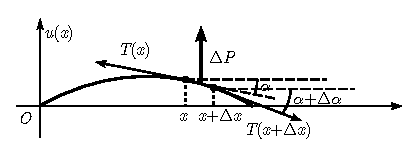
\includegraphics[scale=1]{string1.eps}
	\caption{Провисання $u(x)$ гнучкої струни у результаті дії розподіленого на $x\in(0, 1)$ навантаження $f(x)$.}\label{figstring}
\end{figure}

\textbf{Розв'язування.}

Розгляньмо рівновагу довільного елемента струни довжиною $\Delta \ell$. Проектуючи сили, які діють на вирізаний зі струни елемент, на вісі $Ox$, $Oy$ (Рис. \ref{figstring}), отримуємо рівняння
\[
-T(x)\cos \alpha(x) + T(x + \Delta x)\cos \alpha(x + \Delta x) = 0,
\]
\[
-T(x) \sin\alpha(x) + T(x + \Delta x) \sin\alpha(x + \Delta x) - \Delta P = 0,
\]
де $T(x)$ -- величина натягу струни у перерізі $x$, $\alpha(x)$ -- кут між дотичною до струни і віссю $Ox$, $\Delta P$ -- величина розподіленого навантаження, що припадає на вирізаний елемент.

З першого рівняння слідує, що $T(x) \cos \alpha(x) = T_0 = \textrm{const}$, тобто горизонтальна складова натягу струни завжди має стале значення. З другого рівняння знаходимо, що
\[
\mathrm{d}\left(T(x) \sin\alpha(x)\right) = \mathrm{d}P(x),
\]
або
\begin{equation}\label{strelong}
T_0\mathrm{d}\left(\tg \alpha(x)\right) = \mathrm{d} P(x), T_0 \mathrm{d}u' = \mathrm{d}P(x).
\end{equation}
У цій задачі $\mathrm{d}P(x) = f(x) \mathrm{d}x$. Поділивши обидві частини рівняння \eqref{strelong} на $\mathrm{d}x$, отримаємо базове звичайне диференціальне рівняння для провисання $u(x)$:
\begin{equation}\label{1710}
\displaystyle \frac{\mathrm{d}^{2}u}{\mathrm{d}x^{2}}=f(x)\textrm{ для }x\in(0,1)
\end{equation}
із граничними умовами
\begin{equation}\label{1711}
u(0)=0\textrm{ і }u(1)=0.
\end{equation}

Помножимо тепер, формально, обидві частини рівняння \eqref{1710} на $g(x, x')$ і проінтегруємо від $0$ до $1$ за змінною $x$. Матимемо
$$
\int_{0}^{1}g(x, x')\frac{\mathrm{d}^{2}u}{\mathrm{d}x^{2}}\mathrm{d}x=\int_{0}^{1}g(x, x')f(x)\mathrm{d}x.
$$
Ліву частину рівняння двічі проінтегруємо частинами:
\begin{equation}\label{1712}
\begin{array}{ll}
&\displaystyle\int_{0}^{1}\dfrac{\mathrm{d}^{2}}{\mathrm{d}x^{2}}g(x, x')u(x)\mathrm{d}x +\\
&+\left[g(1, x')\left.\dfrac{\mathrm{d}u}{\mathrm{d}x}\right|_{x=1}-g(0,x')\left.\dfrac{\mathrm{d}u}{\mathrm{d}x}\right|_{x=0}-u(1)\dfrac{\mathrm{d}g(1,x')}{\mathrm{d}x}+u(0)\dfrac{\mathrm{d}g(0,x')}{\mathrm{d}x}\right]=\\
&=\displaystyle\int_{0}^{1}g(x, x')f(x)\mathrm{d}x.
\end{array}
\end{equation}

Доданки у лівій частині рівняння \eqref{1712}, які взято у квадратні дужки, є доданками граничних умов. Врахування граничних умов \eqref{1711} призводить до рівності нулеві останніх двох доданків у лівій частині. Далі, очевидним вибором граничних умов для $g(x, x')$ буде такий
\begin{equation}\label{1713}
g(0,x')=0 \textrm{ і }g(1,x')=0.
\end{equation}

Вибравши умови таким чином, ми прибираємо взагалі усі доданки граничних умов (очевидно, так можна зробити далеко не у кожній задачі). Тепер припустімо, що $g(x, x')$ задовольняє рівняння
\begin{equation}\label{1714}
\frac{\mathrm{d}^{2}g(x,x')}{\mathrm{d}x^{2}}=\delta(x-x'),
\end{equation}
із граничними умовами \eqref{1713}. Підставивши значення функцій з рівнянь \eqref{1714} і \eqref{1713} до рівняння \eqref{1712}, матимемо розв'язок у такому вигляді:
\begin{equation}\label{1715}
u(x')=\int_{0}^{1}g(x, x')f(x)\mathrm{d}x.
\end{equation}

Для того щоб скористатися записаним розв'язком, достатньо лише знайти $g(x, x')$. Зауважимо, що якщо позначити диференціальний оператор $\mathrm{d}^{2}/\mathrm{d}x^{2}$ у початковому рівнянні через $L$, спряженим до нього оператором $L^{*}$ буде також $\mathrm{d}^{2}/\mathrm{d}x^{2}$, у чому неважко переконатися подвійним інтегруванням частинами. Таким чином, цей оператор є самоспряженим.

Останнім кроком у розв'язанні є визначення розв'язку \eqref{1714} із граничними умовами \eqref{1713}. Роль змінної тепер грає $x'$. Зафіксувавши якесь $x'$ із проміжку від $0$ до $1$, рівняння \eqref{1714} можна розв'язати окремо для проміжків $0<x<x'$ і $x'<x<1$. Маємо
\begin{subequations}
	\begin{align}
	&\displaystyle \frac{d^{2}g(x,x')}{\mathrm{d}x^{2}}=0\textrm{ для }0<x<x',\\
	&\displaystyle \frac{\mathrm{d}^{2}g(x,x')}{\mathrm{d}x^{2}}=0\textrm{ для }x'<x<1.
	\end{align}
\end{subequations}

Загальний розв'язок для кожного з підвідрізків визначається дуже просто:
\begin{subequations}\label{1717}
	\begin{align}
	&g(x, x')=Ax+B\textrm{ для }0<x<x'\label{1717a}\\
	&g(x, x')=Cx+D\textrm{ для }x'<x<1.\label{1717b}
	\end{align}
\end{subequations}

До цього загального розв'язку входить чотири невідомі сталі: $A$, $B$, $C$ і $D$. Два співвідношення для визначення цих сталих можна отримати з граничних умов \eqref{1713}.

Маємо
\begin{equation}\label{1718}
g(0, x')=0\to  B=0;\quad g(1, x')=0\to  C+D=0.
\end{equation}

Щоб отримати ще два співвідношення, потрібні для визначення усіх чотирьох сталих, повернемося до основного рівняння \eqref{1714}. Проінтегруємо його обидві частини за $x$ від $x'-\varepsilon$ до $x'+\varepsilon$ і перейдемо до границі $\varepsilon\to  0$. Дістанемо
$$
\lim_{\varepsilon\to 0}\displaystyle\int_{x'-\varepsilon}^{x'+\varepsilon}\frac{\mathrm{d}^{2}g(x,x')}{\mathrm{d}x^{2}}\mathrm{d}x = \lim_{\varepsilon\to 0}\displaystyle\int_{x'-\varepsilon}^{x'+\varepsilon}\delta(x-x') \mathrm{d}x,
$$
звідки
\begin{equation}\label{1719}
\left.\dfrac{\mathrm{d}g(x,x')}{\mathrm{d}x}\right|_{x=x'^{+}}-\left.\dfrac{\mathrm{d}g(x,x')}{\mathrm{d}x}\right|_{x=x'^{-}}=1.
\end{equation}

Таким чином, перша похідна від $g(x, x')$ має розрив першого роду при переході $x$ через $x'$. Втім, як можна сподіватися, сама $g(x, x')$ має бути неперервною у $x'$, тобто
\begin{equation}\label{1720}
\left.g(x, x')\right|_{x=x'^{+}}=\left.g(x, x')\right|_{x=x'^{-}}.
\end{equation}

Вище, через $x'^{+}$ і $x'^{-}$ позначено точки, які є нескінченно близькими до $x'$ праворуч і ліворуч відповідно. Використовуючи розв'язки \eqref{1717a} і \eqref{1717b} для $g(x, x')$ на кожному з підвідрізків, знаходимо, відповідно, з рівнянь \eqref{1719} і \eqref{1720}
\begin{equation}\label{1721}
C-A=1, Cx'+D=Ax'+B.
\end{equation}

Рівняннями \eqref{1718} і \eqref{1721} можна скористатися для визначення усіх чотирьох сталих $A$, $B$, $C$ і $D$:
$$
A=x'-1, B=0, C=x', D=-x',
$$
звідки розв'язок \eqref{1717} набуває форми
\begin{subequations}\label{1722}
	\begin{align}
	g(x, x')&=\left\{\begin{array}{lll}
	(x'-1)x&\textrm{для}&x<x',\\
	x'(x-1)&\textrm{для}&x>x',
	\end{array}\right.\\
	&=x_{<}(x_{>}-1) \textrm{ для }\left\{\begin{array}{lll}x_{<} &=& (x+x')/2-|x+x'|/2,\\
	x_{<} &=& (x+x')/2+|x+x'|/2.\end{array}\right.
	\end{align}
\end{subequations}

Фізично, функція Ґріна \eqref{1722} відповідає провисанню струни під дією \emph{зосередженого навантаження} $\delta(x-x')$, прикладеного у точці $x=x'$, як це показано на Рис. \ref{figstring2}. Через це цю функцію також називають \emph{функцією впливу}\index{функція!впливу}.

\begin{figure}[ht]\centering
	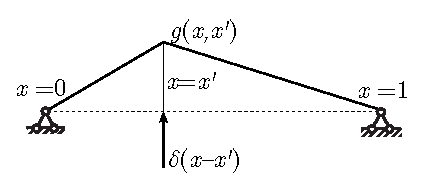
\includegraphics[scale=1]{string2.eps}
	\caption{Провисання $u(x)$ гнучкої струни під дією зосередженого навантаження $\delta(x-x')$, прикладеного у точці $x=x'$.}\label{figstring2}
\end{figure}

Знайдену нами функцію впливу для зосередженої сили можна тепер використати для розв'язування задачі для будь-якого розподіленого навантаження $f(x)$ за допомогою рівняння \eqref{1715}:
\begin{equation}
\begin{array}{lll}
u(x)&=&\displaystyle\int_{0}^{1}g(\xi, x)f(\xi)\mathrm{d}\xi=\\
&=&\displaystyle \int_{0}^{x} (x-1)\xi f(\xi)\mathrm{d}\xi+\int_{x}^{1}x(\xi -1 )f(\xi)\mathrm{d}\xi =\\
&=&(x-1)\displaystyle\int_{0}^{x}\xi f(\xi)\mathrm{d}\xi+x\displaystyle\int_{x}^{1}(\xi-1)f(\xi)\mathrm{d}\xi.
\end{array}
\end{equation}

\section{Складніший приклад застосування функцій Ґріна. Рівняння Сомільяни}

Теорема Бетті:
\begin{equation}
\sigma_{ij}\varepsilon'_{ij}=\sigma'_{ij}\varepsilon_{ij}
\end{equation}

Інтегральна форма:
\begin{equation}
\begin{array}{lll}
\displaystyle\int_{V} \sigma_{ij}\varepsilon'_{ij} \mathrm{d}V &=& \dfrac{1}{2} \displaystyle\int_{V} \sigma_{ij}\left(u'_{i,j} + u'_{j,i}\right)\mathrm{d}V=\displaystyle\int_{V} \sigma_{ij} u'_{i,j} \mathrm{d}V =\displaystyle\int_{S} \sigma_{ij}n_ju'_{i} \mathrm{d}S -\\
&-& \displaystyle\int_{V} \sigma_{ij,j} u_{i} \mathrm{d}V = \displaystyle\int_{S} p_{i} u'_{i} \mathrm{d}S + \int_{V} X_{i}u'_{i} \mathrm{d}V= \displaystyle\int_{S} p'_{i} u_{i} \mathrm{d}S + \displaystyle\int_{V} X'_{i}u_{i} \mathrm{d}V
\end{array}
\end{equation}

\begin{equation}
\Delta u=f; \Delta E(x,\xi)=\delta(x-\xi);
\end{equation}

\begin{equation}
u(x)=\displaystyle\int_{V} f(\xi) E(x,\xi)\mathrm{d}V + \displaystyle\int_{S} \dfrac{\partial u}{\partial n} \mathrm{d}S - \displaystyle\int_{S} u \dfrac{\partial E}{\partial n} \mathrm{d}S.
\end{equation}
$E(x,\xi)$ -- фундаментальний розв'язок (реакція нескінченного тіла на дію точкового навантаження).

\begin{equation}
\displaystyle\int_{S} p_{i} u'_{i} \mathrm{d}S + \int_{V} X_{i}u'_{i} \mathrm{d}V= \displaystyle\int_{S} p'_{i} u_{i} \mathrm{d}S + \displaystyle\int_{V} X'_{i}u_{i} \mathrm{d}V
\end{equation}
покладемо $X'_{i} = \delta_{ik}\delta(x-\xi)$. Тобто у $\xi$ розташуємо одиничну силу у напрямку $x_k$.

Ця сила викличе у $x$ переміщення $U_{i}^{k} (x,\xi)$ у напрямку $x_i$. $U_{i}^{k}(x, \xi)$ задовольняють такі рівняння:

\begin{equation}
(\lambda + \mu) u_{l,li}^{k} + \mu u_{i,ll}^{k} + \delta_{ik}\delta(x-\xi) = 0.
\end{equation}
$U_i^k$ -- система фундаментальних розв'язків (функцій Ґріна) рівнянь у переміщеннях для однорідного тіла.

Для збереження рівноваги тіла слід вибрати $p'_{i}$ особливим чином:
\begin{equation}
p'_I(x, \xi) \left(\lambda U_{l,l}^k \delta_{ij} + \mu (U_{i,j}^k + U_{j,i})\right)n_j = q_i^k (x, \xi).
\end{equation}

Для теореми Бетті:
\begin{equation}
X'_i = \delta_{ik} \delta(x-\xi); p'_i = q_i^k(x, \xi); u'_i = U_i^k(x, \xi).
\end{equation}

Тоді
\begin{equation}
\displaystyle\int_{S} p_{i} U_i^k (x, \xi)\mathrm{d}S_x + \int_{V} X_{i}U_i^k (x, \xi) \mathrm{d}V_x= \displaystyle\int_{S} q_i^k (x, \xi) u_{i} \mathrm{d}S_x + \displaystyle\int_{V} \delta_{ik} \delta(x-\xi) X'_{i}u_{i} \mathrm{d}V_x
\end{equation}

\begin{equation}
\displaystyle\int_{V} \delta_{ik} \delta(x-\xi) X'_{i}u_{i} \mathrm{d}V_x=\left\{
\begin{array}{lll}
u_k(\xi), &\xi& \in V;\\
0, &\xi& \notin V.
\end{array}
\right.
\end{equation}

Отже, якщо $\xi \in V$,
\begin{equation}\label{som1}
u_k(\xi) = \int_{V} X_{i}U_i^k (x, \xi) \mathrm{d}V_x + \displaystyle\int_{S} p_{i} U_i^k (x, \xi)\mathrm{d}S_x - \displaystyle\int_{S} q_i^k (x, \xi) u_{i} \mathrm{d}S_x.
\end{equation}

Якщо ж $\xi \notin V$,
\begin{equation}\label{som2}
\int_{V} X_{i}U_i^k (x, \xi) \mathrm{d}V_x + \displaystyle\int_{S} p_{i} U_i^k (x, \xi)\mathrm{d}S_x - \displaystyle\int_{S} q_i^k (x, \xi) u_{i} \mathrm{d}S_x=0.
\end{equation}

Рівняння \eqref{som1} і \eqref{som2} називаються рівняннями Сомільяни\footnote{Carlo Somigliana (1860 -- 1955) -- італійський математик}.

$\displaystyle\int_{V} X_{i}U_i^k (x, \xi) \mathrm{d}V_x$ -- ньютонів потенціал.

$\displaystyle\int_{S} p_{i} U_i^k (x, \xi)\mathrm{d}S_x$ -- потенціал простого шару.

$\displaystyle\int_{S} q_i^k (x, \xi) u_{i} \mathrm{d}S_x$ -- потенціал подвійного шару.

\chapter{Поняття про коректно поставлені задачі. Інтегральне рівняння Фредгольма першого роду як некоректно поставлена задача}\label{fred1sec}

Розв'язання інтегрального рівняння Фредгольма 1-го роду
\begin{equation}\label{fred1kind}
\int_{a}^{b} K(t, s) \varphi(s)\mathrm{d}s = f(t),
\end{equation}
де $K(t, s)$, $f(t)$ -- відомі функції, $\varphi(t)$ -- шукана функція, пов'язане із специфічними труднощами, суттєво відмінними від тих, з якими можна зустрітися у теорії інтегральних рівнянь 2-го роду.

Нехай, наприклад, ядро $K(t, s)$ є поліном відносно $t$ та $s$:
\[
K(t, s) = a_0(s) t^m + a_1(s)t^{m-1} + \ldots + a_m(s),
\]
де $a_i(s)$ -- поліноми відносно $s$ ($i = \overline{1, m}$).

Тоді ліва частина \eqref{fred1kind} буде мати вигляд $b_0 t^m + b_1t^{m-1} + \ldots  + b_m$ для будь-якої функції $\varphi(t) \in \cab$, а отже, такий саме вигляд повинна мати і права частина \eqref{fred1kind}, тобто функція $f(t)$.

Таким чином, для будь-якої неперервної функції $f(t)$ розв'язок рівняння \eqref{fred1kind}, загалом кажучи, не існує при як завгодно <<доброму>> ядрі $K(t, s)$.

Далі, розгляньмо, наприклад, найпростіше інтегральне рівняння 1-го роду
\[
\int_{0}^{1} \varphi(s) \mathrm{d}s = t
\]
з ядром $K(t, s) \equiv 1$ і $f(t) = t$.

Очевидно, що у класі інтегровних (зокрема, неперервних) функцій це рівняння не має розв'язків.

Нехай ядро $K(t, s)$ рівняння \eqref{fred1kind} симетричне.

Внаслідок теореми Гільберта -- Шмідта для існування розв'язку рівняння \eqref{fred1kind} необхідно, щоб функція $f(t)$ розкладалася за власними функціями $\{\varphi_i(t)\}$ ядра $K(t, s)$:
\begin{equation}\label{ftexp}
 f(t) = \sum_{i} (f, \varphi_i) \varphi_i(t).
\end{equation}

За виконання цієї умови, розв'язок $\varphi(t)$ рівняння \eqref{fred1kind} можна шукати у вигляді
\begin{equation}\label{varphii}
 \varphi(t) = \sum_{i} c_i \varphi_i(t).
\end{equation}
Підставляючи \eqref{varphii} до \eqref{fred1kind} і порівнюючи з \eqref{ftexp}, одержимо $\dfrac{c_i}{\lambda_i} = (f, \varphi_i)$, звідки. $c_i = \lambda_i (f, \varphi_i)$. Якщо нам потрібно, щоб розв'язок $\varphi(t)$ належав до $L_2([a; b])$, слід накласти на $f(t)$ додаткові вимоги (умови теореми Пікара\footnote{Charles \'{E}mile Picard (1856 -- 1941) -- французький математик, відомий дослідженнями у широкому колі математичних проблем.}).

\begin{thm}[Пікар]
Інтегральне рівняння 1-го роду із замкненим симетричним\footnote{Симетричне ядро $K(t, s)$ називається замкненим в $L_2([a; b])$, якщо кожна функція $\omega(t) \in L_2([a; b])$, що задовольняє тотожність
\[
 \int_{a}^{b} K(t, s) \omega(s) \mathrm{d}s = 0,
\]
рівна нулю майже всюди на $[a; b]$\index{ядро!замкнене}. Замкнене ядро характеризується тим, що власні функції ядра утворюють повну в $L_2([a; b])$ ортогональну систему функцій.} ядром $K(t, s)$ \eqref{fred1kind}, де $f(t) \in L_2([a; b])$, має, і при тому єдиний, розв'язок у класі $L_2([a; b])$ тоді й лише тоді, коли ряд
\begin{equation}\label{lfseries}
 \sum_{k=1}^{\infty} \lambda_k^2 f_k^2
\end{equation}
збіжний.

Тут $\lambda_k$ -- характеристичні числа ядра $K(t, s)$, $f_k = (f, \varphi_k)$ -- коефіцієнти Фур'є функції $f(t)$ щодо власних функцій $\varphi_n(t)$ цього ядра:
\begin{equation}
 \varphi_n(t) = \lambda_n \int_{a}^{b} K(t, s) \varphi_n(s) \mathrm{d}s.
\end{equation}
\end{thm}

\begin{proof}
Припустімо, що існує розв'язок $\varphi(t) \in L_2([a; b])$ рівняння \eqref{fred1kind}. Тоді матимемо
\begin{multline}\label{fneq}
 f_n = \int_{a}^{b} f(t) \varphi_n(t) \mathrm{d}t = \int_{a}^{b} \left\{\int_{a}^{b} K(t, s) \varphi(s) \mathrm{d}s\right\}\varphi_n(t) \mathrm{d}t=\\
=\int_{a}^{b} \left\{\int_{a}^{b} K(t, s) \varphi_n(t) \mathrm{d}t\right\}\varphi(t) \mathrm{d}s = \frac{1}{\lambda_n} \int_{a}^{b} \varphi_n(s) \varphi(s) \mathrm{d}s.
\end{multline}
Тут ми скористалися тим, що внаслідок \eqref{fred1kind}
\[
 f(t) = \int_{a}^{b} K(t, s) \varphi(s) \mathrm{d}s,
\]
а також тим, що внаслідок симетричності ядра
\[
 \int_{a}^{b} K(t, s) \varphi_n(t) \mathrm{d}t = \frac{1}{\lambda_n} \varphi_n(s).
\]

Рівність \eqref{fneq} можна записати у вигляді
\begin{equation}\label{intlf}
 \int_{a}^{b} \varphi(s) \varphi_n(s) \mathrm{d}s = \lambda_n f_n,
\end{equation}
звідки видно, що числа $\lambda_n f_n$ є коефіцієнтами Фур'є функції $\varphi(t) \in L_2([a; b])$. Як відомо, ряд \eqref{lfseries}, що складається з квадратів таких коефіцієнтів, обов'язково має бути збіжним.

Припустімо, навпаки, що ряд \eqref{lfseries} збігається. Тоді через ізометричність і ізоморфність просторів $L_2([a; b])$ і $l_2$ (теорема Ріса-Фішера \cite{Sobolev}) існує функція $\varphi(t) \in L_2([a; b])$, і при тому єдина, для якої числа $\lambda_n f_n$ є коефіцієнтами Фур'є за системою функцій $\{\varphi_n(t)\}$, тобто виконуються рівності \eqref{intlf} для усіх $n$ ($n \in \mathbb{N}$). Ця функція $\varphi(t)$ задовольняє дане інтегральне рівняння. Справді, за побудовою $\varphi(t)$, функції $f(t)$ і $\int_{a}^{b} K(t, s) \varphi(s) \mathrm{d}s$ коефіцієнти Фур'є щодо системи системи $\{\varphi_n(t)\}$ власних функцій ядра $K(t, s)$ у цих функцій є однаковими.

Отже, функції $f(t)$ і $\int_{a}^{b} K(t, s) \varphi(s) \mathrm{d}s$ тотожні (у сенсі метрики $L_2([a; b])$).
\end{proof}

Якщо ядро $K(t, s)$ не є замкненим, то розв'язок рівняння \eqref{fred1kind} не єдиний. Нехай $\omega_1(t)$, \ldots, $\omega_k(t)$ -- не рівні нулю майже всюди функції такі, що
\[
 \int_{a}^{b} K(t, s) \omega_j(s) \mathrm{d}s = 0 \quad (j = \overline{1, k}).
\]

Тоді, якщо $\varphi_0(t)$ -- розв'язок рівняння \eqref{fred1kind}, то функція
\[
 \varphi_0(t) + \sum_{j=1}^{k} C_j \omega_j(t),
\]
де $C_j$ ($j = \overline{1, k}$) -- довільні сталі, також буде розв'язком цього рівняння. У випадку виродженого ядра розв'язок рівняння \eqref{fred1kind} може містити нескінченну кількість довільних сталих.

Вимога замкненості ядра $K(t, s)$ є істотною не лише для єдиності розв'язку рівняння \eqref{fred1kind}, але й взагалі для можливості розв'язання цього рівняння. Якщо відмовитися від вимоги замкненості, то серед рівнянь вигляду
\[
 \int_{a}^{b} K(t, s) \varphi(s) \mathrm{d}s = f(t) + g(t),
\]
де $f(t)$ -- задана неперервна функція, не ортогональна до усіх $\varphi_n(t)$, a $g(t)$ -- будь-яка неперервна функція, ортогональна до всіх $\varphi_n(t)$, можна знайти нерозв'язні рівняння.

Розгляньмо, наприклад, рівняння
\begin{equation}\label{simplefred1}
 \int_{0}^{1} \varphi(s) \mathrm{d}s = 1.
\end{equation}

Воно має очевидний розв'язок $\varphi(t) \equiv 1$. Безпосередньою перевіркою переконуємося у тому, що розв'язками рівняння \eqref{simplefred1} будуть також функції
\[
 \varphi(t) = 1 + \omega(t),
\]
де $\omega(t) = \alpha t + \beta$ і величини $\alpha$, $\beta$ -- будь-які дійсні числа, що задовольняють умову $\alpha + 2 \beta =0$.

З іншого боку, рівняння
\[
 \int_{0}^{1} \varphi(s) \mathrm{d}s = 1 + t,
\]
очевидно, нерозв'язне.

Для розв'язання деяких інтегральних рівнянь Фредгольма 1-го роду можна застосовувати метод послідовних наближень.
\begin{thm}
 Нехай $K(t, s)$ -- симетричне додатно визначене $L_2$-ядро, і нехай рівняння
 \eqref{fred1kind} однозначно розв'язне.

Тоді послідовність $\{\varphi_n(t)\}$, визначена рекурентним співвідношенням
\begin{equation}\label{iterfred1}
 \varphi_n(t) = \varphi_{n-1}(t) + \lambda \left[f(t) - \int_{a}^{b} K(t, s) \varphi_{n-1}(s) \mathrm{d}s \right], \quad n\in \mathbb{N},
\end{equation}
де
\begin{equation}
 \varphi_0(t) \in L_2([a; b]), 0<\lambda < 2 \lambda_1
\end{equation}
і $\lambda_1$ -- найменше характеристичне число ядра $K(t, s)$, збігається у середньому до розв'язку рівняння \eqref{fred1kind}.
\end{thm}

\begin{proof}
Справді, покладаючи у рівності \eqref{iterfred1}
\[
 \varphi_n(t) = \varphi(t) + u_n(t),
\]
надамо їй вигляду
\begin{equation}\label{uiter}
 u_n(t) = u_{n-1}(t) + \lambda \int_{a}^{b} K(t, s) u_{n-1}(s) \mathrm{d}s.
\end{equation}

Помножимо обидві частини \eqref{uiter} на власну функцію $v_i(t)$ ядра й проінтегруємо за $t$ від $a$ до $b$. Дістанемо
\begin{equation}\label{alphain}
 \alpha_i^n = \alpha_i^{n-1} - \lambda \int_{a}^{b} v_i(t) \mathrm{d}t \int_{a}^{b} K(t, s) u_{n-1}(s) \mathrm{d}s,
\end{equation}
де
\[
 \alpha_i^n = \int_{a}^{b} u_n(t) v_i(t) \mathrm{d}t.
\]

Використовуючи симетричність ядра $K(t, s)$ і те, що
\[
 v_i(t) = \lambda_i \int_{a}^{b} K(t, s) v_i(s) \mathrm{d}s,
\]
отримаємо
\[
 \int_{a}^{b} v_i(t) \mathrm{d}t \int_{a}^{b} K(t, s) u_{n-1}(s) \mathrm{d}s = \frac{\alpha_i^{n-1}}{\lambda_i}.
\]

Таким чином, з \eqref{alphain}
\[
 \alpha_i^n = \left(1 - \frac{\lambda}{\lambda_i}\right) \alpha_i^{n-1} = \left(1 - \frac{\lambda}{\lambda_i}\right)^n \alpha_i^0.
\]

Розгляньмо інтеграл
\[
 \int_{a}^{b} u_n^2(t)\mathrm{d}t = \int_{a}^{b} [\varphi_n(t) - \varphi(t)]^2 \mathrm{d}t.
\]

Внаслідок повноти системи функцій $\{v_i(t)\}$ маємо
\[
 \int_{a}^{b} u_n^2(t) \mathrm{d}t = \sum_{i=1}^{\infty} (\alpha_i^n)^2 = \sum_{i=1}^{\infty} \left(1-\frac{\lambda}{\lambda_i}\right)^{2n} (\alpha_i^0)^2.
\]

Оскільки $0<\lambda < 2 \lambda_1$,
\[
 \left(1 - \frac{\lambda}{\lambda_i}\right)^2 \leqslant 1.
\]
Тому для будь-якого $\varepsilon > 0$ можна вказати такий номер $N = N(\varepsilon)$, що при $n > N(\varepsilon)$
\[
 \sum_{i=1}^{\infty} \left(\alpha_i^n\right)^2 < \varepsilon.
\]
Таким чином, ми отримуємо нерівність
\[
 \int_{a}^{b} u_n^2(t) \mathrm{d}t = \int_{a}^{b} \left[\varphi_n(t) - \varphi(t)\right]^2 \mathrm{d}t < \varepsilon,
\]
яка означає, що послідовність $\{\varphi_n(t)\}$ збігається у середньому до розв'язку $\varphi(t)$ рівняння \eqref{fred1kind}.
\end{proof}

Знову розгляньмо рівняння \eqref{fred1kind}, не припускаючи тепер, що ядро є симетричним. Застосуємо до його розв'язування загальний метод невизначених коефіцієнтів. Суть цього методу -- розкладення шуканої функції за деякою повною системою функцій. Він виявляється, взагалі, добре пристосованим до розв'язування інтегральних рівнянь Фредгольма 1-го роду.

Будемо шукати розв'язок $\varphi(t)$ рівняння \eqref{fred1kind} у вигляді
\begin{equation}\label{decompsolfred1}
 \varphi(t) = \sum_{n} a_n g_n(t) w(t),
\end{equation}
де функції $g_n(t)$ ($n \in \mathbb{N}$)) утворюють деякі повну систему на інтервалі $(a, b)$; $w(t)$ -- деяка вагова функція, яку слід вибирати близькою до $\varphi(t)$ і тим самим поліпшити збіжність ряду \eqref{decompsolfred1}. Якщо про розв'язок $\varphi(t)$ немає ніяких відомостей, можна покласти $w(t) = 1$.

Підставляючи $\varphi(t)$ у формі \eqref{decompsolfred1} у рівняння \eqref{fred1kind}, матимемо
\[
 f(t) = \sum_n a_n \int_{a}^{b} K(t, s) g_n(s) w(s) \mathrm{d}s,
\]
або
\begin{equation}\label{fexpdecomp}
 f(t) = \sum_n a_n h_n(t),
\end{equation}
де $h_n(t)$ -- відомі функції:
\begin{equation}
 h_n(t) = \int_{a}^{b} K(t, s) g_n(s) w(s) \mathrm{d}s.
\end{equation}

Таким чином, розв'язання інтегрального рівняння зведеться до знаходження коефіцієнтів $a_n$ за відомими функціями $f(t)$ і $h_n(t)$.

Особливо просто це зробити у двох випадках:

1) Якщо функції $h_n(t) = c_n t^n$ ($n= 0, 1, \ldots$), то права частина \eqref{fexpdecomp} виявляється степеневим рядом, отже невідомі коефіцієнти $a_n$ можна визначити шляхом порівняння коефіцієнтів цього ряду із відповідними коефіцієнтами у розкладі $f(t)$ за степенями $t$.

2) Якщо функції $h_n(t)$ утворюють ортогональне з вагою $\rho(t)$ сімейство на інтервалі $(a, b)$:
\[
 \int_{a}^{b} \rho h_n(t) h_m(t) \mathrm{d}t = N\delta_{mn}.
\]

Тут $\delta_{mn}$ -- символ Кронекера,
\[
 \delta_{mn} = \left\{
\begin{array}{lll}
 0, &\textrm{якщо}& m \neq n,\\
 1, &\textrm{якщо}& m = n.
\end{array}
\right.
\]

Тобто коефіцієнти $a_n$ легко визначаються з \eqref{fexpdecomp} за формулами
\[
 a_n = \frac{1}{N_n} \int_{a}^{b} f(t) \rho(t) h_n(t) \mathrm{d}t,
\]
де
\[
 N_n = \int_{a}^{b} \rho(t) h_n^2(t) \mathrm{d}t.
\]

На жаль, загалом, функції $h_n(t)$ не є ні степенями $t$, ні елементами ортогональної системи і визначення коефіцієнтів $a_n$ буває пов'язане зі значними технічними труднощами.

Як приклад, що ілюструє викладений метод, розгляньмо випадок $h_n(t) = t^n$.

Такий випадок має місце, коли ядро інтегрального рівняння є твірною функцією для сімейства ортогональних поліномів.

\begin{dfn}
Функція $G(t, z)$ називається твірною\index{твірна системи функцій} для системи функцій
\[
 g_0(z), g_1(z), \ldots, g_n(z), \ldots
\]
якщо
\[
 G(t, z) = \sum_{n=0}^{\infty} c_n g_n(z) t^n \quad (c_n \neq 0),
\]
тобто якщо функції $g_n(z)$ ($n = 0, 1, 2, \ldots$) отримуються у результаті розкладання $G(t, z)$ у ряд за степенями $t$.
\end{dfn}

Як відомо, твірну функцію для поліномів Ерміта $H_n(z)$ можна записати у вигляді
\begin{equation}\label{hermiteexp}
 e^{-(t-z)^2} = \sum_{n=0}^{\infty} \frac{e^{-z^2} H_n(z)}{n!} t^n.
\end{equation}

Цей розклад можна застосувати для розв'язування інтегрального рівняння
\begin{equation}\label{hermexeq}
 f(t) = \int_{-\infty}^{+\infty} e^{-(t-s)^2} \varphi(s) \mathrm{d}s.
\end{equation}

Задачі такого типу виникають у питаннях про поширення тепла, коли шуканим є первісний розподіл джерел, який породжує деякий заданий розподіл температури. Покладемо
\[
 \varphi(s) = \sum_n a_n H_n(s).
\]

Використовуючи розклад \eqref{hermiteexp} ядра рівняння \eqref{hermexeq} і той факт, що
\[
 \int_{-\infty}^{+\infty} H_n^2(s) e^{-s^2} \mathrm{d}s = 2^n n! \sqrt{\pi},
\]
Можемо звести рівняння \eqref{hermexeq} до вигляду
\[
 f(t) = \sqrt{\pi} \sum_n a_n 2^n t^n.
\]
Звідси
\[
 a_n = \frac{f^{(n)}(0)}{2^n n! \sqrt{\pi}}.
\]
А отже, розв'язок $\varphi(t)$ рівняння \eqref{hermexeq} має вигляд
\[
 \varphi(t) = \frac{1}{\sqrt{\pi}} \sum _n \frac{f^{(n)}(0)}{2^n n!} H_n(t).
\]


\section{Операторні рівняння 1-го роду. Поняття регуляризації}

Розгляньмо операторне рівняння
\begin{equation}\label{illopeq}
Ax=f
\end{equation}
Тут $A:X\to  Y$ є лінійним оператором, що діє з нормованого лінійного простору $X$ до нормованого лінійного простору $Y$.
\begin{dfn}
	Операторне рівняння \eqref{illopeq} називається некоректним, якщо оператор $A$ не задовольняє хоча б одну з таких умов:
	\begin{itemize}
		\item $A$ є бієкцією;
		\item оператор $A^{-1}: Y\to  X$, якщо він існує, є неперервним.
	\end{itemize}
\end{dfn}

Дамо одне означення, яке буде корисним для формалізації вимог до оператора $A$, які визначають множину некоректних задач для рівняння \eqref{illopeq}.

\begin{dfn}
	Лінійний оператор $A:X\to  Y$ називають обмеженим знизу, якщо існує таке $C>0$, що $\|Ax\| \geqslant C\|x\|$, $\forall x \in X$.
\end{dfn}

Результати досліджень у межах функціонального аналізу показують, що \eqref{illopeq} є некоректним тоді й лише тоді, коли або $T$ не є сюр'єкцією або не є обмеженим знизу.

Якщо $A$ не є сюр'єкцією, тоді існують $f\in Y$ такі, що \eqref{illopeq} є нерозв'язним. У таких випадках доводиться шукати так званий \emph{розв'язок із мінімальною нормою лишку}, скажімо $\hat{x}$. Якщо існування такого $\hat{x}$ гарантовано, варто визначити умови, за яких задача визначення $\hat{x}$ є коректною. Якщо модифікована задача також некоректна, доводиться її \emph{регуляризувати}.

\begin{dfn}
	Регуляризацією\index{регуляризація} рівняння \eqref{illopeq} називається заміна початкової некоректної задачі сімейством \emph{близьких до неї} коректних задач і наступне наближення до $\hat{x}$ із прямуванням похибки у даних $а$ до нуля.
\end{dfn}

Наведемо приклад некоректності \eqref{illopeq}, коли $A$ не обмежено знизу.

Нехай $A$ не є обмеженим знизу. Тоді, для будь-якого $n\in \mathbb{N}$, існує ненульове $u_n \in X$ таке, що $\Vert Au_{n}\Vert<(1/n)\Vert u_{n}\Vert$ для усіх $n\in \mathbb{N}$. Отже, якщо $x\in X$ і $x_{n} :=x+\sqrt{n}u_{n}/\|u_{n}\|$ тоді
$$
\Vert Ax_{n}-Ax\Vert=\frac{\sqrt{n}||Au_{n}\Vert}{\Vert u_{n}\Vert}<\frac{1}{\sqrt{n}}\xrightarrow{n\to\infty} 0,
$$
але
$$
\Vert x_{n}-x\Vert=\sqrt{n}\xrightarrow{n\to\infty}\infty.
$$

Прикладом операторного рівняння 1-го роду є інтегральне рівняння Фредгольма 1-го роду
\begin{equation}\label{fred1oncemore}
 \int_{a}^{b} K(t, s) \varphi(s) \mathrm{d}s = f(t),
\end{equation}
де $K(t, s)$ -- інтегроване із квадратом у прямокутнику $Q=\{a \leqslant t, s \leqslant b\}$ ядро, а $\varphi(t)$ і $f(t)$ -- функції з $L_2([a; b])$ є прикладом операторного рівняння 1-го роду.

Також некоректними є рівняння задачі, яка виникає під час аналізу даних геологорозвідки:
\[
 \gamma\int_{0}^{1} \dfrac{1}{[1+(t-s)^2]^{3/2}}\varphi(s)\mathrm{d}s = f(t), t\in[0;1],
\]
рівняння зворотної задачі теплопровідності:
\[
 \int_{0}^{\pi} K(t, s) \varphi(s)\mathrm{d}s = f(t), t\in\left[0; \pi\right],
\]
де
\[
 K(t,s) = \dfrac{2}{\pi} \sum\limits_{n=1}^{\infty} \sin nt \sin ns,
\]
рівняння задачі комп'ютерної томографії (рівняння Абеля першого роду):
\[
 \int_{s}^{R} \dfrac{2s\varphi(s)}{\sqrt{s^2-t^2}}\mathrm{d}s = f(t), t\in \left(0, R\right].
\]


Одним з істотних моментів у теорії таких рівнянь є те, що оператор, обернений до компактного, не обмежений. Тому, якщо $f_1$ і $f_2$ -- два близьких між собою елемента з $Y$ і обидва рівняння
\[
 A \varphi = f_1, \quad A \varphi = f_2
\]
розв'язні, то відповідні розв'язки $\varphi_1 = A^{-1} f_1$ і $\varphi_2 = A^{-1} f_2$ можуть значно відрізнятися один від одного.

Таким чином, як завгодно мала похибка у вільному члені рівняння \eqref{illopeq} може привести до як завгодно великої помилки у розв'язку.


Розгляньмо рівняння \eqref{illopeq}, де $A$ -- лінійний компактний оператор і $\|A\| \leqslant 1$.

Нехай задачу з розв'язання рівняння \eqref{illopeq} поставлено коректно, і нехай множина коректності $M$ є множиною функцій $u$, які визначаються співвідношенням
\begin{equation}\label{uebv}
 u = Bv, \quad \|v\| \leqslant 1,
\end{equation}
де $B$ -- лінійний компактний оператор, $\|B\| \leqslant 1$.

Нехай задана функція $\omega(\tau)$, що задовольняє наступні умови:

а) $\omega(\tau)$ -- неперервна неспадна функція, і $\omega(0) = 0$;

б) для будь-якого $u \in M$, що задовольняє нерівность
\[
 \|Au\| \leqslant \tau,
\]
має місце нерівність
\begin{equation}\label{ineqfred1plpl}
 \|u\| \leqslant \omega(\tau).
\end{equation}

Вкажемо один метод розв'язання рівняння \eqref{illopeq}, обмежившись найпростішим випадком.

Нехай $A$ -- додатно визначений симетричний оператор і оператори $A$ і $B$ можна переставляти. Позначимо через $\varphi_{\tau}$ функцію
\[
 \varphi_{\tau} = (A + \tau I)^{-1} f, \tau\geqslant 0,
\]
і оцінимо різницю $\varphi_{\tau} - \varphi$. Внаслідок \eqref{illopeq}, \eqref{uebv} маємо
\begin{equation}
 \varphi_{\tau} - \varphi = \left\{(A + \tau I)^{-1} A - I\right\} B\psi = - \tau B(A+\tau I)^{-1} \psi
\end{equation}
де $\varphi = B \psi$, $\|\psi\| \leqslant 1$.

Функція $w_{\tau} = \tau (A + \tau I)^{-1} \psi$ задовольняє нерівності
\begin{equation}\label{ineqfred1}
 \|w_{\tau}\| \leqslant 1, \|A w_{\tau} \| \leqslant \tau, \|AB w_{\tau}\| \leqslant \tau.
\end{equation}
Справді, внаслідок додатної визначеності оператора $A$, для будь-якої функції $w$ маємо
\begin{equation}\label{ineqfred1pl}
 \left.
 \begin{array}{r}
  \|(A + \tau I) w\| \geqslant \|Aw\|,\\
  \|(A + \tau I) w\| \geqslant \tau \|w\|,
 \end{array}
 \right\}
\end{equation}
звідки, взявши замість $w$ функцію $(A + \tau I)^{-1} w$, дістанемо
\begin{equation}\label{wineq}
 \left.
 \begin{array}{r}
  \|A(A + \tau I)^{-1} w\| \geqslant \|w\|,\\
  \|(A + \tau I)^{-1} w\| \geqslant \frac{1}{\tau} \|w\|,
 \end{array}
 \right\}
\end{equation}

З нерівностей \eqref{wineq} уже випливають нерівності \eqref{ineqfred1}. З нерівностей \eqref{ineqfred1pl} і з нерівності \eqref{ineqfred1plpl} отримуємо
\begin{equation}\label{bwineq}
 \|B w_{\tau} \| = \|\varphi_{\tau} - \varphi \| \leqslant \omega(\tau).
\end{equation}

Таким чином, якщо функція $f$ така, що рівняння \eqref{illopeq} розв'язне, то $\varphi_{\tau} \to \varphi$ за нормою при $\tau \to 0$.

Нехай тепер права частина $f$ відома з точністю до $\varepsilon$, тобто відома функція $f_{\varepsilon}$ така, що
\[
 \|f - f_{\varepsilon}\| < \varepsilon.
\]
Позначимо через $\varphi_{\tau\varepsilon}$ функцію
\[
 \varphi_{\tau\varepsilon} = (A + \tau I)^{-1} f_{\varepsilon}
\]
і оцінимо різницю $\varphi - \varphi_{\tau\varepsilon}$. Внаслідок \eqref{wineq} і \eqref{bwineq} маємо
\begin{equation}\label{varphite}
 \|\varphi - \varphi_{\tau\varepsilon} \| \leqslant \omega(\tau) + \|(A+\tau I)^{-1} (f - f_{\varepsilon})\| \leqslant \omega(\tau) + \varepsilon/\tau.
\end{equation}
Якщо $\tau$ є коренем рівняння $\tau \omega(\tau) = \varepsilon$, то з нерівності \eqref{varphite} випливає
\[
 \|\varphi - \varphi_{\tau\varepsilon}\| \leqslant 2 \omega(\tau).
\]
Очевидно, що $\tau$, а, значить, і $\omega(\tau)$, прямує до нуля при $\varepsilon \to 0$. Отже, функцію $\varphi_{\tau\varepsilon}$ можна вважати наближеним розв'язком рівняння \eqref{illopeq}. Зазначимо, що визначення функції $\varphi_{\tau\varepsilon} = (A + \tau I)^{-1}f_{\varepsilon}$ еквівалентне розв'язанню операторного рівняння 2-го роду
\[
 \tau \varphi_{\tau\varepsilon} + A\varphi_{\tau\varepsilon} = f_{\varepsilon}.
\]

Стосовно рівняння Фредгольма \eqref{fred1oncemore} це означає, що ми розглядаємо замість \eqref{fred1oncemore} рівняння 2-го роду
\[
 \tau\varphi(t) + \int_{a}^{b} K(t, s) \varphi(s) \mathrm{d}s = f_{\varepsilon}(t).
\]

Наведемо один пов'язаний із нашим розглядом результат Іванова. Нехай маємо інтегральне рівняння
\[
 \int_{a}^{b} K(t, s) \varphi(s) \mathrm{d}s = f(t)
\]
з симетричним, замкненим, додатно визначеним ядром. Нехай розв'язок $\varphi_0(t)$ цього рівняння існує й належить $L_2([a; b])$ або $\cab$. Нехай, далі, $\varphi(t; \tau, \varepsilon)$ -- розв'язок рівняння
\[
 \tau \varphi(t) + \int_{a}^{b} K(t, s) \varphi(s) \mathrm{d}s = f_{\varepsilon}, \quad \tau > 0,
\]
де
\[
 \|f(t) - f_{\varepsilon}(t)\| < \varepsilon.
\]
Досліджується асимптотика функцій $\varepsilon = \varepsilon(\tau)$, для яких
\begin{equation}\label{vpttau}
 \varphi(t; \tau, \varepsilon(\tau)) \to \varphi_0(t) \textrm{ при } \tau \to 0.
\end{equation}
Виявляється, що для сильної $L_2$-збіжності у \eqref{vpttau} необхідно й достатньо, щоб $\varepsilon = o(\sqrt{\tau})$. Для рівномірної збіжності у \eqref{vpttau} у деяких випадках досить, щоб $\varepsilon = o(\tau)$. Вибір величини $\tau$ є суттєвим, але пов'язаним зі значними труднощами. Величину $\tau$ підбирають емпірично, за допомогою аналізу модельних задач із відомими розв'язками.

\begin{small}
\textbf{Приклад.} Поєднавши метод регуляризації із будь-яким іншим методом, розв'язати інтегральне рівняння Фредгольма першого роду
\[
\displaystyle \frac{1}{4}e^{t}=\int_{0}^{\frac{1}{4}}e^{t-s} \varphi(s)\mathrm{d}s.
\]

\textbf{Розв'язування.}
Скористаймося одним із описаних вище методів регуляризації, розглянувши таке рівняння:
\begin{equation}\label{regularizedex1}
 \tau \varphi_{\tau}(t) = \frac{1}{4}e^{t} - \int_{0}^{\frac{1}{4}}e^{t-s} \varphi_{\tau}(s)\mathrm{d}s.
\end{equation}

Поділивши обидві частини рівняння \eqref{regularizedex1} на $\tau$, отримаємо
\begin{equation}\label{phitauex1}
\varphi_{\tau}(t)=\displaystyle \frac{1}{4\tau}e^{t}-\frac{1}{\tau}\int_{0}^{\frac{1}{4}}e^{t-s}\varphi_{\tau}(s)\mathrm{d}s.
\end{equation}
Отримане рівняння є інтегральним рівнянням Фредгольма другого роду із виродженим ядром, яке ми розв'яжемо уже відомим способом. Оскільки визначений інтеграл у рівнянні після винесення множника $e^t$ є сталим значенням, розв'язок рівняння \eqref{phitauex1} можна записати у вигляді
\begin{equation}\label{phidepC}
\varphi_{\tau}(t)=\left(\displaystyle \frac{1}{4\tau}-\frac{C}{\tau}\right)e^{t},
\end{equation}
де
\begin{equation}\label{Cex1}
\displaystyle C=\int_{0}^{\frac{1}{4}}e^{-s}\varphi_{\tau}(s)\mathrm{d}s.
\end{equation}
Для визначення $C$ підставимо \eqref{phidepC} до \eqref{Cex1}, знайдемо отриманий інтеграл і отримаємо
\[
C=\displaystyle \frac{1}{1+4\tau}.
\]
Звідки
\[
\varphi_{\tau}(t)=\displaystyle \frac{e^{t}}{1+4\tau}.
\]
Точний розв'язок $\varphi(t)$ початкового рівняння можна отримати переходом до границі:
\[
\varphi(t)=\displaystyle \lim\limits_{\tau\to 0}\varphi_{\tau}(t)=e^{t}.
\]

\textbf{Приклад.} Поєднавши метод регуляризації із будь-яким іншим методом, розв'язати інтегральне рівняння Фредгольма першого роду
\[
e^{t}+1=\displaystyle \int_{0}^{1}(4se^{t}+3)\varphi(s)\mathrm{d}s.
\]

\textbf{Розв'язування.}
Зауважимо, що функція виміряних даних $f(t)=e^{t}+1$ містить ті самі компоненти щодо $t$, що й ядро $K(t, s)=4se^{t}+3$. Саме така форма залежності гарантує існування розв'язку.

Застосовуючи регуляризацію, можемо отримати з початкового рівняння таке:
\begin{equation}
	\varphi_{\tau}(t)=\displaystyle \frac{1}{\tau}e^{t}+\frac{1}{\tau}-\frac{1}{\tau}\int_{0}^{1}(4se^{t}+3)\varphi_{\tau}(s)\mathrm{d}s.
\end{equation}
Отримане інтегральне рівняння Фредгольма другого роду із виродженим  ядром розв'яжемо у звичний спосіб. Очевидно, через рівність сталим величинам визначених інтегралів у правій частині, його можна переписати у такому вигляді
\begin{equation}\label{phiex2}
	\varphi_{\tau}(t)=\frac{1}{\tau}e^{t}+\frac{1}{\tau}-\frac{1}{\tau}\left(4e^{t}\int_{0}^{1}s\varphi_{\tau}(s)\mathrm{d}s + 3\int_{0}^{1}\varphi_{\tau}(s)\mathrm{d}s\right) = \left(\displaystyle \frac{1}{\tau}-\frac{4C_1}{\tau}\right)e^{t}+\left(\frac{1}{\tau}-\frac{3C_2}{\tau}\right),
\end{equation}
де
\begin{equation}\label{Cex2}
	\displaystyle C_1=\int_{0}^{1}s\varphi_{\tau}(s)\mathrm{d}s,\ C_2=\int_{0}^{1}\varphi_{\tau}(s)\mathrm{d}s.
\end{equation}
Для визначення $C_1$ і $C_2$ підставимо \eqref{phiex2} до \eqref{Cex2}, знайдемо відповідні інтеграли і розв'яжемо систему лінійних алгебраїчних рівнянь, звідки
\[
\displaystyle C_1=\frac{3(e-3-\tau)}{2(6e-18-7\tau-\tau^{2})},\ C_2=-\frac{-2(e+6+\tau e)}{6e-18-7\tau-\tau^{2}}.
\]
Підставляючи отримані значення до \eqref{phiex2}, отримаємо наближений розв'язок:
\[
\varphi_{\tau}(x)=\displaystyle \frac{(1+\tau)e^{t}+(7-3e+\tau)}{6(3-e)+(7\tau+\tau^{2})}.
\]
Точний розв'язок рівняння отримуємо, спрямовувавши $\tau$ до нуля:
\[
\varphi(t)=\displaystyle \lim_{\tau\to 0}\varphi_{\tau}(t)=\frac{1}{6(3-e)}e^{t}+\frac{7-3e}{6(3-e)}.
\]
Варто зауважити, що іншим розв'язком цього рівняння є функція
\[
\varphi(t)=t^{2}.
\]
Як уже зазначалося раніше, задача з розв'язання інтегрального рівняння Фредгольма першого роду є некоректною задачею. Для некоректних задач розв'язок може не існувати або, якщо він існує, бути не єдиним.

\problems
\begin{enumerate}
	\item Поєднавши метод регуляризації із будь-яким іншим методом, розв'язати інтегральне рівняння Фредгольма першого роду
	\[
	   \sin t + 3\cos t = \displaystyle \int_{0}^{\pi}(2s \sin t + 3\cos t)\varphi(s)\mathrm{d}s.
	\]
	\item Поєднавши метод регуляризації із будь-яким іншим методом, розв'язати інтегральне рівняння Фредгольма першого роду
	\[
	   \sin 2t - \cos 3t = \displaystyle \int_{0}^{\pi/2}(\cos 2s \sin 2t + 4\cos 3t)\varphi(s)\mathrm{d}s.
	\]
\end{enumerate} 
\end{small}

\chapter{Згладжувальний функціонал і регуляризація за Тихоновим}\label{tychregsec}

Загальніший підхід до розв'язування операторних рівнянь 1-го роду було запропоновано Тихоновим.

Нехай маємо операторне рівняння
\begin{equation}\label{tychopeq}
Ax=f.
\end{equation}
Тоді його регуляризованим розв'язком\index{розв'язок!регуляризований} за Тихоновим називається елемент простору $X$, $x_\alpha(f) = R_{\alpha}f$, який мінімізує \emph{функціонал Тихонова} або \emph{згладжувальний функціонал}
$$
M^{\alpha}[x, f] = \Vert Ax-f\Vert^{2}+\alpha\Vert x\Vert^{2}.
$$
При цьому $\alpha$ називається параметром регуляризації\index{параметр!регуляризації}. Вибір способу прямування цього параметра до нуля при відшуканні розв'язку є характеристикою алгоритму розв'язування.

У межах теорії функціонального аналізу, за певних умов, що накладаються на оператор $A$, показано, що відповідна задача мінімізації має єдиний розв'язок.

Розгляньмо застосування цієї методики до розв'язування інтегрального рівняння Фредгольма 1-го роду.

Нехай $x$ і $f$ неперервні функції, причому $f(t)$ визначено на відрізку $t \in [c; d]$, $x(t)$ -- на відрізку $t \in [a; b]$, а ядро $K(t, s)$ -- у прямокутнику $\{t \in [c; d], s \in [a; b]\}$ а саме рівняння має вигляд
\begin{equation}\label{tychfredeq1}
\int_{a}^{b} K(t, s) x(s) \mathrm{d}s = f(t).
\end{equation}

Далі, відповідно до робіт школи Тихонова, використаємо такий варіант згладжувального функціонала:
\begin{equation}
	M^{\alpha}[x, f]=N[x, f] + \alpha\Omega[x],
\end{equation}
де
\begin{equation}
	N[x,\displaystyle  f]=\Vert Ax-f\Vert^{2} =\int_{c}^{d}(Ax-f)^{2}\mathrm{d}t,
\end{equation}
\begin{equation}
\displaystyle \Omega[x] = \|x\|^2 = \int_{a}^{b}[p(t)(x')^{2}+q(t)x^{2}]\mathrm{d}t, p(t)>0, q(t)>0.
\end{equation}
$\Omega[x]$ називають стабілізувальним функціоналом\index{функціонал!стабілізувальний}. Він надає стійкості розв'язку відносно незначних змін правої частини рівняння.

Надалі буде показано, що у випадку, коли у рівнянні \eqref{tychfredeq1} права частина задана з похибкою, як наближений розв'язок рівняння \eqref{tychfredeq1} варто вибирати функцію, що мінімізує функціонал $M^{\alpha}[x, \tilde{f}]$, де $\tilde{f}$ -- наближене значення правої частини \eqref{tychfredeq1}.

Отже, вивчимо властивості функціонала $M^{\alpha}[x, f]$. Сформулюємо варіаційну задачу на екстремум функціонала $M^{\alpha}[x, f]$. Екстремум шукатимемо у класі двічі неперервних функцій $x(t) \in \mathbb{C}^2([a; b])$, які задовольняють умови
\begin{equation}\label{dercond}
	x'(a)=x'(b)=0.
\end{equation}

Нехай $x(t)$ і $x(t) + \delta x(t)$ -- дві функції, що належать $\mathbb{C}^2([a; b])$. Обчислимо приріст функціонала $M^{\alpha}$, що відповідає приросту $\delta x$, тобто обчислимо величину $M^{\alpha}[x+\delta x, f] - M^{\alpha}[x, f]$. Маємо
\begin{multline*}
M^{\alpha}[x+\delta x, f] = \int_{c}^{d}[A(x+\delta x) - f]^2\mathrm{d}t +\alpha \int_{a}^{b}[p(x'+\delta x')^2 + q(x + \delta x)^2]\mathrm{d}t =\\
=\int_{c}^{d}[Ax+A\delta x-f]^{2}\mathrm{d}t+\alpha\int_{a}^{b}[p(x'+\delta x')^{2}+q(x+\delta x)^{2}]\mathrm{d}t=\\
=\int_{c}^{d}(Ax-f)^{2}\mathrm{d}t+2\int_{c}^{d}(Ax-f)A\delta x\mathrm{d}t+\int_{c}^{d}(A\delta x)^{2}\mathrm{d}t+\\
+\alpha\int_{a}^{b}[px'^{2}+qx^{2}]\mathrm{d}t+2\alpha\int_{a}^{b}(px'\delta x' + qx\delta x)\mathrm{d}t+\\
+\int_{a}^{b}[p(\delta x')^{2}+q\delta x^{2}]\mathrm{d}t.
\end{multline*}

У цьому виразі сума першого й четвертого доданків дорівнює $M^{\alpha}[x, f]$. Перенесемо їх ліворуч і тоді одержимо, що приріст функціонала $M^{\alpha}[x+\delta x, f] - M^{\alpha}[x, f]$ розпадається на лінійну відносно $\delta x$ частину (це сума другого й п'ятого доданків), варіацію функціонала $\delta M^{\alpha}$, і суму третього й шостого доданків, що залежить від $\delta x$ нелінійно. Останню частину позначимо $R[\delta x]$. Очевидно, ця частина за будь-якого значення $\delta x$ є невід'ємною:
\begin{equation}\label{madelta}
	M^{\alpha}[x+\delta x, f]-M^{\alpha}[x, f]=\delta M^{\alpha}+R[\delta x].
\end{equation}
З варіаційного числення відомо, що якщо $x(t)$ реалізує екстремум функціонала $M^{\alpha}$, то $\delta M^{\alpha} = 0$, тобто
\begin{equation}\label{tychextrfunct}
\int_{c}^{d}(Ax-f)A\delta x\mathrm{d}t+\alpha \int_{a}^{b}(px'\delta x'+qx\delta x)\mathrm{d}t=0.
\end{equation}
Ця рівність являє собою необхідну умову екстремуму.

Перетворимо перший доданок, змінивши порядок інтегрування:
\begin{multline*}
\int_{c}^{d}\left\{\left[\int_{a}^{b}K(t, s)x(s)\mathrm{d}s-f(t)\right]\int_{a}^{b}K(t, y)\delta x(y)\mathrm{d}y\right\}\mathrm{d}t=\\
=\int_{a}^{b}\delta x(y)\mathrm{d}y\int_{c}^{d}\left[\int_{a}^{b}K(t, s)K(t, y)x(s)\mathrm{d}s\right]\mathrm{d}t-\\
-\int_{a}^{b}\delta x(y)\mathrm{d}y\int_{c}^{d}K(t, y)f(t)\mathrm{d}t=\\
=\int_{a}^{b}\delta x(y)\left[\int_{a}^{b}\hat{K}(s, y)x(s)\mathrm{d}s-\hat{f}(t)\right]\mathrm{d}y,
\end{multline*}
де
\begin{equation}\label{hats}
\begin{array}{rll}
\hat{K}(s, y)&=&\displaystyle\int_{c}^{d}K(t, s)K(t, y)\mathrm{d}t,\\
\hat{f}(y)&=&\displaystyle\int_{c}^{d}K(y, t)f(t)\mathrm{d}t.
\end{array}
\end{equation}
У другому доданку \eqref{tychextrfunct} виконаємо інтегрування частинами.

Одержимо
\begin{multline*}
\int_{a}^{b}(px'\delta x'+qx\delta x)\mathrm{d}t=\left.px'\delta x\right|_{a}^{b}+\int_{a}^{b}(qx-(px')')\delta x\mathrm{d}t=\\
=\int_{a}^{b}(qx-(px')')\delta x\mathrm{d}t,
\end{multline*}
оскільки позаінтегральний член через \eqref{dercond} перетворюється на нуль.

Співвідношення \eqref{tychextrfunct} тоді набуває вигляду
$$
\int_{a}^{b}\delta x(y)\left\{\int_{a}^{b}\hat{K}(s, y)x(s)\mathrm{d}s-\hat{f}(y)+\alpha\left(qx-\frac{\mathrm{d}}{\mathrm{d}y}(px')\right)\right\}\mathrm{d}y=0.
$$
Оскільки $\delta x(y)$ — довільна варіація, то, внаслідок основної леми варіаційного числення, вираз у фігурних дужках дорівнює нулеві. Одержуємо рівняння, що визначає екстремалі функціонала $M^{\alpha}$:
\begin{equation}\label{extremeq}
	\displaystyle \frac{\mathrm{d}}{\mathrm{d}y}(p(y)x'(y))-q(y)x(y)=\frac{1}{\alpha}\int_{a}^{b}\hat{K}(s, y)x(s)\mathrm{d}s-\frac{1}{\alpha}\hat{f}(y).
\end{equation}

Таким чином, якщо $x(y) \in \mathbb{C}^2([a; b])$ надає функціоналові $M^{\alpha}$ екстремального значення за умов \eqref{dercond}, то $x(y)$ має задовольняти рівняння \eqref{extremeq}.

Доведемо, що рівняння \eqref{extremeq} за виконання крайових умов \eqref{dercond} має єдиний розв'язок. Для цього спочатку зведемо його до інтегрального рівняння Фредгольма другого роду.

Розгляньмо рівняння
\begin{equation}\label{pqeq}
	\displaystyle \frac{\mathrm{d}}{\mathrm{d}y}(px')-qx=0
\end{equation}
з умовами \eqref{dercond}. Переконаймося, що ця задача має тільки тривіальний розв'язок. Справді, нехай розв'язок $x(y)$ має додатне максимальне значення, якого він досягає у деякій точці $y_0 \in [a; b]$. Тоді $x(y_0) > 0$, $x'(y_0) = 0$, $x''(y_0) \leqslant 0$. Враховуючи, що $p(y_0) > 0$, $q(y_0) > 0$, маємо $\dfrac{\mathrm{d}}{\mathrm{d}y}(px') - qx = px'' - qx < 0$, якщо $y=y_0$, що суперечить рівності \eqref{pqeq}. Отже, $\sup\limits_{y\in [a; b]} x(y) \leqslant 0$. Аналогічно можна довести, що $\inf\limits_{y \in [a; b]} x(y) \geqslant 0$. Звідси випливає, що $x(y) \equiv 0$.

З попереднього розгляду існує функція Ґріна $g(t, t')$, яка надає змогу перетворити рівняння \eqref{extremeq} за виконання умов \eqref{dercond} у еквівалентне до нього інтегральне рівняння
$$
x(t)=\frac{1}{\alpha}\int_{a}^{b}g(t, t')\left[\int_{a}^{b}\hat{K}(s, t')x(s)\mathrm{d}s-\hat{f}(t')\right]\mathrm{d}t',
$$
або
\begin{equation}\label{inteqforx}
	x(t)=\displaystyle \int_a^b T(t, s)x(s)\mathrm{d}s-F(t),
\end{equation}
де
$$
T(t, s)=\frac{1}{\alpha}\int_{a}^{b}g(t, t')\hat{K}(s, t')\mathrm{d}t'
$$
-- деяке ядро, а
$$
F(t)=\frac{1}{\alpha}\int_a^b G(t, \xi)\hat{f}(\xi)\mathrm{d}\xi.
$$
Рівняння \eqref{inteqforx} є інтегральним рівнянням Фредгольма другого роду. Доведемо, що воно має єдиний розв'язок. Для цього згідно з теоремою \ref{fft} досить довести, що відповідне однорідне рівняння має лише тривіальний розв'язок. А це еквівалентно тому, що однорідне рівняння \eqref{extremeq} за умов \eqref{dercond} має лише тривіальний розв'язок. Припустимо, що це не так, тобто, що рівняння
\begin{equation}\label{extremeqhom}
\displaystyle \alpha\left(\frac{\mathrm{d}}{\mathrm{d}y}(p(y)x'(t))-q(y)x(y)\right)=\int_{a}^{b}\hat{K}(s, y)x(s)\mathrm{d}s.
\end{equation}
має нетривіальний розв'язок $x(y)$. Множачи \eqref{extremeqhom} на $x(y)$ і інтегруючи, одержимо
\begin{equation}\label{extremeqhomint}
\displaystyle \alpha\int_{a}^{b}\left(x\frac{\mathrm{d}}{\mathrm{d}y}(px')-qx^2\right)\mathrm{d}y=\int_{a}^{b}x(y)\mathrm{d}y\int_{a}^{b}\hat{K}(s, y)x(s)\mathrm{d}s.
\end{equation}
Інтегруванням частинами перетворимо ліву частину до вигляду
$-\displaystyle \alpha\int_{a}^{b}[(p(x')^{2}+qx^{2}]\mathrm{d}y$.
Праву частину перетворимо, користуючись виразом \eqref{hats} для $\hat{K}(s, t)$ і змінюючи порядок інтегрування:
\begin{multline*}
\int_{a}^{b}x(y)\mathrm{d}y\int_{a}^{b}x(s)\mathrm{d}s\int_{c}^{d}K(t, s)K(t, y)\mathrm{d}t=\\
=\displaystyle \int_{c}^{d}\mathrm{d}t \int_{a}^{b}K(t, s)x(s)\mathrm{d}s\int_{a}^{b}K(t, y)x(y)\mathrm{d}y = \int_{c}^{d}\mathrm{d}t\left[\int_{a}^{b}K(t, y)x(y)\mathrm{d}y\right]^2.
\end{multline*}
Після цих перетворень \eqref{extremeqhomint} набуде вигляду
$$
-\alpha\int_{a}^{b}[p(x')^{2}+qx^{2}]\mathrm{d}y=\int_{c}^{d}\mathrm{d}t\left[\int_{a}^{b}K(t, y)x(y)\mathrm{d}y\right]^2.
$$
Оскільки $x(y) \not\equiv 0$, ліва частина від'ємна, а права невід'ємна, і ми маємо суперечність, що доводить, що задача \eqref{extremeqhom}, \eqref{dercond} має лише тривіальний розв'язок, а отже, рівняння \eqref{inteqforx} (або задача \eqref{extremeq}, \eqref{dercond}) має єдиний розв'язок.

Зрозуміло, що цей розв'язок реалізує мінімальне значення функціонала $M^{\alpha}[x, f]$. Це безпосередньо випливає з \eqref{madelta}, оскільки $\delta M^{\alpha}=0$, якщо $x=x(y)$, a $R[\delta x] \geqslant 0$ за будь-яких значень $\delta x(y)$.

Отримані результати сформулюємо у вигляді теореми.

\begin{thm}
 Для будь-якої неперервної функції $f(t)$ існує єдина функція $x(t)$ з класу $\mathbb{C}^2([a; b])$, на якій реалізується мінімальне значення функціонала $M^{\alpha}[x, f]$.
\end{thm}

Покажемо, що функція $x^{\alpha}(t)$, що реалізує мінімальне значення функціонала $M^{\alpha}[x, g]$, наближає розв'язок $x(t)$ некоректно поставленої задачі \eqref{tychfredeq1} з будь-якою точністю, якщо тільки функція $g(t)$ достатньо точно наближає $f(t)$.

\emph{Алгоритм побудови наближеного розв'язку.} Будемо вважати, що розв'язок задачі \eqref{tychfredeq1} існує за деякої фіксованої функції $f(t)$, і позначимо його $x(t)$. Ядро $K(t, s)$ будемо вважати неперервним і замкненим, що забезпечує єдиність розв'язку. Побудуємо послідовність функцій, яка надає змогу одержати з будь-якою точністю розв'язок $x(t)$ некоректної задачі \eqref{tychfredeq1} за приблизно заданою функцією $f(t)$.

Під наближеним заданням функції $f(t)$ будемо розуміти задання послідовності $f_n(t)$ неперервних на $[c; d]$ функцій, таких, що $\|f-f_n\| \leqslant \delta_n$, де $\delta_n \to 0$, $n\to \infty$ -- деяка числова послідовність. Таким чином, якщо використовувати метрику простору $L_2$, $f_n(t)$ апроксимує $f(t)$ у середньому.
	
Алгоритм побудови наближеного розв'язку рівняння \eqref{tychfredeq1} за заданою послідовністю $f_n(t)$ полягає у тому, що вибирається деяка числова послідовність $\alpha_n = \gamma \delta_n^2$, де $\gamma$ — незалежна від $n$ стала (можна довести, що вибирати степінь, що перевищує $2$, у рівнянні для $\alpha_n$ не можна), і для кожного $\alpha_n$ знаходиться функція $x^{\alpha_n}(t)$, яка реалізує мінімальне значення згладжувального функціонала $M^{\alpha_n}[x, f_n]$.

Виявляється, при досить великому $n$ функція $x^{\alpha_n}(t)$ забезпечує рівномірне наближення до $x(t)$ з довільною точністю, що можна описати наступною теоремою.

\begin{thm}
	Нехай $x(t)$ -- розв'язок рівняння \eqref{tychfredeq1}. Нехай $f_n(t)$ -- послідовність неперервних функцій, що є наближеннями для $f(t)$ так, що
	$$
	\int_{c}^{d}[f(t)-f_{n}(t)]^{2}\mathrm{d}t \leqslant \delta_{n}^{2},
	$$
	де $\delta_n \to 0$ при $n \to \infty$. Нехай функція $x^{\alpha_n}(t)$ реалізує мінімальне значення згладжувального функціонала $M^{\alpha_n}[x, f_n]$, де $\alpha_n = \gamma \delta_n^2$, ($\gamma = \textrm{const}$ -- стала, яка не залежить від $n$). Тоді для $\forall \varepsilon > 0$ знайдеться $N(\varepsilon)$ таке, що при $n > N(\varepsilon)$ виконується нерівність
	\begin{equation}
		\sup\limits_{t \in [a; b]} |x(t)-x^{\alpha_{n}}(t)|<\varepsilon.
	\end{equation}
\end{thm}

\begin{proof}
Будемо вважати, що праві частини операторного рівняння, яке ми розв'язуємо, належать до простору неперервних на $[c; d]$ функцій із нормою з $L_2$:
$$
\rho_{F}(f_{1}, f_{2})=\sqrt{\int_{c}^{d}[f_{1}(x)-f_{2}(x)]^{2}\mathrm{d}t},
$$
а розв'язки рівняння належать простору $\cab$ із метрикою
$$
\rho_{X}(x_{1}, x_{2})=\sup\limits_{t \in [a; b]}|x_{1}(t)-x_{2}(t)|.
$$

Побудуємо послідовність $x^{\alpha_n}(t)$ (або, для простоти запису, $x_n$) відповідно до вимог теореми. Їй відповідає послідовність правих частин рівняння \eqref{tychopeq} $g_n = Ax_n$. Якщо ядро $K(t, s)$ інтегрального оператора $A$ є замкненим, можна показати, що відображення послідовності $x_n$ на $g_n$ є взаємно однозначним. За таких умов збіжність $g_n \xrightarrow{w} f$, $n \to \infty$ тягне за собою збіжність $x_n = A^{-1} g_n \xrightarrow{w} x= A^{-1} f$, якщо лише $\{x_n\}$ є компактною.

Справді, нехай це не так, і $x_n \not\xrightarrow{w} x =A^{-1} f$. Тоді знайдеться $\varepsilon > 0$ і така підпослідовність $\{x_{n_k}\}$, що $\rho_{X}(x_{n_k}, x) > \varepsilon$, якщо $g_{n_k} \xrightarrow{w} f$. Але, оскільки послідовність $\{x_n\}$ є компактною, з $\{x_{n_k}\}$ можна виокремити підпослідовність, що слабко збігається до деякої функції $\tilde{x}$, оскільки оператор $A$ -- неперервний $g_{n_k} = Ax_{n_k} \xrightarrow{w} A\tilde{x} = \tilde{f}$, $k \to \infty$. Отже, $\tilde{f} = f$. Оскільки $A^{-1}$ визначається однозначно, $\tilde{x} = x$. Тоді можна вибрати номер $N(\varepsilon)$ такий, що $\rho_{X}(x_{n_k}, x) < \varepsilon/2$, щойно $n_k >N(\varepsilon)$, але це суперечить нашому початковому припущенню $\rho_{X}(x_{n_k}, x) > \varepsilon$.

Отже, для доведення теореми слід переконатися у виконанні таких умов:

\begin{enumerate}
 \item Оператор $A$ є неперервним.
 \item $g_n \xrightarrow{w} f$, $n\to \infty$.
 \item Послідовність $\{x_n\}$ -- компактна.
\end{enumerate}

Справедливість першого пункту показано у розділі \ref{secfred2}.

Для того щоб переконатися у справедливості 2 і 3, доведемо дві допоміжних нерівності. Оскільки $x_n$ реалізує мінімальне значення функціонала $M^{\alpha_n}[x, g_n]$,
\[
M^{\alpha_n}[x_n, g_n] \leqslant M^{\alpha_n}[x, g_n],
\]
де $x$ є розв'язком рівняння \eqref{tychfredeq1}, тобто
\begin{multline*}
 N[x_n, g_n] + \alpha_n \Omega[x_n] \leqslant N[x, g_n] + \alpha_n \Omega[x]\\
 = \int_{c}^{d} (Ax - g_n)^2 \mathrm{d}t + \alpha_n \Omega[x] = \int_{c}^{d} (f - g_n)^2 \mathrm{d}t + \alpha_n C \leqslant \\
 \leqslant \delta_n^2 + \alpha_n C \leqslant \left(\dfrac{1}{\gamma} + C\right) \alpha_n,
\end{multline*}
де $C > 0$ -- стала, рівна $\Omega[x]$. Отже,
\[
 N[x_n, g_n] + \alpha_n \Omega[x_n] \leqslant \alpha_n \left(\dfrac{1}{\gamma} + C\right) = \alpha_n D.
\]
Оскільки обидва функціонала у лівій частині невід'ємні, кожен з них окремо не перевищує сталої у правій частині, і отже,
\begin{equation}
 N[x_n, g_n]\leqslant \alpha_{n} D,
\end{equation}
\begin{equation}\label{omegaxn}
 \Omega[x_{n}]\leqslant D
\end{equation}

Доведемо тепер пункт 2. Маємо, згідно з нерівністю трикутника,
\begin{multline*}
\rho_{F}(f, g_n)\leqslant\rho_{F}(f, f_{n})+\rho_{F}(f_{n}, g_{n})=\\
= \left[\int_{c}^{d}(f_{n}-f)^{2}\mathrm{d}t\right]^{1/2} + \left[\int_{c}^{d}(g_{n}-f_{n})^{2}\mathrm{d}t\right]^{1/2}
\end{multline*}

За умовою теореми перший доданок у правій частині можна оцінити так:
$$
\left[\int_{c}^{d}(f_{n}-f)^{2}\mathrm{d}t\right]^{1/2} \leqslant \delta_{n},
$$
Другий доданок у правій частині оцінюємо наступним чином:
$$
\left[\int_{c}^{d}(Ax_{n}-f_{n})^{2}\mathrm{d}t\right]^{1/2} = \left[N[x_{n}, f_{n}]\right]^{1/2} \leqslant \sqrt{\alpha_{n}}\sqrt{D}=\delta_n\sqrt{\gamma D}.
$$

Отже, $\rho_{F}(f, g_n) \leqslant \delta_{n}(1+\sqrt{\gamma D})$ звідки випливає, що $\rho_{F}(f, g_{n})\to 0$ при $n \to\infty$, тобто $g_n \xrightarrow{w} f$.

Доведемо пункт 3. Для доведення компактності послідовності $x_n(t)$, за теоремою Асколі-Арцела, слід переконатися, що послідовність $x_n(t)$ рівномірно обмежена й рівностепенево неперервна.

Нерівність \eqref{omegaxn} означає, що $\displaystyle \int_{a}^{b}[p(x'_n)^{2}+qx_{n}^{2}]\mathrm{d}t \leqslant D$, а тоді окремо
\begin{equation}\label{pqineq}
 \displaystyle \int_{a}^{b}p(x'_n)^{2}\mathrm{d}t \leqslant D, \displaystyle \int_{a}^{b} qx_{n}^{2}\mathrm{d}t \leqslant D.
\end{equation}

Оскільки за умовою $p(t) > 0$, $p_0 = \inf\limits_{t \in [a; b]} p(t) > 0$ і, отже,
\[
 p_0 \int_{a}^{b} (x'_n)^2 \mathrm{d}t \leqslant D, \textrm{ тобто,} \int_{a}^{b} (x'_n)^2 \mathrm{d}t \leqslant \dfrac{d}{p_0}=D_1.
\]

Розгляньмо $x_n(t_2) - x_n(t_1) = \int_{t_1}^{t_2} x'_n(t) \mathrm{d}t$. Застосовуючи нерівність Шварца, одержимо
\[
|x_{n}(t_{2})-x_{n}(t_{1})| = \left|\int_{t_{1}}^{t_{2}}x'_{n}\mathrm{d}t\right| \leqslant \sqrt{\int_{t_{1}}^{t_{2}} (x_{n}')^{2} \mathrm{d}t} \sqrt{\int_{x_{1}}^{x_{2}} 1\mathrm{d}t} \leqslant \sqrt{D_{1}}\sqrt{t_{2}-t_{1}}.
\]

Звідси випливає, що послідовність $\{x_n(t)\}$ рівностепенево неперервна.

Доведемо рівномірну обмеженість послідовності $\{x_n(t)\}$. Для цього скористаємося другою з нерівностей \eqref{pqineq}. Маємо
$$
\int_{a}^{b}x_{n}^{2}(x)\mathrm{d}t \leqslant \frac{D}{q_{0}},\textrm{ де } q_{0}=\inf\limits_{t \in [a; b]} q(t) > 0.
$$

Отже, знайдеться точка $\xi_n \in [a; b]$ така, що $x_n^2(\xi_n)\leqslant \dfrac{D}{q_0(b-a)}$. При цьому рівномірно за $t$ і $n$ буде виконано

\[
|x_{n}(t)| \leqslant |x_{n}(\xi_{n})|+|x_{n}(t)-x_{n}(\xi_{n})|\leqslant \sqrt{\frac{D}{q_{0}(b-a)}}+\sqrt{D_{1}(b-a)}.
\]

Таким чином, послідовність $x_n(t)$ рівномірно обмежена й рівностепенево неперервна. Внаслідок теореми Асколі -- Арцела звідси випливає компактність послідовності $x_n(t)$. Тим самим, доведено властивість 3, а разом з нею й усю теорему.
\end{proof}


\chapter{Рівняння Вольтерри 1-го роду}

Нехай маємо рівняння Вольтерри 1-го роду
\begin{equation}\label{volt1}
\int_{a}^{t} K(t, s) \varphi(s) \mathrm{d}s = f(t),
\end{equation}
де $K(t, s)$, $f(t)$ -- відомі функції, $\varphi(t)$ -- шукана функція.

Для однозначної можливості розв'язання інтегральних рівнянь 2-го роду досить було зажадати, наприклад, неперервності ядра $K(t, s)$ і вільного члена $f(t)$. При цьому розв'язок $\varphi(t)$ обов'язково ставав неперервним.

При вивченні рівнянь \eqref{volt1} доводиться вводити нові вимоги. Щоб усвідомити їхню необхідність, розглянемо найпростіше рівняння цього типу, яке дістанемо, поклавши $K(t, s) \equiv 1$:
\begin{equation}\label{simplevolt1}
\int_{a}^{t} \varphi(s) \mathrm{d}s = f(t).
\end{equation}
Якщо припустити, що невідома функція $\varphi(t)$ лише обмежена й інтегрована, то задача стає невизначеною, оскільки у цьому випадку можна, не змінюючи значення інтеграла, довільно міняти значення функції $\varphi(t)$ у скінченній і навіть нескінченній кількості точок відрізка інтегрування (точніше, на множині міри нуль, якщо розуміти інтеграл у сенсі Лебега).

З іншого боку, виявляється, що функція $f(t)$ не може бути довільною неперервною функцією: вона має задовольняти деякі умови, що накладаються на $f(t)$ та її похідні. Для визначеності будемо вважати, що розв'язок шукаємо у класі $\cab$ функцій, неперервних на $[a; b]$. Тоді, щоб рівняння \eqref{simplevolt1} мало розв'язок $\varphi(t) \in \cab$, необхідно, щоб функція $f(t)$ перетворювалася на нуль при $t = a$ і мала неперервну похідну на $(a; b)$. Тоді шуканим розв'язком буде
\[
\varphi(t) = f'(t).
\]
Розглянемо загальніше рівняння
\begin{equation}\label{simpleexvolt1}
\int_{a}^{t} \frac{(t-s)^{n-1}}{(n-1)!} \varphi(s) \mathrm{d}s = f(t).
\end{equation}
Щоб це рівняння мало своїм розв'язком неперервну функцію $\varphi(t)$, необхідно, щоб функція $f(t)$ мала неперервні похідні $f'(t)$, \ldots, $f^{(n)}(t)$ і щоб сама ця функція і її $n-1$ перших похідних перетворювалися на нуль при $t = a$.

Якщо ці умови виконуються, то рівняння \eqref{simpleexvolt1} має своїм розв'язком неперервну функцію $\varphi(t) = f^{(n)}(t)$.

\begin{small}
	\textbf{Приклади.}
	\begin{enumerate}
		\item Розглянемо інтегральне рівняння вигляду
		\[
		\int_{0}^{t} (t-s) \varphi(s) \mathrm{d}s = t^2.
		\]
		Тут $f(t) = t^2$, $n = 2$. Функція $f(t)$ має неперервні похідні усіх порядків, причому $f(0) = f'(0 =0$. Застосовуючи перетворення Лапласа й використовуючи теорему про згортку, перейдемо від даного інтегрального рівняння до операторного:
		\[
		\frac{1}{p^2} \Phi(p)=\frac{2}{p^3}
		\]
		звідки $\Phi(p)= 2/p$, отже $\phi(t) = 2$ є неперервним розв'язок даного рівняння.
		\item Розглянемо рівняння
		\begin{equation}\label{examplesingular}
		\int_{0}^{t} (t-s) \varphi(s) \mathrm{d}s = \sin t
		\end{equation}
		Тут знову $n = 2$, а $f(t) = \sin t$. Функція $f(t)$ має неперервні похідні усіх порядків, $f(0) = 0$, але $f'(0) = 1 \neq 0$. Застосовуючи перетворення Лапласа, знаходимо
		\[
		\Phi(p)=1-\frac{1}{p^2 + 1},
		\]
		звідки
		\[
		\varphi(t) = \delta(t) - \sin t,
		\]
		де $\delta(t)$ -- дельта-функція.
		
		Таким чином, рівняння \eqref{examplesingular} має розв'язок, але у класі узагальнених функцій.
	\end{enumerate}
\end{small}

Розглянемо тепер рівняння
\begin{equation}\label{contvolt1}
\int_{a}^{t} K(t, s) \varphi(s) \mathrm{d}s = f(t)
\end{equation}
і будемо припускати, що ядро $K(t, s)$ і всі його частинні похідні потрібного порядку є неперервними функціями.

Для того щоб рівняння \eqref{contvolt1} мало неперервний розв'язок $\varphi(t)$, має виконуватися умова $f(a) = 0$. Далі, якщо ядро $K(t, s)$ має неперервну похідну $\dfrac{\partial K}{\partial t}$, то ліва частина \eqref{contvolt1} також має неперервну похідну за $t$, звідки випливає, що й $f(t)$ повинна мати неперервну похідну $f'(t)$.

Диференціюючи обидві частини \eqref{contvolt1} за $t$, отримаємо рівняння
\begin{equation}\label{diffvolt1}
K(t,t) \varphi(t) + \int_{a}^{t} \frac{\partial K(t,s)}{\partial t} \varphi(s) \mathrm{d}s = f'(t),
\end{equation}
якому задовольняє розв'язок $\varphi(t)$ рівняння \eqref{contvolt1}, і навпаки.

Нехай $K(t, t)$ не перетворюється на нуль у жодній точці відрізка $[a; b]$. Ділячи обидві частини \eqref{diffvolt1} на $K(t, t)$, отримаємо
\begin{equation}
\varphi(t) + \int_{a}^{t} \frac{K'_t(t, s)}{K(t, t)} \varphi(s) \mathrm{d}s = \frac{f'(t)}{K(t, t)}.
\end{equation}
Це -- інтегральне рівняння Вольтерри 2-го роду, і до нього може бути застосовано розвинену раніше теорію таких рівнянь.

Отже, \emph{якщо функції $f(t)$ і $K(t, s)$ мають неперервні похідні $f'(t)$ і $\frac{\partial K}{\partial t}$, $f(a) = 0$, а $K(t, t)$ не перетворюється на нуль на $[a; b]$, то рівняння \eqref{volt1} має на інтервалі $(a; b)$ єдиний неперервний розв'язок.}

Якщо $K(t, t)$ перетворюється на нуль у деякій точці відрізка $[a; b]$, наприклад у точці $t = a$, то рівняння \eqref{contvolt1} має особливі властивості, зовсім відмінні від властивостей рівнянь 2-го роду. Такі рівняння, за Пікаром, називають рівняннями 3-го роду.

Якщо $K(t, t)$ тотожно дорівнює нулю, то рівняння \eqref{diffvolt1} є знову рівняння 1-го роду, з яким можна вчиняти так само, як і з початковим, якщо лише $K(t, s)$ має неперервну похідну $\dfrac{\partial^2 K(t, s)}{\partial t^2}$. При цьому, щоб рівняння \eqref{diffvolt1} мало неперервний розв'язок, необхідно, щоб виконувалося рівняння $f'(a)=0$ і $f''(t)$ була неперервна. Диференціюючи обидві частини \eqref{diffvolt1} за $t$ ($K(t, t) \equiv 0$), отримуємо рівняння
\begin{equation}
 K'_t(t, t) \varphi(t) + \int_{a}^{t} \frac{\partial^2 K(t, s)}{\partial t^2} \varphi(s) \mathrm{d}s = f''(t),
\end{equation}
яке є інтегральним рівнянням 2-го роду, якщо $K'_t(t, t)$ є відмінним від нуля на $[a; b]$.

Цей процес продовжуємо доти, поки не отримаємо похідну $\dfrac{\partial^{n-1}K(t, s)}{\partial t^{n-1}}$, яка при $t=s$ не перетворюється тотожно на нуль. При цьому, щоб рівняння \eqref{contvolt1} мало розв'язок $\varphi(t) \in \cab$, необхідно, щоб функція $f(t) \in \mathbb{C}^{n-1}([a; b])$, тобто мала б неперервні похідні до порядку $n-1$, причому всі вони повинні перетворюватися на нуль при $t = a$.

Якщо похідна $\dfrac{\partial^{n}K(t, s)}{\partial t^{n}}$ неперервна, то неперервною повинна бути і функція $f^{(n)}(t)$, і ми отримуємо рівняння
\begin{equation}\label{nderiv}
\dfrac{\partial^{n-1}K(t, t)}{\partial t^{n-1}} \varphi(t) + \int_{a}^{t} \dfrac{\partial^{n}K(t, s)}{\partial t^{n}} \varphi(s) \mathrm{d}s = f^{(n)}(t),
\end{equation}
яке є інтегральним рівнянням 2-го роду, якщо $\dfrac{\partial^{n-1}K(t, s)}{\partial t^{n-1}}$-- не перетворюється на нуль на $[a; b]$.

У цьому випадку рівняння \eqref{nderiv} має єдиний неперервний розв'язок, який задовольняє початкове рівняння \eqref{contvolt1}.

\textbf{Зауваження.} Рівняння \eqref{contvolt1} ($K(t, t) \neq 0$) може бути зведене до рівняння 2-го роду за допомогою інтегрування частинами.

Покладемо
\begin{equation}
\Phi(t) = \int_{a}^{t} \varphi(s) \mathrm{d}s,
\end{equation}
отже $\Phi(a) =0$. Тоді
\[
\int_{a}^{t} K(t, s) \varphi(s) \mathrm{d}s = \left.[K(t, s) \Phi(s)]\right|_{s=a}^{s=t} - \int_{a}^{t} \frac{\partial K(t, s)}{\partial s} \Phi(s) \mathrm{d}s
\]
і інтегральне рівняння \eqref{contvolt1} набуває вигляду
\[
K(t, t) \Phi(t) - \int_{a}^{t} \frac{\partial K(t, s)}{\partial s} \Phi(s) \mathrm{d}s = f(t),
\]
або
\begin{equation}
\Phi(t) - \int_{a}^{t} \frac{K'_s(t, s)}{K(t, t)} \Phi(s) \mathrm{d}s = \frac{f(t)}{K(t, t)}.
\end{equation}

\chapter{Рівняння Абеля. Рівняння з ядром, що має слабку особливість}

\section{Рівняння Абеля}

Інтегральні рівняння Абеля\footnote{Niels Henrik Abel (1802 -- 1829) -- норвезький математик, відомий здобутками у теорії функцій та алгебрі.} є проміжним результатом розв'язування багатьох задач у різних галузях науки, зокрема у мікроскопії, сейсмології, радіоастрономії, задач електронної емісії, радарної радіотехніки, плазмової діагностики, рентгенівської радіографії та оптоволоконної техніки. Історично, це один із перших прикладів інтегральних рівнянь. Саме рівняння є частинним випадком інтегрального рівняння Вольтерри першого роду, ядро якого є сингулярною функцією.

Взагалі, інтегральне рівняння Вольтерри
\begin{equation}\label{singinteq}
	\displaystyle \lambda\int_{g(t)}^{h(t)}K(t, s)\varphi(s)\mathrm{d}s = f(t),
\end{equation}
 будемо називати сингулярним, якщо
\begin{enumerate}
	\item одна або обидві межі інтегрування, $g(t)$, $h(t)$, є \emph{нескінченними} або
	
	\item якщо ядро $K(t, s)$ набуває \emph{нескінченних} значень у одній або декількох точках діапазону інтегрування.
\end{enumerate}

Прикладами сингулярностей першого типу є рівняння перетворень Фур'є та Лапласа функції $\varphi(t)$
\begin{equation}
	\mathcal{F}(\lambda)=\int_{-\infty}^{\infty}e^{-i\lambda t}\varphi(t)\mathrm{d}t,
\end{equation}
\begin{equation}	
    \mathcal{L}\{\varphi(t)\}(p)=\int_{0}^{\infty}e^{-pt}\varphi(t)\mathrm{d}x.
\end{equation}

Прикладами сингулярних рівнянь другого типу є, власне, інтегральне рівняння Абеля, узагальнене інтегральне рівняння Абеля та рівняння зі слабко сингулярним ядром, відповідно
\begin{equation}\label{abeleq}
	\int_{0}^{t}\frac{1}{\sqrt{(t-s)}}\varphi(s)\mathrm{d}s = f(t),
\end{equation}
\begin{equation}	
	\int_{0}^{t}\frac{1}{(t-s)^{\alpha}}\varphi(s)\mathrm{d}s, 0<\alpha<1,
\end{equation}
та
\begin{equation}
	\varphi(t)=f(t)+\displaystyle \int_{0}^{t}\frac{H(t, s)}{(t-s)^{\alpha}}\varphi(s)\mathrm{d}s, 0<\alpha<1,
\end{equation}
де $H(t,s)$ -- деяка неперервна функція.

Очевидно, ядро кожного з цих рівнянь перетворюється на нескінченність у верхній границі інтегрування $s=t$.

Варто зауважити, що хоча інтегральне рівняння Абеля є частинним випадком інтегрального рівняння Вольтерри першого роду, до нього не може бути застосовано способи пошуку розв'язку у вигляді степеневого ряду або перетворення на інтегральне рівняння Вольтерри другого роду. Розклад у ряд не працює через те, що розв'язок $\varphi(t)$ не є аналітичною функцією у нулі. А перетворити рівняння на рівняння Вольтерри другого роду не можна через незастосовність правила Ляйбніца через сингулярну поведінку ядра \eqref{abeleq}.

Оскільки ядро рівняння Абеля є різницевим, до нього можна застосувати перетворення Лапласа й теорему про перетворення згортки (див. розділ \ref{laplacetr}). Також будемо використовувати таблицю перетворення Лапласа \ref{laplacetable}.

Отже, скориставшись перетворенням Лапласа для обох частин рівняння \eqref{abeleq}, матимемо
\begin{equation}
	\mathcal{L}\{\varphi(t)\}\mathcal{L}\{t^{-\frac{1}{2}}\}=\mathcal{L}\{f(t)\},
\end{equation}
або, за таблицею,
\begin{equation}
\Phi(s)\displaystyle \frac{\Gamma(1/2)}{s^{1/2}}=\Phi(s)\frac{\sqrt{\pi}}{s^{1/2}}=F(s),
\end{equation}
звідки
\begin{equation}\label{abeltransit}
	\Phi(s)=\displaystyle \frac{s^{1/2}}{\sqrt{\pi}}F(s),
\end{equation}
де $\Gamma$ -- гамма-функція Ойлера, $\Gamma(1/2)=\sqrt{\pi}$.

Рівняння \eqref{abeltransit} можна переписати так:
\begin{equation}
	\Phi(s)=\displaystyle \frac{s}{\pi}(\sqrt{\pi}s^{-\frac{1}{2}}F(s)),
\end{equation}
або
\begin{equation}\label{transabeleq}
	\displaystyle \mathcal{L}\{\varphi(t)\}=\frac{s}{\pi}\mathcal{L}\{y(t)\},
\end{equation}
де
\begin{equation}
	y(t)=\int_{0}^{t}(t-\tau)^{-\frac{1}{2}}f(\tau)\mathrm{d}\tau.
\end{equation}
Використовуючи властивість перетворення похідної
\begin{equation}
	\mathcal{L}\{y'(t)\}=s\mathcal{L}\{y(t)\}-y(0),
\end{equation}
у рівнянні \eqref{transabeleq}, дістанемо
\begin{equation}\label{transabeleq2}
\mathcal{L}\{\varphi(t)\}=\frac{1}{\pi}\mathcal{L}\{y'(t)\}.
\end{equation}
Застосовуючи $\mathcal{L}^{-1}$ до обох частин \eqref{transabeleq2}, матимемо формулу
\begin{equation}\label{abelsolution}
	\varphi(t)=\displaystyle \frac{1}{\pi}\frac{\mathrm{d}}{\mathrm{d}t}\int_{0}^{t}\frac{f(\tau)}{\sqrt{t-\tau}}\mathrm{d}\tau,
\end{equation}
яким можна скористатися для визначення розв'язку $\varphi(t)$.

Якщо $f(t)=t^{n}$, де $n$ -- додатне ціле число, для отримання інтеграла у розв'язку рівняння Абеля можна скористатися таблицею \ref{tableabe1}.
\begin{table}[ht]
	\caption{Визначення розв'язку у випадку цілих степеневих правих частин}\label{tableabe1}\centering
        \renewcommand{\arraystretch}{2}
\begin{tabular}{|c|c|c|c|c|c|c|}
	\hline
	$f(t)$ & $c$ & $t$ & $t^2$ & $t^3$ & \ldots & $t^n$ \\
	\hline
	$\varphi(t)$ & $2c\sqrt{t}$ & $\frac{4}{3}t^{\frac{3}{2}}$ & $\frac{16}{15}t^{\frac{5}{2}}$ & $\frac{32}{35}t^{\frac{7}{2}}$ & \ldots & $\frac{2^{n+1}\Gamma(n+1) t^{n+\frac{1}{2}}}{1 \cdot 3 \cdot 5 \ldots (2n+1)}$ \\
	\hline
\end{tabular}
\end{table}

Якщо ж $f(t)=t^{\frac{n}{2}}$, $n$ --непарне ціле, для обчислень можна скористатися таблицею \ref{tableabe2}.
\begin{table}[ht]
	\caption{Визначення розв'язку у випадку напівцілих степеневих правих частин}\label{tableabe2}\centering
        \renewcommand{\arraystretch}{2}
	\begin{tabular}{|c|c|c|c|c|c|}
		\hline
		$f(t)$ & $t^{1/2}$ & $t^{3/2}$ & $t^{5/2}$ & \ldots & $t^{n/2}$ \\
		\hline
		$\varphi(t)$ & $\frac{1}{2}\pi t$ & $\frac{3}{8}\pi t^2$ & $\frac{5}{16}\pi t^3$ & \ldots & $\frac{\Gamma(\frac{n+2}{2})}{\Gamma(\frac{n+3}{2})}\sqrt{\pi} t^{\frac{n+1}{2}}$ \\
		\hline
	\end{tabular}
\end{table}

\begin{small}
\textbf{Приклади}
\begin{enumerate}
	\item Розв'язати інтегральне рівняння Абеля
	\begin{equation}
	\int_{0}^{t}\frac{1}{\sqrt{t-s}}\varphi(s)\mathrm{d}s = 2\displaystyle \pi\sqrt{t}.
	\end{equation}
	
	\textbf{Розв'язування.}
	Підставляючи $f(t)=2\pi\sqrt{t}$ до \eqref{abelsolution}, дістанемо
	\begin{equation}
	\varphi(t)=\displaystyle \frac{1}{\pi}\frac{\mathrm{d}}{\mathrm{d}t}\int_{0}^{t}\frac{2\pi\sqrt{\tau}}{\sqrt{t-\tau}}\mathrm{d}\tau=\frac{\mathrm{d}}{\mathrm{d}t}(\pi t)=\pi.
	\end{equation}
	
	\item Знайти наближений розв'язок рівняння Абеля, використовуючи два перших члени розкладу його правої частини у ряд Маклорена,
	\begin{equation}
	\displaystyle \int_{0}^{t}\frac{1}{\sqrt{t-s}}\varphi(s)\mathrm{d}s = \sin t, t\in[0,1].
	\end{equation}
	\textbf{Розв'язування.}
	Скориставшись \eqref{abelsolution}, матимемо
	\begin{multline*}
	\varphi(t)=\frac{1}{\pi}\frac{\mathrm{d}}{\mathrm{d}t}\int_{0}^{t}\frac{\sin \tau}{\sqrt{t-\tau}}\mathrm{d}\tau=\frac{1}{\pi}\frac{\mathrm{d}}{\mathrm{d}t}\int_{0}^{t}\frac{\tau-\frac{1}{3!}\tau^{3}}{\sqrt{t-\tau}}\mathrm{d}\tau=\\
	=\frac{1}{\pi}\frac{\mathrm{d}}{\mathrm{d}t}\left(\frac{4}{3}t^{\frac{3}{2}}-\frac{16}{105}t^{\frac{7}{2}}\right)=\frac{1}{\pi}\left(\frac{1}{2}\sqrt{t}-\frac{8}{15}t^{\frac{5}{2}}\right).
	\end{multline*}
\end{enumerate}
\end{small}

\section{Узагальнене рівняння Абеля}

Абелем було узагальнено початкове рівняння таким чином:
\begin{equation}\label{genabeleq}
	\displaystyle \int_{0}^{t}\frac{\varphi(s)}{(t-s)^{\alpha}}\mathrm{d}s = f(t), 0<\alpha<1.
\end{equation}
Таке рівняння називають \emph{узагальненим рівнянням Абеля}\index{інтегральне рівняння!Абеля!узагальнене}. $f(t)$ вважається заданою функцією, а $\varphi(t)$ -- функцією, яку слід визначити. Вираз $(t-s)^{-\alpha}$ називається ядром інтегрального рівняння Абеля або просто ядром Абеля\index{ядро!Абеля}.

Для визначення розв'язку рівняння \eqref{genabeleq} скористаємося перетворенням Лапласа. Застосовуючи перетворення до обох частин рівності \eqref{genabeleq} і враховуючи правило згортки, маємо
\begin{equation*}
	\mathcal{L}\{\varphi(t)\}\mathcal{L}\{t^{-\alpha}\}=\mathcal{L}\{f(t)\},
\end{equation*}
або
\begin{equation}
	\Phi(s)\displaystyle \frac{\Gamma(1-\alpha)}{s^{1-\alpha}} = F(s),
\end{equation}
звідки
\begin{equation}\label{trgenabeleq}
	\Phi(s)=\displaystyle \frac{s^{1-\alpha}}{\Gamma(1-\alpha)}F(s),
\end{equation}
де $\Gamma$ -- гамма-функція Ойлера. Рівняння \eqref{trgenabeleq} можна переписати так:
\begin{equation}\label{trgenabeleq2}
	\displaystyle \mathcal{L}\{\varphi(t)\}=\frac{s}{\Gamma(\alpha)\Gamma(1-\alpha)}\mathcal{L}(y(t)),
\end{equation}
де
\begin{equation}
	y(t)=\displaystyle \int_{0}^{t}\frac{1}{(t-\tau)^{\alpha-1}}f(\tau)\mathrm{d}\tau.   (7.40)
\end{equation}
Беручи до уваги те, що за властивостями перетворення Лапласа,
\begin{equation}
	\mathcal{L}\{y'(t)\}=s\mathcal{L}\{y(t)\}-y(0),
\end{equation}
і те, що
\begin{equation*}
	\displaystyle \Gamma(\alpha)\Gamma(1-\alpha)=\frac{\pi}{\sin\alpha\pi},
\end{equation*}
з \eqref{trgenabeleq2} дістанемо
\begin{equation}\label{trgenabeleq3}
	\displaystyle \mathcal{L}\{\varphi(t)\}=\frac{\sin\alpha\pi}{\pi}\mathcal{L}(y'(x)).
\end{equation}
Застосовуючи обернене перетворення $\mathcal{L}^{-1}$ до обох частин рівності \eqref{trgenabeleq3}, отримуємо формулу
\begin{equation}\label{genabelsol}
	\varphi(t)=\displaystyle \frac{\sin\alpha\pi}{\pi}\frac{\mathrm{d}}{\mathrm{d}t}\int_{0}^{t}\frac{f(\tau)}{(t-\tau)^{1-\alpha}}\mathrm{d}\tau.
\end{equation}
Застосовуючи формулу Ляйбніца до правої частини \eqref{genabelsol}, можна отримати формулу, яка іноді є зручнішою за попередню, оскільки для отримання розв'язку за нею достатньо лише інтегрування:
\begin{equation}
	\varphi(t)=\displaystyle \frac{\sin\alpha\pi}{\pi}\left(\frac{f(0)}{t^{1-\alpha}}+\int_{0}^{t}\frac{f'(\tau)}{(t-\tau)^{1-\alpha}}\mathrm{d}\tau\right), 0<\alpha<1.
\end{equation}

\begin{small}
	\textbf{Приклад.}
	
	Розв'язати узагальнене рівняння Абеля
	\begin{equation*}
	\displaystyle \int_{0}^{t}\frac{1}{(t-s)^{\frac{2}{3}}}\varphi(s)\mathrm{d}s = \pi t.
	\end{equation*}
	\textbf{Розв'язування.}
	Зауважимо, що $\displaystyle \alpha=\frac{2}{3}$, $f(t)=\pi x$. Використовуючи \eqref{genabelsol}, дістанемо
	\begin{equation*}
	\varphi(t)=\displaystyle \frac{\sqrt{3}}{2\pi}\frac{\mathrm{d}}{\mathrm{d}t}\int_{0}^{t}\frac{\pi s}{(t-s)^{\frac{1}{3}}}\mathrm{d}s=\frac{\sqrt{3}}{2}\frac{\mathrm{d}}{\mathrm{d}t}\left(\frac{9}{10}t^{\frac{5}{3}}\right)=\frac{3\sqrt{3}}{4}t^{\frac{2}{3}}.
	\end{equation*}
\end{small}

Подальше узагальнення рівняння Абеля можна отримати, використовуючи узагальнене сингулярне ядро замість $K(t, s)=\frac{1}{\sqrt{t-s}}$:
\begin{equation*}
	K(t, s)=\frac{1}{[g(t)-g(s)]^{\alpha}}, 0<\alpha<1.
\end{equation*}
Таким чином, основне узагальнене рівняння Абеля можна записати так:
\begin{equation}\label{maingenabeleq}
	\displaystyle \int_{0}^{t}\frac{1}{[g(t)-g(s)]^{\alpha}}\varphi(s)\mathrm{d}s = f(t), 0<\alpha<1,
\end{equation}
де $g(t)$ є строго монотонно зростаючою диференційованю функцією на деякому інтервалі $0<t<b$, а $g'(t)\neq 0$ для будь-якого $t$ з цього інтервалу. Розв'язок $\varphi(t)$ рівняння \eqref{maingenabeleq} дається формулою
\begin{equation}\label{maingenabelsol}
	\varphi(t)=\displaystyle \frac{\sin\alpha\pi}{\pi}\frac{\mathrm{d}}{\mathrm{d}t}\int_{0}^{t}\frac{g'(\tau)f(\tau)}{[g(t)-g(\tau)]^{1-\alpha}}\mathrm{d}\tau, 0<\alpha<1.
\end{equation}
Щоб довести цю формулу, розглянемо інтеграл
$$
\int_{0}^{t}\frac{g'(\tau)f(\tau)}{[g(t)-g(\tau)]^{1-\alpha}}\mathrm{d}\tau.
$$
Підставляючи до нього $f(t)$ з рівняння \eqref{maingenabeleq}, отримаємо
$$
\int_{0}^{t}\int_{0}^{\tau}\frac{\varphi(s)g'(\tau)}{[g(\tau)-g(s)]^{\alpha}[g(t)-g(\tau)]^{1-\alpha}}\mathrm{d}s\mathrm{d}\tau,
$$
звідки, змінюючи порядок інтегрування, знаходимо
$$
\int_{0}^{t}\varphi(s)\mathrm{d}s\int_{s}^{t}\frac{g'(\tau)}{[g(\tau)-g(s)]^{\alpha}[g(t)-g(\tau)]^{1-\alpha}}\mathrm{d}\tau.
$$
Скористаємося заміною $g(\tau) = g(s) + y(g(t)-g(s))$:
\begin{equation}
	\displaystyle \int_{s}^{t}\frac{g'(\tau)}{[g(\tau)-g(s)]^{\alpha}[g(t)-g(\tau)]^{1-\alpha}}\mathrm{d}\tau= \int_0^1 \frac{\mathrm{d}y}{y^\alpha(1-y)^{1-\alpha}} = B(\alpha, 1-\alpha)=\frac{\pi}{\sin\alpha\pi},
\end{equation}
де $B(\alpha, 1-\alpha)$ -- бета-функція. Звідки
\begin{equation}\label{maingenabelpr}
	\displaystyle \int_{0}^{t}\frac{g'(\tau)f(\tau)}{[g(t)-g(\tau)]^{1-\alpha}}\mathrm{d}\tau=\frac{\pi}{\sin\alpha\pi}\int_{0}^{t}\varphi(s)\mathrm{d}s.
\end{equation}
Диференціюючи обидві частини \eqref{maingenabelpr} за $t$, дістанемо
\begin{equation}
	\varphi(t)=\displaystyle \frac{\sin\alpha\pi}{\pi}\frac{\mathrm{d}}{\mathrm{d}t}\int_{0}^{t}\frac{g'(\tau)f(\tau)}{[g(t)-g(\tau)]^{1-\alpha}}\mathrm{d}\tau, 0<\alpha<1.
\end{equation}

\begin{small}
	\textbf{Приклади.}
	
	\begin{enumerate}
		\item Розв'язати узагальнене рівняння Абеля
		\begin{equation}
		\displaystyle \int_{0}^{t}\frac{\varphi(s)}{(\sin t-\sin s)^{\frac{1}{4}}}\mathrm{d}s = \frac{4}{3}(\sin t)^{\frac{3}{4}}.
		\end{equation}
		де $0<t<\displaystyle \frac{\pi}{2}$.

		\textbf{Розв'язування.} Зауважимо, що $\displaystyle \alpha=\frac{1}{4}$, $f(t)=\displaystyle \frac{4}{3}(\sin t)^{\frac{3}{4}}$. Крім того, $g(t)=\sin t$ є строго монотонною для $0<t<\displaystyle \frac{\pi}{2}$ і $g'(t)=\cos t\neq 0$ для усіх $t$ з проміжку $0<t<\displaystyle \frac{\pi}{2}$.
		Скориставшись \eqref{maingenabelsol}, дістанемо
		$$
		\varphi(t)=\frac{1}{\sqrt{2}\pi}\frac{\mathrm{d}}{\mathrm{d}t}\int_{0}^{t}\frac{\frac{4}{3}\cos \tau(\sin \tau)^{\frac{3}{4}}}{(\sin t-\sin \tau)^{\frac{3}{4}}}\mathrm{d}\tau = \frac{4}{3\sqrt{2}\pi}\frac{\mathrm{d}}{\mathrm{d}t}\left(\frac{3\sqrt{2}\pi}{4}\sin t\right)=\cos t.
		$$
		
		\item Розв'язати узагальнене рівняння Абеля
		\begin{equation*}
		\displaystyle \int_{0}^{t}\frac{\varphi(s)}{\sqrt{t^{2}-s^{2}}}\mathrm{d}s = t^{2},
		\end{equation*}
		де $0<t<2$.

		\textbf{Розв'язування.} Зауважуємо, що $\displaystyle \alpha=\frac{1}{2}$, $f(t)=t^{2}$. Крім того, $g(t)=t^{2}$ строго монотонна для $0<t<2$ і $g'(t)=2t\neq 0$ для усіх $t$ з $0<t<2$.
		
		Скориставшись \eqref{maingenabelsol}, дістанемо
		\begin{equation}
		\varphi(t)=\displaystyle \frac{1}{\pi}\frac{\mathrm{d}}{\mathrm{d}t}\int_{0}^{t}\frac{2\tau^{3}}{\sqrt{t^{2}-\tau^{2}}}\mathrm{d}\tau=\frac{1}{\pi}\frac{\mathrm{d}}{\mathrm{d}t}\left(\frac{4}{3}t^{3}\right)=\frac{4}{\pi}t^{2}
		\end{equation}
	\end{enumerate}
\end{small}

\section{Інтеграли дробового порядку}

Нехай $I^n f$ є $n$-им інтегралом $f$:
\begin{equation}
I^1 f=H*f, I^{n+1} f=H*I^n f.
\end{equation}
Тоді,
\begin{equation}
I^n f=H*H*\cdots *H*f=(H*)^{n}*f.
\end{equation}
Інтеграл $(H*)^{n}$ можна обчислити ще до задання $f$. Оскільки перетворення Лапласа згортки є добутком перетворень і перетворенням $H$ є $1/s$, перетворенням $(H*)^{n}$ буде $1/s^{n}$. Це відоме перетворення, отже
\begin{equation}\label{hpowerp}
(H*)^{\alpha}=\dfrac{H(t)t^{\alpha-1}}{(\alpha-1)!}=\dfrac{H(t)t^{\alpha-1}}{\Gamma(\alpha)}.
\end{equation}

Тоді
\begin{equation}\label{fracintegral}
I^{\alpha} f(t)=\displaystyle \int_{-\infty}^{t}\dfrac{(t-s)^{\alpha-1}}{\Gamma(\alpha)}f(s)\mathrm{d}s.
\end{equation}
Для довільного $\alpha>0$, не обов'язково цілого, будемо визначати $(H*)^{\alpha}$ за допомогою \eqref{hpowerp}. Операцію, яка виконується відповідно до рівняння \eqref{fracintegral}, будемо називати інтегруванням дробового порядку, а її результат -- \emph{інтегралом дробового порядку}\index{інтеграл дробового порядку}.

Тоді перетворенням $(H*)^{\alpha}$ буде $1/s^{\alpha}$. Оскільки $s^{-\alpha}s^{-\beta}=s^{-(\alpha+\beta)}$, можемо записати, що
\begin{equation}
(H*)^{\alpha}*(H*)^{\beta}=(H*)^{\alpha+\beta}.
\end{equation}
Наприклад, якщо $\alpha=\beta=1/2$, враховуючи те, що $\Gamma(1/2)=\sqrt{\pi}$, матимемо
\begin{equation}
\displaystyle \int_{0}^{t}\frac{\mathrm{d}s}{\sqrt{s(t-s)}}=\pi.
\end{equation}
Зауважимо, що інтеграл не прямує до нуля, якщо його верхня межа прямує до нуля.

Як застосування інтегралів дробового порядку розглянемо рівняння Абеля,
\begin{equation}\label{abelfrac}
\displaystyle \int_{0}^{t}\frac{u'(s)}{\sqrt{t-s}}\mathrm{d}s=f(t) , u(0)=0.
\end{equation}
Поширимо дію рівняння на випадок від'ємних $t$, довизначивши $u=f=0$ для $t<0$. Тоді, рівняння можна переписати так:
\begin{equation}
f=\sqrt{\pi}(H*)^{1/2}*u'.
\end{equation}
Застосовуючи до обох частин рівності інтеграл дробового половинного порядку, дістанемо
\begin{equation}
(H*)^{1/2}*f=\sqrt{\pi}(H*)^{1/2}*(H*)^{1/2}*u'=\sqrt{\pi}H*u'.
\end{equation}
або, оскільки $H*u'=u$,
\begin{equation}\label{abelsolfrac}
u(t)=\dfrac{1}{\pi}\int_{0}^{t}\dfrac{f(s)}{(t-s)^{1/2}}\mathrm{d}s.
\end{equation}
На перший погляд, може здатися, що для того, щоб рівняння \eqref{abelfrac} мало розв'язок, $f(0)$ має бути нулем, але з \eqref{abelsolfrac} зрозуміло, що ця умова не є необхідною. Якщо $f(0)\neq 0$, $u'(s)$ стає достатньо сингулярною, щоб інтеграл у правій частині \eqref{abelfrac} мав ненульове значення при $t\to 0$.

\section{Інтегральні рівняння дробового порядку}

Щоб трохи скоротити запис, будемо писати $H^{\alpha}$ замість $(H*)^{\alpha}$. Будемо завжди вважати $p>0$. Припускатимемо, що $u=f=0$ для $t<0$ і $H^{\alpha}*u'=f$. Обмежимо розгляд випадками, коли $u$ є функцією обмеженої варіації. Будемо писати $u'\mathrm{d}t$ замість $\mathrm{d}u$ навіть там, де $u$ має розриви першого роду. Розрив першого роду вважатимемо найгіршим випадком сингулярності, який можливий у розв'язку $u$ рівняння $H^{\alpha}*u'=f$. Зокрема, $u$ не може мати розривів другого роду, якщо варіація функції є обмеженою.

Якщо $0<\alpha<1$, операцію $H^{\alpha}*u'$ можна розглядати як взяття \emph{похідної дробового порядку}\index{похідна дробового порядку} $D^{\alpha}u$, оскільки її результат є проміжним між $u$ (для $\alpha=1$) і $u'$ (якщо вважати $H^{0}$ одиницею). Тоді $H^{\alpha}*u'=f$ може мати розв'язок, навіть якщо $f$ десь перетворюється на нескінченність, так само, як має розв'язок для таких $f$ рівняння $u'=f$. Щоб розв'язати рівняння, ми виконаємо згортання з $H^{1-\alpha}$, отримавши $u=H^{1-\alpha}*f$. Ця формула дає розв'язок, якщо такий розв'язок існує. Втім, у рівняння може й не бути розв'язку, залежно від поведінки $f$. По-перше, щоб $H^{1-\alpha}*f$ взагалі мало зміст, інтеграл має бути збіжним. Якщо, наприклад, $f=H(t)t^{\beta}$, розв'язків не буде, якщо не виконуватиметься нерівність $\beta>-1$. Але й цього не достатньо. У цьому випадку $H^{1-\alpha}*f$ є пропорційною до  $H(t)t^{1-\alpha+\beta}$. Ця функція перетворюється на нескінченну, якщо $\beta<\alpha-1$, отже, взяття похідної від неї не має сенсу.

У таких випадках вираз $u=H^{1-\alpha}*f$ не задовольняє рівняння $H^{\alpha}*u'=f$, оскільки вираз для $u'$ є беззмістовним. Якщо $\beta=\alpha-1(<0)$, визначений розв'язок є простою функцією із розривом першого роду, і його можна використовувати. Отже, розв'язок можна визначити, якщо $\beta\geqslant \alpha-1$. Загалом, функція $f$ може мати точки сингулярності порядку $t^{\beta}$, де $\beta\geqslant \alpha-1$, але не більшого порядку.

Ще раз погляньмо на наш приклад. Якщо $u=H^{1-\alpha}*f$ і інтеграл збігається, $H^{\alpha}*u=H*f$ і отже, $(H^{\alpha}*u)'=f$. Це не зовсім зручне для розв'язування рівняння. Якщо $(H^{\alpha}*u)'$ дорівнює $H^{\alpha}*u'$, ми зможемо визначити розв'язок. Але, якщо $u$ має десь розрив другого роду, $H^{\alpha}*u'$ не матиме сенсу й розв'язок знайти не вдасться.

Тепер розгляньмо випадок $1<\alpha<2$. Перепозначимо $\alpha=1+c$, де $c>0$. Тоді $H^{\alpha}*u'=H^{c}*u$ і відповідна операція є згладжувальною для $u$, десь між $u$ (для $\alpha=1$) і інтегралом $H*u$ (для $\alpha=2$). Тоді $H^{\alpha}*u'$ є пропорційною до $t^{c}$, якщо $u$ є сходинковою функцією. Щоб рівняння $H^{\alpha}*u'=f$ мало розв'язок, $f$ має бути принаймні такою самою гладкою, як $H(t)t^{c}$, і, зокрема, $f$ має бути неперервною.

Для відшукання розв'язку $H^{\alpha}*u'=f$, де $1<\alpha<2$, застосуємо згортання з функцією $H^{2-\alpha}$. Дістанемо $H*u=H^{2-\alpha}*f$ або $u=(H^{2-\alpha}*f)'$. Якщо $f$ достатньо гладка функція, щоб рівняння мало розв'язок, розв'язок можна записати як $u=H^{2-\alpha}*f'$. Але слід зважати на те, що якщо $f$ не є достатньо гладкою, інтеграл $H^{2-\alpha}*f'$ може збігатися, але розв'язку у рівняння не буде. Поведінка $f$ має бути такою, щоб функція $u$ не мала точок розриву другого роду.

Як бачимо, чим більшим є значення $\alpha$, тим гладшою має бути $f$, щоб рівняння $H^{\alpha}*u'=f$ мало розв'язок. Найгіршою прийнятною сингулярністю для $f$ є та сама, яку ми маємо у $t=0$, якщо $u$ є сходинковою функцією.

Для $0<\alpha<2$ ми можемо записати рівняння і його розв'язок у симетричній формі
\begin{equation}
H^{\alpha}*u = I^{\alpha} u = f \textrm{ і } H^{1-\mathrm{\alpha}}*f = D^{\alpha} f = u.
\end{equation}
Таким чином, $I^{\alpha}$ і $D^{\alpha}$ є \emph{взаємно оберненими} операторами.

\section{Рівняння Вольтерри із сингулярним ядром}

Досить часто у практичних застосуваннях зустрічаються інтегральні рівняння Вольтерри з ядром вигляду
\begin{equation}\label{weaksing}
	\varphi(t)=f(t)+\displaystyle \int_{0}^{t}\frac{H(t, s)}{(t-s)^{\alpha}}\varphi(s)\mathrm{d}s, 0<\alpha<1,
\end{equation}
де $H(t, s)$ -- деяка неперервна функція.

Розгляньмо інтегральне рівняння Вольтерри 2-го роду з ядром типу \eqref{weaksing}:
\begin{equation}\label{weaksing2}
	\varphi(t)=\displaystyle \lambda\int_{0}^{t}\frac{H(t, s)}{(t-s)^{\alpha}}\varphi(s)\mathrm{d}s + f(t), (0<\alpha<1, a\leqslant t \leqslant b, s<t).
\end{equation}
При $\alpha \geqslant 1/2$ квадрат такого ядра не є інтегровним, проте рівняння \eqref{weaksing2} може бути розв'язано.

Справді, послідовні ітеровані ядра $K_n(t, s)$, починаючи з деякого номера $n$, не тільки є $L_2$-ядрами, але навіть обмежені. Покажемо це.

Згідно з формулою \eqref{iterkern}
\[
 K_2(t, s) = \int_{s}^{t} \frac{H(t, \tau)H(\tau, s)}{(t - \tau)^\alpha(\tau - s)^\alpha}\mathrm{d}\tau.
\]

Підставимо
\[
 \tau = s + (t - s)z.
\]

Тоді
\begin{equation}\label{k2sing}
 K_2(t, s) = (t-s)^{1-2\alpha} \int_0^1 \dfrac{H[t, s + (t-s)z] H[s + (t-s)z, s]}{z^\alpha (1-z)^\alpha} \mathrm{d}z
\end{equation}
або, коротше, $K_2(t, s) = (t - s)^{1-2\alpha}F_2(t, s)$, де $F_2(t, s)$ -- обмежена функція, оскільки інтеграл у правій частині \eqref{k2sing} збігається при $\alpha < 1$.

Послідовно знаходимо
\begin{equation}\label{itervoltsing}
\left.
 \begin{array}{l}
 K_3(t, s) = (t-s)^{2-3\alpha} F_3(t, s),\\
 K_4(t, s) = (t-s)^{3-4\alpha} F_4(t, s),\\
 \ldots\\
 K_n(t, s) = (t-s)^{n-1-n\alpha} F_n(t, s),
 \end{array}
\right\}
\end{equation}
де $F_3$, $F_4$, \ldots, $F_n$ -- деякі обмежені функції. З формул \eqref{itervoltsing} зрозуміло, що усі ядра $K_n(t, s)$, $K_{n+1}(t, s)$, \ldots обмежені, якщо $n(1-\alpha) -1 >0$.

З іншого боку, рівняння
\begin{equation}
\varphi(t) = \lambda \int_{a}^{t} K(t, s) \varphi(s) \mathrm{d}s + f(t)
\end{equation}
завжди може бути зведене до аналогічного рівняння з ядром $K_2(t, s)$ або $K_3(t, s)$, $K_4(t, s)$, \ldots шляхом композиції (згортання) обох частин рівняння з функцією $\lambda K(t, s)$
\[
\lambda \int_{a}^{t} K(t, s) \varphi(s) \mathrm{d}s = \lambda^2 \int_{a}^{t} K(t, s) \left\{\int_{a}^{s} K(s, \tau) \varphi(\tau)\mathrm{d}\tau\right\}\mathrm{d}s + \lambda \int_{a}^{t} K(t, s) f(s) \mathrm{d}s,
\]
або
\begin{equation}\label{trweaksing1}
\lambda \int_{a}^{t} K(t, s) \varphi(s) \mathrm{d}s = \lambda^2 \int_{a}^{t} K_2(t,s) \varphi(s) \mathrm{d}s + \lambda\int_{a}^{t} K(t, s) f(s) \mathrm{d}s.
\end{equation}
Внаслідок рівняння \eqref{weaksing2}
\[
\lambda \int_{a}^{t} K(t, s) \varphi(s) \mathrm{d}s = \varphi(t) - f(t),
\]
отже \eqref{trweaksing1} набуває вигляду
\begin{equation}
\varphi(t) = \lambda^2 \int_{a}^{t} K_2(t, s)\varphi(s) \mathrm{d}s + f_2(t),
\end{equation}
де
\[
f_2(t) = f(t) + \lambda \int_{a}^{t} K(t, s) f(s)\mathrm{d}s.
\]
Послідовно дістанемо
\[
\varphi(t) = \lambda^3 \int_{a}^{t} K_3(t, s)\varphi(s) \mathrm{d}s + f_3(t),
\]
де
\[
f_3(t) = f_2(t) + \lambda \int_{a}^{t} K(t, s) f_2(s)\mathrm{d}s.
\]
тощо.

У результаті скінченної кількості кроків ми отримаємо до рівняння Вольтерри з обмеженим ядром $K_n(t, s)$ і правою частиною $f_n(t)$, розв'язавши яке, одержимо розв'язок початкового \eqref{weaksing2}. Аналогічне перетворення застосовне також до інтегральних рівнянь першого роду, зокрема до інтегрального рівняння Абеля
\begin{equation}\label{abelsing}
\int_{0}^{t} \frac{\varphi(s)}{\sqrt{t-s}}\mathrm{d}s = f(t)
\end{equation}

З формули \eqref{k2sing} щодо рівняння \eqref{abelsing}, одразу отримуємо ($H \equiv 1$, $\alpha = 1/2$)
\[
K_2(t, s) = \int_{0}^{t} [z(1-z)]^{-1/2}\mathrm{d}z = \pi.
\]
Тому композиція рівняння \eqref{abelsing} з його ядром дає
\[
\pi\int_{0}^{t}\varphi(s) \mathrm{d}s = \int_{0}^{t} \frac{f(s)}{\sqrt{t-s}}\mathrm{d}s,
\]
звідки одержуємо надзвичайно простий розв'язок рівняння \eqref{abelsing}:
\begin{equation}\label{abelsol}
\varphi(t) = \frac{1}{\pi} \frac{\mathrm{d}}{\mathrm{d}t} \int_{0}^{t} \frac{f(s)}{\sqrt{t-s}}\mathrm{d}s.
\end{equation}
Якщо припустити, що функція $f(t)$ диференційована, то, виконавши інтегрування частинами у \eqref{abelsol}, а потім продиференціювавши отриманий вираз, знайдемо
\[
\varphi(t) = \frac{f(0)}{\pi \sqrt{t}} + \frac{1}{\pi} \int_{0}^{t} \frac{f'(s)}{\sqrt{t-s}} \mathrm{d}s.
\]
Зокрема, при $f(0) = 0$
\begin{equation}\label{abelsolprime}
\varphi(t) = \frac{1}{\pi} \int_{0}^{t} \frac{f'(s)}{\sqrt{t-s}} \mathrm{d}s.
\end{equation}
Співвідношення \eqref{abelsing} і \eqref{abelsolprime} можна розглядати як формули обернення, аналогічні формулам обернення перетворення Фур'є.

І ті, й інші є джерелом численних формул обернення для визначених інтегралів. Основою усіх таких формул слугує те, що для інтегральних рівнянь 1-го роду формула розв'язання сама має вигляд інтегрального рівняння 1-го роду.

Узагальнене рівняння Абеля
\begin{equation}
\int_{0}^{t} \frac{\varphi(s)}{(t-s)^\alpha} \mathrm{d}s = f(t)\quad(0< \alpha <1)
\end{equation}
також можна розв'язати за допомогою композиції з ядром $(t-s)^{\alpha - 1}$.

\chapter{Обчислювальні методи розв'язування інтегральних рівнянь другого роду}

Для наближеного розв'язування інтегральних рівнянь другого роду використовують наближене представлення інтеграла у цих рівняннях, яке надає змогу звести задачу до розв'язування системи лінійних алгебраїчних рівнянь. Внаслідок розв'язування такої системи можна отримати або коефіцієнти розкладу наближеного розв'язку за якоюсь системою функцій, або значення наближення функції-розв'язку у певному наборі точок.

Методи з першого набору традиційно називають обчислювально-аналітичними. Методи ж, які надають змогу отримувати лише числові характеристики розв'язку, без прив'язування до певної додаткової системи функцій, будемо називати суто обчислювальними.

При застосуванні обчислювальних методів завжди слід мати на увазі коректність поставленої задачі у сенсі, описаному вище.

Спочатку, розглянемо інтегральні рівняння другого роду, оскільки питання щодо існування і єдиності їхнього розв'язку вирішується, як ми бачили, набагато простіше за питання щодо існування і єдиності розв'язку рівнянь першого роду.

\section{Метод простої ітерації (Адомяна)}

Обчислювально-аналітичний метод, обґрунтування використання цього методу для розв'язування широкого класу інженерних задач надано Дж. Адомяном\footnote{George Adomian (1922 -- 1996) -- американський науковець та інженер вірменського походження}. Засновано на представленні розв'язку у вигляді розкладу за сімейством функцій, кожен наступний елемент якого отримується з попереднього застосуванням інтегрального оператора рівняння.

Пояснимо застосування методу на прикладі. Нехай маємо таке інтегральне рівняння Вольтерри другого роду:
\[
\varphi(t)=f(t)+\displaystyle \int_{a}^{t}K(t,s)\varphi(s)\mathrm{d}s,t\in[a,b].
\]

Уведемо позначення
\[
\varphi_{k}(t)=f(t)+\displaystyle \int_{a}^{t}K(t,s)\varphi_{k-1}(s)\mathrm{d}s,k=1,2, \ldots
\]

\[
\psi_{0}=f(t),\psi_{k+1}(t)=\int_{a}^{t}K(t,s)\psi_{k}(s)\mathrm{d}s.
\]

Тоді, формально,
\[
\varphi(t)=\displaystyle \sum_{k=0}^{\infty}\psi_{k}(t).
\]
Цей ряд збіжний, якщо $f(t)$ є неперервною на $[a; b]$, а ядро $K(t, s)$ є неперервним у трикутнику $a \leqslant s \leqslant t \leqslant b$. Причому, якщо позначити
\[
N=\max\limits_{a\leqslant t \leqslant b} |f(t)|, M=\max\limits_{a\leqslant s \leqslant t \leqslant b}|K(t,s)|,
\]
матимемо
\[
|\psi_{k}(t)|\leqslant\frac{NM^{k}(b-a)^{k}}{k!}.
\]

Наближеним розв'язком рівняння будемо вважати часткову суму ряду
\[
\varphi_{n}(t)=\sum\limits_{k=0}^{n}\psi_{k}(t),
\]
Матимемо оцінку
\[
|\varphi(t)-\varphi_{n}(t)|=\left|\sum_{k=n+1}^{\infty}\psi_{k}(t)\right|\leqslant\sum_{k=n+1}^{\infty}\frac{NM^{k}(b-a)^{k}}{k!}.
\]
Отже, за вказаних обмежень метод простої ітерації є збіжним. Швидкість збіжності залежить від властивостей ядра й правої частини рівняння.

Для простої обчислювальної реалізації інтеграл замінюють на наближену суму. Наприклад, якщо використовувати рівномірну сітку розбиття з кроком $h$, метод трапецій для наближення інтеграла, то, позначивши $K_{ij} = K(t_i, t_j)$, $\psi_{ki} = \psi_k(t_i)$, дістанемо
\begin{multline}
\displaystyle\psi_{k+1}(t_{i})=\int_0^{t_i} K(t_{i},s)\psi_{k}(s)\mathrm{d}s\approx \\
\approx\dfrac{h}{2}\left[K_{i0}\psi_{k0}+2 (K_{i1}\psi_{k1}+K_{i2}\psi_{k2}+ +K_{i,i-1}\psi_{k,i-1})+K_{ii}\psi_{ki}\right]=\\
=\tilde{\psi}_{k+1,i},\quad i=0, 1, \ldots, n.
\end{multline}

За обчисленими значеннями $\tilde{\psi}_{k,i}$ наближені значення розв'язку у точках $t_i$ визначатимуться так:
\[
\varphi_{ni}=\displaystyle \sum_{k=0}^{n}\tilde{\psi}_{k,i}.
\]

Як умову завершення ітеративного процесу використовують, зазвичай, умову
\[
\dfrac{\|\varphi_{k}-\varphi_{k-1}\|}{\|\varphi_{k}\|}\leqslant\varepsilon,
\]
де $\|\varphi\| = \max\limits_{a\leqslant t\leqslant b} |\varphi(t)|$.

Звичайно ж, застосування подібної доволі простої інженерної методики розв'язування інтегральних рівнянь не обмежується лише інтегральними рівняннями Вольтерри. За тим самим принципом можна розв'язувати лінійні інтегральні та інтегро-диференціальні рівняння. Втім, у кожному випадку має бути встановлено й перевірено умови збіжності функціонального ряду для розв'язку рівняння.

\begin{small}
 \textbf{Приклади.}
 \begin{enumerate}
  \item Розв'язати рівняння Вольтерри
  \[
   \varphi(t) = 1+ \int_{0}^{t} (s-t) \varphi(s) \mathrm{d} s.
  \]
  \textbf{Розв'язування.}
  Покладемо $\varphi(t)=\displaystyle \sum_{k=0}^{\infty}\psi_{k}(t)$. Тоді
  \[
   \displaystyle \sum_{k=0}^{\infty}\psi_{k}(t) = 1+ \int_{0}^{t} \sum_{k=0}^{\infty}(s-t) \psi_{k}(s) \mathrm{d}s
  \]
  або
  \[
   \psi_0(t) + \psi_1(t) + \ldots = 1 + \int_{0}^{t}(s-t)[\psi_0(s) + \psi_1(s) + \ldots] \mathrm{d}s.
  \]
  Відповідно до викладеної вище методики, приймаємо
  \[
   \psi_0(t) = 1, \psi_{n}(t) = \int_{0}^{t} (s-t) \psi_{n-1}(s) \mathrm{d}s, n\in \mathbb{N}.
  \]
  Звідси
  \begin{align*}
   \psi_0 &=1,\\
   \psi_1(t) &= \int_{0}^{t} (s-t) \psi_0(s) \mathrm{d}s = \int_{0}^{t} (s-t) \mathrm{d}s = -\dfrac{1}{2!}t^2,\\
   \psi_2(t) &= \int_{0}^{t} (s-t) \psi_1(s) \mathrm{d}s = -\dfrac{1}{2!} \int_{0}^{t} (s-t) s^2 \mathrm{d}s = \dfrac{1}{4!}t^4,\\
   \psi_3(t) &= \int_{0}^{t} (s-t) \psi_2(s) \mathrm{d}s = \dfrac{1}{4!} \int_{0}^{t} (s-t) s^4\mathrm{d}s = -\dfrac{1}{6!}t^6,\\
   \ldots\\
   \psi_n(t) &= \int_{0}^{t} (s-t) \psi_{n-1}(s) \mathrm{d}s = \dfrac{(-1)^{n-1}}{(2(n-1))!} \int_{0}^{t} (s-t) s^{2(n-1)}\mathrm{d}s = \dfrac{(-1)^n}{(2n)!}t^{2n}.
  \end{align*}
  Таким чином, розв'язок у формі ряду матиме вигляд
  \[
   \varphi(t) = 1 - \dfrac{1}{2!} t^2 + \dfrac{1}{4!} t^4 - \dfrac{1}{6!} t^6 + \dfrac{1}{8!} t^8 + \ldots = \cos t.
  \]
  Безпосереднім підставлянням до рівняння можемо переконатися у тому, що знайдений розв'язок задовольняє його тотожно.
  \item Розв'язати інтегральне рівняння Фредгольма другого роду
  \[
   \varphi(t) = t\sin t - t + \int_{0}^{\pi/2} s \varphi(s) \mathrm{d}s.
  \]
  \textbf{Розв'язування.}
  За методом простої ітерації маємо рекурентне співвідношення
  \begin{align*}
   \psi_{0}(t) &= t\sin t - t,\\
   \psi_{n}(t) &= \int_{0}^{\pi/2} s \psi_{n-1}(s) \mathrm{d}s, n \in  \mathbb{N}.
  \end{align*}
  Тобто,
  \begin{align*}
   \psi_{0}(t) &= t\sin t - t,\\
   \psi_{1}(t) &= \int_{0}^{\pi/2} s \psi_{0}(s) \mathrm{d}s = t - \dfrac{\pi^2}{8}t.
  \end{align*}

  Як бачимо, доданок $t$ з'являється у двох послідовних доданках ряду із різними знаками. Можна показати, що наступні доданки (шум) також взаємно усуватимуть один одного при додаванні членів ряду. Отже,
  \[
   \varphi(t) = t\sin t.
  \]
  \item За допомогою простої ітерації Адомяна розв'язати слабкосингулярне рівняння Вольтерри \[\varphi(t) = e^t - 3(e^t-1)^{\frac{1}{3}} + \int\limits_{0}^{t} \dfrac{2\varphi(s)}{(e^t - e^s)^\frac{1}{3}} \mathrm{d}s.\]
  
  \textbf{Розв'язування.}
  За методом простої ітерації (Адомяна) покладемо
  \[
   \psi_0(t) = e^t.
  \]
  Тоді,
  \[
   \psi_1(t) = -3(e^t-1)^{\frac{1}{3}} + \int\limits_{0}^{t} \dfrac{2\psi_0(s)}{(e^t - e^s)^\frac{1}{3}} \mathrm{d}s= -3 (e^t-1)^{\frac{1}{3}} + \int\limits_{0}^{t} \dfrac{2e^s}{(e^t - e^s)^\frac{1}{3}} \mathrm{d}s =0.
  \]
  Тому $\varphi(t)=e^t$. Таким чином, іноді буває вигідним поділити позаінтегральний доданок у рівнянні на частини для спрощення ітеративної процедури.
 \end{enumerate}

 \problems
\begin{enumerate}
  \item Розв'язати інтегральне рівняння Фредгольма другого роду
  \[
   \varphi(t) = e^t -t + t\int_{0}^{1} s \varphi(s) \mathrm{d}s.
  \]
 \item За допомогою простої ітерації Адомяна розв'язати слабкосингулярне рівняння Вольтерри \[\varphi(t) = \sin t + (\cos t -1)^{\frac{1}{6}} + \dfrac{1}{6}\int\limits_{0}^{t} \dfrac{\varphi(s)}{(\cos t - \cos s)^\frac{5}{6}} \mathrm{d}s.\]
\end{enumerate}

\end{small}

\section{Метод вироджених ядер}

Метод вироджених ядер є обчислювально-аналітичним методом, застосування якого було обґрунтовано раніше у розділі \ref{turbulence}.

Нехай маємо інтегральне рівняння Фредгольма другого роду
\begin{equation}\label{fdegnum}
\displaystyle \varphi(t)=\lambda\int_{a}^{b}K(t, s)\varphi(s)\mathrm{d}s+f(t).
\end{equation}
Як було показано раніше, у випадку виродженого ядра рівняння \eqref{fdegnum} еквівалентне до системи лінійних алгебраїчних рівнянь \eqref{sysc_i}. Якщо ж ядро не є виродженим, за доведеною у розділі \ref{fredgeneral} теоремою можна наблизити це ядро виродженим (оцінку похибки наближення наведено у розділі \ref{turbulence}). Наближене вироджене ядро можна, наприклад вибрати як часткову суму ряду Фур'є для ядра $K(t, s)$ за деякою системою ортонормованих функцій $\{\psi_n(t)\}$:
\[
K(t,s) \approx \sum\limits_{n=1}^{N} \omega_n(s) \psi_n(t), \omega_n(s) = \int_{a}^{b} K(t, s) \psi_n(t)\mathrm{d}t.
\]
Якщо ядро $K(t,s)$ є аналітичною функцією $s$, наближене ядро можна шукати як відрізок степеневого ряду
\[
K(t, s) \approx \sum\limits_{n=0}^{N}C_n(t) (s-d)^n, d\in[a; b],
\]
\[
C_n(t) = \dfrac{1}{n!} \left.\dfrac{\partial^n K}{\partial s^n}\right|_{s=d}.
\]

\begin{small}
 \textbf{Приклад.}
 Розв'язати рівняння Фредгольма другого роду
  \[
   \varphi(t)=1+\int\limits_{0}^{1}e^{ts}\varphi(s)\mathrm{d}s,
  \]
 поклавши $e^{ts}\approx 1+ts$.

 \textbf{Розв'язування.}

 Після підставлення запропонованого наближення до початкового рівняння отримаємо таке наближене рівняння:
 \[
  \tilde{\varphi}(t)=1+\int\limits_{0}^{1}(1+ts)\tilde{\varphi}(s)\mathrm{d}s.
 \]
 Це рівняння з виродженим ядром, отже, використовуючи традиційну методику, матимемо
 \begin{equation}\label{substdeg1}
  \tilde{\varphi}(t)=1+\int\limits_{0}^{1}(1+ts)\tilde{\varphi}(s)\mathrm{d}s = 1+\int\limits_{0}^{1}\tilde{\varphi}(s)\mathrm{d}s + t\int\limits_{0}^{1} s\tilde{\varphi}(s)\mathrm{d}s = 1 + C_1 + C_2t.
 \end{equation}
 де
 \begin{equation}\label{substdeg2}
  C_1=\int\limits_{0}^{1}\tilde{\varphi}(s)\mathrm{d}s; C_2=\int\limits_{0}^{1}s\tilde{\varphi}(s)\mathrm{d}s.
 \end{equation}
 Підставляючи \eqref{substdeg1} до \eqref{substdeg2}, дістанемо
 \[
  C_1 = \int\limits_{0}^{1}\left(1 + C_1 + C_2s\right)\mathrm{d}s = 1 + C_1 + \frac{1}{2}C_2;
 \]
 \[
  C_2 = \int\limits_{0}^{1}s\left(1 + C_1 + C_2s\right)\mathrm{d}s = \frac{1}{2} + \frac{1}{2}C_1 + \frac{1}{3}C_2;
 \]
 Звідки $C_1=-\frac{11}{3}$, $C_2=-2$. Отже,
 \[
  \varphi(t)\approx\tilde{\varphi}(t) = -\dfrac{8}{3} - 2t.
 \]

\problems
\begin{enumerate}
  \item Розв'язати рівняння Фредгольма другого роду
  \[
   \varphi(x)=x+\int\limits_{0}^{1}\sin{xs}\varphi(s)\mathrm{d}s,
  \]
 поклавши $\sin{xs}\approx xs-(xs)^3/6$.
 \item Розв'язати рівняння Фредгольма другого роду
  \[
   \varphi(t)=t+\int\limits_{0}^{1}\dfrac{\varphi(s)\mathrm{d}s}{2+t+s},
  \]
 поклавши для його ядра $K(t,s) \approx \dfrac{1}{2}\left(1-\dfrac{t+s}{2}\right)$.
\end{enumerate}
\end{small}

\section{Метод квадратур}

Суто обчислювальні методи можна отримати, якщо розбити відрізок, на якому потрібно знайти функцію $\varphi(t)$, на малі підвідрізки і наблизити інтеграл у рівнянні за допомогою обчислювальних методів (квадратур).

Оскільки використання цього методу пов'язане із наближеним обчисленням інтегралів, доцільно розглянути основні методики, які використовуються для такого наближення.

Надалі, розглядатимемо питання, пов'язані із наближеним обчисленням інтеграла
\[
I=\int_{a}^{b}f(x)\mathrm{d}x.
\]

\subsection{Квадратурні формули інтерполяційного типу}

Як функції для апроксимації функцій візьмемо інтерполяційні поліноми Лагранжа $L_n(x)$. Тоді шуканий інтеграл заміняється лінійною комбінацією значень підінтегральної функції $f(x)$:
\begin{equation}\label{quadr1}
I=\displaystyle \int_{a}^{b}f(x)\mathrm{d}x=\sum_{i=1}^{n}c_{i}f(x_{i})+R=\sum_{i=1}^{n}c_{i}f_{i}+R.
\end{equation}
Виписане співвідношення називається квадратурною формулою\index{формула!квадратурна}\index{квадратура} (або просто квадратурою), у якій величини $x_i$ називають вузлами, $c_i$ -- вагами, а $R$ -- похибкою (залишковим членом).

Таким чином, інтеграл приблизно заміняється сумою, схожою на інтегральну суму, причому вузли і ваги не залежать від $f(x)$.

Розглянемо квадратуру \eqref{quadr1} прискіпливіше. Нехай вузли $x_i$ утворюють рівномірну сітку із кроком $h$: $x_{i+1} = x_i + h$, $i=\overline{1,n}$. Якщо межі інтегрування $a$ і $b$ входять до складу сітки, то $h = (b - a)/(n - 1)$ і
\[
x_{1}=a, x_{i}=x_{1}+(i-1)h, x_{n}=b.
\]
У цьому випадку формула \eqref{quadr1} називається формулою замкненого типу й має принаймні два вузли. Вихідний відрізок інтегрування розбивається на $n-1$ підвідрізків довжини $h$.

Якщо $a$ і $b$ не входять до складу сітки, то $h = (b - a)/(n + 1)$ і $x_i = a+ih$. Тоді формула \eqref{quadr1} називається формулою відкритого типу й може мати один вузол. Кількість підвідрізків дорівнює $n + 1$. Якщо або $a$, або $b$ включені до складу сітки, то відповідні квадратури називаються напіввідкритими (або напівзамкненими).

Тепер замінимо $f(x)$ на поліном Лагранжа\footnote{Joseph-Louis Lagrange (1736 -- 1813) -- французький математик італійського походження, відомий роботами у аналізі, теорії чисел, класичній та небесній механіці.} $L_n(x)$, що інтерполює $f(x)$ у точках $(x_i, f_i)$ на відрізку $[a; b]$:
\[
f(x)=L_{n}(x)=\sum_{i=1}^{n}f_{i}l_{i}(x)+\frac{\omega_{n}(x)}{n!}f^{(n)}(\xi), \xi\in[a; b],
\]
де $\omega_{n}(x)=(x-x_{1})\ldots(x-x_{n})$ та
\[
l_{i}(x) = \displaystyle \prod\limits_{\substack{
	j\neq i\\
	j=1}}^{n}\frac{x-x_{j}}{x_{i}-x_{j}}=\frac{(x-x_{1}).\cdot.\cdot.\cdot(x-x_{i-1})(x-x_{i+1})\ldots(x-x_{n})}{(x_{i}-x_{1})(x_{i}-x_{i-1})(x_{i}-x_{i+1})\ldots(x_{i}-x_{n})}.
\]
Функції $l_i(x)$ називають фундаментальними поліномами Лагранжа. Підставивши виписане наближене представлення $f(x)$ до \eqref{quadr1}, одержимо
\begin{equation}\label{quadr2}
I = \displaystyle \sum_{i=1}^{n}\left(\int_{a}^{b}l_{i}(x)\mathrm{d}x\right)f_{i}+\int_{a}^{b}\frac{\omega_{n}(x)}{n!}f^{(n)}(\xi)\mathrm{d}x= (b-a)\sum_{i=1}^{n}c_{i}f_{i}+R,
\end{equation}
де
\[
c_{i}=\frac{1}{b-a}\int_{a}^{b}l_{i}(x)\mathrm{d}x,\ R=\frac{1}{n!}\int_{a}^{b}\omega_{n}(x)f^{(n)}(\xi)\mathrm{d}x.
\]
Якщо сітка $\{x_i\}$ не є рівномірною, то формулу \eqref{quadr2} називають інтерполяційною квадратурною формулою (або квадратурною формулою інтерполяційного типу). Якщо ж (як у розглянутому випадку) сітка рівномірна, то формули типу \eqref{quadr2} називають квадратурними формулами Ньютона -- Котса\index{формули!Ньютона -- Котса}\footnote{Roger Cotes (1682 -- 1716) -- англійський математик, відомий співпрацею із Ньютоном та винайденням формули, яку зараз називають формулою Ойлера.}, а ваги $c_i$ називають вагами Котса. Легко бачити, що ваги, відповідні до вузлів, симетричних щодо середини відрізка, рівні. Крім того, $\displaystyle \sum_{i=1}^{n} c_i = 1$, оскільки формула \eqref{quadr2} точна для $f(x) \equiv 1$.

Кажуть, що квадратура \eqref{quadr1} має алгебраїчний порядок точності $p$, якщо її залишковий член $R$ дорівнює нулю для всіх алгебраїчних поліномів степеня меншого або рівного $p$.

Оскільки поліном Лагранжа $L_n$ є алгебраїчним поліномом степеня $n-1$, то за побудовою формула \eqref{quadr2} має алгебраїчний порядок точності не нижче $n-1$. Однак якщо $n$ непарне, тобто коли середина відрізка $[a; b]$ входить до складу сітки, то формула \eqref{quadr2} виявляється точною й для поліномів степеня $n$.

Справді, при непарному $n$ один з вузлів сітки збігається із серединою відрізка інтегрування $\bar{x} = (a + b)/2$, а інші вузли лежать симетрично відносно $\bar{x}$. Розглянемо поліном $q(x) = (x-\bar{x})^n$. Цей поліном є непарним відносно $\bar{x}$; отже
\[
\int_{a}^{b}q(x)\mathrm{d}x=0,\ \sum_{i=1}^{n}c_{i}q_{i}=0.
\]
Звідси $R = 0$, тобто формула \eqref{quadr2} точна для $q(x)$. Покажемо, що ця формула точна й для будь-якого полінома $p_n(x)$ степеня $n$:
\[
p_{n}(x)=a_{1}x^{n}+a_{2}x^{n-1}+\cdots+a_{n}x+a_{n+1}.
\]
Для цього представимо $p_n(x)$ у вигляді
\[
p_{n}(x)=a_{1}(x-\overline{x})^{n}+p_{n-1}(x)=a_{1}q(x)+p_{n-1}(x)
\]
і підставимо його до \eqref{quadr2}. Оскільки формула \eqref{quadr2} за побудовою точна для $p_{n-1}(x)$ і точна для $q(x)$, то вона точна й для $p_n(x)$.

Головний член похибки формули Ньютона -- Котса з $n$ вузлами за умови достатньої гладкості $f(x)$ має порядок $O\left(h^{2[(n-1)/2]+3}\right)$, де $[\cdot]$ -- ціла частина числа. Порядок за $h$ головного члена похибки називається порядком точності (збіжності) квадратурної формули\index{порядок точності квадратурної формули}.

Для формул замкненого типу коефіцієнти Котса $c_i$ додатні при $1 \leqslant n \leqslant 8$, а при $n = 9$ і $n \geqslant 11$ серед них є від'ємні, що призводить до збільшення похибок, що містяться в $f(x)$. Справді, нехай похибка задання функції $f(x)$ у кожному вузлі сітки оцінюється згори за модулем деякою величиною $\varepsilon$. Похибку, яку можемо отримати у сумі $\sum c_i f_i$, можна оцінити величиною $\varepsilon\sum |c_i|$. Оскільки $\sum c_i =1$, наявність від'ємних $c_i$ призводить до збільшення $\sum|c_i|$. Коефіцієнт збільшення помилок ілюструється наступними числами:
\[
\begin{array}{llll}
\displaystyle \sum|c_{i}|\approx 1.45, & n=9; &\sum|c_{i}|\approx 3.1, & n=11;\\
\displaystyle \sum|c_{i}|\approx 8.3, & n=15; & \sum|c_{i}|\approx 560, & n=20.
\end{array}
\]
Значення $c_i$ при великих $n$ швидко ростуть за абсолютною величиною, а $\sum|c_i|$ буде швидко зростати. Коефіцієнт збільшення похибки стає неприйнятним, а відповідні формули непридатними для розрахунків.

Для формул відкритого типу коефіцієнти Котса додатні при $n = 1$, $2$, $4$, а за інших $n$ серед них є від'ємні.

\subsection{Елементарні формули трапецій, середніх прямокутників і Сімпсона}

Розглянемо перші три формули Ньютона -- Котса. Спочатку наблизимо $f(x)$ на $[a; b]$ поліномом Лагранжа $L_2(x)$ з вузлами $x_1 = a$ і $x_2 = b$. Це означає, що замість кривої $f(x)$ ми взяли поліном першого степеня, що проходить через точки $(a; f(a))$ і $(b; f(b))$. Тепер шуканий інтеграл, рівний площі криволінійної фігури, замінимо на площу трапеції з основами $f(a)$ і $f(b)$ і висотою $h = b - a$:
\begin{equation}\label{quadr3}
I\displaystyle \approx T=h\frac{f(a)+f(b)}{2}=\frac{b-a}{2}(f(a)+f(b)).
\end{equation}

Ми одержали квадратурну формулу трапецій, яку можна також одержати з \eqref{quadr2} при $n = 2$ із сіткою для формул замкненого типу. Зазначимо, що алгебраїчний порядок точності цієї формули дорівнює одиниці, оскільки середина відрізка $[a; b]$ не входить до складу сітки.

Якщо на $[a; b]$ взяти єдиний вузол квадратурної формули, то $f(x)$ апроксимується поліномом Лагранжа $L_1(x)$, тобто поліномом нульового степеня. Візьмемо як цей вузол середину відрізка $\bar{x} = (a + b)/2$. Тоді одержимо формулу середніх прямокутників
\begin{equation}\label{quadr4}
I\approx P=hf(\bar{x}).
\end{equation}

Геометричний зміст цієї формули полягає у тому, що площа криволінійної фігури замінюється на площу прямокутника з основою $h = b - a$ і висотою $f(\bar{x})$. Ту ж саму формулу можна дістати з \eqref{quadr2} при $n = 1$ із сіткою для формул відкритого типу. Алгебраїчний порядок формули середніх прямокутників дорівнює одиниці, оскільки середина відрізка інтегрування входить до складу вузлів сітки.

Тепер одержимо вираз для залишкових членів $R^{T} = I - T$ і $R^{P} = I - P$. Для цього розкладемо $f(x)$ у ряд Тейлора відносно точки $\bar{x} = (a + b)/2$, припускаючи достатню гладкість функції $f(x)$:
\begin{equation}\label{quadr5}
f(x) = f(\bar{x})+(x-\bar{x})f'(\bar{x})+\frac{(x-\bar{x})^{2}}{2}f''(\bar{x})+\frac{(x-\bar{x})^{3}}{6}f'''(\bar{x})+\frac{(x-\bar{x})^{4}}{24}f^{IV}(\bar{x})+\cdots
\end{equation}
Скориставшись цим розкладом, дістанемо представлення залишкового члена формули середніх прямокутників:
\begin{equation}\label{quadr6}
I=hf(\displaystyle \bar{x})+\frac{h^{3}}{24}f''(\bar{x})+\frac{h^{5}}{1920}f^{IV}(\bar{x})+\cdots=P+R^{P},
\end{equation}
оскільки
\[
\int_{a}^{b} (x - \bar{x})^{j} \mathrm{d}x = \left\{
\begin{array}{ll}
h, & j=0;\\
0, & j=1;\\
\dfrac{h^3}{12}, & j=2;\\
0, & j=3;\\
\dfrac{h^5}{80}, & j=4.
\end{array}
\right.
\]

Підставимо до \eqref{quadr5} $x = a$ і $x = b$ і врахуємо, що $a - \bar{x} = -h/2$ і $b - \bar{x} = h/2$:
\begin{equation*}
\begin{array}{lll}
f(a)&=&f(\displaystyle \bar{x})-\frac{h}{2}f'(\bar{x})+\frac{h^{2}}{8}f''(\bar{x})-\frac{h^{3}}{48}f'''(\bar{x})+\frac{h^{4}}{384}f^{IV}(\bar{x})+\cdots;\\
f(b)&=&f(\displaystyle \bar{x})+\frac{h}{2}f'(\bar{x})+\frac{h^{2}}{8}f''(\bar{x})+\frac{h^{3}}{48}f'''(\bar{x})+\frac{h^{4}}{384}f^{IV}(\bar{x})+\cdots
\end{array}
\end{equation*}
Складемо ці дві рівності:
\[
\frac{f(a)+f(b)}{2}=f(\bar{x})+\frac{h^{2}}{8}f''(\bar{x})+\frac{h^{4}}{384}f^{IV}(\bar{x})+\cdots
\]
Звідси дістанемо
\[
hf(\bar{x})=h\frac{f(a)+f(b)}{2}-\frac{h^{3}}{8}f''(\bar{x})-\frac{h^{5}}{384}f^{IV}(\bar{x})+\cdots
\]
Підставимо цей вираз $hf(\bar{x})$ до \eqref{quadr6}:
\begin{equation}\label{quadr7}
I=h\displaystyle \frac{f(a)+f(b)}{2}-\frac{h^{3}}{12}f''(\bar{x})-\frac{h^{5}}{480}f^{IV}(\bar{x})+\cdots= T+R^{T}
\end{equation}

Отже, головні члени похибки у формулах середніх прямокутників і трапецій рівні $\dfrac{h^3}{24}f''(\bar{x})$ і $-\dfrac{h^3}{12}f''(\bar{x})$ і мають протилежні знаки. Це означає, що точне значення інтеграла лежить десь між ними.

Поєднуючи \eqref{quadr6} і \eqref{quadr7}, можна записати (нагадаємо, що тут $h=b-a$):
\begin{align*}
&I= P + \frac{h^3}{24}f''(\bar{x})+\frac{h^5}{1920}f^{IV}(\bar{x})+\cdots,\\
&I= T - \frac{h^3}{12}f''(\bar{x})-\frac{h^5}{480}f^{IV}(\bar{x})+\cdots
\end{align*}
Помножимо першу рівність на $2/3$, а другу на $1/3$ і складемо:
\[
I=\displaystyle \frac{2}{3}P+\frac{1}{3}T-\frac{h^{5}}{2880}f^{IV}(\bar{x})+\cdots=S-\frac{h^{5}}{2880}f^{IV}(\bar{x})+\cdots
\]
Ми бачимо, що нова формула $S$, яку називають формулою Сімпсона\index{формула!Сімпсона}\index{формула!парабол} (або формулою парабол), має вигляд
\begin{equation}\label{quadr8}
S=\displaystyle \frac{2}{3}P+\frac{1}{3}T=\frac{h}{6}\left(f(a)+4f\left(\frac{a+b}{2}\right)+f(b)\right), h=b-a.
\end{equation}
Головний член похибки цієї формули рівний $-\dfrac{h^5}{2880}f^{IV}(\bar{x})$.

Відзначимо важливу обставину: із самого виведення цієї формули видно, що її залишковий член $R^S$ на рівномірній сітці має розклад за непарними степенями $h = b - a$, починаючи з $h^5$. Отже, формула Сімпсона точна для поліномів третього степеня.

Коефіцієнти формули Сімпсона й оцінку залишкового члена можна вивести з \eqref{quadr2} при $n = 3$ для сітки замкненого типу. Із цієї побудови випливає, що отримана формула повинна бути точна для поліномів другого степеня, однак вона має підвищену точність через свою симетрію.

Змінимо запис формули Сімпсона \eqref{quadr8}, розглядаючи її як окремий випадок формули Ньютона -- Котса для рівномірної сітки із трьох вузлів із кроком $h = (b - a)/2$:
\[
S=\frac{h}{3}\left(f(a)+4f\left(\frac{a+b}{2}\right)+f(b)\right).
\]

\subsection{Складені формули трапецій, середніх прямокутників і Сімпсона}

У загальному випадку довжина відрізка $[a; b]$ не мала, а тому залишковий член у розглянутих формулах може бути великий. Для підвищення точності на відрізку інтегрування вводять досить густу сітку $a = x_1 < x_2 < \ldots < x_n = b$, що відповідає розбиттю початкового відрізка на $n-1$ підвідрізків, які іноді називають елементарними. Через $h_i = x_{i+1} - x_i$, $i = \overline{1, n-1}$, позначимо довжину кожного підвідрізка. Шуканий інтеграл $I$ розбивають на суму інтегралів $I_i$ за кожним елементарним підвідрізком, які обчислюються за формулами з попереднього підпункту.

Таким чином, одержують складені, або узагальнені, квадратурні формули. У нашому випадку це:
\begin{multline*}
 I=\sum_{i=1}^{n-1}T_{i}+\sum_{i=1}^{n-1}R_{i}^{T}=\\
 =\frac{1}{2}\sum_{i=1}^{n-1}h_{i}(f_{i}+f_{i+1})- \frac{1}{12}\sum_{i=1}^{n-1}h_{i}^{3}f''\left(\frac{x_{i}+x_{i+1}}{2}\right)-\frac{1}{480}\sum_{i=1}^{n-1}h_{i}^{5}f^{IV}\left(\frac{x_{i}+x_{i+1}}{2}\right)+\cdots;
\end{multline*}
-- складена формула трапецій
\begin{multline*}
 I=\sum_{i=1}^{n-1}P_i+\sum_{i=1}^{n-1}R_{i}^{P}=\\
 =\sum_{i=1}^{n-1}h_{i}f\left(\frac{x_{i}+x_{i+1}}{2}\right)+\displaystyle \frac{1}{24}\sum_{i=1}^{n-1}h_{i}^{3}f''\left(\frac{x_{i}+x_{i+1}}{2}\right)+\frac{1}{1920}\sum_{i=1}^{n-1}h_{i}^{5}f^{IV}\left(\frac{x_{i}+x_{i+1}}{2}\right)+\cdots;
\end{multline*}
-- складена формула середніх прямокутників
\begin{multline*}
 I=\displaystyle \sum_{i=1}^{n-1}S_{i}+\sum_{i=1}^{n-1}R_{i}^{S}=\\
 =\frac{1}{6}\sum_{i=1}^{n-1}h_{i}\left(f_{i}+4f\left(\frac{x_{i}+x_{i+1}}{2}\right)+f_{i+1}\right)-\frac{1}{2880}\sum_{i=1}^{n-1}h_{i}^{5}f^{IV}\left(\frac{x_{i}+x_{i+1}}{2}\right)+\cdots
\end{multline*}
-- складена формула Сімпсона.

На рівномірній сітці залишкові члени цих квадратурних формул можуть бути представлені у такий спосіб (відкидаємо члени, що містять вищі степені $h$):
\[
 R^{T}\approx-\frac{h^{2}}{12}\sum_{i=1}^{n-1}hf''\left(\frac{x_{i}+x_{i+1}}{2}\right)\approx-\frac{h^{2}}{12}\int_{a}^{b}f''(x)\mathrm{d}x;
\]
\[
 R^{P}\approx\frac{h^{2}}{24}\sum^{n-1}hf''\left(\frac{x_{i}+x_{i+1}}{2}\right) \approx\frac{h^{2}}{24}\int^{b}f''(x)\mathrm{d}x;
\]
\[
 R^{S}\approx-\frac{h^{4}}{2880}\sum^{n-1}hf^{IV}\left(\frac{x_{i}+x_{i+1}}{2}\right) \approx-\frac{h^{4}}{2880}\int^{b}f^{IV}(x)\mathrm{d}x.
\]

Наведені оцінки є асимптотичними, тобто виконуються при $h \to 0$ з точністю до членів вищого порядку малості. Але для справедливості цих оцінок необхідне існування неперервних похідних підінтегральної функції відповідних порядків. Якщо ці похідні кусково-неперервні, то можна зробити тільки мажорантні оцінки:
\[
 |R^{T}|\displaystyle \leqslant \frac{(b-a)}{12}h^{2}M_{2}, |R^{P}|\leqslant \frac{(b-a)}{24}h^{2}M_{2}, |R^{S}| \leqslant \frac{(b-a)}{2880}h^{4}M_{4},
\]
\[
 M_{2}=\max\limits_{x\in[a; b]}|f''(x)|, M_{4}=\max\limits_{x\in[a; b]}|f^{IV}(x)|.
\]

\subsection{Побудова формул Ньютона -- Котса методом невизначених коефіцієнтів}

Для підвищення точності інтегрування можна збільшувати число точок $n$, за якими підінтегральна функція апроксимується інтерполяційним поліномом Лагранжа. У цьому випадку коефіцієнти $c_i$ і залишковий член $R$ визначаються з \eqref{quadr2}.

Наочнішим способом ми побудували формули замкненого типу для $n = 2$ і $n = 3$ і формулу відкритого типу для $n = 1$.

Розгляньмо інший спосіб побудови квадратурних формул, який називають методом невизначених коефіцієнтів. Будемо розглядати лише формули замкненого типу.

Нехай $n = 4$. Формула не буде симетричною, оскільки середина відрізка не входить до складу сітки. Побудуємо формулу вигляду
\[
 I=\int_{a}^{b}f(x)\mathrm{d}x\approx c_{1}f(x_{1})+c_{2}f(x_{2})+c_{3}f(x_{3})+c_{4}f(x_{4}),
\]
де
\[
 x_{1}=a, x_{2}=a+\frac{b-a}{3}, x_{3}=a+2\frac{b-a}{3}, x_{4}=b.
\]

Коефіцієнти $c_i$ будемо підбирати так, щоб ця формула була точна для поліномів як можна вищого степеня.

Для спрощення викладення виконаємо стандартну заміну змінних
\[
 x=\frac{b+a}{2}+\frac{b-a}{2}\ t,\ -1\leqslant t\leqslant 1,\ a\leqslant x\leqslant b,
\]
у результаті якої дістанемо
\[
 \int_{a}^{b}f(x)\mathrm{d}x = \frac{b-a}{2}\int_{-1}^{1}f(x(t))\mathrm{d}t = \frac{b-a}{2}\int_{-1}^{1}g(t)\mathrm{d}t.
\]

Тепер, з урахуванням виконаної заміни, початкова задача звелася до пошуку таких коефіцієнтів $d_i$, щоб квадратурна формула
\[
 \int_{-1}^{1}g(t)\mathrm{d}t\approx d_{1}g(-1)+d_{2}g(-1/3)+d_{3}g(1/3)+d_{4}g(1)
\]
була точна для поліномів найвищого можливого степеня.

Похибка квадратури має вигляд
\[
 R(g)=\int_{-1}^{1}g(t)\mathrm{d}t -\left(\approx d_{1}g(-1)+d_{2}g(-1/3)+d_{3}g(1/3)+d_{4}g(1)\right).
\]

Підставимо до цього виразу поліном $g(t)=\displaystyle \sum_{j=0}^{m}a_{j}t^{j}$ степеня $m$:
\[
 R(g)=\sum_{j=0}^{n}a_{j}R(t^{j}).
\]

Добором $d_i$ ми спробуємо досягти виконання рівностей
\[
 R(1)=0, R(t)=0, \ldots, R(t^{m})=0
\]
при якомога більшому значенні $m$. Підставимо до цих рівностей послідовно $g(t) \equiv 1$, $g(t) \equiv t$, $g(t) \equiv t^2$, $g(t) \equiv t^3$. Дістанемо систему із чотирьох лінійних рівнянь, розв'язок якої дає такі значення коефіцієнтів квадратурної формули:
\[
 d_{1}=d_{4}=\frac{1}{4},\ d_{2}=d_{3}=\frac{3}{4}.
\]
Перевіркою переконуємося, що побудована квадратурна формула не буде точна для $g(t) \equiv t^4$. Враховуючи, що $c_i = d_i(b - a)/2$ і $b - a = 3h$, дістанемо шукану квадратурну формулу з уведеними вище вузлами $x_i$:
\begin{equation}\label{quadr9}
 \displaystyle \int_{a}^{b}f(x)\mathrm{d}x \approx \frac{3}{8} h(f_{1}+3f_{2}+3f_{3}+f_{4})
\end{equation}

Цю квадратуру називають правилом (або формулою) трьох восьмих\index{формула!трьох восьмих}. Оскільки вона точна для поліномів третього степеня, то її залишковий член має порядок $O(h^5)$ (тобто той же, що й залишковий член формули Сімпсона), однак розкладається у ряд Тейлора за послідовними степенями $h$. Ту ж формулу можна одержати з \eqref{quadr2} при $n = 4$. Похибка формули \eqref{quadr9} представляється у вигляді $-3h^5 f^{IV}(\xi)/80$, $\xi \in [a; b]$.

Складена формула трьох восьмих може бути побудована розбиттям $[a; b]$ на елементарні підвідрізки з наступним застосуванням \eqref{quadr9} на кожному з них. Ми ж побудуємо її у трохи інший спосіб.

Покладемо кількість елементарних підвідрізків кратною трьом, тобто рівною $3m$, $m\in\mathbb{N}$. Тоді кількість вузлів отриманої сітки $n = 3m + 1$, а її крок $h = (b - a)/(n - 1) = (b - a)/3m$. Візьмемо строєний відрізок $[a + kh, a + (k + 3)h]$, $k = 0$, $3$, $6$, \ldots, і застосуємо на ньому правило \eqref{quadr9}:
\[
\int_{a+kh}^{a+(k+3)h}f(x)\mathrm{d}x=\frac{3}{8}h(f_{1}+3f_{2}+3f_{3}+f_{4})+R_{k+1},
\]
де
\[
R_{k+1}=-\frac{3h^{5}}{80}f^{IV}(\xi_{k+1}), \xi_{k+1}\in[a+kh, a+(k+3)h].
\]

Якщо ці рівності розписати для всіх інших строєних підвідрізків і скласти їх почленно, то дістанемо складену формулу трьох восьмих:
\begin{multline*}
\displaystyle \int_{a}^{b}f(x)\mathrm{d}x=\frac{3h}{8}[(f_{1}+f_{n})+2(f_{4}+f_{7}+\cdots+f_{n-3})+\\
+3(f_{2}+f_{3}+f_{5}+f_{6}+\cdots+f_{n-2}+f_{n-1})]+R,
\end{multline*}
де похибка $R$ поводиться у такий спосіб:
\[
R=-\displaystyle \frac{h^{4}}{80}(3h[f^{IV}(\xi_{1})+\cdots+f^{IV}(\xi_{m/3})])\approx-\frac{h^{4}}{80}\int_{a}^{b}f^{IV}(x)\mathrm{d}x.
\]
Мажорантна оцінка має вигляд
\[
|R|\leqslant\frac{(b-a)}{80}h^{4}M_{4}, M_{4}=\max\limits_{x\in[a,b]}|f^{IV}(x)|.
\]
Хоча формула Сімпсона за точністю й об'ємом обчислень значень підінтегральної функції є кращою, правило трьох восьмих має самостійне значення, оскільки його можна використати для таблично заданої функції й непарної кількості елементарних відрізків, коли формула Сімпсона незастосовна.

Покладемо тепер $n = 5$, $h = (b - a)/4$. У цьому випадку квадратурна формула буде симетрична, оскільки середина відрізка входить до складу сітки; отже, вона буде точна не тільки для поліномів четвертого степеня, але й п'ятого. Застосовуючи описаний вище метод невизначених коефіцієнтів, одержимо наступну формулу (її іноді називають формулою Боде\index{формула!Боде}):
\begin{multline*}
\displaystyle \int_{a}^{b}f(x)\mathrm{d}x\approx\frac{(b-a)}{2}\left(\frac{7}{45}f_{1}+\frac{32}{45}f_{2}+\frac{12}{45}f_{3}+\frac{32}{45}f_{4}+\frac{7}{45}f_{5}\right)=\\
=h\left(\frac{14}{45}f_{1}+\frac{64}{45}f_{2}+\frac{24}{45}f_{3}+\frac{64}{45}f_{4}+\frac{14}{45}f_{5}\right).
\end{multline*}
Головний член її похибки рівний
\[
-\frac{8}{945}h^{7}f^{VI}(\xi), \xi\in[a; b],
\]
а залишковий член розкладається за непарними степенями $h$, починаючи з $h^7$.

Може бути побудовано й складену формулу Боде з головним членом похибки $O(h^6)$.

\subsection{Квадратурні формули Гауса}

При побудові квадратурних формул Гауса важливу роль відіграють ортогональні поліноми Лежандра, які мають вигляд:
\[
P_{n}(x)=\frac{1}{2^{n}n!}\frac{\mathrm{d}^{n}}{\mathrm{d}x^{n}}[(x^{2}-1)^{n}], n=0, 1, 2, \ldots
\]
Ці поліноми мають такі властивості:

1) $P_{n}(1)=1, P_{n}(-1)=(-1)^{n}$, $n=0$, $1$, $2$, \ldots;

2) $\displaystyle \int_{-1}^{1}P_{n}(x)Q_{k}(x)\mathrm{d}x=0$, $k<n$, $Q_{k}(x)$ -- будь-який поліном степеня $k<n$;

3) поліном Лежандра $P_n(x)$ має $n$ різних дійсних коренів, розташованих симетрично щодо нуля на інтервалі $(-1, 1)$.

Випишемо вигляд поліномів $P_n(x)$ для $n = 0$, $1$, $2$, $3$:
\[
\begin{array}{llllll}
P_{0}(x) &=& 1, &P_{1}(x) &=& x,\\
P_{2}(x) &=& \dfrac{1}{2}(3x^{2}-1), &P_{3}(x) &=& \dfrac{1}{2}(5x^{3}-3x) .
\end{array}
\] 

Тепер розглянемо інтеграл на стандартному відрізку $[-1, 1]$:
\[
I=\int_{-1}^{1}f(t)\mathrm{d}t.
\]
Поставимо задачу визначення вузлів $t_1$, $t_2$, \ldots, $t_n$ на $[-1, 1]$ і коефіцієнтів $c_1$, $c_2$, \ldots, $c_n$ так, щоб квадратурна формула
\[
\int_{-1}^{1}f(t)\mathrm{d}t\approx\sum_{i=1}^{n}c_{i}f(t_{i})
\]
була точною для поліномів якомога вищого степеня.

Формули, що мають таку властивість, називають квадратурними формулами (квадратурами) Гауса\index{квадратури!Гауса}. Інша назва -- квадратурні формули найвищого алгебраїчного степеня точності.

Оскільки у квадратурі Гауса ми маємо $2n$ вільних параметрів $t_i$ і $c_i$, $i = \overline{1, n}$, а поліном степеня $2n - 1$ визначається $2n$ коефіцієнтами, можна підібрати ці параметри так, щоб найвищий степінь полінома у загальному випадку дорівнював $N = 2n - 1$.

Для того щоб квадратурна формула була точна для поліномів степеня до $2n - 1$ включно, необхідно й достатньо, щоб вона була точна для одночленів
\[
f(t)\equiv 1, t, t^{2}, \ldots, t^{2n-1}
\]

Будемо підбирати параметри $t_i$ і $c_i$ методом невизначених коефіцієнтів, який ми використовували раніше для побудови формул Ньютона -- Котса. Дістанемо систему $2n$ рівнянь із $2n$ невідомими:
\begin{equation}\label{quadr10}
\begin{array}{l}
\displaystyle \sum_{i=1}^{n}c_{i} = 2,\\
\displaystyle \sum_{i=1}^{n}c_{i}t_{i} = 0,\\
\ldots\\
\displaystyle \sum_{i=1}^{n}c_{i}t_{i}^{2n-2} = \dfrac{2}{n-1},\\
\displaystyle \sum_{i=1}^{n}c_{i}t_{i}^{2n-1} = 0.
\end{array}
\end{equation}

Ця система нелінійна, тому її розв'язання є складним навіть за невеликих значень $n$. Крім того, немає ніякої гарантії, що вона взагалі розв'язна, або що її розв'язки $t_i$ дійсні й належать відрізку $[-1, 1]$.

Доведемо можливість розв'язання системи \eqref{quadr10}. Розглянемо сімейство поліномів вигляду
\[
f_{k}(t)=t^{k}P_{n}(t), k=0, 1, \ldots, n-1,
\]
де $P_n(t)$ -- поліном Лежандра. Оскільки степені поліномів $f_k(t)$ не перевищують $2n - 1$, якщо $t_i$ і $c_i$ задовольняють систему \eqref{quadr10}, має бути виконано рівності
\[
\int_{-1}^{1}t^{k}P_{n}(t)\mathrm{d}t=\sum_{i=1}^{n}c_{i}t_{i}^{k}P_{n}(t_{i}), k=0, 1, \ldots, n-1.
\]
Через властивість ортогональності поліномів Лежандра мають місце рівності
\[
\int_{-1}^{1}t^{k}P_{n}(t)\mathrm{d}t=0, k<n.
\]
Отже,
\[
\displaystyle \sum_{i=1}^{n}c_{i}t_{i}^{k}P_{n}(t_{i})=0, k=0, 1, \ldots, n-1.
\]

Ці рівності буде виконано наперед за будь-яких $c_i$, якщо покласти
\[
 P_n(t_i) = 0, i = 1, 2, \ldots , n,
\]
тобто якщо вузлами розбиття $t_i$ будуть корені полінома Лежандра $P_n(t)$. Нагадаємо, що ці корені дійсні, різні й розташовані щодо нуля на $(-1, 1)$.

Якщо ми підставимо $t_i$ до \eqref{quadr10}, то з перших $n$ лінійних рівнянь знайдемо коефіцієнти $c_i$. Вони визначаються при цьому однозначно, оскільки визначником відповідної лінійної системи є визначник Вандермонда.

Лишилося показати, що побудована квадратурна формула точна для всіх поліномів степеня до $2n - 1$ включно.

Справді, представимо довільний поліном $Q_{2n-1}(t)$ степеня $2n - 1$ у вигляді
\[
Q_{2n-1}(t)=G_{n-1}(t)P_{n}(t)+F_{n-1}(t),
\]
де $G_{n-1}$ і $F_{n-1}$ -- поліноми степеня $n - 1$. Запропонована квадратурна формула за своєю побудовою точна для кожного з доданків у цьому розкладі, отже, точна й для довільного полінома степеня не вище $2n - 1$.

У випадку застосування квадратури Гауса для обчислення інтеграла на довільному відрізку $[a; b]$ робимо заміну змінних
\[
x=\frac{b+a}{2}+\frac{b-a}{2} t,
\]
у результаті якої дістанемо
\[
\int_{a}^{b}f(x)\mathrm{d}x=\frac{b-a}{2}\int_{-1}^{1}f\left(\frac{b+a}{2}+\frac{b-a}{2}t\right)\mathrm{d}t.
\]
Останній інтеграл замінимо квадратурною формулою Гауса:
\[
\int_{a}^{b}f(x)\mathrm{d}x\approx\frac{b-a}{2}\sum_{i=1}^{n}c_{i}f(x_{i}),
\]
де $x_i=\dfrac{b+a}{2} + \dfrac{b-a}{2}t_i$, $i=\overline{1, n}$, а $t_i$ -- корені полінома Лежандра $P_n(t)$ на $[-1, 1]$.

Залишковий член формули Гауса з $n$ вузлами має вигляд (з урахуванням формули Стірлінга)
\[
R_{n}=\frac{(b-a)^{2n+1}(n!)^{4}f^{(2n)}(\xi)}{[(2n)!]^{3}(2n+1)}\approx\frac{b-a}{2.5\sqrt{n}}\left(\frac{b-a}{3n}\right)^{2n}f^{(2n)}(\xi), \xi\in[a; b].
\]
Зокрема,
\[
R_{2}\approx\frac{1}{135}\left(\frac{b-a}{2}\right)^{5}f^{(4)}(\xi),
\]
\[
R_{3}\approx\frac{1}{15750}\left(\frac{b-a}{2}\right)^{7}f^{(6)}(\xi).
\]

Крім того, маємо $t_i = -t_{n-i+1}$ (через властивість коренів полінома Лежандра) і $c_i = c_{n-i+1}$ (через рівність коефіцієнтів для симетричних вузлів).

Може бути побудовано складені формули Гауса, якщо відрізок інтегрування розбити на підвідрізки і на кожному з них застосувати формулу Гауса. Однак на відміну від складених формул Ньютона -- Котса замкненого типу, у яких можна заощаджувати одне обчислення підінтегральної функції на кожній граничній точці підвідрізка (крім кінців усього відрізка інтегрування), у складених формулах Гауса такої можливості немає.

\subsection{Правило Рунґе практичної оцінки похибки квадратурних формул}

З попереднього розгляду випливає, що чим вищим є степінь полінома Лагранжа $L_n(x)$, що апроксимує задану підінтегральную функцію, тим вищою буде точність відповідної квадратури. Це виконується для досить малих довжин відрізків інтегрування. Крім того, не слід забувати, що для апроксимації, як правило, використовують $L_n(x)$ для $n$, не більших $4$ або $5$. Тому застосовують апроксимацію не відразу на всьому відрізку, а кусково-поліноміальну апроксимацію поліномами невисокого степеня, що призводить до побудови складених квадратур. При цьому можливі два способи:

-- або беруть досить густу рівномірну сітку й на ній будують складену формулу;

-- або розбивають відрізок на підвідрізки і потім на кожному з них застосовують елементарну квадратуру з одночасним підсумовуванням отриманих наближень інтеграла на цих підвідрізках.

Крок сітки й довжини підвідрізків слід підбирати з тієї вимоги, щоб значення інтеграла обчислювалося з деякою заздалегідь вказаною точністю. Для оцінки досягнутої при обчисленні інтеграла точності ми маємо поки тільки асимптотичні або мажорантні оцінки залишкових членів квадратурних формул, які або важко використовувати на практиці, або вони є такими, що дають надто малі значення для кроку інтегрування й довжини підвідрізків.

Тому застосовують інший практично ефективний і легко реалізований спосіб контролю точності інтегрування, заснований на оцінці головного члена похибки квадратури за допомогою правила Рунґе. Цей метод називають ще методом подвійного перерахунку або екстраполяцією за Річардсоном.

Нехай на $[a; b]$ використано рівномірну сітку $\{x_i\}$ із кроком $h$. Обчислимо на цій сітці наближене значення $I_h$ інтеграла $I$ за якоюсь складеною квадратурною формулою, що має алгебраїчний порядок точності $p - 1$. Це означає, що має місце рівність
\begin{equation}\label{quadr11}
I-I_{h}=ch^{p}+O(h^{p+1})
\end{equation}
де у правій частині стоїть розклад залишкового члена за степенями $h$.

Тепер побудуємо сітку із кроком $h/2$ і обчислимо $I_{h/2}$ за тією ж квадратурною формулою. Тоді маємо
\begin{equation}\label{quadr12}
I-I_{h/2}=\displaystyle \tilde{c}\left(\frac{h}{2}\right)^{p}+O\left(\left(\frac{h}{2}\right)^{p+1}\right).
\end{equation}

Будемо вважати, що $c \approx \tilde{c}$ через достатню малість $h$. Із цих двох рівностей ми можемо виразити головний член похибки $ch^p$ через $I_h$ і $I_{h/2}$ з точністю до $O\left(h^{p+1}\right)$:
\[
I_{h/2}-I_{h}=ch^{p}-c\frac{h^{p}}{2^{p}}+O\left(h^{p+1}\right),
\]
звідки
\begin{equation}\label{quadr13}
ch^{p}=\displaystyle \frac{I_{h/2}-I_{h}}{1-2^{-p}}+O\left(h^{p+1}\right).
\end{equation}
Рівність \eqref{quadr13} називають \emph{першою формулою Рунґе}\index{формула!Рунґе!перша}.

Таким чином, можна сформулювати найпростіший алгоритм обчислення інтеграла із заданою точністю $\varepsilon$ за обраною квадратурною формулою: якщо $\delta = |ch^p| \leqslant \varepsilon$, то інтеграл
обчислений із заданою точністю; якщо $\delta > \varepsilon$, то крок $h$ ще раз ділиться навпіл і процедура повторюється.

Підставимо тепер \eqref{quadr13} до \eqref{quadr11}. У результаті одержимо нову квадратурну формулу $I_{h,h/2}$ з головним членом похибки порядку $h^{p+1}$, а не $h^{p}$, тобто знову отримана формула буде
мати порядок точності на одиницю більше, ніж початкова формула $I_h$:
\[
I=\underbrace{I_h + \dfrac{I_{h/2}-I_h}{1-2^{-p}}}_{I_{h,h/2}} + c_1 h^{p+1} + O\left(h^{p+2}\right).
\]
Виписане представлення інтеграла називають \emph{другою формулою Рунґе}\index{формула!Рунґе!друга}.

Таким чином, ми описали ще один спосіб побудови квадратурних формул, який може бути використаний поряд з методом невизначених коефіцієнтів і апаратом інтерполяції.

Оскільки можна очікувати, що наближення $I_{h/2}$ є точнішим за $I_h$, варто як нове наближення брати
\begin{equation}\label{quadr14}
I=\underbrace{I_{h/2} + \dfrac{I_{h/2}-I_h}{2^{p}-1}}_{I_{h,h/2}} + c_2 h^{p+1} + O\left(h^{p+2}\right).
\end{equation}
яке виходить, якщо до \eqref{quadr12} підставити оцінку
\[
\tilde{c}\left(\frac{h}{2}\right)^{p}\approx\frac{I_{h/2}-I_{h}}{2^{p}-1}.
\]
Повторивши процес із удвічі меншим кроком, одержимо формулу з головним членом похибки порядку $h^{p+2}$ тощо.

Таким чином, ми одержали не тільки спосіб контролю точності при обчисленні інтеграла, що дає можливість вибору належної величини кроку $h$, але й простий метод побудови точніших квадратурних формул (без явного виписування їх у вигляді квадратурної суми з коефіцієнтами Котса). Як початкову формулу можна взяти просту формулу невисокої точності (наприклад, трапецій або середніх прямокутників).

Покажемо, що операція побудови формули $I_{h,h/2}$ (що носить ім'я Річардсона) є операцією екстраполювання. Для цього треба показати, що, якщо $I_{h} \neq I_{h/2}$, то $I_{h,h/2}$ завжди лежить поза відрізком із межами $I_h$ і $I_{h/2}$.

Справді, якщо $I_{h/2} > I_h$, то
\[
I_{h,h/2}=I_{h/2}+\frac{I_{h/2}-I_{h}}{2^{p}-1}>I_{h/2},
\]
оскільки $p \geqslant 1$. Якщо $I_{h/2} < I_h$, то
\[
I_{h,h/2}=I_{h/2}-\frac{I_{h}-I_{h/2}}{2^{p}-1}<I_{h/2}.
\]
Якщо ж $I_{h/2} = I_h$, то $I_{h,h/2} = I_{h/2} = I_h$ і збільшення точності не буде.

Найбільш ефективна екстраполяція за Річардсоном (або, іншими словами, застосування другого правила Рунґе), якщо як початкову формулу $I_h$ взяти симетричну формулу, у якої залишковий член розкладається за парними степенями $h$. Тоді кожне застосування другого правила Рунґе дозволяє одержувати формулу, порядок точності якої збільшується на два, а не на одиницю, як це має місце у випадку несиметричних формул. Найбільш уживаним є випадок, коли як початкову формулу вибирають формулу трапецій $T$, для якої, як було показано вище, має місце такий розклад залишкового члена (якщо підінтегральна функція має $2s+2$ неперервні похідні на $[a; b]$):
\[
 I=T_{h}+c_{1}h^{2}+c_{2}h^{4}+c_{3}h^{6}+\cdots+c_{s}h^{2s}+O\left(h^{2s+2}\right).
\]
З метою, яку можна буде бачити з подальшого розгляду, перепозначимо $T_h \equiv T_{h,0}$ і $T_{h/2} \equiv T_{h/2,0}$. Тоді за другим правилом Рунґе виключимо перший член $c_1(h/2)^2$ розкладу у ряд Тейлора залишкового члена у $T_{h/2,0}$ і дістанемо нову формулу
\[
 T_{h/2,1}=T_{h/2,0}+\frac{T_{h/2, 0} - T_{h, 0}}{2^{2}-1},
\]
у якої залишковий член розкладається також за парними степенями, але починаючи з $h^4$:
\[
I=T_{h/2,1}+b_{2}h^{4}+b_{3}h^{6}+\ldots+b_{s}h^{2s}+O\left(h^{2s+2}\right).
\]
Нова формула $T_{h/2,1}$ має порядок точності, що перевищує на два порядок точності формули трапецій, тобто вона точною для поліномів третього степеня.

Покажемо, що нова формула $T_{h/2,1}$ є формулою Сімпсона, записаною у неявному вигляді, тобто без безпосереднього виписування коефіцієнтів Котса.

Для простоти виведення будемо вважати, що $h = b - a$ і формула трапецій будується за двома вузлами. Тоді
\[
 T_{h,0} = \frac{h}{2}(f_{1}+f_{2}), T_{h/2,0} =\frac{h}{4}\left(f_{1}+2f_{1/2}+f_{2}\right),
\]
\begin{multline*}
 T_{h/2,1} = \frac{h}{4}(f_{1}+2f_{1/2}+f_{2})+\frac{1}{3}\left(\frac{h}{4}(f_{1}+2f_{1/2}+f_{2}) - \frac{h}{2}(f_{1}+f_{2})\right) =\\
 = \frac{h}{6}(f_{1}+4f_{1/2}+f_{2}) = S.
\end{multline*}

Одержали формулу Сімпсона, виписану за сіткою із трьома вузлами.

Тепер ми можемо застосувати правило \eqref{quadr14} уже до формули Сімпсона $T_{h/2,1}$, використавши вже обчислене $T_{h/4,1}$:
\[
 T_{h/4,2}=T_{h/4,1}+\frac{T_{h/4,1}-T_{h/2,1}}{2^{4}-1}.
\]

Тут у знаменнику двійка підноситься до четвертого степеня, оскільки при обчисленні $T_{h/4,2}$ ми виключили член $b_2h^4$ у розкладі за степенями $h$ залишкового члена формули $T_{h/2,1}$. У результаті для нової формули $T_{h/4,2}$ залишковий член розкладається за парними степенями $h$, починаючи з $h^6$:
\[
I=T_{h/4,2}+a_{3}h^{6} + \ldots + a_{s}h^{2s}+O\left(h^{2s+2}\right).
\]

Отже, алгебраїчний порядок точності формули $T_{h/4,2}$ перевищує порядок точності формули Сімпсона на два й рівний п'яти (тобто вона точна для поліномів п'ятого степеня). Можна показати, що вона збігається з раніше виписаною формулою Боде, яка може бути отримана методом невизначених коефіцієнтів на сітці з п'ятьма вузлами.

Якщо ми застосуємо правило Рунґе до формули Боде $T_{h/4,2}$, то одержимо формулу за дев'ятьма вузлами, що має сьомий порядок точності; у розкладі залишкового члена цієї формули наявні парні степені $h$, починаючи з восьмого.

З кожним наступним застосуванням правила Рунґе до отриманих формул ми будемо одержувати формули з порядком точності $9$, $11$ тощо.

Зазначимо, що, починаючи з формули, побудованої за \eqref{quadr14} на основі формули Боде, порядок точності буде меншим, ніж якби ці формули будувалися як формули Ньютона -- Котса, тобто як формули інтерполяційного типу. Наприклад, для $n = 9$ формула Ньютона -- Котса має дев'ятий порядок точності, а не сьомий, як формула, отримана з формули Боде за \eqref{quadr14}. Тому починаючи із цього моменту за другим правилом Рунґе не можна побудувати формули Ньютона -- Котса -- це будуть уже інші формули, що не є точними для поліномів найбільш високого степеня.

Замість правила Рунґе для формул Гауса може бути використано різні інші підходи. Найпростішим з них є такий. Виконаємо обчислення за двома формулами Гауса з $n$ і $n + 1$ вузлами. На це знадобиться $2n + 1$ обчислень $f(x)$. Різницю між ними приймемо за оцінку похибки, допущену формулою з $n$ вузлами. Однак формула з $n + 1$ вузлами ненабагато точніша за формулу з $n$ вузлами, тому обчислення оцінки похибки приблизно настільки ж трудомістке, як і обчислення самого інтеграла.

Тому більш ефективний інший підхід. Візьмемо формулу Гауса з $n$ вузлами і побудуємо іншу формулу (вона називається формулою Гауса -- Кронрода\index{формула!Гауса -- Кронрода}) з тими ж $n$ вузлами і з $n + 1$ додатковими вузлами:
\[
\int_{a}^{b} f(x) \mathrm{d}x = \sum_{i=1}^{n} c_i f(x_i) + \sum_{j=1}^{n} d_j f(\xi_i) + R_{2n+1}(f).
\]
Вузли $\xi_j$ і коефіцієнти $c_i$, $d_j$ підбираються так, щоб ця формула мала поліноміальний порядок точності $3n + 1$. Виконаємо обидва обчислення — за формулою Гауса з $n$ вузлами і за новою формулою з $2n+1$ вузлами, витративши на це $2n+1$ обчислень значень підінтегральної функції. Різницю між цими результатами вважатимемо оцінкою похибки. У такий спосіб при обчисленнях за формулами Гауса з $n$ і $n+1$ вузлами і за формулою Гауса -- Кронрода з $n$ і $2n+1$ вузлами потрібна однакова кількість обчислень $f(x)$ у $2n + 1$ точках, однак результат, отриманий за формулою Гауса -- Кронрода, набагато більш точний.

Користуючись властивостями формул Гауса -- Кронрода, алгоритм знаходження інтеграла у найпростішому випадку можна представити у такий спосіб. Беремо формулу Гауса із трьома вузлами, додаємо чотири вузли за Кронродом, а потім виконуємо обчислення за обома формулами. Якщо їх різниця, що є оцінкою похибки, перевищує бажану точність, додаємо ще $8$ вузлів (усього виходить $15$), обчислюємо наближене значення інтеграла за новою формулою Гауса -- Кронрода й порівнюємо отриманий результат з результатом за попередньою формулою. Якщо точність не досягнута, додаємо ще $16$ вузлів (усього виходить $31$ вузол) тощо.

Цей варіант алгоритму забезпечує механізм одержання усе більш точних результатів без втрати раніше обчислених значень підінтегральних функцій.

Якщо заданої точності так і не вдалося досягти, початковий відрізок $[a; b]$ можна розбити на два підвідрізки і на кожному з них застосувати описаний алгоритм.

\subsection{Процес Ейткена оцінки фактичної точності квадратурної формули}

У всіх розглянутих квадратурних формул залишковий член можна розкласти у ряд за степенями кроку сітки. Отже, до них застосуємо метод Рунґе (при цьому потрібно, щоб був заздалегідь відомий порядок точності початкової формули). Крім того, розклад залишкового члена виконується за умови достатньої гладкості підінтегральної функції. Якщо ж функція не має необхідної гладкості, то цей розклад вже не має сенсу, тобто нам уже не відомий фактичний (реальний) порядок точності формули.

Розглянемо процес Ейткена, який на основі повторних розрахунків на декількох сітках дає можливість:

-- визначити фактичний порядок точності $p$ квадратурної формули для заданої підінтегральной функції;

-- уточнити результат, отриманий на початковій сітці.

У спрощеному вигляді процес Ейткена можна описати у визначений нижче спосіб.

Виберемо три сітки із кроками $h_1 = h$, $h_2 = h/2$, $h_3 = h/4$. Обчислимо наближення $I_h$, $I_{h/2}$ і $I_{h/4}$ до інтеграла $I$ за вибраною квадратурною формулою.

Тоді, якщо враховувати лише головний член похибки, маємо три рівняння для визначення $I$, $c$ і $p$, де $p$ -- фактичний, заздалегідь невідомий порядок точності формули для даної підінтегральної функції:
\begin{align*}
 &I=I_{h}+ch^{p},\\
 &I=I_{h/2}+\dfrac{1}{2^{p}}ch^{p},\\
 &I=I_{h/4}+\dfrac{1}{4^{p}}ch^{p},
\end{align*}
у якій значення $I$, $c$ і $p$ невідомі. З першого й другого рівнянь маємо
\[
 ch^{p}\left(1-\frac{1}{2^{p}}\right)=I_{h/2}-I_{h}.
\]
Із другого й третього рівнянь одержимо
\[
 \frac{1}{2^{p}}ch^{p}\left(1-\frac{1}{2^{p}}\right)=I_{h/4}-I_{h/2}.
\]
З останніх двох рівностей одержуємо рівняння для визначення $p$:
\[
 2^{p}=\frac{I_{h/2}-I_{h}}{I_{h/4}-I_{h/2}}.
\]
Оцінка для головного члена похибки має вигляд
\[
 ch^{p}=\frac{(I_{h/2}-I_{h})^{2}}{2I_{h/2}-I_{h}-I_{h/4}}.
\]

Отриману оцінку можна використовувати для уточнення $I_h$.

\chapter{Обчислювальні методи розв'язування інтегральних рівнянь Фред\-голь\-ма першого роду}

Розглянемо рівняння
\begin{equation}\label{numfred1}
 \int_{a}^{b} K(t, s) x(s) \mathrm{d}s = f(t), c\leqslant t \leqslant d,
\end{equation}
із замкненим ядром $K(t, s)$. Як було показано у розділі \ref{fred1sec}, рівняння Фредгольма першого роду є некоректно поставленою задачею. Малі збурення функції $f(t)$, неминучі, наприклад, при експериментальному визначенні цієї функції або навіть при округленні чисел у процесі обчислень на комп'ютері, можуть призводити до суттєвих змін функції $x(t)$ або до того, що розв'язок рівняння взагалі не можна буде визначити. У розділі \ref{tychregsec} було показано, що у цьому випадку слід використовувати методи регуляризації. Розібраний у розділі \ref{tychregsec} спосіб регуляризації рекомендує як наближений розв'язок використовувати функцію $x^\alpha(t)$, що реалізує мінімальне значення згладжувального функціонала
\begin{multline}\label{functma}
 M^{\alpha}[x, f] = \int_{c}^{d}\left[\int_{a}^{b}K(t, s)x(s)\mathrm{d}s - f(t)\right]^2\mathrm{d}t +\\
 +\alpha\int_{a}^{b} \left(p(s)(x'(s))^2 + q(s)x^2(s)\right)\mathrm{d}s.
\end{multline}

При застосуванні методу регуляризації виникають два питання: як знаходити $x^{\alpha}(t)$ при заданому $\alpha$ і як вибрати параметр регуляризації $\alpha$?

\section{Визначення \texorpdfstring{$x^{\alpha}$}{x alpha} при заданому \texorpdfstring{$\alpha$}{alpha}}

При фіксованому значенні $\alpha$ функція $x^{\alpha}(t)$ може бути визначена двома способами:

а) методами мінімізації функціоналу $M^{\alpha}[x, f]$, наприклад, методом якнайшвидшого спуску, методом спряжених градієнтів тощо;

б) розв'язуванням крайової інтегро-диференціальної задачі \eqref{extremeq}, \eqref{dercond}, що визначає екстремалі функціонала \eqref{functma}.

\textbf{Зауваження.} Якщо на функцію $x(t)$ у задачі \eqref{numfred1} накладаються додаткові обмеження, наприклад, вимога, щоб $x(t)$ не виходила за межі певної області, то застосовується лише перший спосіб.

Завдання \eqref{functma}, взагалі кажучи, доводиться вирішувати наближено з використанням скінченно-різницевої апроксимації. Розглянемо найпростіший випадок $p= q = 1$. Розв'язок будуватимемо в області $t \in [c; d]$, $s\in [a; b]$. Вводимо рівномірну сітку за $t$ і $s$. Вузли сітки за $t$: $t_0=c$, $t_1$, \ldots, $t_{N-1}$, $t_N = d$. Вузли сітки за $s$: $s_0 = a$, $s_1$, \ldots $s_{L-1}$, $s_L=b$. Крок сітки за $t$ дорівнює $h_t=\dfrac{d-c}{N}$, крок сітки за $s$ дорівнює $h_s=\dfrac{b-a}{L}$. Тоді функціоналу $M^{\alpha}$ відповідатиме сума
\begin{equation}\label{discrma}
 \bar{M} = \sum\limits_{n=0}^{N}\gamma_n\left[\sum\limits_{l=0}^{L} \beta_l K_{nl} x_l - f_n\right] + \alpha \left[\sum_{l=0}^{L} \beta_l x_l^2 + \sum_{l=0}^{L-1} \left(\dfrac{x_{l+1}-x_l}{h_s}\right)^2\beta_l\right],
\end{equation}
де $\gamma_0 = \gamma_N = \dfrac{h_t}{2}$, $\beta_0=\beta_L = \dfrac{h_s}{2}$, $\beta_l = h_s$ ($l=\overline{1, L-1}$), $\gamma_n= h_t$ ($n=\overline{1, N-1}$). Величина $\bar{M}$ залежить від вибору $x_l$: $\bar{M} = \bar{M}(x_0, \ldots, x_L)$.  Мінімальне значення $\bar{M}$ досягається при $x_l$, що визначаються з умови
\begin{equation}\label{macond}
 \dfrac{\partial \bar{M}}{\partial x_l} = 0, l=\overline{0, L}.
\end{equation}

Для зручності запису введемо два числа: $x_{-1}$ і $x_{L+1}$, вважаючи $x_{-1}=x_0$, а $x_{L+1} = x_L$. Тоді, обчислюючи похідні $\dfrac{\partial \bar{M}}{\partial x_l}$ з \eqref{discrma} і прирівнюючи їх згідно \eqref{macond} до нуля, отримуємо 
\begin{equation}\label{discrfred1pr}
 \left\{
\begin{array}{l}
 \alpha\left[\dfrac{x_{l+1} - 2 x_l + x_{l-1}}{h_s^2} - x_l\right] = \sum\limits_{r=0}^{L} \beta_r \hat{K}_{lr} x_r - \hat{g}_l, l=\overline{0, L},\\
 \dfrac{x_0-x_{-1}}{h_s} = 0, \dfrac{x_{L+1} - x_L}{h_s} = 0,
\end{array}
\right.
\end{equation}
де
\[
 \hat{K}_{lr} = \sum\limits_{n=0}^{N} \gamma_n K_{nl}K_{nr}, \hat{g}_l = \sum\limits_{n=0}^{N} \gamma_nK_{nl}f_n.
\]

Отримана задача \eqref{discrfred1pr} являє собою різницеву схему, відповідну задачі \eqref{extremeq}, \eqref{dercond}. Ця схема має порядок апроксимації $O(h_s^2 + h_t^2)$. Співвідношення \eqref{discrfred1pr} є системою алгебраїчних рівнянь і можуть бути розв'язані, наприклад, методом виключення Гауса.

\section{Вибір параметра регуляризації \texorpdfstring{$\alpha$}{alpha}}

Нехай розв'язуємо рівняння \eqref{numfred1}, причому точне значення функції $f$ невідоме, але задана функція $f_\delta (t)$ і оцінка похибки $\delta$ такі, що $\rho(f_\delta, f) < \delta$ і $\|f_\delta\| > \delta$. Нехай $x_\delta^\alpha (t)$ -- функція, яка реалізує мінімальне значення згладжувального функціонала $M^{\alpha} [x, f_\delta]$ при значенні параметра регуляризації $\alpha$. Якщо вибрати $\alpha$ занадто малим, то у виразі \eqref{functma} вплив регуляризаційного доданка $\alpha \Omega[x] = \alpha \int_{a}^{b} (p(x')^2 + qx^2)\mathrm{d}s$ буде малим і розв'язок $x_\delta^\alpha$ виявиться <<надто розхитаним>>. Якщо ж $\alpha$ вибрати занадто великим, то, навпаки, розв'язок виявиться <<загладженим>>.

Щоб уникнути обох небажаних крайнощів у виборі $\alpha$, доцільно використовувати так званий принцип нев'язки. А саме, розглянемо функцію

\begin{equation}\label{discrepancy}
 \xi(\alpha) = \|Ax_\delta^\alpha - f_\delta\|^2,
\end{equation}
яку називають нев'язкою\index{нев'язка}. Має місце наступне твердження: $\xi(\alpha)$ при $\alpha > 0$ є монотонною диференційованою функцією $\alpha$, яка зростає. При цьому $\lim\limits_{\alpha \to 0+} \xi(\alpha) < \delta^2$, $\lim\limits_{\alpha \to \infty} \xi(\alpha) = \|f_\delta\| > \delta^2$. Отже, рівняння $\xi(\alpha) = \delta^2$ має єдиний корінь $\alpha = \alpha(\delta) > 0$. Цей корінь $\alpha$ і слід вибирати як параметр регуляризації. (Можна показати, що при такому $\alpha$ функція $x_\delta^\alpha$ реалізує мінімум функціонала $\Omega[x]$ у класі функцій, що задовольняють умові $\|Ax - f_\delta\| \leqslant \delta$.)

Отже, розглянутий алгоритм регуляризації полягає у тому, що обчислювальними методами (наприклад, методом Ньютона) шукається корінь рівняння $\xi(\alpha) = \delta^2$. При цьому величина $\xi(\alpha)$ при потрібних значеннях $\alpha$ обчислюється згідно \eqref{discrepancy}, де $x_\delta^\alpha$ -- функція, що реалізує мінімум $M^{\alpha}[x, f_\delta]$.

\begin{small}
 \textbf{Приклад.}

Оскільки розв'язання рівняння Фредгольма першого роду за допомогою обчислювальних методів здебільшого здійснюється за допомогою квадратурних методів, для розуміння принципів роботи методу регуляризації Тихонова варто розглянути некоректну задачу для системи лінійних алгебраїчних рівнянь. Отже, нехай треба розв'язати систему лінійних алгебраїчних рівнянь
\[
\left\{
\begin{array}{lll}
 x_1 + x_2 + x_3 &=& 1;\\
 x_1 - x_2 + x_3 &=& 0;
\end{array}
\right.
\]
методом регуляризації, знайшовши попередньо нормальний розв'язок системи.

\textbf{Розв'язування.}

Маємо таку матрицю системи:
\[
 A =
\begin{pmatrix}
 1 &  1 & 1\\
 1 & -1 & 1\\
 0 &  0 & 0
\end{pmatrix}
\]
Скористаємося методом Гауса для визначення нормального розв'язку:
\[
\left(
 \begin{array}{ccc|c}
 1 &  1 & 1 & 1\\
 1 & -1 & 1 & 0\\
 0 &  0 & 0 & 0
 \end{array}
\right)
\sim
\left(
 \begin{array}{ccc|c}
 1 &  1 & 1 &  1\\
 0 & -2 & 0 & -1\\
 0 &  0 & 0 &  0
 \end{array}
\right)
\sim
\left(
 \begin{array}{ccc|c}
 1 & 1 & 1 & 1\\
 0 & 2 & 0 & 1\\
 0 & 0 & 0 & 0
 \end{array}
\right).
\]
Отже
\[
\left\{
\begin{array}{lll}
 x_1 + x_2 + x_3 &=& 1;\\
 2 x_2 &=& 1;
\end{array}
\right.
\]
звідки, позначивши $x_3 = C$, маємо
\[
 x_1 = \dfrac{1}{2} - C; x_2 = \dfrac{1}{2};
\]
або
\[
 \begin{pmatrix}
  x_1\\
  x_2\\
  x_3
 \end{pmatrix}
=
 \begin{pmatrix}
  -1\\
  0\\
  1
 \end{pmatrix}
C+
 \begin{pmatrix}
  1/2\\
  1/2\\
  0
 \end{pmatrix}
\]
Мінімізуючи норму розв'язку, маємо
\[
 M=\|x\|^2 = \left(\dfrac{1}{2} - C\right)^2 + \dfrac{1}{4} + C^2 = 2C^2 - C + \dfrac{1}{2}; \dfrac{\partial M}{\partial C} = 4C - 1=0; \Rightarrow C=\dfrac{1}{4}.
\]
Отже, нормальним розв'язком є
\[
 \begin{pmatrix}
  x_1\\
  x_2\\
  x_3
 \end{pmatrix}
=
 \begin{pmatrix}
  1/4\\
  1/2\\
  1/4
 \end{pmatrix}.
\]

Тепер отримаємо розв'язок методом регуляризації.

Згладжувальний функціонал системи матиме вигляд
\[
M^{\alpha}[x, b] = \Vert Ax-b\Vert^{2}+\alpha\Vert x\Vert^{2},
\]
де $b$ -- вектор-стовпчик правих частин системи лінійних алгебраїчних рівнянь. Екстремалі цього згладжувального функціонала лежать на розв'язку рівняння $(A^*A + \alpha I)x = A^*b$ ($\alpha > 0$).

Маємо
\[
 A^* = A^T =
\begin{pmatrix}
 1 &  1 & 0\\
 1 & -1 & 0\\
 1 &  1 & 0
\end{pmatrix};
 b =
\begin{pmatrix}
 1\\
 0\\
 0
\end{pmatrix} \Rightarrow
A^T b =
\begin{pmatrix}
 1 &  1 & 0\\
 1 & -1 & 0\\
 1 &  1 & 0
\end{pmatrix}\cdot
\begin{pmatrix}
 1\\
 0\\
 0
\end{pmatrix}
=\begin{pmatrix}
 1\\
 1\\
 1
\end{pmatrix};
\]
\[
  A^*A = A^T A=
\begin{pmatrix}
 1 &  1 & 0\\
 1 & -1 & 0\\
 1 &  1 & 0
\end{pmatrix}\cdot
\begin{pmatrix}
 1 &  1 & 1\\
 1 & -1 & 1\\
 0 &  0 & 0
\end{pmatrix}=
\begin{pmatrix}
 2 & 0 & 2\\
 0 & 2 & 0\\
 2 & 0 & 2
\end{pmatrix};
\]
\[
 (A^*A + \alpha I)x = \begin{pmatrix}
 2+\alpha & 0 & 2\\
 0 & 2+\alpha & 0\\
 2 & 0 & 2+\alpha
\end{pmatrix}\cdot
\begin{pmatrix}
 x_1\\
 x_2\\
 x_3
\end{pmatrix}
=
\begin{pmatrix}
 1\\
 1\\
 1
\end{pmatrix}=A^*b.
\]
Звідси
\[
 x_2= \dfrac{1}{2+\alpha}; x_1=x_3=\dfrac{1}{4+\alpha}.
\]

Отже, регуляризований розв'язок виглядає так:
\[
\left(x_1; x_2; x_3\right)^T = \left(\dfrac{1}{4+\alpha}; \dfrac{1}{2+\alpha}; \dfrac{1}{4 + \alpha}\right)^T.
\]
Зрозуміло, що, якщо спрямувати $\alpha$ до $0$, регуляризований розв'язок збігається із нормальним, причому квадрат відстані між ними дорівнює
\[
 \|x_{\alpha} - x_n\|^2 = \dfrac{\alpha^2(3\alpha^2 + 20\alpha + 36)}{8(4+\alpha)^2(2+\alpha)^2}.
\]
$\blacksquare$
\end{small}

\printindex

\begin{thebibliography}{20}
	
\bibitem{Krasnov} Краснов М. Л. Интегральные уравнения. Введение у теорию / М. Л. Краснов. -- М.: Наука, 1975. -- 303 с.

\bibitem{Vasilyeva} Васильева А. Б. Интегральные уравнения / А. Б. Васильева, Н. А. Тихонов. -- СПб.: Издательство <<Лань>>, 2009. -- 160 с.

\bibitem{Masujima} Masujima M. Applied Mathematical Methods in Theoretical Physics / M. Masujima. -- Weinheim: Wiley-VCH, 2009. -- 598 pp.

\bibitem{Pipkin} Pipkin A. C. A Course on Integral Equations / A. C. Pipkin. -- NY: Springer Science, 1991. -- 281 pp.

\bibitem{Banach} Банах С. С. Курс функціонального аналізу / С. С. Банах. -- К.: Радянська школа, 1947. -- 216 с.

\bibitem{Pirkovsky} Пирковский А. Ю. Функциональный анализ. Конспект лекций / А. Ю. Пирковский. -- М.: ВШЭ, 2013. -- 190 с.

\bibitem{Arnold} Arnold D. N. Functional Analysis / D. N. Arnold. -- Penn State University, 2003. -- 36 pp.

\bibitem{Berezansky} Березанский, Ю. М. Функциональный анализ: Курс лекций / Ю. М. Березанский, Г. Ф. Ус, З. Г. Шефтель. – К.: Вища шк., 1990. – 600 с.

\bibitem{Sobolev} Соболев В. И. Лекции по дополнительным главам математического анализа / В. И. Соболев. -- М.: Наука, 1968. -- 288 с.

\bibitem{Curtain} Curtain R. F. Functional Analysis in  Modern Applied Mathematics / R. F. Curtain, A. J. Pritchard. -- NY: Academic Press, 1977. -- 348 pp.

\bibitem{Kabanikhin} Kabanikhin S. I. Definitions and examples of inverse and ill-posed problems / S. I. Kabanikhin // J. Inv. Ill-Posed Problems. -- 2008. -- 16. -- P. 317-357.

\bibitem{Nair} Nair M. T. Linear Operator Equations Approximation and Regularization / M. T. Nair. -- NJ: World Scientific Publishing Co., 2009. -- 264 pp.

\bibitem{Verlahn} Верлань А. Ф. Методы решения интегральных уравнений с программами для ЭВМ / А. Ф. Верлань, В. С. Сизиков. -- K.: Наукова думка, 1978. -- 292 с.

\bibitem{Arusharian} Арушарян И. О. Численное решение интегральных уравнений методом квадратур / И. О. Арушарян. -- М.: МГУ, 2000. -- 67 с.

%\bibitem{Proesdorf} Prö\ss{}dorf S. Numerical Analysis for Integral and Related Operator Equations / S. Prö\ss{}dorf, B. Silbermann. -- Basel: Birkh\"{a}user, 1991. -- 540 pp.

\bibitem{Polyanin} Polyanin A. D. Handbook of Integral Equations / A. D. Polyanin, A. V. Manzhirov. -- NY: CRC Press LLC, 1998. -- 796 pp.

\bibitem{Samko} Самко С. Г. Интегралы и производные высших порядков и некоторые их приложения / С. Г. Самко, А. А. Килбас, О. И. Маричев. -- Минск: Наука и техника, 1987. -- 688 с.

\bibitem{Mikhlin} Михлин С. Г. Приложения интегральных уравнений к некоторым проблемам механики, математической физики и техники / С. Г. Михлин. --  М.: ОГИЗ, 1947. -- 304 с.
\end{thebibliography}

\end{document}
